%% ----------------------------------------------------------------
%% Thesis.tex -- MAIN FILE 
%% ---------------------------------------------------------------- 

% Set up the document
\documentclass[a4paper, 11pt, oneside]{Thesis}  % Use the "Thesis" style, based on the ECS Thesis style by Steve Gunn
\graphicspath{Figures/}  % Location of the graphics files (set up for graphics to be in PDF format)
% Table configuration packages
\usepackage{graphicx}
\usepackage{array}
\usepackage{booktabs}
\usepackage{pifont}
\usepackage{tabu}
\usepackage{longtable}
\usepackage{xcolor}
\usepackage{tcolorbox}
\usepackage{textcomp}
% Υποστήριξη για ελληνικά
\usepackage[utf8]{inputenc}
\usepackage[greek]{babel}
\usepackage{alphabeta}
\usepackage[LGR, T1]{fontenc}
\usepackage{multicol}
\usepackage{amsmath}
\usepackage{pdfpages}


\makeatother

% Include any extra LaTeX packages required
\usepackage[square, numbers, comma, sort&compress]{natbib}  % Use the "Natbib" style for the references in the Bibliography
\usepackage{verbatim}  % Needed for the "comment" environment to make LaTeX comments
\usepackage{float} % To keep figures in place
\hypersetup{urlcolor=black, colorlinks=false, pdfborder = {0 0 0}}  % Colours hyperlinks in blue
% Define enumerated description lists
\usepackage{enumitem}
\newcounter{descriptcount}
\newcounter{descriptcount2}
\newlist{enumdescript}{description}{2}
\setlist[enumdescript,1]{%
	before={\setcounter{descriptcount}{0}%
		\renewcommand*\thedescriptcount{\arabic{descriptcount}.}}
	,font=\bfseries\stepcounter{descriptcount}\thedescriptcount~
}
\setlist[enumdescript,2]{%
	before={\setcounter{descriptcount2}{0}%
		\renewcommand*\thedescriptcount{\roman{descriptcount2}.}}
	,font=\bfseries\stepcounter{descriptcount2}\thedescriptcount~
}

\usepackage{nomencl}


%% ----------------------------------------------------------------
\begin{document}
	
	% For changes in supervisor, degree type, research group, etc. please change the Thesis.cls file
	\frontmatter      % Begin the book's numbering; frontpage
	%\pagenumbering{arabic}
	
	% Set up the Title Page
	\title  {Μεταβλητότητα των \textlatin{AGN} στις μαλακές ακτίνες Χ: το πεδίο \textlatin{XMM-XXL-North}}
	
	\authors  {\texorpdfstring
		{\href{mailto:diamantokourakou@gmail.com}{Διαμάντω Κουράκου}}
		{Όνομα Φοιτητή }
	}
	\addresses  {\groupname\\\deptname\\\univname}  % Do not change this here, instead these must be set in the "Thesis.cls" file, please look through it instead
	\date       {Ημερομηνία}
	\subject    {}
	\keywords   {}
	
	\maketitle
	
	%% ----------------------------------------------------------------
	
	\setstretch{1.3}  % It is better to have smaller font and larger line spacing than the other way round
	
	% Define the page headers using the FancyHdr package and set up for one-sided printing
	\fancyhead{}  % Clears all page headers and footers
	\rhead{\thepage}  % Sets the right side header to show the page number
	\lhead{}  % Clears the left side page header
	
	\pagestyle{fancy}  % Finally, use the "fancy" page style to implement the FancyHdr headers
	
	
	
	%% ----------------------------------------------------------------
	% The "Funny Quote Page"
	\pagestyle{empty}  % No headers or footers for the following pages
	
	
	\blankpage
	
	\clearpage  % Funny Quote page ended, start a new page
	%% ----------------------------------------------------------------
	
	% The Abstract Page
	\addtotoc{Σύνοψη}  % Add the "Abstract" page entry to the Contents
	\abstract{
		\addtocontents{toc}{\vspace{1em}}  % Add a gap in the Contents, for aesthetics
		%Οι ακτίνες Χ στην μελέτη ενεργών γαλαξιακών πυρήνων σχετίζονται άμεσα με την διαδικασία προσαύξησης ύλης στην κεντρική μελανή οπή. 
		Η μεταβλητότητα στις ακτίνες Χ ενεργών γαλαξιακών πυρήνων μπορεί να μας δώσει πληροφορίες για την διαδικασία προσαύξησης ύλης στην κεντρική μελανή οπή.\\ 
		Στην εργασία αυτή εξερευνούμε το πεδίο \textlatin{XMM-XXL-North}, ένα εκτενές πεδίο με πληθυσμό πολλών λαμπρών \textlatin{AGN} που περιέχει πηγές από το κοντινό μέχρι το μακρινό σύμπαν, και μελετάμε την μεταβλητότητα στις μαλακές ακτίνες Χ ($0.2-2$ \textlatin{keV}) για χρονικές κλίμακες τάξης $10$ ετών για 175 ενεργούς γαλαξιακούς πυρήνες.\\ %(μέγιστες χρονικές κλίμακες που επιτρέπουν οι παρατηρήσεις εικοσαετείας του τηλεσκοπίου \textlatin{XMM-Newton}) 
		Μετράμε την μεταβλητότητα των \textlatin{AGN} με το πλάτος μεταβλητότητας $\sigma_{rms}^2$ από φωτομετρικά δεδομένα αρχείου αλλά και προσαρμόζοντας αλγόριθμο \textlatin{Bayes} στις ιδιότητες ροής.  %(στοχαστικότητα, κανονικό σήμα και θόρυβος \textlatin{Poisson}). 
		Εξετάζουμε το μέσο πλάτος μεταβλητότητας συλλογής πηγών και εισάγουμε την στατιστική μελέτη των χαρακτηριστικών μεγεθών των \textlatin{AGN}. \\ 
		Συγκρίνουμε το πλάτος μεταβλητότητας με το παρατηρησιακό μέγεθος της λαμπρότητας για συλλογές ενεργών γαλαξιακών πυρήνων και εξετάζουμε την σχέση τους. %Παρατηρούμε ασθενή αντισυσχέτιση σε επίπεδο σημαντικότητας $95\%$ του κλασσικά υπολογισμένου μέσου πλάτους μεταβλητότητας συλλογής με την λαμπρότητα, ενώ στην περίπτωση του αλγοριθμικά εκτιμημένου μέσου πλάτους μεταβλητότητας συλλογής δεν παρατηρούμε συσχέτιση με την λαμπρότητα σε επίπεδο σημαντικότητας $95\%$. Ωστόσο, οι δύο μέθοδοι μας δίνουν αποτελέσματα που συμφωνούν στα πλαίσια της αβεβαιότητας των μετρήσεων. \\ 
		Τέλος, συγκρίνουμε την σχέση μεταβλητότητας-λαμπρότητας με αυτήν τεχνητού πληθυσμού εφαρμόζοντας τέσσερα διαφορετικά αστροφυσικά μοντέλα που βασίζονται σε εμπειρικές σχέσεις παρατηρούμενες σε \textlatin{AGN} στο κοντινό σύμπαν και σχετίζουν μεταβλητότητα με τα θεμελιώδη μεγέθη προσαύξησης (μάζα μελανής οπής και ρυθμό προσαύξησης). Παρατηρούμε ότι οι παρατηρησιακές σχέσεις κοντινών \textlatin{AGN} αναπαράγουν ικανοποιητικά τα δεδομένα για πηγές μέχρι το μακρινό σύμπαν ($z=4$).   \\
		
		
		
	}
	
	\clearpage  % Abstract ended, start a new page
	%% ----------------------------------------------------------------
	
	\blankpage
	
	
	\setstretch{1.3}  % Reset the line-spacing to 1.3 for body text (if it has changed)
	
	% The Acknowledgements page, for thanking everyone
	\acknowledgements{
		\addtocontents{toc}{\vspace{1em}}  % Add a gap in the Contents, for aesthetics
		
		Ευχαριστώ από καρδιάς τον Δρ. Αντώνη Γεωργακάκη που δέχτηκε να με καθοδηγήσει και να επιβλέψει την εργασία αυτή, για την υπομονή του, την ενθάρρυνση και την πολύτιμη βοήθειά του. Με δίδαξε πώς γίνεται η επιστημονική έρευνα στην αστροφυσική και με ενέπνευσε να μελετήσω το κομμάτι των ενεργών γαλαξιακών πυρήνων.\\
		Ευχαριστώ θερμά την καθηγήτρια Δρ. Καλλιόπη Δασύρα για την συνεπίβλεψη, για την ενέργεια που αφιερώνει στους φοιτητές της και γιατί με δίδαξε να σκέφτομαι δημιουργικά πάνω στην φυσική.\\
		Ευχαριστώ θερμά τον καθηγητή Δρ. Ιωσήφ Παπαδάκη που προσέφερε εποικοδομητική κριτική και μοιράστηκε τις εξειδικεύμένες γνώσεις του πάνω στο θέμα της εργασίας αυτής.\\
		Τέλος, ευχαριστώ πολύ όλους τους συμφοιτητές μου και τους εργαζόμενους στο ΕΚΠΑ.
		
		
	}
	\clearpage  % End of the Acknowledgements
	%% ----------------------------------------------------------------
	\blankpage
	
	
	
	\pagestyle{fancy}  %The page style headers have been "empty" all this time, now use the "fancy" headers as defined before to bring them back
	
	
	%% ----------------------------------------------------------------
	\lhead{\emph{Περιεχόμενα}}  % Set the left side page header to "Contents"
	\tableofcontents  % Write out the Table of Contents
	
	%% ----------------------------------------------------------------
	\lhead{\emph{Κατάλογος Σχημάτων}}  % Set the left side page header to "List if Figures"
	\listoffigures  % Write out the List of Figures
	
	%% ----------------------------------------------------------------
	%\lhead{\emph{Κατάλογος Πινάκων}}  % Set the left side page header to "List of Tables"
	%\listoftables  % Write out the List of Tables
	
	%% ----------------------------------------------------------------
	\setstretch{1.5}  % Set the line spacing to 1.5, this makes the following tables easier to read
	\clearpage  % Start a new page
	\lhead{\emph{Συντομογραφίες και νομενκλατούρα}}  % Set the left side page header to "Abbreviations"
	\listofsymbols{ll}  % Include a list of Abbreviations (a table of two columns)
	{
	\textlatin{\textbf{AGN}} & \textlatin{\textbf{A}ctive}  \textlatin{\textbf{G}alactic} \textlatin{\textbf{N}ucleus}, (ενεργός γαλαξιακός πυρήνας) \\
	
	\textlatin{\textbf{Background}} & ακτινοβολία υποβάθρου\\
	\textlatin{\textbf{BH}} & \textlatin{\textbf{B}lack}  \textlatin{\textbf{H}ole}, (μελανή οπή) \\
	\textlatin{\textbf{BLR}} & \textlatin{\textbf{Β}road \textbf{L}ine \textbf{R}egion,}(περιοχή εκπομπής ευρείων φασματικών γραμμών) \\
	\textlatin{\textbf{Count Rate}} & ρυθμός καταμέτρησης φωτονίων\\
    \textlatin{\textbf{CR}} & \textlatin{\textbf{C}ount \textbf{R}ate}, (ρυθμός καταμέτρησης φωτονίων)\\
    \textlatin{\textbf{Dec}} & \textlatin{\textbf{Dec}lination}, (απόκλιση)\\
    \textlatin{\textbf{EEF}} & \textlatin{\textbf{E}ncircled} \textlatin{\textbf{E}nergy} \textlatin{\textbf{F}raction}  , (κλάσμα ενεργεικής ισχύος που \\
    \tab & περικλείεται στην κατανομή ροής \textlatin{PSF} )\\
    \textlatin{\textbf{Ensemble NXSV}} &  \textlatin{NXSV} συλλογής αντικειμένων/ πληθυσμού \\
    \textlatin{\textbf{Flux}} & ροή (ενέργεια ανά μονάδα χρόνου ανά μονάδα επιφάνειας)\\
    \textlatin{\textbf{HEALPix}} & \textlatin{\textbf{H}ierarchical}, \textlatin{\textbf{E}qual} \textlatin{\textbf{A}rea}, \textlatin{and iso-}\textlatin{\textbf{L}atitude} \textlatin{\textbf{Pix}elation} \textlatin{of the sphere}\\
    \textlatin{\textbf{ICRS}} & \textlatin{\textbf{I}nternational} \textlatin{\textbf{C}elestial} \textlatin{\textbf{R}eference} \textlatin{\textbf{S}ystem}, (καθιερωμένο διεθνές \\
	 \tab & σύστημα αναφοράς ουρανογραφικών συντεταγμένων) \\
    \textlatin{\textbf{FWHM}} & \textlatin{\textbf{F}ull} \textlatin{\textbf{W}idth} \textlatin{\textbf{H}alf} \textlatin{\textbf{M}aximum}, (πλάτος κατανομής στο μέσο\\
    \tab & της μέγιστης τιμής) \\
    
    \textlatin{\textbf{Mean}} & αριθμητικός μέσος\\
    \textlatin{\textbf{Median}} & διάμεσος \\
    \textlatin{\textbf{ML}} & \textlatin{\textbf{M}aximum} \textlatin{\textbf{L}ikelihood}, (μέγιστη πιθανότητα) \\
    \textlatin{\textbf{Mode}} & επικρατούσα τιμή \\
    \textlatin{\textbf{NLR}} & \textlatin{\textbf{N}arrow \textbf{L}ine \textbf{R}egion,}(περιοχή εκπομπής στενών φασματικών γραμμών) \\
    \textlatin{\textbf{NXSV}} & \textlatin{\textbf{Ν}ormalised E\textbf{x}ces\textbf{s} \textbf{V}ariance}, (κανονικοποιημένη πλεονάζουσα διακύμανση) \\
    \textlatin{\textbf{Pixelisation}} & μετατροπή σε εικονοστοιχείο\\
    \textlatin{\textbf{PSD}} & \textlatin{\textbf{P}ower} \textlatin{\textbf{S}pectral} \textlatin{\textbf{D}ensity}  , (φασματική πυκνότητα ισχύος)\\
    \textlatin{\textbf{PSF}} & \textlatin{\textbf{P}oint} \textlatin{\textbf{S}pread} \textlatin{\textbf{F}unction}  , (συναρτηση εξάπλωσης σημείου/ κατανομή \\
    \tab & ροής σημειακής πηγής)\\
    \textlatin{\textbf{RA}} & \textlatin{\textbf{R}ight}  \textlatin{\textbf{A}scention}, (ορθή αναφορά) \\
    \textlatin{\textbf{red noise}} & σήμα που προέρχεται από στοχαστική διαδικασία (<<κόκκινος θόρυβος>>)\\
    \textlatin{\textbf{Redshift}} & ερυθρομετατόπιση \\
    \textlatin{\textbf{S/N}} & \textlatin{\textbf{S}ignal}-\textlatin{to}-\textlatin{\textbf{N}oise}  \textlatin{Ratio}, (λόγος σήματος προς θόρυβο)\\
    \textlatin{\textbf{SED}} & \textlatin{\textbf{S}pectral} \textlatin{\textbf{E}nergy} \textlatin{\textbf{D}istribution}, (κατανομή φασματικής ενέργειας)\\
    \textlatin{\textbf{SMBH}} & \textlatin{\textbf{S}uper} \textlatin{\textbf{M}assive} \textlatin{\textbf{B}lack}  \textlatin{\textbf{H}ole, (υπερ-μαζική μελανή οπή)} \\
   \textlatin{\textbf{ΧΜΜ-Newton}} & \textlatin{\textbf{X}}-\textlatin{ray} \textlatin{\textbf{M}ulti} \textlatin{\textbf{M}irror} - \textlatin{\textbf{N}ewton}, (το διαστημικό τηλεσκόπιο \textlatin{XMM-Newton}) \\

	\textlatin{\textbf{XMM-LSS}} & \textlatin{\textbf{X}}-\textlatin{ray} \textlatin{\textbf{M}ulti} \textlatin{\textbf{M}irror} - \textlatin{\textbf{L}arge} \textlatin{\textbf{S}cale} \textlatin{\textbf{S}tructure}, (η πρώτη έρευνα \\
	\tab & με το \textlatin{XMM-Newton}) \\
    \textlatin{\textbf{XMM-SERVS}} & \textlatin{\textbf{X}}-\textlatin{ray} \textlatin{\textbf{M}ulti} \textlatin{\textbf{M}irror} - \textlatin{\textbf{S}pitzer} \textlatin{\textbf{E}xtragalactic} \textlatin{\textbf{R}epresentative} \textlatin{\textbf{V}olume} \\
	\tab & \textlatin{\textbf{S}urvey}, (έρευνα με το \textlatin{XMM-Newton}) \\
	\textbf{Λ\textlatin{CDM}} & \textbf{Λ} \textlatin{\textbf{C}old} \textlatin{\textbf{D}ark} \textlatin{\textbf{M}atter}, (κοσμολογικό πρότυπο σύμπαντος με σκοτεινή\\
	\tab & ενέργεια- Λ- και ψυχρή σκοτεινή ύλη)   
    
	}
	\lhead{}
	
	
	
	
	
	%\clearpage  % Start a new page
	%\lhead{\emph{Σύμβολα \& σημειογραφία}}  % Set the left side page header to "Abbreviations"
	%\listofnomenclature{ll}
	%{
	%\textlatin{\textbf{z}} & \textlatin{redshift}, (ερυθρομετατόπιση)\\ 
	%}
    %\lhead{}
	
	

	
	\clearpage  % Start a new page
	\lhead{\emph{Φυσικές Σταθερές}}  % Set the left side page header to "Abbreviations"
	\listofconstants{ll}
	{
	\textbf{$c$} &  $=  299 792 458 \; m / s$ , (ταχύτητα του φωτός σε κενό αδρανειακό σύστημα)\\
	\textbf{$G$} &  $=  6.67408 \times 10^{-11} \; m^3\; kg^{-1}\; s^{-1}$ , (η παγκόσμια σταθερά της βαρύτητας)\\
	\textbf{$e $} & $= 1.60217662 \times 10^{-19}\; Cb$ , (το φορτίο του ηλεκτρονίου)\\
	\textbf{$m_e $} & $= 9.10938356 \times 10^{-31}\; kg $ , (η μάζα του ηλεκτρονίου)\\
	\textbf{$k $} & $= 1.38064852 \times 10^{-23}\; m^2\; kg\; s^{-2}\; K^{-1} $ , (η σταθερά \textlatin{Boltzmann})\\
	\textbf{$h $} & $= 6.62607004 \times 10^{-34}\; m^2\; kg \; s^{-1} = 4.135667696 \times 10^{−15} eV\;Hz^{−1}$ , (η σταθερά του \textlatin{Planck})\\
	\textbf{$H_0$} & $= 70\; km \;s^{-1} \; Mpc^{-1}$ , (σταθερά \textlatin{Hubble})\\
	\textbf{$\Omega_m $} & $= 0.3$ , (κανονικοποιημένη πυκνότητα βαρυονικής και σκοτεινής ύλης)\\
	\textbf{$\Omega_v $} & $= 0.7$ , (κανονικοποιημένη πυκνότητα σκοτεινής ενέργειας/ κενού)\\
	
    
	}
    \lhead{}
	
    
	%% ----------------------------------------------------------------
	% End of the pre-able, contents and lists of things
	
	
	\addtocontents{toc}{\vspace{2em}}  % Add a gap in the Contents, for aesthetics
	
	
	%% ----------------------------------------------------------------
	\mainmatter	  % Begin normal, numeric (1,2,3...) page numbering
	\pagestyle{fancy}  % Return the page headers back to the "fancy" style
	
	% Include the chapters of the thesis, as separate files
	% Just uncomment the lines as you write the chapters
	
	\chapter{Εισαγωγή} \label{introduction}

Το πρώτο κεφάλαιο είναι εισαγωγικό και ο σκοπός του είναι να εξηγήσει το κίνητρο της μελέτης που παρουσιάζεται στην παρούσα εργασία και να χαρτογραφήσει τα βήματα που ακολουθούνται.



\section{Κίνητρο}

Ενδιαφερόμαστε για την μεταβλητότητα των \textlatin{AGN} στις ακτίνες Χ και συγκεκριμένα την μη-περιοδική (στοχαστική) μεταβλητότητα. Μελέτες κοντινών ενεργών γαλαξιακών πυρήνων υποδεικνύουν συσχέτιση της στοχαστικής αυτής μεταβλητότητας με αστροφυσικά χαρακτηριστικά των \textlatin{AGN}. \\
Θα εξετάσουμε τρόπους να μετρήσουμε την μεταβλητότητα αυτή και την συγκρίνουμε με την φωτεινότητα στο ενεργειακό παράθυρο που μελετάμε, καθώς η φωτεινότητα είναι ένα σαφές παρατηρησιακό μέγεθος που εξάγεται χωρίς αστροφυσική μοντελοποίηση. \\
Θα μελετήσουμε την μέση μεταβλητότητα για συλλογές ενεργών γαλαξιακών πυρήνων ενός πληθυσμού και την σχέση της με τα στατιστικά χαρακτηριστικά των συλλογών. Αυτό είναι ιδιαίτερα χρήσιμο για μακρόχρονες έρευνες όπως αυτές του \textlatin{XMM-Newton}, στις οποίες έχουμε αραιές και άτακτες παρατηρήσεις μεγάλου πληθυσμού πηγών για τις οποίες λόγω της στοχαστικότητας που τις διέπει μπορούμε να υπολογίσουμε τον μέσο όρο και να τις μελετήσουμε στατιστικά.\\
Θα δούμε ότι οι θεμελιώδεις φυσικές ποσότητες που χαρακτηρίζουν ένα σύστημα προσαύξησης είναι η μάζα μελανής οπής και ο ρυθμός προσαύξησης (η μάζα μελανής οπής υπαγορεύει σχεδόν όλες τις χαρακτηριστικές χρονικές κλίμακες του συστήματος, ενώ τόσο η μάζα μελανής οπής όσο και ο ρυθμός προσαύξησης εμφανίζονται στις πρωτης τάξεως διαταραχές λαμπρότητας τόσο στο μοντέλο των λεπτών δίσκων προσαύξησης όσο και των αδρών δίσκων \textlatin{ADAF}). Χρησιμοποιούμε ήδη υπάρχοντα παρατηρησιακά μοντέλα που εξετάζουν την επίδραση των θεμελιωδών ποσοτήτων αυτών στο φάσμα και συνεπώς στην μεταβλητότητα των ενεργών γαλαξιακών πυρήνων και τα συγκρίνουμε με τα αποτελέσματά μας για το πεδίο \textlatin{XMM-XXL-North}. \\
Έχοντας μια καταληκτική σχέση της μεταβλητότητας με την φωτεινότητα και εφαρμόζοντας αστροφυσική μοντελοποίηση για τα θεμελιώδη χαρακτηριστικά των \textlatin{AGN} μπορούμε να εξάγουμε αποτελέσματα που θέτουν παρατηρησιακά όρια (\textlatin{constraints}) για τα συστήματα προσάυξησης και κατ> επέκταση μας βοηθούν στην κατανόηση της ίδιας της διαδικασίας προσαύξησης.

\section{Περίγραμμα εργασίας}

Τα ακόλουθα κεφάλαια της παρούσας εργασίας έχουν δομηθεί ως εξής:

Κεφάλαιο 2: Γινεται μια σύνοψη των παρατηρησιακών χαρακτηριστικών των ενεργών γαλαξιακών πυρήνων σε διαφορετικά μήκη κύματος, πώς αυτά συνθέτουν κατηγοριακά τα αντικείμενα που ονομάζουμε ενεργούς γαλαξιακούς πυρήνες και πώς αυτά μας οδηγούν στο καθιερωμένο μοντέλο της υπερμεγέθους μελανής οπής με δίσκο προσάυξησης. Τα θεμελιώδη φυσικά χαρακτηριστικά του μοντέλου αυτού σχολιάζονται σύμφωνα με την σύγχρονη γνώση των συστημάτων προσάυξησης.

Κεφάλαιο 3: Περιγράφονται οι διαδικασίες ακτινοβολίας στην αστροφυσική όπως θεμελιώνονται από αρχές ηλεκτρομαγνητισμού, σωματιδιακής φυσικής, στατιστικής φυσικής και σχετικότητας. Βάσει αυτών και όπως υποδεικνύουν τα φάσματα ενεργών γαλαξιακών πυρήνων, έχουμε μία γενική όψη των συνθηκών και των χωρικών κλιμάκων όπου παράγονται ακτίνες Χ στους \textlatin{AGN}. Έπειτα γίνεται μια σύντομη αναφορά στην δομή και λειτουργία τηλεσκοπίων ακτίνων Χ, ενώ παρουσιάζεται με περισσότερη λεπτομέρεια το τηλεσκόπιο \textlatin{XMM-Newton} και η λήψη δεδομένων από αυτό.

Κεφάλαιο 4: Παρουσιάζονται εν συντομία οι συσχετισμοί μεταβλητότητας σε διαφορετικά μήκη κύματος και οι πιθανές αιτίες της παρατηρούμενης μεταβλητότητας των \textlatin{AGN}. Έπειτα, εξηγείται διεξοδικά πώς προκύπτει και ποσοτικοποιείται η στοχαστική μεταβλητότητα από παρατηρήσεις \textlatin{AGN} στις ακτίνες Χ, ενώ αποσαφηνίζεται η εξαγωγή φασμάτων ενεργών γαλαξιακών πυρήνων από παρατηρησιακά δεδομένα και η σημασία τους για την μέτρηση μεταβλητότητας. Εισάγεται η στατιστική προσέγγιση της μέσης μεταβλητότητας συλλογής, η χρησιμότητά της για έρευνες πληθυσμού και οι προϋποθέσεις για να δώσει ασφαλή αποτελέσματα. Αναφέρονται οι φυσικές παράμετροι των \textlatin{AGN} που σχετίζονται με την παρατηρούμενη μεταβλητότητα. 

Κεφάλαιο 5: Γίνεται επισκόπηση του πεδίου \textlatin{XMM-XXL-N}, περιγράφεται ο πληθυσμός ενεργών γαλαξιακών πυρήνων που πρόκειται να μελετηθεί και οι κατάλογοι που χρησιμοποιήθηκαν. Εξετάζονται τα φωτομετρικά δεδομένα από τους καταλόγους αυτούς και υπολογίζονται οι ποσότητες που αφορούν την έρευνά μας για να συγκρίνουμε το μέγεθος της μεταβλητότητας με την λαμπρότητα των πηγών, περιορίζοντας το δείγμα σύμφωνα με τις προδιαγραφές που θέτουμε ώστε να εξάγουμε χρήσιμα αποτελέσματα. Χαράσονται τα διαγράμματα μεταβλητότητας πηγών και μέσης μεταβλητότητας συλλογής σε σχέση με την λαμπρότητα και ελέγχεται η συσχέτιση.

Κεφάλαιο 6: Παρουσιάζονται οι βασικές αρχές στατιστικής συμπερασματολογίας \textlatin{Bayes} και οι εφαρμογές τους σε δειγματοληπτικούς αλγορίθμους. Για το δείγμα \textlatin{AGN} που περιγράφηκε στο κεφάλαιο 5, προσαρμόζεται αλγόριθμος \textlatin{Bayes} εκτίμησης παραμέτρων ώστε να υπολογιστεί το μέγεθος της μεταβλητότητας σε παραλληλία με τον κλασσικό τρόπο υπολογισμού του από φωτομετρικά μεγέθη παρατηρήσεων που έγινε στο προηγούμενο κεφάλαιο. Συγκρίνονται τα κλασσικά υπολογισμένα μεγέθη με τα αντίστοιχα δειγματοληπτικά και χαράσονται τα διαγράμματα μεταβλητότητας πηγών και μέσης μεταβλητότητας συλλογής όπως προέκυψαν από τον αλγόριθμο \textlatin{Bayes} σε σχέση με την λαμπρότητα και ελέγχεται η συσχέτιση. 

Κεφάλαιο 7: Εφαρμόζεται αλγόριθμος βασισμένος σε παρατηρησιακές σχέσεις που παράγει τεχνητό πληθυσμό \textlatin{AGN} με χαρακτηριστικά προσαρμοσμένα στον πληθυσμό του πεδίου \textlatin{XMM-XXL-N} που μελετάμε. Ο αλγόριθμος αυτός μοντελοποιεί την μεταβλητότητα ενεργών γαλαξιακών πυρήνων σχετίζοντας τα θεμελιώδη μεγέθη του συστήματος προσαύξησης με το αναλυτικό φάσμα με τέσσερεις διαφορετικούς τρόπους, οπότε προκύπτουν τέσσερα διαφορετικά μοντέλα. Χαράσονται τα διαγράμματα μέσης μεταβλητότητας συλλογής με την λαμπρότητα που υπαγορεύουν τα μοντέλα και συγκρίνονται με την σχέση μέσης μεταβλητότητας συλλογής - λαμπρότητας του δείγματός μας όπως υπολογίστηκε με τον κλασσικό τρόπο στο κεφάλαιο 5 και όπως υπολογίστηκε από τον αλγόριθμο \textlatin{Bayes} στο κεφάλαιο 6. Ελέγχεται η προσαρμογή των μοντ'ελων στα δεδομένα μας. 

Κεφάλαιο 8: Σχολιάζονται τα αποτελέσματα της σχέσης μέσης μεταβλητότητας συλλογής με την λαμπρότητα όπως υπολογίστηκαν στο κεφάλαιο 5 και στο κεφάλαιο 6, συγκρίνονται τα συμπεράσματα με μελέτες άλλων πεδίων που έχουν ερευνηθεί, διερευνάται η ασφάλεια των συμπερασμάτων και σχολιάζονται πιθανές αλλαγές και βελτιώσεις της προσέγγισής μας καθώς επίσης και επέκταση για περαιτέρω έρευνα.

Η ανάλυση δεδομένων έγινε με την γλώσσα προγραμματισμού \textlatin{Python 3}.
 % Introduction
	
	\chapter{Ενεργοί γαλαξιακοί πυρήνες} 

Οι ενεργοί γαλαξίες και οι ενεργοί γαλαξιακοί πυρήνες (\textlatin{AGN}) διαφέρουν από απλούς, μη-ενεργούς γαλαξίες στο ότι στο κέντρο τους υπάρχει μία υπερμεγέθης μελανή οπή (\textlatin{Supermassive Black Hole - SMBH}) η οποία βρίσκεται σε διαδικασία προσαύξησης. Εκτιμάται ότι στο τοπικό σύμπαν ($z \leq 0.1$) ένας στους 50 γαλαξίες περιέχει υπερμεγέθη μελανή οπή με γρήγορο ρυθμό προσαύξησης και περίπου ένας στους 3 γαλαξίες περιέχει υπερμεγέθη μελανή οπή με αργό ρυθμό προσαύξησης\cite{netzer_2013}.

Οι \textlatin{AGN} χωρίζονται σε δύο γενικές κατηγορίες βάσει παρατηρησιακών κριτιρίων: \textlatin{AGN} τύπου Ι για πηγές με καθαρή, διακριτή γραμμή παρατήρησης \textlatin{(line-of-sight)} έως το κέντρο τους kai \textlatin{AGN} τύπου ΙΙ για αντικείμενα με αδιόρατη γραμμή παρατήρησης, σκιασμένη σε βαθμό ώστε σχεδόν όλη η ακτινοβολία στο οπτικό και υπεριώδες από την κεντρική περιοχή ακτίνας ενός \textlatin{parsec} να έχει απορροφηθεί. \\
Διακρίνουμε τους \textlatin{AGN} βάσει παρατηρησιακών τους χαρακτηριστικών όπως βολομετρική λαμπρότητα $ L_{bol}$, επίπεδο ιονισμού του αερίου στο οποίο οφείλεται το γραμμικό φάσμα εκπομπής, το εύρος των φασματικών γραμμών εκπομπής ή/και απορρόφησης και την ένταση της πηγής μη-θερμικής ακτινοβολίας. Ο ορισμός δραστηριότητας του πυρήνα ενός γαλαξία μπορεί να βασιστεί είτε στον φυσικό μηχανισμό είτε στα παρατηρησιακά χαρακτηριστικά της δραστηριότητας. Ο ορισμός βάσει φυσικού μηχανισμού είναι απλός- ένα εξωγαλαξιακό αντικείμενο που περιέχει υπερμεγέθη μελανή οπή στο κέντρο του η οποία προσαυξάνεται θεωρείται \textlatin{AGN}. Η παρατηρησιακή ταξινόμηση δεν είναι πάντα τόσο ξεκάθαρη λόγω περιορισμών όπως σκίαση \textlatin{(obscuration)} της πηγής, και επειδή με τον όρο <<δραστηριότητα>> καλύπτουμε πολλές τάξεις μεγέθους ρυθμού προσαύξησης. Συχνά, λοιπόν, ένα εξωγαλαξιακό αντικείμενο χαρακτηρίζεται \textlatin{AGN} αν τουλάχιστον ένα από τα παρακάτω παρατηρησιακά κριτήρια πληρούνται\cite{netzer_2013}:
\begin{itemize}
    \item Περιέχει μια συμπαγή κεντρική περιοχή που εκπέμπει σημαντικά περισσότερο απ> ότι είναι αναμενόμενο από αστρικές διαδικασίες που αντιστοιχούν στον συγκεκριμένο τύπο γαλαξία.
    \item Εκπέμπει στο συνεχές από το κέντρο του από μη-αστρικές διαδικασίες.
    \item Το φάσμα του περιέχει έντονες γραμμές εκπομπής και οι αναλογίες γραμμών είναι τυπικές για μη-αστρικό πεδίο ακτινοβολίας.
    \item Υπάρχουν μεταβολές στο γραμμικό ή/και στο συνεχές φάσμα.
\end{itemize}
%\section{Βασικές παρατηρούμενες ιδιότητες των \textlatin{AGN} }
Βασικές παρατηρούμενες ιδιότητες των \textlatin{AGN} είναι η εκπομπη σε όλο το ενεργειακό φασμα, η παρουσία γραμμών εκπομπής (ευρείες ή στενές) καθώς και η μεταβλητότητα στο φάσμα (τόσο στο συνεχές όσο και στο γραμμικό).

\section{Εκπομπή σε όλο το ηλεκτρομαγνητικό φάσμα}

Το φάσμα των \textlatin{AGN} είναι χαρακτηριστικό σε πολλά διαφορετικά μήκη κύματος. Χρησιμοποιούμε την συνάρτηση κατανομής φασματικής ενέργειας (\textlatin{SED}) για να το περιγράψουμε με όρους μονοχρωματικής λαμπρότητας ανά συχνότητα ($L_\nu$, που μετράται σε \textlatin{erg s}$^{-1}$ \textlatin{Hz}$^{-1}$) ή ανά ενέργεια ($L_E$, που μετράται σε \textlatin{erg s}$^{-1}$ \textlatin{erg}$^{-1}$) ή ανά μήκος κύματος ($L_\lambda$, που μετράται σε \textlatin{erg s}$^{-1}$ \AA$^{-1}$). Oi αντίστοιχες μονοχρωματικές ροές ($F_\nu$, $F_E$, $F_\lambda$) είναι οι παραπάνω ποσότητες ανά μονάδα επιφάνειας (παράγοντας μονάδων  \textlatin{cm}$^{-2}$) και χρησιμοποιούνται για να περιγράψουν τις παρατηρούμενες ιδιότητες. Η μετατροπή της \textlatin{SED} με βάση την συχνότητα σε \textlatin{SED} με βάση το μήκος κύματος γίνεται από την διατήρηση ενέργειας: $$ L_\nu d\nu  = L_\lambda d\lambda$$
Στην αστρονομία ακτίνων Χ χρησιμοποιείται και η ποσότητα ρυθμού φωτονίων (\textlatin{count rate})\cite{netzer_2013}. Ο ρυθμός φωτονίων είναι μία παρατηρούμενη ιδιότητα της πηγής, ενώ οι μονοχρωματικές ροές είναι ενδογενείς ιδιότητες που προκπτουν από την λαμπρότητα της πηγής.
%υπαρχει μια διαφορα αναμεσα στα προηγουμενα και στο ρυθμο φωτονιων, ο τελευταιος ειναι παρατηρουμε ιδιοτητα (ροη) σε αντιθεση με τα προηγουμενα που αναφερονται σε ενδογεννεις ιδιοτητες (φωτηνοτητες).

\subsection*{Παρατηρήσεις στο οπτικό και υπεριώδες}

Οι εικόνες \textlatin{AGN} τύπου Ι στο οπτικό δείχνουν σημειακές κεντρικές πηγές με εκπομπή σημαντικά περισσότερη της περιβάλουσας του αστρικού υποβάθρου του γαλαξία. Η προέλευση της ακτινοβολίας του συνεχούς φασματος θεωρείται ότι είναι ακτινοβολία μελανού σώματος (θερμική) αστρικής προέλευσης,  ακτινοβολία μελανού σώματος μη-αστρικής προέλευσης και ένα μικρό ποσοστό ακτινοβολίας από διαδικασίες \textlatin{Compton} μη-αστρικής προέλευσης. Η μη-αστρική προέλευση της ακτινοβολίας αυτών των πηγών καθορίζεται από το σχημα της \textlatin{SED} τους kai από την απουσία έντονων γραμμών απορρόφησης (τυπικές αστρικού φάσματος). Συγκεκριμένα, το συνεχές φάσμα είναι νόμος δύναμης (υπέρθεση πολλών θερμικών φασμάτων) και θεωρείται ότι προέρχεται από δίσκο προσάυξησης. Οι \textlatin{AGN} τύπου ΙΙ, είναι σχεδόν αδιόρατοι στο οπτικό και δεν εμφανίζουν αυτήν την πλεονάζουσα κεντρική εκπομπή.\\ 
Το φάσμα στο οπτικό και υπεριώδες \textlatin{(UV)} είναι αυτό που μας βοηθά να κάνουμε τον διαχωρισμό πηγών τύπου Ι και ΙΙ με υψηλό ιονισμό από πηγές Ι και ΙΙ με χαμηλό ιονισμό του αερίου του φάσματος εκπομπής, καθώς οι γραμμές διαφόρων βαθμών ιονισμού των πιο κοινών στοιχείων βρίσκονται σε αυτό το εύρος μηκών κύματος ($900-7000$ \AA). 
Οι \textlatin{AGN} τύπου ΙΙ παρουσιάζουν στενές γραμμές εκπομπής με πλήρες πλάτος στο ήμισυ του μέγιστου ύψους (\textlatin{FWHM}) να παίρνει τιμές $400-800$ \textlatin{km  s}$^{-1}$
ενώ οι \textlatin{AGN} τύπου Ι έχουν ευρύτερες γραμμές εκπομπής με \textlatin{FWHM} που υποδηλώνει ταχύτητες αερίων μέχρι και $5000 - 10000$ \textlatin{km  s}$^{-1}$, αν θεωρήσουμε ότι το πλάτος των φασματικών γραμμών οφείλεται κυρίως σε κίνηση \textlatin{Doppler.} Η πληροφορία της κινηματικής αερίων από την περιοχή εκπομπής ευρείων φασματικών γραμμών \textlatin{(BLR)} στους \textlatin{AGN} τύπου Ι (η οποία είναι πολύ κοντά στην κεντρική μελανή οπή) χρησιμεύει ώστε να υπολογίσουμε απ> ευθείας την μάζα της \textlatin{SMBH}\cite{netzer_2013}.\\
Ο όρος <<vευρείες γραμμές εκπομπής>> που χρησιμοποιείται για να περιγράψει επιτρεπτές και ημιαπαγορευμένες γραμμές εκπομπής σε \textlatin{AGN} τύπου Ι δεν υποδηλώνει παρόμοια πλάτη όλων των γραμμών σε όλες τις πηγές. Οι διαφορετικές ευρείες γραμμές εκπομπής έχουν διαφορετικά πλάτη και σε γενικές γραμμές στο πλάτος αυτό αντικατοπτρίζεται ο βαθμός ιονισμού του αερίου, η λαμπρότητα της πηγής και η μάζα κεντρικής μελανής οπής.

%φυσικες διαδικασιες: πιστευουμε οτι το συνεχες προερχεται απο το δισκο προσαυξησης. Επισης ειναι νομος δυναμης στο συνεχες (πχ υπερθεση πολλων θερμικων φασματων)

\subsection*{Παρατηρήσεις στο υπέρυθρο και μακρυνό υπέρυθρο}

Οι παρατηρήσεις σε μήκη κύματος $0.3$ m\textlatin{m} $- 1.2$ \textlatin{mm} μπορούν να χωριστούν στις κατηγορίες: κοντινό υπέρυθρο (\textlatin{near infrared- NIR}, περίπου $0.3-3.5$ m\textlatin{m}), μέσο υπέρυθρο (\textlatin{mid infrared- MIR}, περίπου $3.5- 10$ m\textlatin{m}), μακρυνό υπέρυθρο (\textlatin{far infrared- FIR}, περίπου $10-400$ m\textlatin{m}) kai υπο-χιλιοστομετρικές παρατηρήσεις (\textlatin{sub-millimetre}, περίπου $0.4-1.2$ \textlatin{mm}).\\
Παρατηρήσεις στο κοντινό υπέρυθρο μας δίνουν φωτομετρία και φασματοσκοπία \textlatin{J} (στα μήκη κύματος $\sim 1.2$ m\textlatin{m}), \textlatin{H} (στα μήκη κύματος $\sim 1.6$ m\textlatin{m}), \textlatin{K} (στα μήκη κύματος $\sim 2.2$ m\textlatin{m}) kai \textlatin{L} (στα μήκη κύματος $\sim 3.5$ m\textlatin{m}).\\
Οι παρατηρήσεις στο μέσο υπέρυθρο γίνονται και με διαστημικά τηλεσκόπια αλλά και από την Γη (για κοντινές πηγές- δηλαδή για πολύ λαμπρές πηγές) και μας δίνουν φωτομετρία και φασματοσκοπία \textlatin{Ν} (στα μήκη κύματος $\sim 10$ m\textlatin{m}). Οι υδρατμοί στην γήινη ατμόσφαιρα απορροφούν ορισμένα μήκη κύματος στο κοντινό και μέσο υπέρυθρο ενώ απορροφούν σχεδόν ολοκληρωτικά το μακρυνό υπέρυθρο και τα υποχιλιοστομετρικά μήκη κύματος, επίσης η Γη εκπέμπει στο υπέρυθρο- έτσι τα επίγεια τηλεσκόπια βρίσκονται σε περιοχές με χαμηλή υγρασία και υψηλό υψόμετρο και στα παράθυρα που επιτρέπονται από την γήινη ατμόσφαιρα. Οι παρατηρήσεις στο μακρυνό υπέρυθρο γίνονται και με διαστημικά τηλεσκόπια (με πολύ καλή χωρική διακριτότητα και για ερυθρομετατοπίσεις μέχρι 5 και μεγαλύτερες) αλλά και από την Γη. Οι υπο-χιλιοστομετρικές παρατηρήσεις γίνονται από επίγεια παρατηρητήρια για \textlatin{AGN} μέχρι πολύ μεγάλες ερυθρομετατοπίσεις.\\
Η εκπομπή ακτινοβολίας στο κοντινό και στο μέσο υπέρυθρο οφείλεται σε δευτερογενή θερμική εκπομπή από σκόνη που αντιστοιχεί σε θερμοκρασίες $100-2000$ K (<<δευτερογενή>> εκπομπή εννοούμε εκπομπή από θερμούς ή ψυχρούς κόκκους σκόνης που θερμαίνονται από την πρωτογενή πηγή ακτινοβολίας του \textlatin{AGN}- <<πρωτογενή>> εκπομπή εννοούμε την ακτινοβολία που είναι άμεσο αποτέλεσμα της διαδικασίας προσαύξησης). Οι διαστάσεις της περιοχής της σκόνης που εκπέμπει την ακτινοβολία αυτή για \textlatin{AGN} μέσης λαμπρότητας είναι της τάξης του ενός \textlatin{parsec}. Το μεγαλύτερο ποσό της θερμικής ακτινοβολίας μακρυνού υπερύθρου θεωρείται ότι οφείλεται σε ψυχρότερη σκόνη που θερμαίνεται από νεαρά άστρα σε μεγάλες περιοχές αστρογένεσης του γαλαξία, ενώ για τις πηγές που εκπέμπουν ισχυρά στα ραδιοκύματα μέρος της ακτινοβολίας μακρυνού υπερύθρου οφείλεται σε μή θερμικές διαδικασίες που λαμβάνουν χώρα σε περιοχές κοντυνότερες στον γαλαξιακό πυρήνα (επιτάχυνση φορτισμένων σωματιδίων σε μαγνητικά πεδία- ακτινοβολία σύγχροτρον). Στο φάσμα πολλών \textlatin{AGN} παρατηρούνται ευρείες και στενές γραμμές εκπομπής στο υπέρυθρο. Συνολικά, για το φάσμα σε μήκη κύματος $0.3 -30$ m\textlatin{m} ενός \textlatin{AGN} τύπου Ι μέσης λαμπρότητας, η εκπομπή από $0.3$ m\textlatin{m} έως $1 $ m\textlatin{m}  οφείλεται σε δευτερογενή θερμική ακτινοβολία από σκόνη. Περίπου στο $1$ m\textlatin{m} η φασματική ενέργεια παρουσιάζει πτώση επειδή ελαττώνεται το συνεχές φάσμα που παράγεται από τον δίσκο στα μικρά μήκη κύματος και από τα $1$ m\textlatin{m} η φασματική ενέργεια επανέρχεται λόγω ακπομπής από θερμή σκόνη και παρατηρούνται αυξημένες ροές στα $\sim 10 $ m\textlatin{m} kai $\sim 18$ m\textlatin{m} χαρακτηριστικές πυριτικών ανιόντων\cite{netzer_2013}.

\subsection*{Παρατηρήσεις στα ραδιοκύματα}

Η ανακάλυψη των πρώτων ραδιογαλαξιών έγινε πριν την οπτική ανακάλυψη των πρώτων \textlatin{AGN}. Τα κύρια χαρακτηριστικά των ενεργών αυτών γαλαξιακών πυρήνων είναι η ύπαρξη μονών ή διπλών λοβών διαστάσεων πολύ μεγαλύτερων του γαλαξία στον οποίο βρίσκονται, ισχυροί ραδιο-πυρήνες και (σε μερικές πηγές) ραδιο-πίδακες που συμπίπτουν με την θέση του γαλαξιακού πυρήνα στο οπτικό. Η συνεχής εκπομπή ραδιοκυμάτων από τους \textlatin{AGN} οφείλεται κυρίως σε διαδικασίες ακτινοβολίας σύγχροτρον και \textlatin{bremsstrahlung} και φαίνεται να συσχετίζεται περισσότερο με τους πίδακες των ενεργών γαλαξιακών πυρήνων και να μην σχετίζεται άμεσα με την προσάυξηση στην κεντρική μελανή οπή\cite{Radcliffe}.\\   
Οι περισσότεροι \textlatin{AGN} έχουν κάποια εκπομπή στα ραδιοκύματα, όμως φαίνεται πως υπάρχουν δύο διακριτές κατηγορίες \textlatin{AGN} βάσει της ιδιότητας αυτής. Διαχωρίζουμε τους \textlatin{AGN} σε ραδιοϊσχυρούς \textlatin{(radio-loud)} και ραδιοήσυχους \textlatin{(radio-quiet)} ορίζοντας παράμετρο $R$ η οποία δίνει ένα μέτρο της αναλογίας μονοχρωματικής λαμπρότητας στα ραδιοκύματα ($5$ \textlatin{GHz}) πρός την μονοχρωματική λαμπρότητα στο οπτικό (\textlatin{B-band}):
$$ R = \dfrac{L_\nu(5\;GHz)}{L_\nu (4400\;\AA)} = 1.36 \times 10^{5} \;\dfrac{L(5\;GHz)}{L (4400\;\AA)} $$
Όπου $L$(5 \textlatin{GHz}) και $L$(4400 \textlatin{GHz}) είναι η ποσότητα $\lambda \cdot L_\lambda$ στα αντίστοιχα μήκη κύματος. Η διαχωριστική γραμμή μεταξύ ραδιοϊσχυρών και ραδιοήσυχων συνήθως είναι η $R=10$. Περίπου 10\% των \textlatin{AGN} που έχουν παρατηρηθεί είναι ραδιοϊσχυροί, ενώ υπάρχουν ενδείξεις ότι το ποσοστό αυτό φθίνει με την ερυθρομετατόπιση. \\
Στούς ραδιοϊσχυρούς \textlatin{AGN} παρατηρούμε ραδιοπηγές με κυρίαρχη ραδιοακτινοβολία από τον πυρήνα \textlatin{(core-dominated)} και ραδιοπηγές με κυρίαρχη ραδιοακτινοβολία από τους λοβούς \textlatin{(lobe-dominated)}. Οι διαφορές αυτών των δύο αντικατοπτρίζεται και στην μορφή του φάσματός τους, ενώ οι \textlatin{lobe-dominated} παρουσιάζουν πολύ μικρότερη μεταβλητότητα\cite{netzer_2013}.

\subsection*{Παρατηρήσεις στις ακτίνες Χ}

Παρατηρήσεις στις ακτίνες Χ ($0.2-100$ \textlatin{keV}) πραγματοποιούνται από διαστημικά τηλεσκόπια με κύριες ενεργειακές κατηγορίες τις μαλακές ακτίνες Χ $0.2-2$ \textlatin{keV} και τις σκληρές ακτίνες Χ $2-10$ \textlatin{keV}. Οι \textlatin{AGN} στις ακτίνες Χ εμφανίζονται ως σημειακές πηγές (οι τύπου Ι σε όλες τις ενέργειες, ενώ οι τύπου ΙΙ μόνο σε σκληρές ακτίνες Χ). 
Το φάσμα μαλακών ακτίνων Χ των \textlatin{AGN} τύπου Ι εμφανίζει πολλές στενές γραμμές απορρόφησης σε ένα ισχυρό συνεχές φάσμα ακτίνων Χ- οι απορροφητές είναι υλικό που βρίσκεται στην γραμμή παρατήρησής μας. Στους \textlatin{AGN} τύπου ΙΙ παρατηρούνται στενές γραμμές εκπομπής οι οποίες συσχετίζονται με τις ισχυρότερες γραμμές απορρόφησης- οι τελευταίες οφείλονται στο μέσο σκίασης της γραμμής παρατήρησής μας. Η βασική διαφορά, όμως, μεταξύ \textlatin{AGN} τύπου Ι και τύπου ΙΙ στις ακτίνες Χ είναι στο συνεχές φάσμα καθώς στους \textlatin{AGN} τύπου ΙΙ αυτό απορροφάται.\\
Στην αστρονομία ακτίνων Χ χρησημοποιείται ο αριθμός φωτονίων ανά μονάδα χρόνου ανά ενέργεια $Ν(Ε)$ αντί της ροής μονοχρωματικής λαμπρότητας $L$. 
Η κλίση ενεργειακού φάσματος $\alpha_{ox}$ χρησιμοποιείται για να συγκρίνει ποσοτικά την λαμπρότητα \textlatin{AGN} τύπου Ι στο οπτικό και υπεριώδες με αυτήν στις ακτίνες Χ, μελέτη αυτού του χαρακτηριστικού μας οδηγεί στο συμπέρασμα ότι ακόμα και στους λαμπρότερους \textlatin{AGN}, η λαμπρότητα στις ακτίνες Χ είναι ένα μικρό κλάσμα της βολομετρικής του \textlatin{AGN}.\\
Οι διαδικασίες ακτινοβολίας από τις οποίες προκύπτει φάσμα ακτίνων Χ είναι αντίστροφος σκεδασμός \textlatin{Compton} (σχετικιστικά ηλεκτρόνια σκεδάζουν φωτόνια αυξάνοντας την ενέργεια των φωτονίων αυτών) και ακτινοβολία πέδης \textlatin{bremsstrahlung}- και οι δύο αυτές διαδικασίες δίνουν χαρακτηριστικό φάσμα νόμου δύναμης, όπως θα δούμε και στο επόμενο κεφάλαιο.
%Η βασικη διαφορα αναμεσα σε τυπου Ι και ΙΙ στις ακτινες-Χ ειναι το συνεχες, που απορροφαται στα τυπου δυο. Οι γραμμες εκμπομπης/απορροφησης δεν ακολουθουν το οπτικο καθως οι φυσικες διαδικασιες παραγωγης ειναι διαφορετικες. Η πλεον ισχυση γραμμη εκπομπης στις ακτινες, Fe-Ka, εμφανιοζεται (μερικες φορες) φαρδυα λογω βρατυρικων φαινομενων και οχι επειδη προερχεται απο περιστρεφομενα νεφη γυρω απο τη μελανη οπη. Θα προτεινα να περιγραψεις τις φυσικες διαδικασιες (κομπτονισμος) . 

\subsection*{Παρατηρήσεις στις ακτίνες $\gamma$}

Οι παρατηρήσεις ακτίνων $\gamma$ από $100$ \textlatin{keV} μέχρι $\sim 300$ \textlatin{GeV} γίνονται με διαστημικά τηλεσκόπια, ενώ για ακτινοβολίες $300$ \textlatin{GeV} $- 30$ \textlatin{TeV} και άνω των $30$ \textlatin{TeV} χρησιμοποιούνται επίγειοι ανιχνευτές (\textlatin{Cerenkov} και σωματιδιακοί). Αυτές οι παρατηρήσεις δείχνουν πως οι περισσότεροι \textlatin{AGN} εκπέμπουν ασθενώς σε υψηλές ενέργειες ενώ ένα μικρό ποσοστό (μικρότερο του 10\%) εκπέμπει ισχυρά στις ακτίνες $\gamma$. Οι \textlatin{AGN} αυτοί είναι ισχυρές ραδιοπηγές στον πυρήνα τους, είναι εξαιρετικά μεταβλητές σε όλα τα μήκη κύματος και θεωρείται ότι η εκπομπή στις ακτίνες $\gamma$ είναι πολύ καλά ευθυγραμμισμένη με την γραμμή παρατήρησης (\textlatin{line-of-sight)} οπότε η ισοτροπική ακτινοβολία $\gamma$ είναι στην πραγματικότητα αρκετά μικρότερη και δεν αποτελεί μεγάλη συνιστώσα της βολομετρικής λαμπρότητας\cite{netzer_2013}. Η εκπομπή ακτίνων $\gamma$ προκύπτει κυρίως από διαδικασίες αντίστροφης σκέδασης \textlatin{Compton} (σχετικιστικά ηλεκτρόνια σε πεδίο φωτονίων) αλλά και από διάσπαση πιονίων που προκύπτουν από αλληλεπίδραση επιταχυνόμενων πρωτόνιων με μοριακά νέφη ($ p^{+} + p^{+} \longrightarrow p^{+} + p^{+} + {\pi}^0 $ ακολουθούμενη από ${\pi}^0 \longrightarrow 2 \gamma $)

\section{Metablht'othta}

Στους \textlatin{AGN} παρατηρείται μεταβλητότητα στην ροή μονοχρωματικής ενέργειας η οποία θεωρείται βασικό χαρακτηριστικό των ενεργών γαλαξιακών πυρήνων. Παρατηρούνται τόσο περιοδικές όσο και απεριοδικές μεταβολές.\\
Η μεταβλητότητα (μαζί με το φάσμα) μπορεί να μας δώσει πληροφορίες για την δομή των ενεργών γαλαξιακών πυρήνων και τα φυσικά μεγέθη που τους χαρακτηρίζουν όπως διαστάσεις και μάζα. Σε γενικές γραμμές ένα σύστημα δεν μπορεί να υποστεί ουσιώδεις αλλαγές στην δομή του σε κλίμακα μήκους $R$ se χρόνο μικρότερο από $R/c$, έτσι παρατηρήσεις μεταβλητότητας σε κλίμακα $t_{var}$ μας δίνουν ένα άνω όριο του μεγέθους της περιοχής μεταβαλόμενης εκπομπής $R \leq c\cdot t_{var}$ (αν και αυτό το όριο για σχετικιστική κίνηση της πηγής δεν είναι το ίδιο- όπως θα εξηγήσουμε παρακάτω). Έπειτα, σημαντικές μεταβολές δεν μπορούν να συμβούν σε $R<R_{Schw}$ όπου $R_{Schw}$ η ακτίνα \textlatin{Schwarzschild}, οπότε η ελάχιστη χρονική κλίμακα παρατήρησης μεταβλητότητας θα είναι $t_{var} \leq R/c \leq 2GM/c^3$ όπου $Μ$ η μάζα στην οποία οφείλεται η ακτινοβολία\cite{AccrPower}.

\section{Αποστάσεις, διαστάσεις και μάζα}

\subsection*{Αποστάσεις}

Βασιζόμαστε στο κοσμολογικό πρότυπο Λ\textlatin{CDM} και θεωρούμε τις στρογγυλοποιημένες κοσμολογικές παραμέτρους $\Omega_m = 0.3$, $\Omega_v = 0.7$ kai $H_0 = 70$ \textlatin{km s}$^{-1}$ \textlatin{Mpc}$^{-1}$. Η παρατηρούμενη μετατόπιση προς μεγαλύτερα μήκη κύματος των χαρακτηριστικών φασματικών γραμμών στα φάσματα ενεργών γαλαξιακών πυρήνων λέγεται ερυθρομετατόπιση $z$ 
\begin{equation} z = \dfrac{\lambda_o - \lambda_e}{\lambda_e}\label{eq:redshift}\end{equation}
Όπου $\lambda_o$ το μήκος κύματος της φασματικής γραμμής στο δικό μας αδρανειακό σύστημα (στο οποίο παρατηρούμε την πηγή) και $\lambda_e$ to μήκος κύματος της φασματικής γραμμής στο αδρανειακό σύστημα ηρεμίας της πηγής (στο οποίο εκπέμπει η πηγή). Μια μη μηδενική τιμή ερυθρομετατόπισης μπορεί να είναι αποτέλεσμα κάποιας τυχούσας ταχύτητας της πηγής, ή της διαστολής του σύμπαντος ή και τα δύο. Η ερυθρομετατόπιση αυτή συνδέεται με την αποσταση λαμπρότητας $D_L$ η οποία ικανοποιεί την σχέση $F_{bol} = L/(4\pi D_L^2)$. Η απόσταση αυτή μας επιβεβαιώνει πώς οι \textlatin{AGN} είναι εξωγαλαξιακά αντικείμενα και παρατηρούνται τόσο στο κοντινό σύμπαν, όσο και σε μεγάλες χωροχρονικές αποστάσεις.\\ 
Για το κοσμολογικό πρότυπο που επιλέξαμε δεν υπάρχει αναλυτική μορφή της απόστασης λαμπρότητας και ο υπολογισμός της γίνεται μέσω του ολοκληρώματος για την αδρανειακή ακτινική απόσταση και την σχέση που την συνδέει με τη $D_L$ (όπως θα δούμε και στην ενότητα 5.2.5) \cite{netzer_2013}.

\subsection*{Διαστάσεις}

Όπως είδαμε η μεταβλητότητα της ενεργειακής ροής είναι χαρακτηριστικό των ενεργών γαλαξιακών πυρήνων. Σε γενικές γραμμές, ένα σύστημα με χαρακτηριστικό μήκος $R$ δεν μπορεί να υφίσταται σημαντικές μεταβολές σε χρόνο μικρότερο από $R/c$\cite{AccrPower}.

\begin{figure}
 \begin{center}
 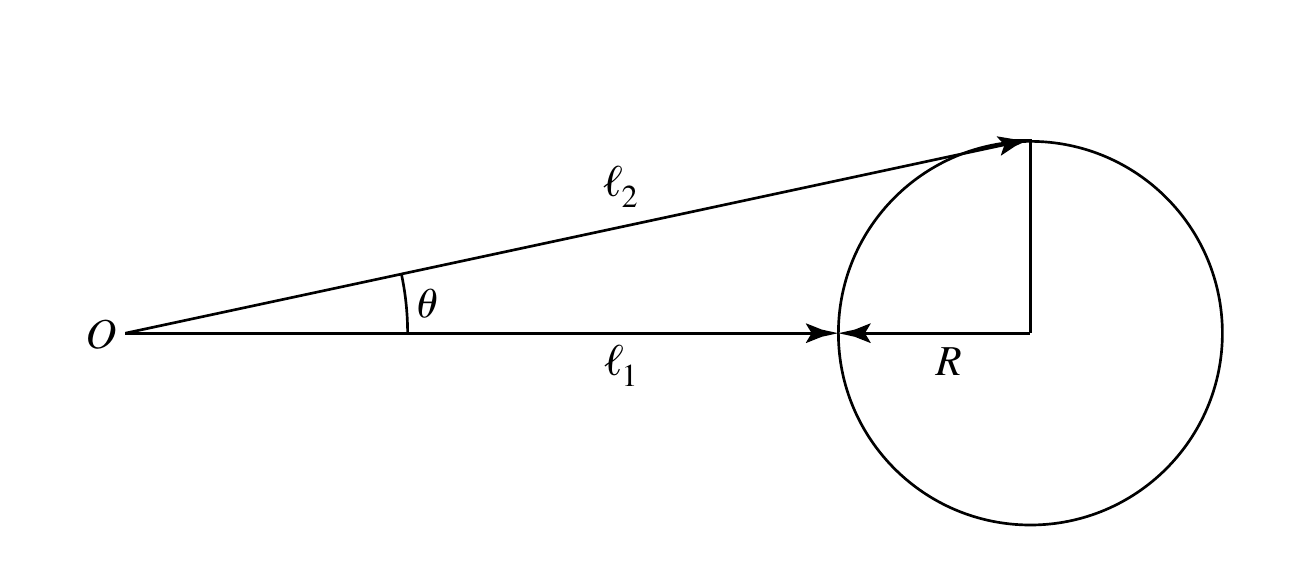
\includegraphics[scale= 0.2]{Figures/SizeView1.png}
 \caption{Διαδρομή φωτός από σφαιρικά συμμετρική πηγή. (Εικόνα από \cite{carroll_ostlie_2017})}
 \label{fig:lightpathsphere}
 \end{center}
\end{figure}
Για οπτικά πυκνή σφαίρα ακτίνας $R$ (σχήμα \ref{fig:lightpathsphere}) που υφίσταται σύντομη (στιγμιαία) αλλαγή στην λαμπρότητά της ακαριαία (στο σύστημα ηρεμίας της) και σε όλη την έκτασή της, μακρυνός παρατηρητής ($O$) καταλαβαίνει την μεταβολή αυτή από την διαφορά λαμπρότητας στο σήμα που δέχεται αρχικά από την εγγύτερη περιοχή, δηλαδή το σήμα που έχει διανύσει απόσταση $\ell_1$ , με τελευταίο σήμα το σήμα από το χείλος που διήνυσε απόσταση $\ell_2$ . Θα ισχύει
$$\ell_2 = \dfrac {\ell_1+R}{cos\theta} \simeq \ell_1+R$$
για $R<<1 $ και $cos \theta \simeq 1$, το ηλεκτρομαγνητικό σήμα από το χείλος της σφαίρας θα έχει διανύσει απόσταση μεγαλύτερη του κοντυνότερου σημείου κατά $\ell_2 - \ell_1 \simeq R$. \\
Έτσι η στιγμιαία αλλαγή στην λαμπρότητα αποτυπωνεται σε σήμα που διαρκεί $\Delta t = R/c$. Δηλαδή η διάρκεια αλλαγής στην λαμπρότητα μπορεί να χρησιμοποιηθεί για να θέσει ένα άνω όριο στις διαστάσεις της πηγής (για σφαιρικά-ισοτροπικά αντικείμενα).
Αν το σφαιρικό αυτό αντικείμενο απομακρυνόταν από τον παρατηρητή (Γη) με ταχύτητα $v$, η ακτίνα του στο σύστημα ανάφοράς μας (Γη) θα ήταν \cite{carroll_ostlie_2017}
\begin{equation}R = c\Delta t \sqrt{1-\dfrac{v^2}{c^2}}= \dfrac {c\Delta t }{\gamma} \label{eq:Radius}\end{equation}

\subsection*{Μάζα}

Για σφαιρικά συμμετρικό αντικείμενο σε ισορροπία η φωτεινότητα $L$ έχει άνω όριο το όριο \textlatin{Eddington} $ L < L_{Edd}$, όπου 
\begin{equation} L_{Edd} \approx 1.3 \cdot 10^{38} \big( \frac{M}{M_{\odot}} \big) \; erg \; s^{-1} \label{eq:Eddington}\end{equation}
Η $ L_{Edd}$ προκύπτει για υδροστατική ισορροπία όπου η πίεση είναι κυρίως πίεση ακτινοβολίας και η ύλη πλήρως ιονισμένο υδρογόνο και αποτελεί άνω όριο διότι η σφαιρική πρόσπτωση ύλης υπερισχύει της ακτινοβολίας ώστε να έχουμε σφαιρική προσαύξηση.\\
Για δεδομένη φωτεινότητα $L$, το άνω όριο μάζας από την σχέση \ref{eq:Eddington} gia $ L < L_{Edd}$ \cite{carroll_ostlie_2017}:
\begin{equation} M< \dfrac {L}{1.3\cdot 10^{38} \; erg \; s^{-1}} M_{\odot} \end{equation}
Ένα τέτοιο ποσό μάζας σε αυτές τις διαστάσεις είναι ένδειξη υπερμεγέθους μελανής οπής.
Η μάζα μελανής οπής ακτίνας $R$ από την σχέση ακτίνας \textlatin{Schwarzschild} και την σχέση \ref{eq:Radius}:
\begin{equation} M = \dfrac{Rc^2}{2G} =\dfrac {c^3\Delta t}{2G \gamma }  \end{equation}
Υπάρχουν κι άλλοι τρόποι να εκτιμήσουμε την μάζα της κεντρικής μελανής οπής, όπως η αστρική κατανομή και η δραστηριότητα σε μη-ενεργούς γαλαξίες, και έχουν να κάνουν με τον τρόπο με τον οποίο η μάζα αυτή επηρεάζει αέρια και αστέρες στο γαλαξιακό περιβάλλον\cite{AccrPower}.\\
Η άμεση παρατήρηση της κατανομής ταχυτήτων αστέρων και νεφών που αλληλεπιδρούν βαρυτικά τόσο μεταξύ τους όσο και με την κεντρική μελανή οπή σε κοντινούς γαλαξίες μπορεί να μας βοηθήσει να βγάλουμε συμπεράσματα για την κατανομή μάζας στην κεντρική περιοχή (για σφαιρική κατανομή μάζας $Μ$ με ακτίνα $r$ το θεώρημα \textlatin{virial} προβλέπει κατανομή ταχυτήτων $\overline{v}^2 \approx G M /r$ , αν υποθέσουμε ότι η δυναμική οφείλεται σε βαρυτικά φαινόμενα κυρίως και όχι π.χ. σε μαγνητικά). Παρατηρήσεις ταχυτήτων στην κεντρική περιοχή γαλαξιών είναι συνεπείς με την παρουσία υπερμεγέθους μελανής οπής σε κάθε γαλαξία.\\
Παρατηρείται συνέχεια στις ιδιότητες διαφορετικών κατηγοριών \textlatin{AGN} τόσο από υπέρλαμπρους \textlatin{AGN} σε χαμηλής λαμπρότητας (μεχρι και $10^{39}$ \textlatin{erg s}$^{-1}$) \textlatin{AGN} όσο και από ραδιογαλαξίες με ισχυρές διευρυμένες φασματικές γραμμές σε οπτικά μη-ενεργές ραδιοπηγές, αλλά ακόμα και στον Γαλαξία μας (με ραδιο-φωτεινότητα $\sim 10^{34}$ \textlatin{erg s}$^{-1}$). Τα παραπάνω είναι ενδείξεις ότι πιθανώς η ασθενής δραστηριότητα που παρατηρούμε σε μη-ενεργούς γαλαξίες είναι κατάλοιπο ενός <<νεκρού>> \textlatin{AGN}. Αυτό θα μας επέτρεπε να βγάλουμε συμπεράσματα για την μάζα της κεντρικής περιοχής ενεργών γαλαξιακών πυρήνων, αν γενικεύσουμε σχέσεις μάζας που παρατηρούμε σε κοντινούς μη-ενεργούς γαλαξίες.

\begin{figure*} 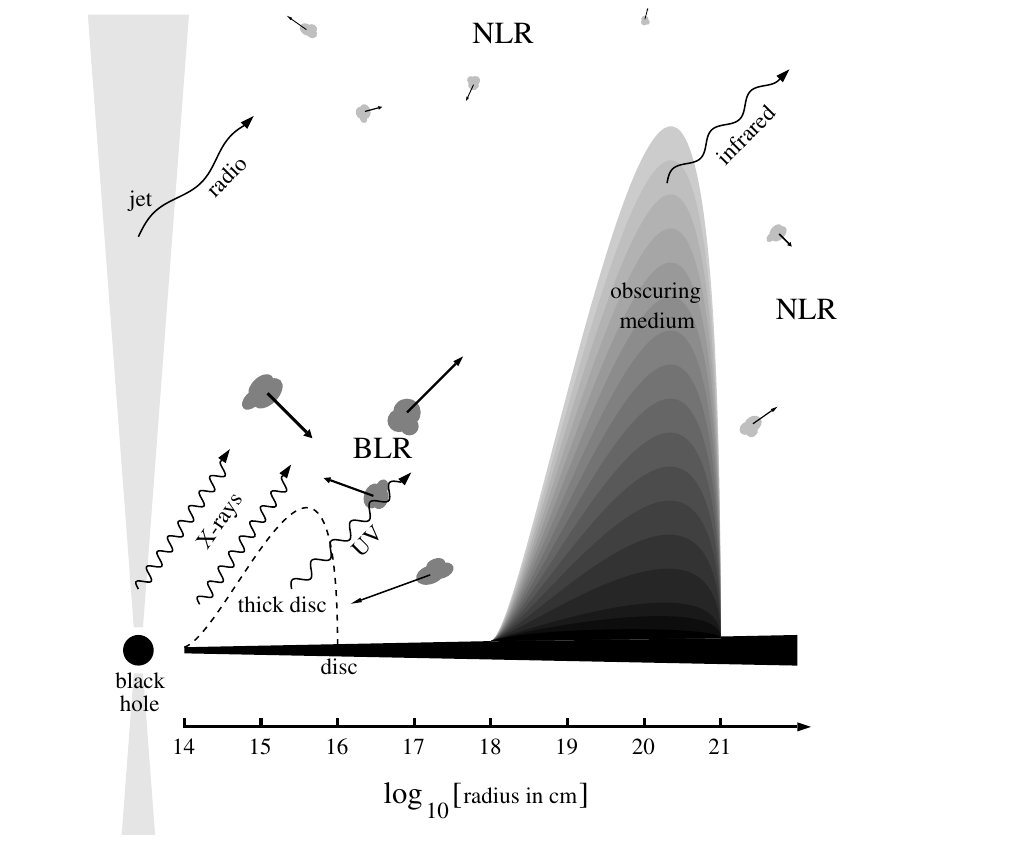
\includegraphics[width=1.2\linewidth]{Figures/AGNstucture.png} \caption{Δομή των \textlatin{AGN} που σχηματικά περιλαμβάνει στοιχεία που προτείνονται από ένα ενοποιητικό μοντέλο. Η διακεκομμένη γραμμή δείχνει πώς μπορεί να σχηματιστεί αδρός δίσκος. Το μέσο σκίασης \textlatin{(obscuring medium)} μπορεί να είναι τόρος σκόνης ή στρεβλωμένος δίσκος. \textlatin{BLR} είναι η περιοχή ευθείες παρατηρήσεις της οποίας μας δίνουν ευρείες φασματικές γραμμές εκπομπής, ενώ \textlatin{ΝLR} είναι η περιοχή ευθείες παρατηρήσεις της οποίας μας δίνουν στενές φασματικές γραμμές εκπομπής. (Εικόνα από \cite{AccrPower})}\label{fig:AGNstructure} \end{figure*}

\section{Μοντέλο μελανής οπής και δίσκου προσαύξησης}

Οι παραπάνω παρατηρήσεις- τα φάσματα εκπομπής και απορρόφησης, τα μεγέθη των παρατηρούμενων λαμπροτήτων, οι παρατηρούμενες χρονικές κλίμακες, οι θεμελιώδεις φυσικές αρχές- μας οδηγούν στο συμπέρασμα ότι η δομή των \textlatin{AGN} πρέπει να περιλαμβάνει παραγωγή ενέργειας σε μια μικρή συμπαγή περιοχή γυρω από αντικείμενο με πολύ μεγάλη μάζα.

Οι υπερμαζικές μελανές οπές είναι ευσταθείς και μπορούν να εκπέμψουν ισχυρή ακτινοβολία μέσω προσάυξησης στους \textlatin{AGN} πολύ αποδοτικά. Το πλέον καθιερωμένο μοντέλο για ενεργούς γαλαξιακούς πυρήνες είναι αυτό της υπερμαζικής μελανής οπής με δίσκο προσαύξησης (σχήμα \ref{fig:AGNstructure}). Το υλικό που ενεργοποιεί την προσαύξηση παρέχεται είτε από τοπικά αστρικά σμήνη είτε από το συνολικό αέριο και σκόνη του γαλαξία στου οποίου το κέντρο βρίσκεται\cite{AccrPower}. 
Η ύπαρξη τέτοιων μελανών οπών υποστηρίζεται και από την γενική σχετικότητα έναντι άλλων θεωριών (όπως π.χ. πυκνά σμήνη μαζικών αστέρων που σύντομα εξελίσονται σε υπερκαινοφανείς, υπερμαζικοί ασταθείς αστέρες) για τον μηχανισμό και την κεντρική περιοχή των \textlatin{AGN}\cite{AccrPower}.

\subsection{Κεντρική μελανή οπή}

Μια θεωρία βαρύτητας μας δίνει εξισώσεις κίνησης σωματίων που υφίστανται την βαρυτική επιροή σωμάτων με μεγάλη αδράνεια. Στην νευτώνεια θεώρηση, η ακτινική θέση $r(t)$ σωματίου σε τροχιά γύρω από σφαιρικά συμμετρικό μαζικό αντικείμενο μάζας $Μ$ δίνεται από την εξίσωση ενέργειας:
\begin{equation}
    \dfrac{1}{2} \Big( \dfrac{dr}{dt} \Big)^2 + V(r) = E
\end{equation}
Όπου $Ε$ σταθερή ενέργεια ανά μονάδα μάζας του σωματιδίου και 
\begin{equation}
    V(r)=h^2/2r^2- GM/r
\end{equation}
το ενεργό δυναμικό ανά μονάδα μάζας σωματίου με στροφορμή $h$.\\
Στην γενική σχετικότητα όλη η ενέργεια συνεισφέρει στην βαρυτική μάζα ενός συστήματος, συμπεριλαμβανομένου και της βαρυτικής δυναμικής ενέργειας. Ένα βαρυτικό πεδίο είναι ισχυρό όταν $GM m/r \sim mc^2$ gia σωμάτιο μάζας $m$, δηλαδή όταν η βαρυτική δυναμική ενέργειά του είναι της τάξης της ενέργειας μάζας ηρεμίας του. Για σφαιρικά συμμετρικό στάσιμο σώμα μάζας $Μ$ στο κενό η εξίσωση ενέργειας δίνεται από την λύση \textlatin{Schwarzschild}: 
\begin{equation}
    \dfrac{1}{c^2} \Big( \dfrac{dr}{d\tau} \Big)^2 + V^2(r) = E^2 \label{eq:SchwarzEnergy}
\end{equation}
Όπου $\tau$ ο ιδιόχρονος του σωματίου, η σχέση του οποίου με τον χρόνο $t$ του συστήματος συντεταγμένων είναι: 
\begin{equation}
    \dfrac{dt}{d\tau}  = E \Big(1 - \dfrac{2GM}{rc^2}  \Big)^{-1} \label{eq:SchwarzPropertime}
\end{equation}
Και το ενεργό δυναμικό στην περίπτωση αυτή είναι:
\begin{equation}
    V^2(r) =  \Big( 1 - \dfrac{2GM}{rc^2}  \Big)   \Big( 1 + \dfrac{h^2}{r^2c^2}  \Big) \label{eq:SchwarzPotential}
\end{equation}
Όπου  $h$ η σταθερή σχετικιστική στροφορμή ανά μονάδα μάζας του σωματίου που βρίσκεται σε τροχιά.\\
Καθώς η ακτινική απόσταση του σωματίου μικραίνει πλησιάζοντας την ακτίνα  \textlatin{Schwarzschild} του κεντρικού σώματος $ r \rightarrow 2GM/c^2 = R_S$ οι εξισώσεις \ref{eq:SchwarzPotential} kai \ref{eq:SchwarzPropertime} δείχνουν ότι $V \rightarrow 0$ kai $dt/d\tau \rightarrow \infty$. Για συμπαγή αντικείμενα μάζας $Μ$ η ακτίνα \textlatin{Schwarzschild} έχει φυσικό νόημα (ένα σωμάτιο μπορεί να φτάσει στην απόσταση αυτή χωρίς να ανακόπτεται από τις διαστάσεις του σώματος $Μ$) και είναι σημαντική αφού ορίζει τον ορίζοντα της μελανής οπής. Από την σχέση \ref{eq:SchwarzEnergy}, προκειμένου να ισχύει $(dr/d\tau)^2 \geq 0$, το ενεργό δυναμικό έχει ανώτατο όριο $V^2 \leq E^2$ και κατώτατο όριο το $Ω^2 \geq 0$ στην ακτίνα \textlatin{Schwarzschild}. 
Η σχέση \ref{eq:SchwarzPotential} επιτρέπει τροχιές σε αυτά τα όρια στο ενεργό δυναμικό μόνο για $ h \geq 2\sqrt{3} GM/c^2$, έτσι σωμάτια με στροφορμή $ h < 2\sqrt{3} GM/c^2$ δεν διαφέυγουν της μελανής οπής. Ευσταθείς τροχιές έχουμε για ελάχιστα της συνάρτησης $V(r)$, και συγκεκριμένα για
\begin{equation}
    r =  \frac{GM}{2c^2} \big[ H^2 - \sqrt{H^4 - 12H^2}     \big]
\end{equation}
Όπου $ H = c^2 h/GM$, με $ h \geq 2\sqrt{3} GM/c^2$. Η μικρότερη ακτίνα ευσταθούς τροχιάς γύρω από μελανή οπή \textlatin{Schwarzschild} ορίζεται $r_{min} = 6GM/c^2$ και ορίζει την επιφάνεια της μέγιστης δυνατής παραγωγής ενέργειας από τα προσπίπτοντα σωματίδια. Αφού σωμάτια που βρίσκονται από το κέντρο της μελανής οπής μέχρι την ελάχιστη αυτή ακτίνα ευσταθούς τροχιάς θα καταρεύσουν προς την μελανή οπή, σωματίδια που βρίσκονται οριακά σε απόσταση $r_{min}$ θα έχουν τον μεγαλύτερο χρόνο κατάρευσης και συνεπώς ακτινοβολίας\cite{AccrPower}.\\
Νευτώνειοι υπολογισμοί της μέγιστης αποδοτικότητας παραγωγής ενέργειας ως το πηλίκο της μέγιστης διαθέσιμης βαρυτικής δυναμικής ενέργειας προς την ενέργεια μάζας ηρεμίας δίνουν κατά προσέγγυση για μελανές οπές \textlatin{Schwarzschild}:
\begin{equation}
    \varepsilon_{max}  =  \frac{GMm/ 2 r_{min}}{mc^2} = \frac{1}{12}
\end{equation}
Για περιστρεφόμενες μελανές οπές με αξισυμμετρία στον άξονα στροφορμής μάζας $Μ$ και στροφορμής ανά μονάδα μάζας $Η$ στο κενό, η εξίσωση ενέργειας δίνεται από την λύση \textlatin{Kerr}. Για να περιγράψουμε τις μελανές οπές \textlatin{Kerr} ορίζουμε τις ποσότητες μήκους: $m = GM/c^2$ kai $\alpha = H/c$. Για τον ορίζοντα μελανών οπών \textlatin{Kerr} έχουμε διπλή λύση $r_{\pm} = m \pm \sqrt{(m^2-\alpha^2) }$ και η εξωτερική ακτίνα ορίζοντα είναι η $r_{+} = m + \sqrt{(m^2-\alpha^2) }$. Το ενεργό δυναμικό της κίνησης σε ισημερινό πεδίο μπορεί να οριστεί ως η ελάχιστη ενέργεια ανά μονάδα μάζας $E_{min}$ για την οποία η κίνηση είναι εφικτή σε ακτίνα $r_{+}$ και δίνεται από την σχέση:
\begin{equation} 
\begin{aligned}
V(r) \equiv E_{min}(r) =  {} &  \Big[\sqrt{r^2 - 2mr + \alpha^2} \sqrt{r^2h^2+ \big[r(r^2+ \alpha^2)+2 \alpha^2m \big]r}  +\\
& + 2 \alpha h m\Big] \Big[ r(r^2+ \alpha^2)+2 \alpha^2m \Big]^{-1}
\end{aligned}
\end{equation} 
Η μικρότερη ακτίνα ευσταθούς κυκλικής τροχιάς σωματίου γύρω από μελανή οπή \textlatin{Kerr} υπολογίζεται:
\begin{equation}
r_{min} = m \big[ 3 + A_2 \mp \sqrt{ (3-A_1)(3+A_1+2A_2) } \big]
\end{equation} 
Όπου $A_1 = 1+(1 - \alpha^2 /m^2)^{1/3} \big[ (1+\alpha/m)^{1/3} +(1- \alpha m)^{1/3}  \big]$, $A_2 = (3\alpha^2/m^2 + A_1^2)^{1/2}$, ενώ η σχέση έχει <<$-$>> για σωμάτια με τροχιά ομόρροπη της περιστροφής της μελανής οπής και <<$+$>> για σωμάτια με τροχιά αντίρροπη. 
Η επιφάνεια που ορίζει η μικρότερη ευσταθής ακτίνα αντιστοιχεί σε μέγιστη απόδοση παραγωγής ενέργειας\cite{AccrPower}:
\begin{equation}
\varepsilon_{max} = 1- \dfrac{r_{min} - 2m \pm (\alpha \sqrt{m}/ \sqrt{r_{min}})  } {\sqrt{ r_{min} - 3m \pm \big( 2\alpha \sqrt{m}/ \sqrt{r_{min}}\big)  }}
\end{equation}
Η απόδοση αυτή φτάνει το $40\%$ για σωμάτια με τροχιά ομόρροπη της περιστροφής της μελανής οπής και στροφορμή τέτοια ώστε $\alpha = m$. 

\subsection{Προσαύξηση}

\subsubsection*{Παροχή μάζας}

Τα περισσότερα μοντέλα ενεργών γαλαξιακών πυρήνων απαιτούν μεγάλη ποσότητα ύλης για την παραγωγή ενέργειας στην κεντρική περιοχή. Η προσάυξηση σε υπερμεγέθεις μελανές οπές είναι το κυρίαρχο και καθιερωμένο μοντέλο και απαιτεί συνεχή παροχή μάζας για την παραγωγή της παρατηρούμενης ενέργειας ακτινοβολίας. Προκειμένου να επιτευχθεί προσαύξηση, υλικό που βρίσκεται κοντά στην κεντρική μελανή οπή θα πρέπει να χάνει στροφορμή από την περιστροφή του ώστε να προσπίπτει στο κέντρο. Αυτό θα πρέπει να γίνεται με κάποιον αποδοτικό μηχανισμό και σε χρονικές κλίμακες που είναι τυπικές της γαλαξιακής εξέλιξης\cite{netzer_2013}. Το ζήτημα της παροχής μάζας (δηλαδή αερίου) έχει να κάνει τόσο με την προέλευση του αερίου όσο και με τον μηχανισμό με τον οποίο καταλήγει στην κεντρική περιοχή ώστε να χρησιμοποιηθεί ως υλικό προσαύξησης και να καταστήσει τον γαλαξιακό πυρήνα <<vενεργό>>. Έχουμε δύο περιπτώσεις προέλευσης του υλικού προσαύξησης στο καθιερωμένο μοντέλο των \textlatin{AGN}: στην πρώτη περίπτωση το υλικό προέρχεται από μια <<τοπική>> πυρηνική περιοχή (πυκνά νέφη ή αστρικά σμήνη σε ακτίνα μικρότερη των $10$ \textlatin{pc}), στην δεύτερη περίπτωση το υλικό προέρχεται από το κυρίως σώμα του γαλαξία, από διαγαλαξιακό μέσο ή από αλληλεπιδράση με άλλον γαλαξία (αέριο σε ακτίνα μεγαλύτερη του $1$ \textlatin{kpc})\cite{AccrPower}.

Όσον αφορά την περίπτωση πυρηνικού υλικού ως τροφοδότη της προσαύξησης, αν υποθέσουμε ότι το υλικό αυτό είναι αέριο και πυκνά αστρικά σμήνη, θεωρείται ότι περίπου $10^{9}$ αστέρες συγκενρώνονται σε ακτίνα $\sim 10 \; pc$ από το κέντρο του γαλαξία λόγω δυναμικών διαδικασιών που οφείλονται σε αστέρες και αέρια. Στην υπόθεση αυτή, παρακάμπτεται το πρόβλημα της μείωσης στροφορμής του υλικού, αφού αν έχει διαμορφωθεί αστρικό σμήνος στην περιοχή έχει ήδη μειωμένη στροφορμή. Όμως ακόμα κι αν έχουμε αστρικά σμήνη στην κεντρική περιοχή, ο ρυθμός με τον οποίο εκλύεται υλικό από διαδικασίες αστρικής εξέλιξης (παλιρροϊκές διαταραχές, συγκρούσεις αστέρων, αστρικός άνεμος) δεν είναι αρκετός για να παρέχει το απαιτούμενο υλικό προσαύξησης των λαμπρότερων \textlatin{AGN} που παρατηρούμε \cite{AccrPower}. \\
Αστέρες οι τροχιές των οποίων τους οδηγούν πολύ κοντά στην υπερμαζική μελανή οπή στο κέντρο του σμήνους διαλύονται από παλιρροϊκες δυνάμεις. Η εξέλιξη ενός τέτοιου σμήνους εξαρτάται από τον δυναμικό χρόνο $t_{dyn}$ (χρόνος αποκατάστασης δυναμικής ισορροπίας σε τροχιές) και τον χρόνο χαλάρωσης συστήματος δύο σωμάτων $t_{R}$ (χρόνος εκτροπής σώματος από το πεδίο βαρύτητας). Ο ρυθμός έκλυσης αερίου από παλιρροϊκές διαταραχές  
περιορίζεται από τον ρυθμό με τον οποίο οι αστρικές τροχιές μεταπίπτουν σε έναν κώνο 
ημι-ανοίγματος $\theta_{crit} \sim t_{dyn}/t_{R} $ γύρω από την διεύθυνση ακτινικής ταχύτητας λόγω απώλειας ενέργειας και στροφορμής. Ο μέγιστος ρυθμός έκλυσης αερίου για σφαιρικό αστρικό σμήνος με σχεδόν ισοτροπική κατανομή ταχυτήτων είναι της τάξης της μάζας του σμήνους προς τον χρόνο χαλάρωσης ή της τάξης μίας αστρικής μάζας προς δυναμικό χρόνο: αυτός ο ρυθμός δεν είναι αρκετός για να εξηγήσει τις μεγαλύτερες παρατηρούμενες λαμπρότητες μέσω ακτινοβολίας προσαύξησης, εκτός αν υπάρχει κάποιος μηχανισμός που ωθεί τους αστέρες σε μεγάλο αριθμό συγκρούσεων μεταξύ τους ώστε να υπάρξει απελευθέρωση μεγαλύτερης μάζας. Επίσης, όταν η κεντρική υπερμεγέθης μελανή οπή ξεπεράσει τις $\sim 10^8$ M$_\odot$, οι παλιρροϊκές δυνάμεις δεν είναι πλέον ικανές να διαλύσουν έναν αστέρα πριν αυτός καταρεύσει στην μελανή οπή- όταν ο αστέρας καταρρέει χωρίς να διαλυθεί, αυτό γίνεται με σχετικά μικρή απώλεια ενέργειας σε ηλεκτρομαγνητική ακτινοβολία\cite{AccrPower}. \\
Πυκνά αστρικά σμήνη όπως αυτά που περιγράψαμε δεν μπορούν να σχηματιστούν ως αποτέλεσμα δυναμικής χαλάρωσης βαρυτικά αλληλεπιδρώντων σωμάτων (στο πρότυπο των δύο σωμάτων), αφού θα κατέληγαν σε μικρό πυρήνα αστέρων με πολύ μεγάλες ταχύτητες που θα διαλύονταν από συγκρούσεις\cite{AccrPower}. Έτσι, αν επικεντρωθούμε σε δυναμική αερίων, πρέπει να υπάρχει μηχανισμός που συγκεντρώνει το διαθέσιμο αέριο από μια αρχικά μεγάλη περιοχή σε μικρό όγκο και να εξηγεί την απώλεια στροφορμής ώστε να προσπίπτει προς προσαύξηση. %Οι τοπικοί μηχανισμοί, όπως είδαμε ακόμα κι αν πυκνά αστρικά σμήνη διατίθενταν στην πυρηνική περιοχή του γαλαξία, δεν επαρκούν. 

Παρατηρήσεις υποδεικνύουν ότι εκτός του γαλαξιακού πυρήνα υπάρχουν μεγάλα ποσά αερίου υπό μορφή διαστρικού μέσου, οπότε εξετάζουμε τον μηχανισμό που μπορεί να μεταφέρει τα αέρια αυτά μέσω τυρβώδους ιξώδους ροής όπως στο μοντέλο $\alpha-$δίσκων που θεωρείται ότι λειτουργεί για την μεταφορά μάζας και προσαύξηση σε διπλά αστρικά συστήματα αστέρα-μελανής οπής. Στο μοντέλο αυτό ($\alpha-$δίσκων) θεωρούμε ότι το αέριο έχει ιξώδες $\eta = \alpha c_s H$, όπου $c_s$ η ταχύτητα του ήχου, $H$ η κλίμακα ύψους του δίσκου και $\alpha$ παράμετρος προσαύξησης ($\alpha=0$ όταν δεν έχουμε προσαύξηση). Για συμβατικές παραδοχές της φυσικής κατάστασης του αερίου και με παράμετρο προσάυξησης $\alpha \leq 1$ μια απλή εκτίμηση δίνει χρόνο ροής προς την πυρηνική περιοχή $10^9$ \textlatin{yr} για αέριο που βρίσκεται σε ακτίνα μεγαλύτερη των $10$ \textlatin{pc} \cite{AccrPower}. Έτσι, ένας συμβατικός δίσκος προσαύξησης στο μοντέλο αυτό δεν μπορεί να παρέχει σταθερά υλικό προσαύξησης στην πυρηνική περιοχη. Έπειτα, οι λεπτοί δίσκοι προσαύξησης (που αποδίδουν μεγαλύτερη λαμπρότητα στο μοντέλο αυτό) είναι βαρυτικά ασταθείς σε μεγάλες ακτίνες όπου είναι πιο εύκολο να ψυχθούν κατά περιοχές και οι ψυχρές περιοχές να αποσυζευχθούν οδηγώντας σε επιβράδυνση της προσαύξησης.\\
Στο πρότυπο των $\alpha-$δίσκων, λοιπόν, δεν μπορεί να διατηρηθεί θερμή ροή προσαύξησης με τα συμβατικά χαρακτηριστικά που αναφέραμε, οπότε χρειαζόμαστε έναν μηχανισμό με ενεργό παράμετρο προσαύξησης $\alpha \gg 1$. Έχουν προταθεί μηχανισμοί που θα μπορούσαν να αποδόσουν $\alpha \gg 1$ με σύζευξη ρευστού σε πολύ διαφορετικές ακτινικές κλίμακες. Δύο τέτοιοι μηχανισμοί είναι μαγνητικά πεδία γαλαξιακής κλίμακας και μη αξισυμμετρικές βαρυτικές αστάθειες. Αν ένα μεγάλης κλίμακας πολοειδές μαγνητικό πεδίο υπήρχε σε γαλαξίες που <<φιλοξενούν>> υπερμεγέθη μελανή οπή, οι μαγνητοϋδροδυναμικές ροπές που γενά η στρέψη του πεδίου θα μπορούσαν να συζεύξουν αέριο σε διαφορετικές ακτινικές κλίμακες και να μεταφέρουν υλικό προς το κέντρο μειώνοντας την στροφορμή του\cite{AccrPower}. Σε αυτήν την διαδικασία δημιουργούνται τοροειδή πεδία που αυξάνουν την μαγνητική πίεση και παραλληλίζουν την εκροή ύλης με τον άξονα περιστροφής εξηγώντας παρατηρούμενους πίδακες. %Ενδείξεις τέτοιων μανητικών πεδίων υπαρχουν για τον Γαλαξία μας και σε κάποιους κοντινούς γαλαξίες, χωρίς όμως να είναι ξεκάθαρο αν η έντασή τους είναι αρκετή.   
Ένας άλλος προτεινόμενος μηχανισμός είναι μη αξισυμμετρικές δομές (όπως ράβδοι από αστέρες και αέριο, ελλειψοειδείς δίσκοι και δακτύλιοι, γαλαξίες-συνοδοί) και διαταραχές που προκαλούνται από παλιρροϊκές αλληλεπιδράσεις με άλλους γαλαξίες ή συγχωνεύσεις με άλλους γαλαξίες. Η αρχή λειτουργίας του μηχανισμού αυτού είναι ότι καθώς αέριο περιστρέφεται γρηγορότερα από την ράβδο του γαλαξία, πλησιάζοντάς την επιταχύνεται προς το ελάχιστο του βυθίσματος δυναμικού κι έπειτα επιβραδύνεται και συμπιέζεται καθώς προπερνά την ράβδο. Το ωστικό κύμα του αερίου στην μπροστινή όψη της ράβδου (που οδηγεί την κίνηση) χάνει στροφορμή την οποία παρέχει στην ράβδο με αποτέλεσμα να ρέει προς το κέντρο. Παρόμοια ροή αερίου θα έχουμε για διαταραχές που προκαλούνται από αλληλεπίδραση  με άλλους γαλαξίες όπου προκύπτουν δομές σαν ράβδοι. Ακόμα, όμως, και σε αύτην την περίπτωση το αέριο δεν ρέει μέχρι το κέντρο, αφού όσο μια μάζα αερίου προχωρά προς το κέντρο τόσο ασθενεί η επίδραση της ράβδου. Το αέριο τυπικά φθάνει μέχρι ακτίνα $\sim 1$ \textlatin{pc} όπου ούτε η ιξώδης ροή δεν αρκεί για να το μεταφέρει με ικανοποιητικό ρυθμό προς το κέντρο, όμως αν η ίδια η μάζα του αερίου που συσσωρεύεται γίνει δυναμικά σημαντική μπορεί να έχουμε μη-αξισυμμετρικές δυναμικές αστάθειες και ανακατανομή στροφορμής που ωθεί το αέριο προς την κεντρική περιοχή\cite{AccrPower}.    

\subsubsection*{Δίσκος προσαύξησης}

Σε γαλαξιακές χωρικές και χρονικές κλίμακες, η παροχή υλικού προσαύξησης στις υπερμεγέθεις μελανές οπές εξαρτάται από μηχανισμούς όπως συγκρούσεις και συγχωνεύσεις γαλαξιών, δυναμικές αστάθεις όπως ράβδοι, μαγνητικά πεδία που φέρνουν υλικό σε αποστάσεις $1-10$ \textlatin{pc} από την κεντρική μελανή οπή. Σε κοντινότερες ακτινικές αποστάσεις ο μηχανισμός προσαύξησης βασίζεται στην βαρυτική έλξη της μελανής οπής, την ιδιοβαρύτητα του υλικού, την τοπική υδροδυναμική πίεση και πίεση ακτινοβολίας, αστρικούς ανέμους, υπερκαινοφανείς εκρήξεις, μαγνητικό και θερμικό ιξώδες του αερίου. Αέριο με χαμηλή στροφορμή προsπίπτει σφαιρικά στην μελανή οπή, ενώ αέριο με υψηλή στροφορμή προσπίπτει στην μελανή οπή μέσω κεντρικού δίσκου προσαύξησης που παρέχει έναν μηχανισμό ιξώδους ροής που μειώνει την στροφορμή\cite{netzer_2013}.
Η προσαύξηση ύλης με σημαντική στροφορμή σε μελανή οπή συνοδεύεται από σχηματισμό δίσκου από το υλικό πρασάυξησης. Τέτοιοι δίσκοι πρέπει να σχηματίζονται και σε μελανές οπές αστρικής προέλευσης και σε υπερμεγέθεις μελανές οπές.

Μοντέλα δίσκων προσαύξησης βασίζονται σε παρατηρήσεις μελανών οπών σε διπλά συστήματα και ο μηχανισμός προσαύξησης γενικεύεται για υπερμεγέθεις μελανές οπές. Για προσαύξηση σε μελανή οπή τα σύγχρονα μοντέλα προβλέπουν την ροή αερίου είτε σε λεπτούς δίσκους που περιστρέφονται γύρω από την μελανή οπή είτε ένα αδρό χαοτικό νέφος. Για φωτεινότητα ακτίνων Χ που υπερβαίνει το όριο \textlatin{Eddington} είναι πιο πιθανή η εικόνα του αδρού νέφους, ενώ για υπο-\textlatin{Eddington} φωτεινότητα η εικόνα του λεπτού δίσκου. Για φωτεινότητα χαμηλότερη της φωτεινότητας \textlatin{Eddington} ώστε $L \lesssim 10^{-2} L_{Edd}$ θερμικές αστάθειες λόγω χαμηλής οπτικής πυκνότητας μπορούν να διαταράξουν την εσωτερική περιοχή λεπτού δίσκου και να μεταπίψει σε αδρό νέφος, αλλά ακόμα και για φωτεινότητα $L\lesssim 10^{-4} L_{Edd}$ έχουμε ασταθείς λεπτούς δίσκους\cite{Lightman1974}. 

Σε ένα διαφορικά περιστρεφόμενο μέσο (όπως είναι το υλικό στον δίσκο πρσαύξησης) οι εφαπτομενικές τάσεις ανάμεσα στα διάφορα στρώματα (οι οποίες σχετίζονται με την ύπαρξη μαγνητικού πεδίου), η τυρβώδης ροή και το μοριακό και ηλεκτρομαγνητικό ιξώδες είναι οι μηχανισμοί που μεταφέρουν στροφορμή\cite{ShakuraBlackHoles} έτσι ώστε το υλικό να καταρεύσει σπειροειδώς προς το κέντρο. Η ενέργεια που χάνει το υλικό (αέριο) μπορεί να μετατραπεί σε ηλεκτρομαγνητική ακτινοβολία με πολύ μεγάλη απόδοση (είδαμε από 4\% έως 40\% για αντικείμενα \textlatin{Kerr}) ή μπορεί να μετατραπεί σε κινητική ενέργεια του αερίου με αποτέλεσμα να διαφύγει του δίσκου ή μπορεί να θερμάνει το αέριο με την θερμική ενέργεια να μεταφέρεται στην μελανή οπή (\textlatin{advection accretion flow})\cite{netzer_2013}.

Το πιο χρήσιμο μοντέλο δίσκων προσαύξησης είναι αυτό των $\alpha-$δίσκων, ένα νευτώνειο μοντέλο (περιγράφει καλά υλικό σε ακτίνα $R>3R_{Schw}$) που βασίζεται σε παρατηρήσεις μελανών οπών σε διπλά συστήματα και περιγράφει λεπτούς δίσκους. Στο μοντέλο αυτό παραδεχόμαστε τυρβώδη ροή, μη-γραμμικές διαταραχές (δηλαδή αλληλεπίδραση μεταξύ τυρβώδων παλμών) και ως αποτέλεσμα μια αυτο-συντηρούμενη τύρβη\cite{ShakuraBlackHoles}. 
Για μη-μηδενικά μαγνητικά πεδία στους δίσκους, αστάθειες διατμητικής τάσης συντηρούν επίσης τυρβώδη ροή η οποία είναι ο κυρίαρχος παράγοντας που μεταφέρει στροφορμή\cite{Blackman98}. \\
Η δομή και η ακτινοβολία στατικών δίσκων καθορίζονται από τρείς φυσικές παραμέτρους: την μάζα της μελανής οπής $Μ$, τον ρυθμό προσαύξησης $\dot M$ (ή την συνολική φωτεινότητα του δίσκου $L = \zeta \dot M c^2$, όπου $\zeta$ ο συντελεστής απόδοσης της παραγωγής ενέργειας) και την παράμετρο $\alpha$, η οποία χαρακτηρίζεται από το επίπεδο τυρβώδους ροής και από χαοτικά μικρής κλίμακας μαγνητικά πεδία\cite{ShakuraInstability}.
\begin{equation}
    \alpha = \dfrac{v_t l_t}{v_s Η} + \dfrac{B}{4\pi \rho v_s^2}
\end{equation}
Όπου $v_t$ kai $v_s$ η ταχύτητα τυρβώδους ροής και η θερμική ταχύτητα αντίστοιχα, $B^2/8\pi$ η ενεργειακή πυκνότητα του χαοτικού μαγνητικού πεδίου, $\rho v_s^2/2$ η θερμική ενεργειακή πυκνότητα του υλικού στον δίσκο, $l_t$ το μήκος τυρβώδους ανάμειξης και $Η$ το ημι-ύψος του δίσκου.\\
Η φωτεινότητα, όπως έχουμε δεί, φαινομενικά φράσσεται από την φωτεινότητα \textlatin{Eddington} $$L_{Edd} = 1.3\times10^{38} \Big(\dfrac{M}{M_\odot}   \Big) \; erg \; s^{-1}$$ 
η οποία προκύπτει εξισώνοντας την βαρυτική δύναμη με την δύναμη πίεσης ακτινοβολίας για πλάσμα στο εσωτερικό του δίσκου. Για φωτεινότητες κοντά στο όριο \textlatin{Eddington} $L/L_{Edd} \gtrsim \frac{1}{50} (M_\odot/\alpha M)^{1/8}$ ο δίσκος αποτελείται από τρείς περιοχές, την <<vεσωτερική>> ζώνη (ζώνη Α) όπου η πίεση ακτινοβολίας είναι μεγαλύτερη από την πίεση αερίου και η σκέδαση ελεύθερων ηλεκτρονίων κυριαρχεί σε σχέση με άλλες διαδικασίες απορρόφησης ακτινοβολίας. Αυτή η περιοχή εκπέμπει το μεγαλύτερο ποσό ενέργειας ακτινοβολίας του δίσκου και οι διαδικασίες \textlatin{Compton} καθορίζουν το παρατηρούμενο φάσμα. Σε μεγαλύτερη ακτίνα από την μελανή οπή βρίσκεται η ζώνη Β όπου η πίεση πλάσματος είναι μεγαλύτερη από την πίεση ακτινοβολίας, αλλά η σκέδαση ελεύθερων ηλεκτρονίων υπερισχύει στην διάδοση ακτινοβολίας. Πέρα από την ζώνη Β υπάρχει η ψυχρότερη περιοχή Γ όπου φαινόμενα απορρόφησης συμβάλουν στην οπτική πυκνότητα\cite{ShakuraInstability}.
Για $L/L_{Edd} < \frac{1}{50} (M_\odot/\alpha M)^{1/8}$  δεν έχουμε την ασταθή περιοχή Α. 

\subsection{Άλλα χαρακτηριστικά των \textlatin{AGN}}

Άλλα δομικά χαρακτηριστικά των \textlatin{AGN} πιθανώς υπάρχουν γύρω από την μελανή οπή και επηρεάζουν το φάσμα λόγω της θέσης τους, της πυκνότητας ύλης σε αυτά, του ιονισμού σε αυτά, της σύνθεσης ή ταχύτητάς τους (σχήμα \ref{fig:AGNstructure}). Θα εξετάσουμε μόνο μερικά από αυτά. 

\subsubsection*{Περιοχή διευρυμένων φασματικών γραμμών \textlatin{(Broad Line Region)}}
Πρόκειται για περιοχή με νέφη υψηλής χωρικής πυκνότητας σωματιδίων (\textlatin{n}$_{e} \sim 10^{10}$ \textlatin{cm}$^{-3}$) με μεγάλη επιφανειακή πυκνότητα (πυκνότητα στήλης) Ν$_{Η} \sim 10^{23}$ \textlatin{cm}$^{-2}$ γύρω από την υπερμεγέθη μελανή οπή και τον δίσκο προσαύξησης. Για πολύ λαμπρούς \textlatin{AGN} η περιοχή αυτή βρίσκεται σε ακτίνα $0.1-1$ \textlatin{pc} από την κεντρική μελανή οπή. Τα νέφη αυτά διατηρούνται για πολούς δυναμικούς χρόνους είτε επειδή είναι περιορισμένα είτε επειδή είναι μέλη μεγαλύτερων σωμάτων με ιδιοβαρύτητα (όπως π.χ. αστέρες). Η τυπική κεπλεριανή ταχύτητα τέτοιων νεφών είναι $ \sim 3000$ \textlatin{km s}$^{-1}$ kai αυτό αποτυπώνεται στα πλάτη των φασματικών γραμμών εκπομπής\cite{netzer_2013}.

\subsubsection*{Περιοχή στενών φασματικών γραμμών \textlatin{(Narrow Line Region)}}

Όπως φαίνεται και στο σχήμα \ref{fig:AGNstructure}, η περιοχή στενών φασματικών γραμμών είναι περιοχή με νέφη χαμηλότερης πυκνότητας (\textlatin{n}$_{e} \sim 10^{4}$ \textlatin{cm}$^{-3}$) με επιφανειακή πυκνότητα Ν$_{Η} \sim 10^{20-21}$ \textlatin{cm}$^{-2}$ γύρω από την υπερμεγέθη μελανή οπή. Η περιοχή αυτή βρίσκεται σε ακτίνα $> 3$ \textlatin{pc} από την κεντρική μελανή οπή για πολύ λαμπρούς \textlatin{AGN} και είναι πιο μαζική από την \textlatin{Broad Line Region}. Η τυπική ταχύτητα (αν θεωρήσουμε ότι τα νέφη αυτά βρίσκονται στο βαρυτικό πεδίο του γαλαξία) είναι της τάξης των $300$ \textlatin{km s}$^{-1}$. Το αέριο αυτό μπορεί να σχηματίσει διάφορες δομές, χρησιμοποιούμε τον όρο <<νέφος αερίων>> ως γενική περιγραφή\cite{netzer_2013}. 

\subsubsection*{Αέριο υψηλού ιονισμού}

Θεωρούμε ότι σε χωρική κλίμακα $0.1-10 $ \textlatin{pc} από το κέντρο υπάρχει περιοχή με επιφανειακή πυκνότητα Ν$_{Η} \sim 10^{21-23}$ \textlatin{cm}$^{-2}$ και πυκνότητα ικανή να παράξει ιονισμό 10-100 φορές υψηλότερο απ> ότι το αέριο sthn \textlatin{BLR} kai thn \textlatin{NLR.} Για το αέριο αυτό αναμένουμε ισχυρή απορρόφηση και εκπομπή στις ακτίνες Χ\cite{netzer_2013}.

\subsubsection*{Τόρος}
%Θα πρεπει ισως μα εξιγισεις οτι η υποθεση του τορου προερχεται απο την υπαρξη Ι/ΙΙ τυπου αντικειμενων, και η απλοικη υποθεση οτι υπαρχει υλικο σε μορφη τορου και η διαδοροποιηση αναμεσα σε Ι/ΙΙ ειναι καθαρα γεωμετρικο φαινομενο. 
Προκειμένου να εξηγηθεί η διαφοροποίηση μεταξύ \textlatin{AGN} τύπου Ι και τύπου ΙΙ ως γεωμετρικό φαινόμενο, θεωρούμε ότι υπάρχει τοροειδής δομή από αέριο, μοριακό αέριο και σκόνη σε περιοχή μεταξύ $0.1$ και $10$ \textlatin{pc} από την κεντρική μελανή οπή με πυκνότητα αερίου $\sim 10^{4}-10^{7}$ \textlatin{cm}$^{-3}$, επιφανειακη πυκνότητα που κυμαίνεται N$_{H} \sim 10^{22-24}$ \textlatin{cm}$^{-2}$ και κεπλεριανές ταχύτητες της τάξης των $1000$ \textlatin{km  s}$^{-1}$. Ο τόρος αυτός είναι οπτικά αδιαφανής για όλα τα μήκη κύματος εκτός του υπερύθρου και πιθανότατα σκιάζει την εκπομπή από τον δίκο προσάυξησης και την \textlatin{BLR} για παρατήρηση από ορισμένες διευθύνσεις\cite{netzer_2013}.

\subsection{Θεμελιώδη φυσικά μεγέθη συστήματος προσάυξησης}

\subsubsection*{Χαρακτηριστικές χρονικές κλίμακες}

Οι χαρακτηριστικοί χρόνοι μας δίνουν πληροφορίες για την συμπεριφορά ενός συστήματος. Για στατικούς, λεπτούς (δηλαδή ψυχρούς κεπλεριανούς) $\alpha-$δίσκους η μικρότερη χρονική κλίμακα είναι ο δυναμικός χρόνος (ο χρόνος ώστε να επέλθει δυναμική ισορροπίa)\cite{spruit2010accretion}
\begin{equation}
    t_{dyn} = \Big( \dfrac{GM}{r^3} \Big)^{-1/2}
\end{equation}
όπου $M$ η μάζα κεντρικής μελανής οπής και $r$ η απόσταση από αυτήν.\\
Η χρονική κλίμακα για την ακτινική μετακίνηση μέσα στον δίσκο για απόσταση $r$ είναι ο χρόνος ιξώδους
\begin{equation}
    t_{visc} = \dfrac{2f}{3 \alpha \Omega}   \Big( \dfrac{r}{H} \Big)^{2}
\end{equation}
όπου $f=1-\big(\frac{r_i}{r})^{1/2}$ με $r_i$ την εσωτερική ακτίνα του δίσκου, $H$ το ημι-ύψος του δίσκου και $\Omega$ η κεπλεριανή περιστροφή του δίσκου.\\
Οι θερμικές χρονικές κλίμακες είναι ο χρόνος ψύξης και ο χρόνος θέρμανσης. Αν $E_t$ η θερμική ενέργεια (ενθαλπία) του δίσκου ανά μονάδα επιφάνειας και $W_\eta=(9/4) \Omega^2 \eta \Sigma$ είναι ο ρυθμός θέρμασης λόγω ιξώδους διάχυσης (όπου $\eta$ το ιξώδες και $\Sigma$ η επιφανειακή πυκνότητα του δίσκου), τότε η χαρακτηριστική χρονική κλίμακα θέρμανσης
\begin{equation}
    t_{h} = \dfrac{E_t}{W_\eta}
\end{equation}
Ομοίως, ο χαρακτηριστικός χρόνος ψύξης
\begin{equation}
    t_{c} = \dfrac{E_t}{2 \sigma_r T_s^4}
\end{equation}
όπου η επιφανειακή θερμοκρασία εκφράζεται ως συνάρτηση μάζας κεντρικής μελανής οπής $M$ kai ρυθμού προσαύξησης $\dot M$ $$ \sigma_r T_s^4 = \dfrac{GM}{r^3} \dfrac{3\dot M}{8\pi} \Big[ 1-\big(\frac{r_i}{r})^{1/2}\Big]$$
Για λεπτούς δίσκους οι δύο αυτές κλίμακες συμπίπτουν, αφού η διάχυση ιξώδους ενέργειας ισορροπείται τοπικά από την ακτινοβολία του δίσκου από την διπλή επιφάνειά του. Σε αδρούς δίσκους \textlatin{ADAF (advection dominated accretion flow)} δεν υπάρχει αυτή η ισορροπία, αφού η μεταφορά \textlatin{(advection)} θερμότητας με την ροή προσαύξησης δεν είναι αμελητέα- τότε $t_c>t_h$ \cite{spruit2010accretion}.\\
Οι ακτίνες Χ παράγονται από διαδικασίες αντιστρόφου σκεδασμού \textlatin{Compton.} Η χρονική κλίμακα ψύξης (ελάτωσης ενέργειας) των θερμικών ηλεκτρονίων μέσω της αντίστροφης σκέδασης \textlatin{Compton} sτο μη-σχετικιστικό όριο ($\gamma \approx 1$) είναι
\begin{equation}
    t_{Compt} = \dfrac{6\pi G^2 m_e}{\sigma_T c^4} \dfrac{\xi ^2}{\zeta} \dfrac{M_{BH}^2}{\dot M} 
\end{equation}
Όπου $\xi$ η ακτινική απόσταση σε μονάδες ακτίνας \textlatin{Schwarzschild} $R=\xi R_{Schw}$ και $\zeta$ η απόδοση της διαδικασίας προσαύξησης, οπότε η λαμπρότητα των φωτονίων πρίν την σκέδαση (\textlatin{seed photons}) $L_{seed}=\zeta \dot{M} c^2$.
 
Παρατηρούμε ότι η χαρακτηριστική χρονική κλίμακα δυναμικού χρόνου εξαρτάται από την μάζα μελανής οπής $M$, ενώ οι χαρακτηριστικές χρονικές κλίμακες ιξώδους πρόσπτωσης και θερμικών διαδικασιών εξαρτώνται από την μάζα μελανής οπής και από την προσαύξηση, είτε με ευθεία εξάρτηση από τον ρυθμό προσάυξησης $\dot M$, είτε από τον όρο που μοντελοποιεί την τυρβώδη προσαύξηση  $\alpha$. Έτσι συμπεραίνουμε πως τα μεγέθη της μάζας μελανής οπής και του ρυθμού προσάυξησης είναι θεμελιώδεη για την συμπεριφορά του συστήματος προσαύξησης. 

\subsubsection*{Διαταραχές πρώτης τάξης στον δίσκο}

Η εφαρμογή της θεωρίας διαταραχών (έστω και πρώτης τάξης) για σύστημα προσαύξησης δεν είναι τετριμμένη διαδικασία. Η φυσική περιγραφή για σύστημα προσάυξησης στο απλό μοντέλο των $\alpha$-δίσκων απαιτεί\cite{ShakuraInstability} εξίσωση κεπλεριανής κίνησης, εξίσωση συνέχειας, εξίσωση διατήρησης ορμής, υδροστατική εξίσωση, εξίσωση τάσεων ιξώδους, εξίσωση παραγωγής ενέργειας λόγω τριβής, εξίσωση απώλειας ενέργειας λόγω ακτινοβολίας και καταστατική εξίσωση.

Αποτελέσματα εργασιών πάνω στην θεωρία μικρών γραμμικών διαταραχών στο πρότυπο της τυρβώδους προσαύξησης δίνουν τους εξής συσχετισμούς\cite{Blackman98} \\
Για λεπτούς $\alpha$-δίσκους:\\
\begin{equation}
    \frac{\Delta L_\nu}{L_\nu} \propto \alpha M_{BH}^{1/2} R^{3/4} \frac{H}{R}
\end{equation}

Για αδρούς \textlatin{ADAF} δίσκους:\\
\begin{equation}
    \frac{\Delta L_\nu}{L_\nu} \propto \alpha^2 M_{BH}^{1/2} R^{3/4} \frac{H}{R}
\end{equation}
Όπου $L_\nu$ η λαμπρότητα του δίσκου και $\Delta L_\nu$ διαταραχή σε αυτήν, $\alpha$ η παράμετρος τυρβώδους προσαύξησης, $R$ η ακτίνα του δίσκου, $M_{BH}$ η μάζα κεντρικής μελανής οπής και $H$ το ημι-ύψος του δίσκου.

Βλέπουμε, λοιπόν, πως και στην πρώτη προσέγγυση της θεωρίας διαταραχών η μάζα μελανής οπής και η παράμετρος προσαύξησης παίζουν σημαντικό ρόλο.





 % Review of the Literature
	
	\chapter{Διαδικασίες ακτινοβολίας και παρατηρήσεις στις ακτίνες Χ} 

Θα παρουσιάσουμε τις μη-θερμικές φυσικές διαδικασίες ακτινοβολίας οι οποίες σχετίζονται με το φάσμα ακτινοβολίας των ενεργών γαλαξιακών πυρήνων.

\section{Σχετικιστική κινηματική και ισχύς ακτινοβολίας}

Η συνολική ισχύς ακτινοβολίας που εκπέμπεται από φορτισμένο σωμάτιο (για εκπομπή συμμετρική σε όλες τις διευθύνσεις) είναι $$P = \dfrac{dW}{dt} = \dfrac{dW^\prime}{dt^\prime}=P^\prime$$
αναλλοίωτη σε μετασχηματισμούς \textlatin{Lorentz}, καθώς το χρονικό διάστημα $dt=\gamma dt^\prime$ και η ακτινοβολούμενη ενέργεια στο διάστημα αυτό $dW= \gamma dW^\prime$, για $Κ$ σύστημα αναφοράς παρατηρητή και $Κ^\prime$ σύστημα αναφοράς στιγμιαίας ηρεμίας, δηλαδή στο οποίο το σωμάτιο για απειροστά μικρό χρονικό διάστημα να θεωρείται ακίνητο (αφού το σωμάτιο επιταχύνεται) \cite{1986rpa..book.....R}.
Οπότε βάσει της φόρμουλας \textlatin{Larmor}  $ P= \frac{2q^2 \dot{v}^2}{3c^3} $ για ακτινοβολία από επιταχυνόμενο φορτίο, έχουμε: $$ P=P^\prime =  \frac{2q^2 }{3c^3} |\mathbf{a^\prime}|^2$$
Ισχύει ότι η τετρα-ταχύτητα και η τετρα-επιτάχυνση είναι ορθογώνιες $a_\mu U^\mu = 0 $, και στο σύστημα στιγμιαίας ηρεμίας ου φορτισμένου σωματιδίου $Κ^\prime$ έχουμε $ \mathbb{U^\prime}= (c,  \vec{0})$, οπότε  $a_0 = 0$ . \\
Άρα $ |\mathbf{a^\prime}|^2 = a^\prime_0a^\prime^0 + a^\prime_ja^\prime^j=  \vec{a^\prime}\cdot \vec{a^\prime}   $, οπότε η ισχύς\cite{1986rpa..book.....R}:
$$ P=P^\prime =  \frac{2q^2 }{3c^3}  \vec{a^\prime}\cdot \vec{a^\prime} $$
Για το σύστημα στιγμιαίας ηρεμίας $K^\prime$ του σωματιδίου 
\begin{subequations}
\label{eq:PowerComp}
\begin{align}
a^\prime_{\parallel }  = \gamma^3 a_{\parallel }   \label{eq:PowerCompA} \\ 
a^\prime_{\bot }  = \gamma^2 a_{\bot }   \label{eq:PowerCompB} 
\end{align}
\end{subequations}
όπου $ a_{\parallel }$ και $a_{\bot }$ η παράλληλη και κάθετη συνιστώσα της $\vec{a^\prime}$ στην διεύθυνση της κίνησης $\vec{v}$. Οπότε η ισχύς\cite{1986rpa..book.....R}:
$$  P=P^\prime =  \frac{2q^2 }{3c^3}  \vec{a^\prime}\cdot \vec{a^\prime} = \frac{2q^2 }{3c^3} ( a^\prime^2_{\parallel } + a^\prime^2_{\bot })  = \frac{2q^2 }{3c^3} \gamma^4 (\gamma^2 a^2_{\parallel } + a^2_{\bot }) $$
Για συστήματα αναφοράς $Κ$ και $Κ^\prime$ που κινείται με ταχύτητα $v$ ως προς το πρώτο, οι
σχέσεις παρέκλισης φωτός είναι\cite{1986rpa..book.....R}:
\begin{subequations}
\label{eq:aberration}
\begin{align}
tan \theta = \dfrac{sin\theta^\prime}{\gamma (cos \theta^\prime +v/c)}    \label{eq:aberrationA} \\ 
cos \theta = \dfrac{cos \theta^\prime +v/c}{1+(v/c)cos\theta^\prime}   \label{eq:aberrationB} 
\end{align}
\end{subequations}

Η αζιμουθιακή γωνία $\phi$ μένει αναλλοίωτη, η πηγή του φωτεινού σήματος $Κ^\prime$ κινείται με ταχύτητα $v$ και εκπέμπει φωτεινό σήμα που σχηματίζει γωνία $\theta^\prime $ με το διάνυσμα $v$ στο $Κ^\prime$.
Αν έχουμε εκπομπή ενέργειας $dW^\prime$ σε στερεά γωνία $d\Omega^\prime=sin\theta ^\prime d\theta^\prime d\phi^\prime$ υπό γωνία $\theta ^\prime $ με τον $x$-άξονα (ισοτροπία), τότε\cite{1986rpa..book.....R}:
\begin{center}
$ d\Omega = d\mu d\phi $ και   
$ d\Omega^\prime= d\mu ^\prime d\phi $
\end{center}
όπου $\mu = cos\theta$ kai $\mu^\prime = cos\theta^\prime$ (και η αζιμουθιακή γωνία $\phi$ μένει αναλλοίωτη). Ο μετασχηματισμός \textlatin{Lorentz} για την $0$-συνιστώσα της τετρα-ορμής $dW = \gamma(1+\beta \mu^\prime)dW'$ και από την σχέση παρέκκλισης $\mu = \frac{\mu^\prime+\beta}{1+\beta \mu^\prime}$ οπότε $d\mu = \frac{d\mu^\prime} {\gamma^2(1+\beta \mu^\prime)^2}$, άρα για την στερεά γωνία:
$$d\Omega = \frac{d\Omega^\prime} {\gamma^2(1+\beta \mu^\prime)^2}$$
Οπότε η ενέργεια ανά στερεά γωνία στο σύστημά μας $Κ$ και στο σύστημα στιγμιαίας ηρεμίας φορτισμένου σωματιδίου $K^\prime$:
$$  \dfrac{dW}{d\Omega} =\gamma^3(1+\beta \mu^\prime)^3 \dfrac{dW^\prime}{d\Omega^\prime} $$

Το χρονικό διάστημα που διαρκεί η εκπομπή του φωτεινού σήματος είναι $$ \Delta t = \gamma \Delta t^\prime$$
Αν $l = v \Delta t$ η απόσταση που διανύει η πηγή σε χρόνο $\Delta t$ (στο σύστημα $Κ$) και $d = v  cos\theta\Delta t = v \mu\Delta t $ η διαφορά διαδρομής που διανύει το φωτεινό σήμα από την θέση στην αρχή της εκπομπής ($1$ στο σχήμα) μέχρι την θέση στο τέλος της εκπομπής ($2$ στο σχήμα), τότε η χρονική διαφορά των σημάτων από την αρχική μέχρι την τελική θέση- και οπότε το χρονικό διάστημα λήψης του σήματος- θα είναι\cite{1986rpa..book.....R}: $$ \Delta t _r = \Delta t - \frac{d}{c} = \Delta t \big(1-\frac{v}{c}cos\theta \big) =  \gamma (1-\beta \mu) \Delta t^\prime$$
 \begin{figure}
 \begin{center}
 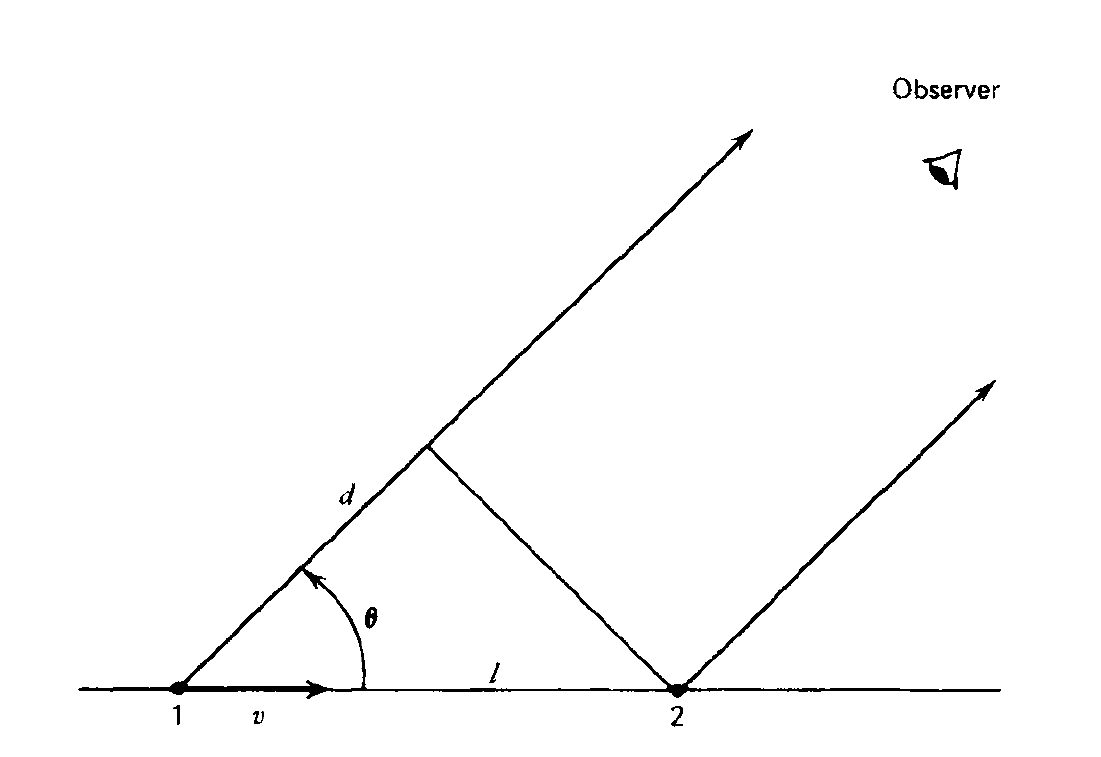
\includegraphics[scale= 0.2]{Figures/RelatDopplerGeometry.png}
 \caption{Γεωμετρία φαινομένου \textlatin{Doppler.} (Εικόνα \cite{1986rpa..book.....R}) }
 \label{fig:lightpathsphere}
 \end{center}
 \end{figure}
Άρα η ισχύς ανά στερεά γωνία  που εκπέμπεται και η ισχύς ανά στερεά γωνία  που λαμβάνεται και καταγράφεται (στο σύστημα $Κ$) θα είναι, δεδομένου ότι $\mu^\prime = \frac{\mu-\beta}{1-\mu \beta}$:
\begin{subequations}
\label{eq:PowerSolAngle}
\begin{align}
\dfrac{dP_e}{d\Omega} = \dfrac{dW}{dt_e d\Omega} = \gamma^3(1+\beta \mu^\prime)^3\dfrac{dW^\prime}{\gamma dt_e^\prime  d\Omega^\prime} = \frac{1}{\gamma^4 (1-\beta\mu)^3}\dfrac{dP_e^\prime}{d\Omega^\prime}   \label{eq:PowerSolAngleA} \\ 
\dfrac{dP_r}{d\Omega} = \dfrac{dW}{dt_r d\Omega} = \gamma^3(1+\beta \mu^\prime)^3\dfrac{dW^\prime}{\gamma (1-\beta \mu) dt_r^\prime  d\Omega^\prime} = \frac{1}{\gamma^4 (1-\beta\mu)^4}\dfrac{dP_r^\prime}{d\Omega^\prime}   \label{eq:PowerSolAngleB} 
\end{align}
\end{subequations}
Η ισχύς ακτινοβολίας που εκπέμπεται ανά στερεά γωνία δίνεται από την εξίσωση \ref{eq:PowerSolAngleA} ενώ η ισχύς ακτινοβολίας ανά στερεά γωνία που παρατηρείται δίνεται από την εξίσωση \ref{eq:PowerSolAngleB}\cite{1986rpa..book.....R}. Οι δύο αυτές σχέσεις, όπως βλέπουμε, διαφοροποιούνται. Όταν μιλάμε για παρατηρήσεις αστροφυσικών αντικειμένων ως ισχύ ακτινοβολίας εννοούμε την παρατηρούμενη- εκτός αν επισημανθεί διαφορετικά.
%============================================================
%============================================================
%============================================================

\section{Βασικές έννοιες ακτινοβολίας}
Για να περιγράψουμε την αλληλεπίδραση ακτινοβολίας με την ύλη χρησιμοποιούμε τρείς βασικές ποσότητες: 
\begin{itemize}
    \item την ειδική ένταση ακτινοβολίας $I_\nu$ που μας δίνει την τοπική ροή ανά μονάδα χρόνου, συχνότητας, επιφάνειας και στερεάς γωνίας στην πηγή 
    \item τον συντελεστή μονοχρωματικής απορρόφησης $\kappa_\nu$  που συνδυάζει όλες τις διαδικασίες απώλειας ενέργειας (απορρόφηση  και σκεδασμό)
    \item τον συντελεστή μονοχρωματικής εκπομπής $j_\nu$ που δίνει την τοπικά εκπεμπόμενη ροή ανά μονάδα όγκου, χρόνου, συχνότητας και στερεάς γωνίας
\end{itemize}      
Οι παραπάνω ποσότητες συνθέτουν την εξίσωση διάδοσης ακτινοβολίας 
\begin{equation}
    \frac{dI_\nu}{ds} = -\kappa_\nu I_\nu+j_\nu
\end{equation}
όπου $ds$ είναι το στοιχείο μήκους, ο πρώτος όρος του δεξιού μέλους περιγράφει την απώλεια ενέργειας λόγω απορρόφησης και ο δεύτερος περιγράφει την παραγωγή ακτινοβολίας από διαδικασίες εκπομπής\cite{netzer_2013}. Ορίζουμε το στοιχείο οπτικού βάθους $d \tau_\nu = \kappa_\nu ds$ και η παραπάνω εξίσωση γίνεται
\begin{equation}
    \frac{dI_\nu}{d\tau_\nu} = -I_\nu+S_\nu
\end{equation}
Η συνάρτηση $S_\nu =j_\nu/\kappa_\nu $ λέγεται συνάρτηση πηγής. Η γενική εξίσωση διάδοσης ακτινοβολίας είναι περίπλοκη και απαιτεί αριθμητικές τεχνικές για την λύση της. Ωστόσο, για περιπτώσεις απλής γεωμετρίας και κατακόρυφης διεύθυνσης η αναλυτική λύση εξάγεται εύκολα\cite{netzer_2013}.
%============================================================
%============================================================
%============================================================

\section{Ακτινοβολία σύγχροτρον}

Σύμφωνα με την σύγχρονη φυσική κατανόηση των ενεργών γαλαξιακάων πυρήνων, θεωρείται ότι το μεγαλύτερο ποσό της συνολικής μη-θερμικής ακτινοβολίας των \textlatin{AGN} οφείλεται σε εκπομπή ακτινοβολίας σύγχροτρον. Η ακτινοβολία σύγχροτρον σχετίζεται με την ραδιοεκπομπή των ενεργών γαλαξιακών πυρήνων.

\subsection*{Εκπομπή ενός ηλεκτρονίου σε μαγνητικό πεδίο}

Για ηλεκτρόνιο ενέργειας $E$ που κινείται σε ομοιογενές μαγνητικό πεδίο $B$ πυκνότητας ενέργειας $u_B = B^2/8\pi$ ο ρυθμός απώλειας ενέργειας $-dE/dt$ είναι ακριβώς η ισχύς $P$ που εκπέμπεται από το ηλεκτρόνιο δίνεται από την σχέση\cite{netzer_2013} 
\begin{equation}
    P = 2\sigma_T c \gamma^2\beta^2u_Bsin^2\alpha
\end{equation}
όπου $\sigma_T$ η διατομή \textlatin{Thomson}, $c$ η ταχύτητα του φωτός στο κενό, $\gamma = E/m_e c^2$ o παράγοντας \textlatin{Lorentz} kai $\beta=v/c$, όπου $v$ η ταχύτητα του ηλεκτρονίου. Ο όρος $sin^2\alpha$ αναπαριστά την διεύθυνση κίνησης, με $\alpha$ την οξεία γωνία που σχηματίζει η διεύθυνση κίνησης με το μαγνητικό πεδίο. Ο μέσος όρος για ισοτροπικές οξείες γωνίες\cite{netzer_2013}
\begin{equation}
    \overline{P} = \frac{4}{3} \sigma_T c \gamma^2\beta^2u_B \label{eq:powerSynch} 
\end{equation}
Η ακτινοβολία από ένα ηλεκτρόνιο εκπέμπεται στην διεύθυνση της κίνησης. Η κατανομή φασματικής ενέργειας (\textlatin{SED}) της ακτινοβολίας αυτής υπολογίζεται λαμβάνοντας υπ>όψιν την γυροσυχνότητα των ηλεκτρονίων γύρω από τις δυναμικές γραμμές του μαγνητικού πεδίου ($\omega_B = eB/\gamma m_e c$) και το μέσο διάστημα μεταξύ παλμών ($2\pi /\omega_B$). Το πλάτος του παλμού υπολογίζεται λαμβάνοντας υπ>όψιν τον σχετικιστικό μετασχηματισμό χρόνου μεταξύ του αδρανειακού συστήματος ηρεμίας του ηλεκτρονίου και το αδρανειακό σύστημα παρατήρησης, έτσι το πλάτος του παλμού είναι ανάλογο του $\gamma^{-3}$. O μετασχηματισμός \textlatin{Fourier} του παλμού, μας δίνει το μέσο εκπεμπόμενο φάσμα ενός ηλεκτρονίου $\overline{P_\nu}(\gamma)$ το οποίο έχει μέγιστο κοντά στο $\gamma \omega_L$, όπου $\omega_L$ η συχνότητα \textlatin{Larmor} με $\omega_L = eB/m_ec$ \cite{netzer_2013}.

\subsection*{Εκπομπή σύγχροτρον από κατανομή ηλεκτρονίων νόμου δύναμης}

Θεωρούμε συλλογή ηλεκτρονίων με κατανομή ενεργειών $n(\gamma)d\gamma$ η οποία μας δίνει το πλήθος των ηλεκτρονίών ανά μονάδα όγκου με ταχύτητες τέτοιες ώστε η τιμή της παραμέτρου $\gamma$ να βρίσκεται στο διάστημα $\gamma - (\gamma +d\gamma)$. Ο συντελεστής εκπομπής των ηλεκτρονίων για όλες τις ενέργειες θα είναι\cite{netzer_2013}
\begin{equation}
    j_\nu =\frac{1}{4\pi} \int_1^\infty \overline{P_\nu}(\gamma) n(\gamma)d\gamma 
\end{equation}
Το παραπάνω ολοκλήρωμα δεν έχει γενική λύση, αφού η κατανομή ενεργειών $n(\gamma)$ μπορεί να πάρει οποιαδήποτε μορφή, όμως υπάρχουν περιπτώσεις όπου η $n(\gamma)$ περιγράφεται ως νόμος δύναμης στις ενέργειες $n(\gamma )d\gamma = n_0 \gamma^{ − p} d\gamma $. Επίσης, κάνοντας την παραδοχή ότι κάθε ακτινοβολία έχει ένα μέγιστο κοντά σε μία χαρακτηριστική συχνότητα $\gamma^2 \nu_L$, όπου $\nu_L$ η συχνότητα \textlatin{Larmor}, προκύπτει η αναλυτική μορφή του συντελεστή εκπομπής\cite{netzer_2013}
\begin{equation}
    4\pi j_\nu =\frac{2}{3} \sigma_T n_0 u_B \nu_L^{-1} \Big( \frac{\nu}{\nu_L} \Big)^{-\frac{p-1}{2}}
\end{equation}
Η μονοχρωματική φωτεινότητα $L_\nu$ οπτικά αραιού μέσου που εκπέμπει ακτινοβολία σύνχροτρον προκύπτει ολοκληρώνοντας τον παράγοντα εκπομπής στον όγκο της πηγής\cite{netzer_2013}
\begin{equation}
    L_\nu =\int_V j_\nu dV  \propto \nu^{-\frac{p-1}{2}} \label{eq:LumiSynch}
\end{equation}
Η λογαριθμική κλίση προσαρμόζεται στο παρατηρούμενο φάσμα πολλών \textlatin{AGN} στα ραδιοκύματα, στο οπτικό/υπεριώδες και στις ακτίνες Χ. 

\subsection*{Αυτοαπορρόφηση σύγχροτρον}

Η εκπομπή σύγχροτρον συνοδεύεται από απορρόφηση, κατά την οποία ένα φωτόνιο αλληλεπιδρά με φορτίο εντός του μαγνητικού πεδίου και απορροφάται αποδίδοντας όλη του την ενέργεια στο φορτίο. Μία άλλη διαδικασία που μπορεί να συμβεί είναι η εξαναγκασμένη εκπομπή ή αρνητική απορρόφηση, κατά την οποία ένα σωματίδιο εκπέμπει ισχυρότερα σε μία συχνότητα\cite{1986rpa..book.....R}. Ο συντελεστής αυτοαπορρόφησης σύγχροτρον προκύπτει\cite{1986rpa..book.....R} $\alpha_\nu \propto \nu^{-(p+4)/2} $.
%============================================================
%============================================================
%============================================================

\section{Σκεδασμός \textlatin{Compton}}

Η αλληλεπίδραση ηλεκτρόνιου με δέσμη φωτονίου περιγράφεται από τον σκεδασμό \textlatin{Compton}. Για στατικά ή αργά κινούμενα ηλεκτρόνια, χρησιμοποιούμε τις σχέσεις διατήρησης ενέργειας και ορμής για να εξάγουμε τις σχέσεις μεταξύ των συχνοτήτων της προσπίπτουσας δέσμης φωτονίων ($\nu^\prime$) και της σκεδαζόμενης δέσμης φωτονίων ($\nu$). Αν $\vec{n_\nu}$ και $\vec{n_{\nu^\prime}}$ μοναδιαία διανύσματα στις διευθύνσεις των δέσμων αυτών και γωνία $\theta$ τέτοια ώστε $cos \theta = \vec{n_\nu} \cdot \vec{n_{\nu^\prime}} $, τότε\cite{netzer_2013}
\begin{equation}
    \nu =\dfrac{ m_e c^2\; \nu^\prime }  { m_e c^2+ h \nu^\prime(1-cos\theta) } \label{eq:ComptonWavelength} 
\end{equation}
Για μη σχετικιστικά ηλεκτρόνια η ενεργός διατομή της διαδικασίας αυτής δίνεται από την εξίσωση\cite{netzer_2013}
\begin{equation}
    \frac{d\sigma}{d\Omega} =\frac{1}{2}  r_e^2 (1+cos^2 \theta)
\end{equation}
όπου $r_e = e^2/m_e c^2$ η ακτίνα ηλεκτρονίου στην κλασσική φυσική. Η ολοκλήρωση της παραπάνω σχέσης σε όλες τις γωνίες μας δίνει την ενεργό διατομή \textlatin{Thomson} $\sigma_T$.\\
Στο όριο των υψηλών ενεργειών χρησιμοποιούμε την ενεργό διατομή \textlatin{Klein–Nishina} $\sigma_{KN}$ για την έκφραση της οποίας χρησιμοποιούμε την ποσότητα $\epsilon = h\nu/m_e c^2$ οπότε η προσέγγιση γίνεται\cite{netzer_2013} 
\begin{equation}
    \sigma_{KN} =\begin{cases} \sim \sigma_T (1-2\epsilon)\;\;\;\;\;\;\;\; \;\;\;\;\;\;\; \mbox{gia}\;\; \epsilon<<1 
    \\ \;\\ 
    \sim \frac{3}{8}\frac{\sigma_T}{\epsilon} \Big(ln2\epsilon +\frac{1}{2} \Big) \;\;\;\;\;\;\;\; \mbox{gia}\;\; \epsilon>>1 \end{cases}
\end{equation}

\subsection*{Αντίστροφος σκεδασμός \textlatin{Compton}}

Ο αντίστροφος σκεδασμός \textlatin{Compton} είναι η διαδικασία κατά την οποία (σχετικιστικά) κινούμενο ηλεκτρόνιο σκεδάζει φωτόνιο, με αποτέλεσμα να του μεταφέρει μέρος της ενέργειάς του. Μας ενδιαφέρει η εξίσωση για την μέση ισχύ που εκπέμπεται λόγω αντιστρόφου σκεδασμού \textlatin{Compton} για κατανομή φωτονίων που σκεδάζονται από μια δεδομένη ισοτροπική κατανομή κινούμενων ηλεκτρονίων. Θεωρούμε αριθμητική πυκνότητα $n_{ph}$ δέσμης φωτονίων με μέση ενέργεια πριν την σκέδαση $h\overline{\nu_0}$. Η ενεργειακή πυκνότητα των φωτονίων αυτών θα είναι $u_{rad} = n_{ph} h\overline{\nu_0}$. Η μέση ενέργεια μετά την σκέδαση $h\overline{\nu}$, όπως φαίνεται από την σχέση \ref{eq:ComptonWavelength}, είναι μεγαλύτερη από αυτήν πριν την σκέδαση κατά παράγοντα τάξης $\gamma^2$. Στο σύστημα ηρεμίας του ηλεκτρονίου η διαδικασία αυτή μοιάζει με σκεδασμό \textlatin{Thomson} με μέση ισχύ ακτινοβολίας που δίνεται από την σχέση $\overline{P} = \sigma_T c u_{rad} $. Έτσι, για την απλή εκτίμηση $L_\nu \propto \nu^{-(p-1)/2}$, sto αδρανειακό σύστημα παρατήρησης η μέση εκπεμπόμενη ισχύς είναι $ \overline{P} = \gamma^2 \sigma_T c u_{rad} $. Ενώ ο ακριβής υπολογισμός της μέσης εκπεμπόμενης ισχύος λαμβάνει υπ>όψιν την γωνία σκέδασης και τον μετασχηματισμό της από το σύστημα ηρεμίας του ηλεκτρονίου στο σύστημα παρατήρησης και η τελική σχέση που προκύπτει είναι\cite{netzer_2013}
\begin{equation}
    \overline{P} = \frac{4}{3} \sigma_T c \gamma^2 \beta^2 u_{rad} \label{eq:powerIC} 
\end{equation}
Η έκφραση μέσης ακτινοβολούμενης ισχύος λόγω αντιστρόφου \textlatin{Compton} (εξίσωση \ref{eq:powerIC}) δεν διαφέρει σημαντικά από την έκφραση μέσης ακτινοβολούμενης ισχύος ακτινοβολίας σύγχροτρον (εξίσωση \ref{eq:powerSynch}). Η μόνη διαφορά έγκειται στο ότι η ενεργειακή πυκνότητα του μαγνητικού πεδίου $u_B$ της εξίσωσης για την ακτινοβολία σύγχροτρον αντικαθίσταται στην αντίστοιχη σχέση αντιστρόφου \textlatin{Compton} με την ενεργειακή πυκνότητα του πεδίου ακτινοβολίας $u_{rad}$. Οπότε, θεωρώντας ότι αυτές οι δύο διαδικασίες λαμβάνουν χώρα στον ίδιο όγκο, η μέση ισχύς ακτινοβολίας τους θα είναι $u_B/u_{rad}$. Η κατανομή ενέργειας των σχετικιστικών ηλεκτρονίων στο ίδιο αυτόν όγκο δίνεται από την ίδια συνάρτηση νόμου δύναμης που χρησιμοποιήθηκε στην περίπτωση της ακτινοβολίας σύγχροτρον $n(\gamma) \propto \gamma^{-p}$ με αποτέλεσμα να έχουμε την ίδια εξάρτηση της μονοχρωματικής φωτεινότητας από την παράμετρο $p$\cite{netzer_2013} 
\begin{equation}
    L_\nu \propto \nu^{-\frac{p-1}{2}} \label{eq:LumiIC} 
\end{equation}

\subsection*{Μηχανισμός \textlatin{Synchrotron-Self-Compton}}

Σε συμπαγή πηγή ακτινοβολίας σύγχροτρον τα εκπεμπόμενα φωτόνια μπορούν μέσω αντιστρόφου \textlatin{Compton} να σκεδαστούν από τα ίδια σχετικιστικά ηλεκτρόνια που εκπέμπουν την ακτινοβολία σύγχροτρον. Η διαδικασία αυτή αυξάνει σημαντικά την ενέργεια του φωτονίου και η ακτινοβολία που προκύπτει ονομάζεται εκπομπή \textlatin{Synchrotron-Self-Compton (SSC)}. Ο μηχανισμός αυτός αφορά ακτινοβολίες πολύ υψηλών ενεργειών (ακτίνες $\gamma$ από $>100$ \textlatin{MeV} έως τάξης \textlatin{ΤeV}) από ραδιογαλαξίες, \textlatin{pulsar} ή υπερκαινοφανείς. Η ροή που εκπέμπεται από την διαδικασία αυτή υπολογίζεται ολοκληρώνοντας το φάσμα της ακτινοβολίας σύγχροτρον και την κατανομή ενέργειας του πεδίου ηλεκτρονίων. Σε καλή προσέγγιση ο φασματικός δείκτης (λογαριθμική κλίση) που προκύπτει είναι συμβατός με τον φασματικό δέικτη της πηγής σύγχροτρον.\\
Η διαδικασία \textlatin{Synchrotron-Self-Compton} μπορεί να επαναλαμβάνεται στην ίδια πηγή από περεταίρω σκέδαση των παραγόμενων φωτονίων, με αποτέλεσμα να αυξάνεται η ενέρεγια των φωτονίων κατά παράγοντα $\gamma^2$. Το φυσικό όριο της διαδικασίας αυτής έρχεται όταν η ενέργεια σκεδαζόμενου φωτονίου αγγίζει το φάσμα των ακτίνων $\gamma$ και η συνθήκη $h \nu_\gamma \ll m_e C^2 $ για μη-ανάκρουση \textlatin{Compton} των ηλεκτρονίων παύει να ισχύει, στο όριο αυτό η πυκνότητα ακτινοβολίας ελαττώνεται γρήγορα\cite{netzer_2013}.\\
Ο μηχανισμός αυτός παράγει την ακτινοβολία Χ που παρατηρούμε σε ενεργούς γαλαξιακούς πυρήνες και παράγεται από διαδικασίες που σχετίζονται άμεσα με την προσάυξηση μάζας στην κεντρική μελανή οπή.

%============================================================
%============================================================
%============================================================

\section{Ακτινοβολία πέδης (\textlatin{bremsstrahlung})}

Η ακτινοβολία λόγω επιτάχυνσης φορτίου σε πεδίο \textlatin{Coulomb} που παράγει άλλο φορτίο λέγεται ακτινοβολία πέδης, ή \textlatin{bremsstrahlung}, ή εκπομπή \textlatin{free-free}.\\
H ακτινοβολία \textlatin{bremsstrahlung} από σύγκρουση όμοιων σωαμτιδίων (π.χ. ηλεκτρονίου-ηλεκτρονίου) δίνει μηδενική ένταση ακτινοβολίας στην προσέγγυση διπόλου, οπότε μας ενδιαφέρει η σύγκρουση διαφορετικών σωματιδίων. Ακτινοβολία \textlatin{bremsstrahlung} μελετάμε κυρίως από ζέυγος ηλεκτρονίου-ιόντος, αφού η σχετικές επιταχύνσεις τους είναι αντιστρόφως ανάλογες των μαζών και τα φορτία τους σχεδόν ίσα. Η μάζα του ιόντος είναι κατά πολλύ μεγαλύτερη αυτής του ηλεκτρονίου, οπότε μπορούμε να μελετάμε το ηλεκτρόνιο σαν να κινείται σε σταθερό πεδίο  \textlatin{Coulomb} του ιόντος\cite{1986rpa..book.....R}.\\
Η ακτινοβολία \textlatin{bremsstrahlung} είναι τεχνικά θερμική ακτινοβολία, όμως το σχήμα του φάσματος διαφέρει από αυτό μελανού σώματος. Η εκπομπή ακτινοβολίας \textlatin{bremsstrahlung} από επιτάχυνση ηλεκτρονίου στο πεδίο ιόντος φορτίου $Z$ με αριθμητική πυκνότητα $N_i$ περιγράφεται από τον συντελεστή εκπομπής\cite{netzer_2013}
\begin{equation}
    4\pi j_\nu = 6.8\times 10^{-38} Z^2 T_e^{-1/2}N_e N_i g_{ff}(\nu, T_e,Z)e^{-h\nu/kT_e} 
\end{equation}
όπου $N_e$ kai $T_e$ η αριθμητική πυκνότητα και η θερμοκτρασία ηλεκτρονίων και $g_{ff}(\nu, T_e,Z)$ είναι η μέση τιμή του παράγοντα \textlatin{Gaunt} για όλες τις ταχύτητες- ο οποίος διορθώνει για κβαντικά φαινόμενα. Ο παράγοντας αυτός είναι τάξης $1$ και μπορεί να αλλάξει ελαφρώς με την συχνότητα. Για ενέργειες ακτίνων Χ έχουμε $g_{ff} \propto \nu^{-0.1}$. H ακτινοβολία \textlatin{bremsstrahlung} εκτείνεται σε πολλές διαφορετικές ενέργειες και το φάσμα της έχει μορφή νόμου δύναμης με πολύ μικρό φασματικό δέικτη (σχεδόν επίπεδο φάσμα)\cite{netzer_2013} σχετίζεται με εκπομπή ακτίνων Χ από σμήνη γαλαξιών στο συνεχές, αλλά και με εκπομπή γραμμών στα ραδιοκύματα από ιονισμένο υδρογόνο.\\
Ολοκληρώνοντας την εκπομπή σε όλες τις συχνότητες καταλήγουμε στην ολική ενέργεια ανά μονάδα ανά μονάδα όγκου ανά δευτερόλεπτο $C_{ff}$, η ποσότητα αυτή αναπαριστά επίσης τον ρυθμό ψύξης λόγω ακτινοβολίας πέδης. Η ολοκλήρωση αυτή δίνει\cite{netzer_2013}
\begin{equation}
    C_{ff} = 1.42\times 10^{-27} Z^2 T_e^{-1/2}N_e N_i g_{ff} \; erg \;s^{−1}\; cm^{−3}
\end{equation}
όπου η ποσότητα $g_{ff}$ εκφράζει την μέση τιμή για συχνότητες της μέσης τιμής για ταχύτητες του παράγοντα \textlatin{Gaunt} και απ'ιρνει τιμές $1.1-1.5$ \cite{netzer_2013}.
%============================================================
%============================================================
%============================================================ 

\section{Αστροφυσικές παρατηρήσεις \textlatin{AGN} στις ακτίνες Χ}
% Η πλεον ισχυση γραμμη εκπομπης στις ακτινες, Fe-Ka, εμφανιοζεται (μερικες φορες) φαρδυα λογω βρατυρικων φαινομενων και οχι επειδη προερχεται απο περιστρεφομενα νεφη γυρω απο τη μελανη οπη.
\begin{figure*}
 \begin{center}
 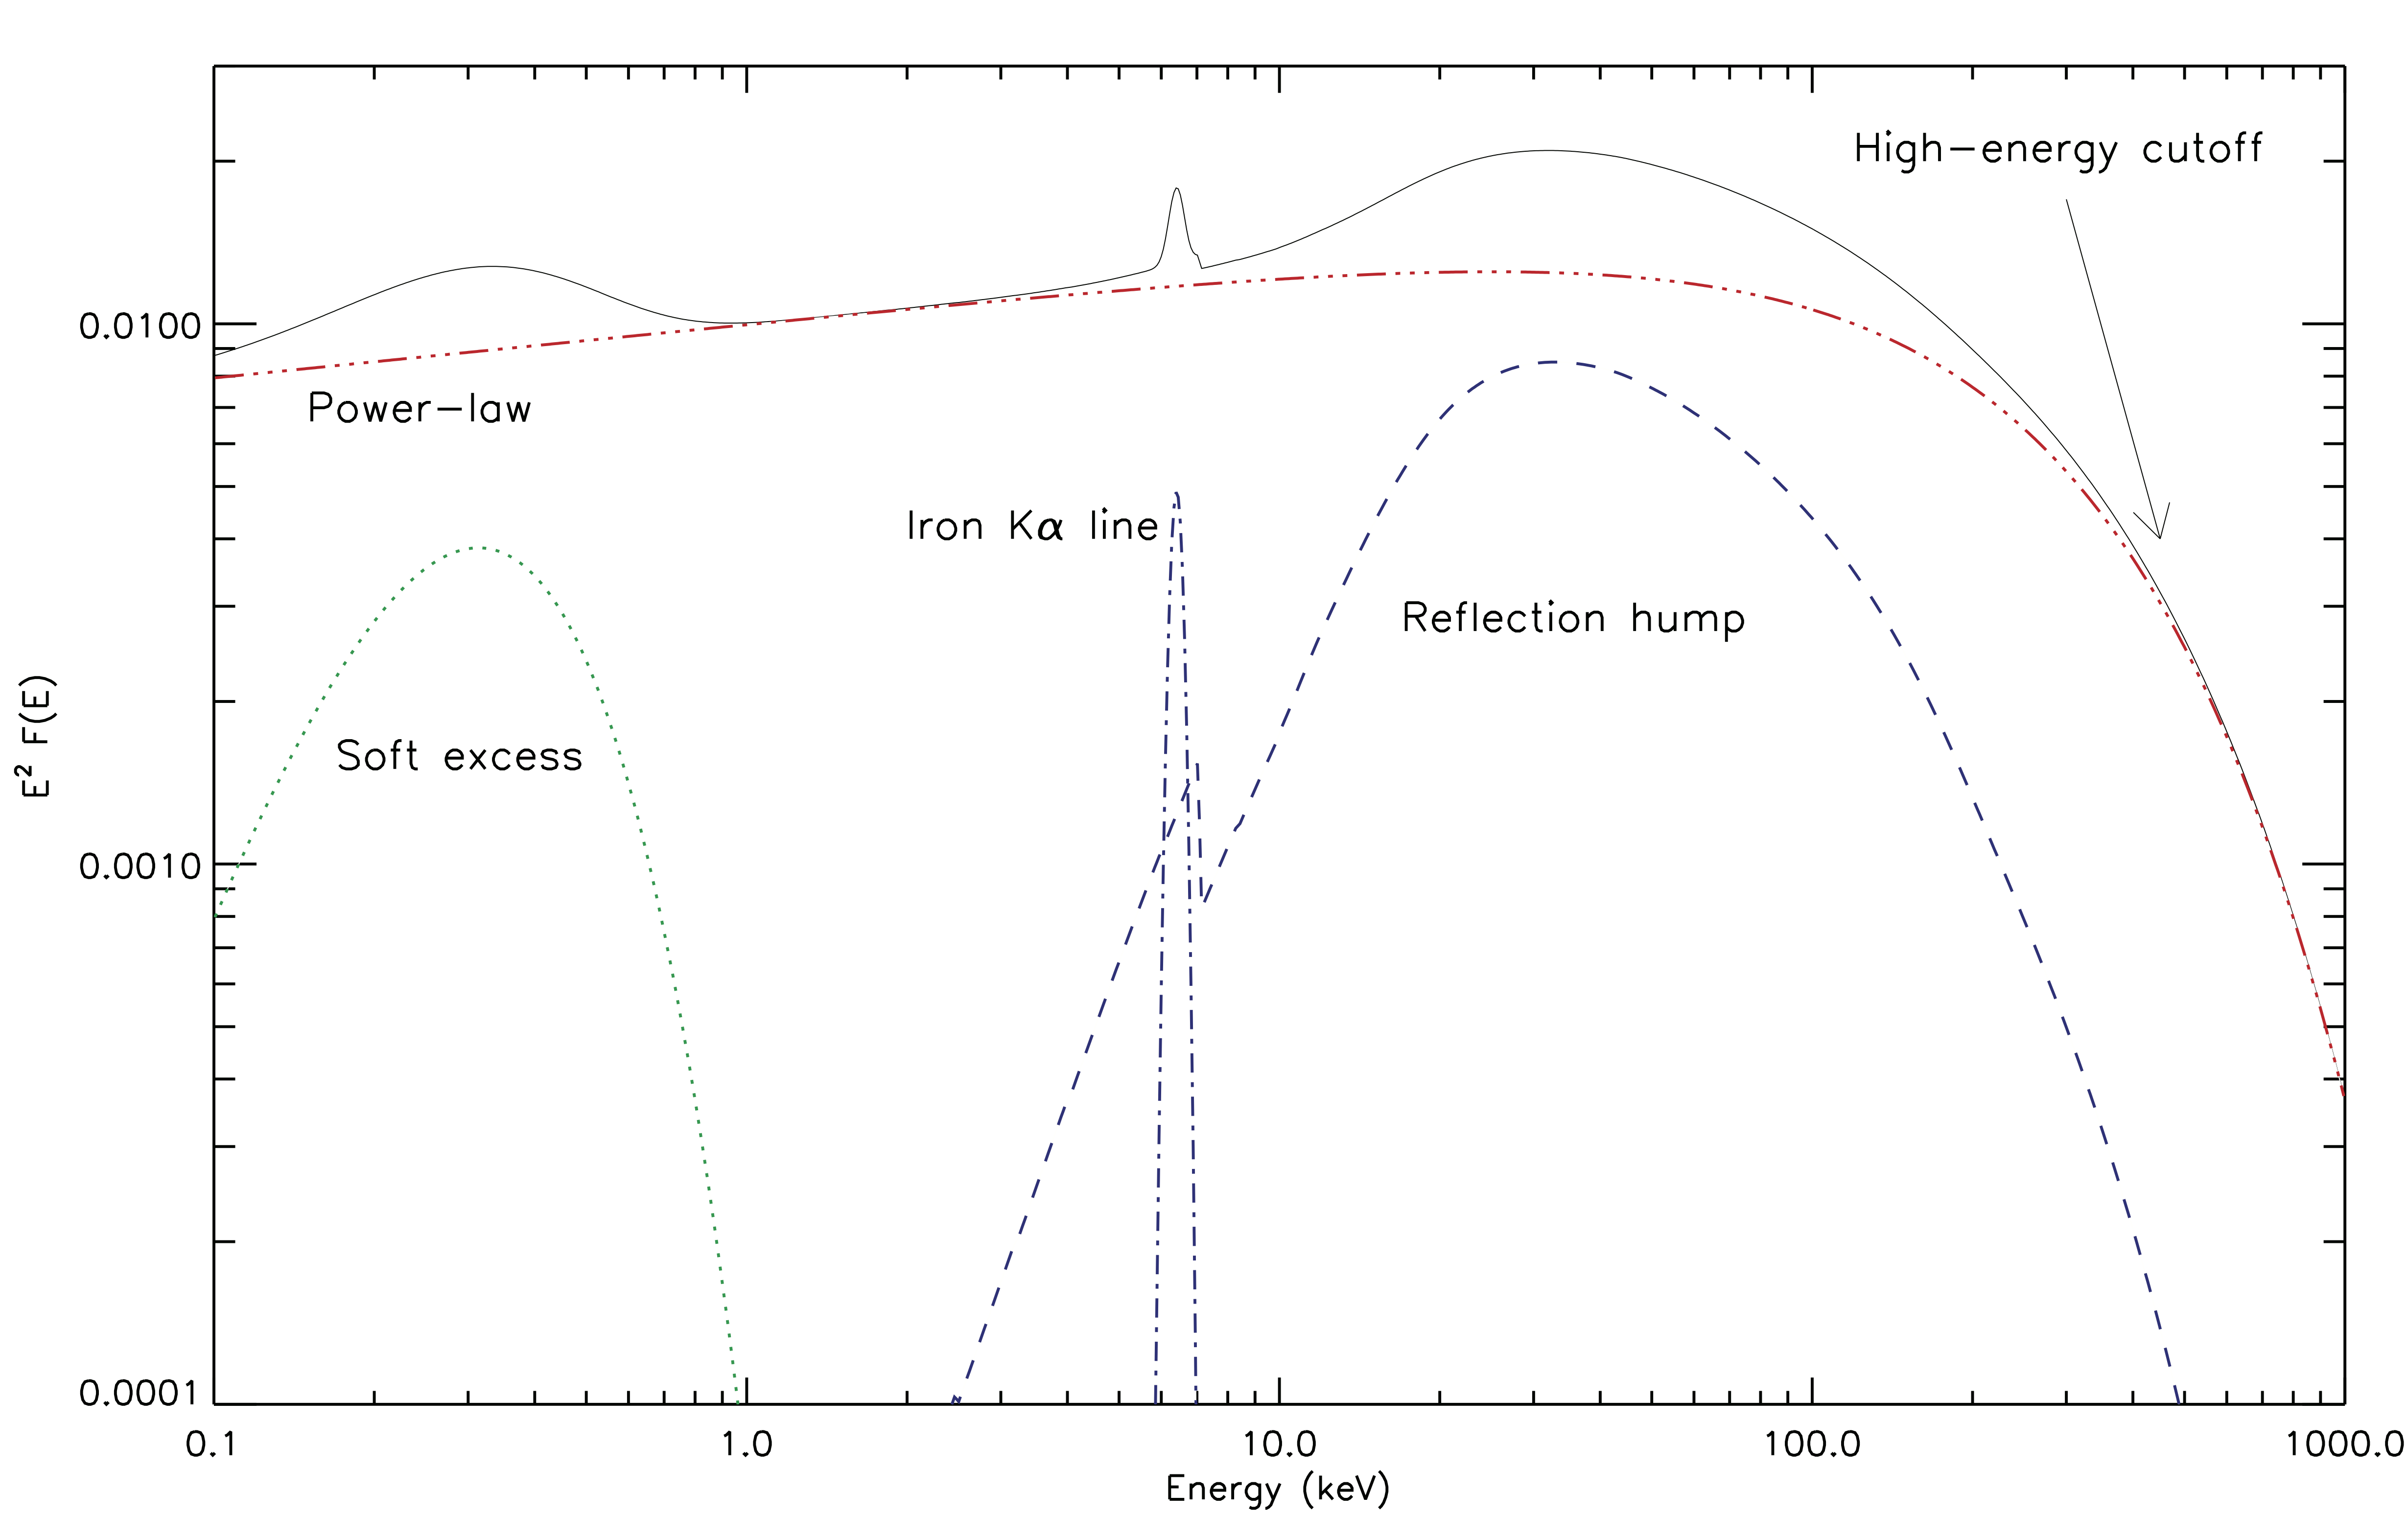
\includegraphics[width=0.9\linewidth]{Figures/X-ray_spectrum_AGN_hres.jpg}
 \caption{Τυπικό φάσμα \textlatin{AGN} τύπου 1 σε ενέργειες $0.1-1000$ \textlatin{keV} (Εικόνα από \textlatin{Ricci et al. 2011})} \label{fig:agnspec}
 \end{center}
\end{figure*}
Τα φάσματα των \textlatin{AGN} στις ακτίνες Χ είναι σχετικά ομοιογενή και περιγράφονται καλά με νόμο δύναμης μέσα σε ένα εύρος φασματικών δεικτών. Η γραμμή εκπομπής σιδήρου \textlatin{Fe K$_\alpha$} και η κύρτωση στα $\sim 10$ \textlatin{keV} θεωρείται ότι ωφείλονται σε ψυχρή ύλη (εικόνα \ref{fig:agnspec}). Μέρος της ψυχρής αυτής ύλης πρέπει να βρίσκεται κοντά στην περιοχή παραγωγής ακτίνων Χ, όπως υποδεικνύει η μικρή χρονική καθυστέρηση μεταξύ της μεταβολής στην γραμμή σε σχέση με την μεταβολή στο συνεχές. Η φυσική εξήγηση για την δομή είναι οπτικά πυκνός δίσκος προσάυξησης η εκπομπή από τον οποίο μπορεί να εξηγήσει το παρατηρούμενο φάσμα\cite{1991ApJ}.
\begin{figure*}
 \begin{center}
 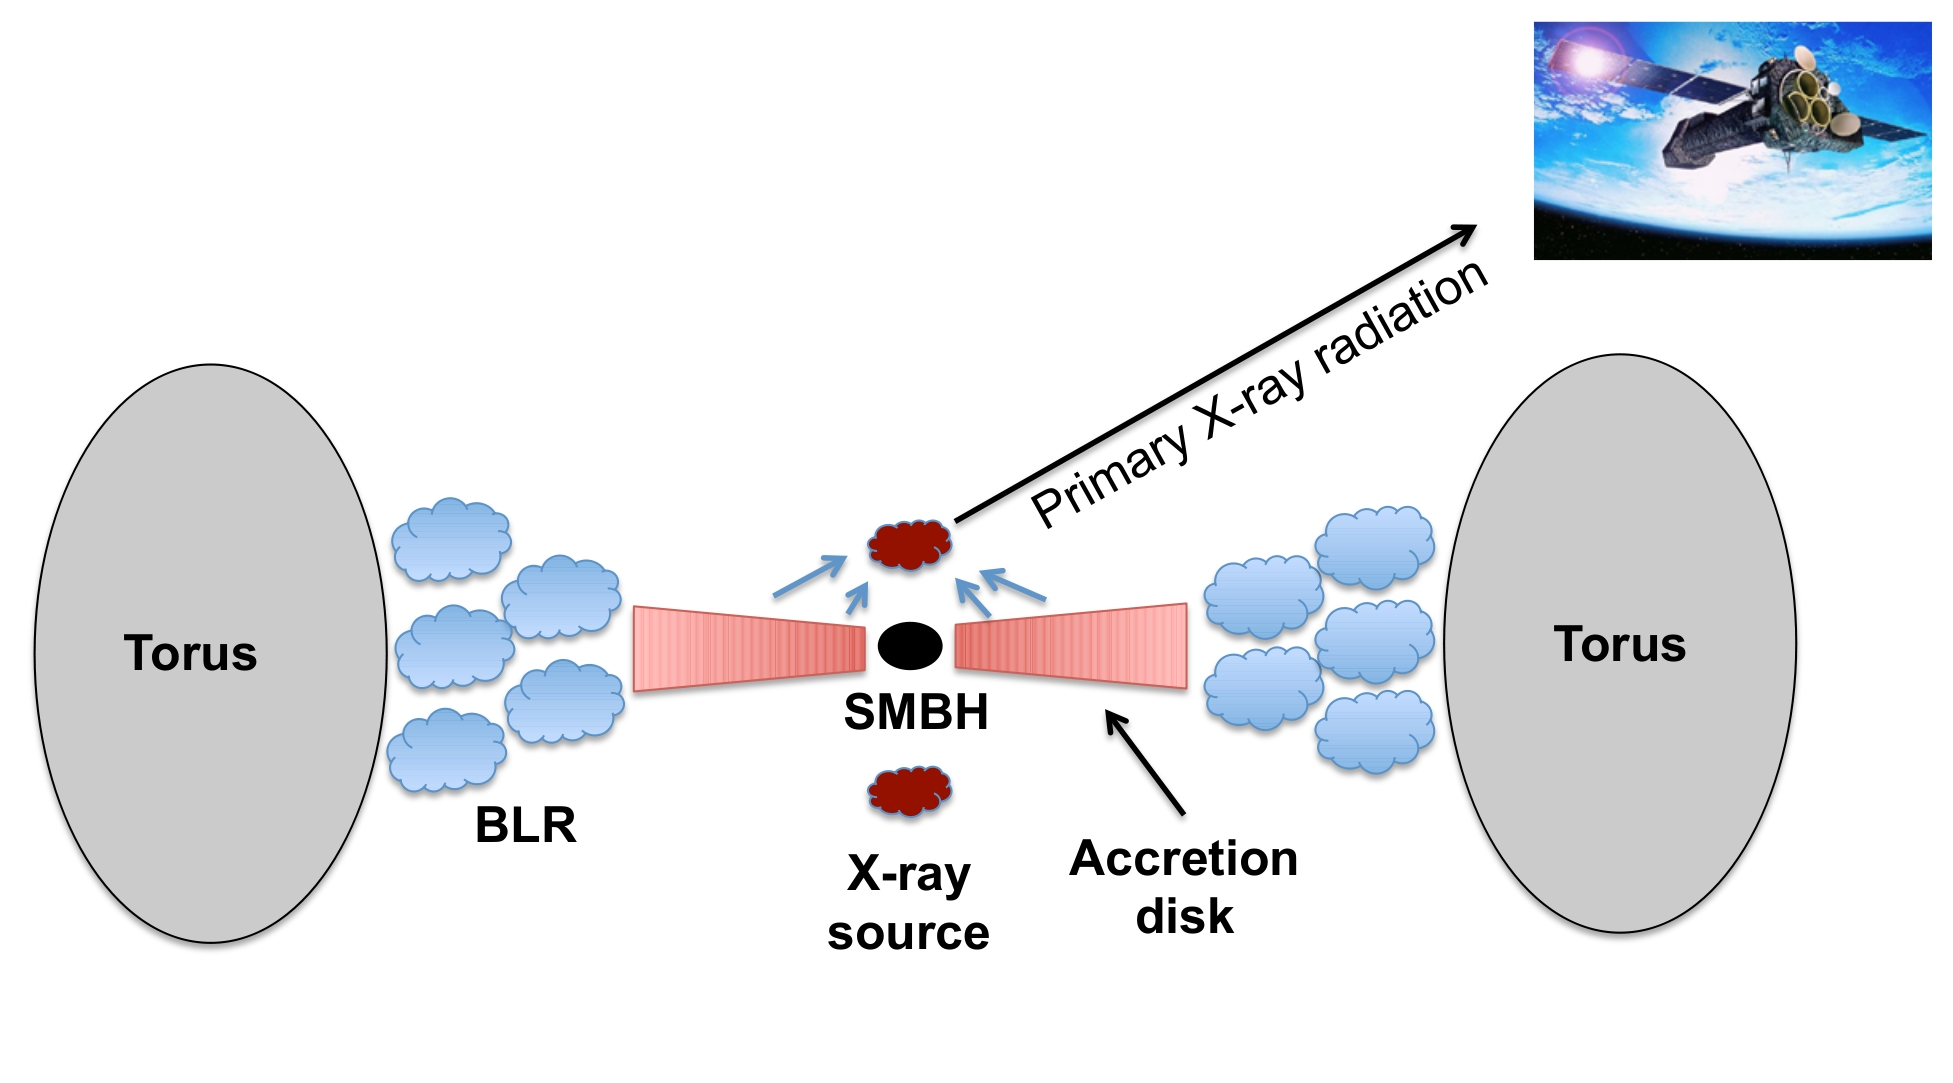
\includegraphics[width=0.7\linewidth]{Figures/X_ray_primary_1.jpg}
 
 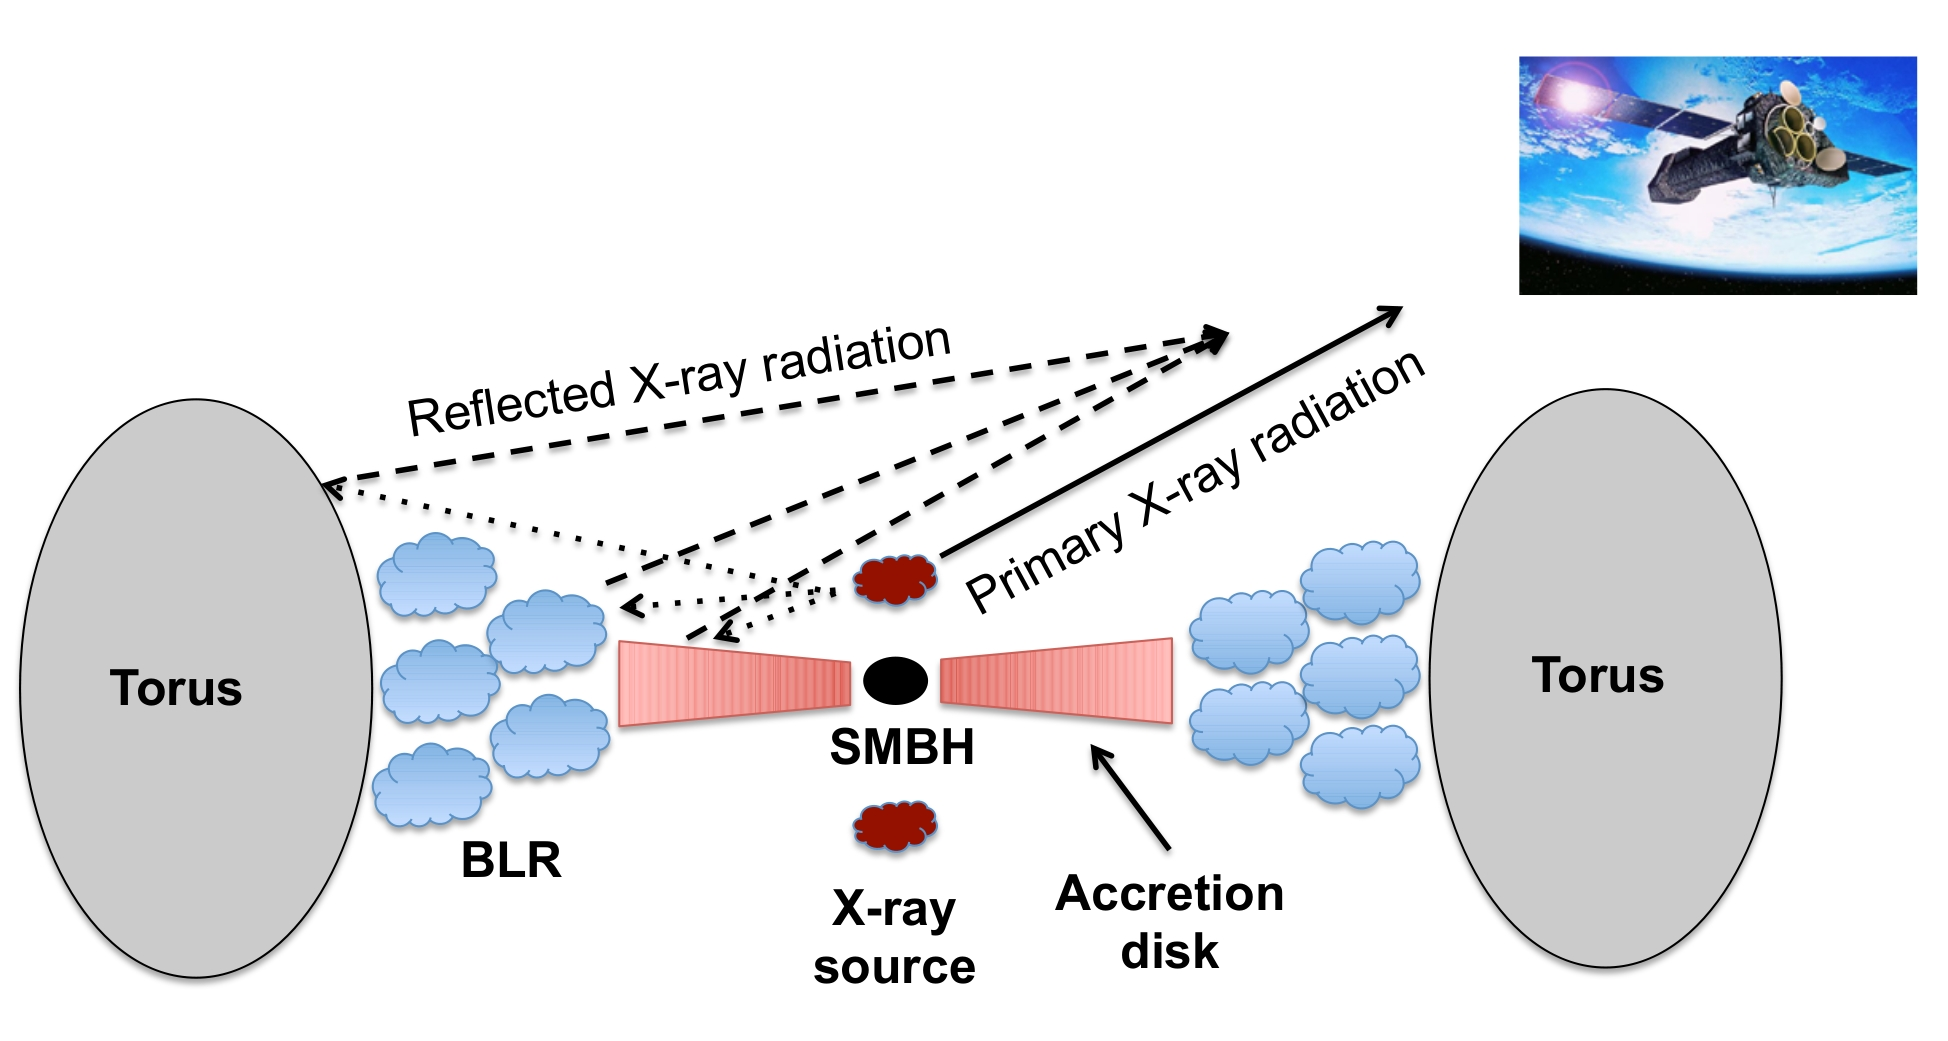
\includegraphics[width=0.7\linewidth]{Figures/X_ray_refl_1.jpg}
 \caption{Σχηματική αναπαράσταση παραγωγής ακτίνων Χ σε \textlatin{AGN}- η περιοχή από την οποία προέρχονται οι ακτίνες Χ είναι πιθανότατα ένα στέμμα πλάσματος ηλεκτρονίων. Πάνω: διαδρομή φωτός πρωτογενών ακτίνων Χ. Κάτω: διαδρομή φωτός δευτερογενών ακτίνων Χ (Εικόνα από \textlatin{www.isdc.unige.ch/$\sim$ricci})} \label{fig:xray_primary}
 \end{center}
\end{figure*}
Η αιτία που παράγει την μορφή νόμου δύναμης των φασμάτων των \textlatin{AGN} δεν είναι ξεκάθαρη. 
% Έχει εξετασθεί μοντέλο κατά το οποία κάποιος μηχανισμός εισάγει υψηλοενεργειακά φωτόνια που μετατρέπονται σε ζεύγος ηλεκτρονίου-ποζιτρονίου (παρουσία πυρήνα) και εκκινούν σωματιδιακούς καταιονισμούς που έχουν ως αποτέλεσμα διαδικασίες σκεδασμών \textlatin{Compton}. Άλλα μοντέλα προτείνουν θερμική ακτινοβολία \textlatin{bremsstrahlung}, η οποία θεωρείται ο μηχανισμός που παράγει την μεγαλύτερη εκπομπή ακτίνων Χ σε παρατηρήσεις σμηνών γαλαξιών και έχει φάσμα συμβατό με νόμο δύναμης\cite{1991ApJ}.

Το κυρίαρχο μοντέλο βασίζεται σε αντίστροφους σκεδασμούς \textlatin{Compton} μαλακών φωτονίων που ψύχουν θερμό αέριο ηλεκτρονίων, αυτό μας δίνει την εικόνα θερμού στέμματος θερμικών ηλεκτρονίων υψηλής ενέργειας (T$_{electron} \sim 10^9$  K) που ακτινοβολείται από φωτόνια οπτικού/υπεριώδους που παράγονται στον δίσκο και ψύχεται μέσω αντίστροφης σκέδασης \textlatin{Compton} κατά την οποία τα προσπίπτοντα φωτόνια αυξάνουν την ενέργειά τους και σκεδάζονται ως ακτινοβολία Χ (εικόνα \ref{fig:xray_primary}). Η αντίστροφη σκέδαση \textlatin{Compton} παράγει φυσικά φάσμα νόμου δύναμης (εξίσωση \ref{eq:LumiIC}) και ο παρατηρούμενος φασματικός δείκτης είναι $\Gamma \sim 1.8-2.0$ \cite{1991ApJ}.\\    
Το μοντέλο αυτό εξηγεί ότι η αποκοπή στην μορφή νόμου δύναμης (\textlatin{broken power law}) οφείλεται στο γεγονός ότι το στέμμα πλάσματος ηλεκτρονίων είναι θερμικό- δηλαδή τα ηλεκτόνια ακολουθούν κατανομή \textlatin{Maxwell}. Το ενεργειακό κατώφλι της δίδυμης γένεσης (παραγωγής ζεύγους ηλεκτρονίου-ποζιτρονίου από φωτόνιο παρουσία πυρήνα) είναι $\sim 511$ \textlatin{keV}, οπότε το στέμμα πλάσματος έχει όριο θερμοκρασίας. Συγκεκριμένα, το στέμμα δεν μπορεί να σκεδάζει φωτόνια με ενέργεια πάνω από  $\sim 150$ \textlatin{keV} πολύ αποδοτικά- σε μεγαλύτερες ενέργειες αρχίζουν διαδικασίες δίδυμης γένεσης- έτσι έχουμε εκθετική αποκοπή στην ροή οποία συσχετίζεται με την θερμοκρασία του στέμματος. Οι ιδιότητες του στέμματος είναι χαοτικές και δεν μπορούν να υπολογιστούν από πρώτες αρχές\cite{Brandt}. \\
Μέρος της πρωταρχικής εκπομπής ακτίνων Χ που προκύπτει από αντίστροφο σκεδασμό \textlatin{Compton} προσπίπτει στον τόρο μοριακού αερίου, στην περιοχή εκπομπής διευρυμένων φασματικών γραμμών \textlatin{(Broad Line Region)} ή ακόμα και στον ίδιο τον δίσκο προσάυξησης (σχηματικά στην εικόνα \ref{fig:xray_primary}) και επανεκπέμπεται. Η επανεκπεμπόμενη ακτινοβολία είναι υπεύθυνη για την κύρτωση του φάσματος στις ενέργειες $\sim 30-40$ \textlatin{keV} (σχήμα \ref{fig:agnspec}) και την γραμμή εκπομπής σηδήρου \textlatin{Fe K$_\alpha$} στην ενέργεια $\sim 6.4 $ \textlatin{keV}. Η κύρτωση στα $\sim 30-40$ \textlatin{keV} σημειώνεται μόνο όταν το υλικό πρόσπτωσης είναι πυκνό (με πυκνότητα στήλης Ν$_{Η} >  1.5 \times  10^{24}$ \textlatin{cm}$^{-2}$ - η τιμή του ορίου αυτού αντιστοιχεί στο οπτικό βάθος για την σκέδαση \textlatin{Compton}), ενώ η γραμμή εκπομπής σηδήρου \textlatin{Fe $K_\alpha$} μπορεί να παραχθεί και σε αραιή ύλη και θεωρείται υπέρθεση εκπομπής μίας διευρυμένης γραμμής και μίας στενής γραμμής που υποδηλώνουν εκπομπή από μία εσωτερική περιοχή του συστήματος προσάυξησης (η διευρυμένη γραμμή- π.χ. προέρχεται από τον ίδιο τον δίσκο) και εκπομπή από μία μακρυνότερη περιοχή (η στενότερη γραμμή- π.χ. προέρχεται από τον τόρο ή την \textlatin{BLR}). Η διεύρυνση της γραμμής αυτής οφείλεται σε βαρυτικά φαινόμενα που είναι πιο έντονα στην περιοχή κοντά στην κεντρική μάζα.\\
Αρκετά φάσματα \textlatin{AGN} παρουσιάζουν πλεόνασμα ισχύος ακτινοβολίας που κυρτώνει ελαφρά τον νόμο δύναμης στα $\sim 2 $ \textlatin{keV} (σχήμα \ref{fig:agnspec}). Για τους \textlatin{AGN} τύπου 1 έχουν διατυπωθεί αρκετές πιθανές αιτίες για το πλεόνασμα μαλακών ακτίνων Χ όπως: ανάκλαση από ιονισμένο δίσκο, τοπική απορρόφηση από ιονισμένο άνεμο ή ύπαρξη ενός δεύτερου ψυχρότερου στέμματος. Στους \textlatin{AGN} τύπου 2 η περιοχή απορρόφησης επηρεάζει το παρατηρούμενο φάσμα ακτίνων Χ καθώς λαμβάνουν χώρα διαδικασίες όπως φωτοηλεκτρική απορρόφηση και σκεδασμός \textlatin{Compton}. Η φωτοηλεκτρική απορρόφηση γίνεται αισθητή για υλικό πυκνότητας στήλης N$_{H} \sim 10^{21}$ \textlatin{cm}$^{-2}$ εξαρτάται από την ενέργεια επηρεάζοντας τις μαλακές ακτίνες Χ περισσότερο ενώ δεν παίζει σημαντικό ρόλο για ακτινοβολία ενέργειας $> 10$ \textlatin{keV} για πυκνότητα στήλης N$_{H}<  10^{24}$ \textlatin{cm}$^{-2}$. Ο σκεδασμός \textlatin{Compton} γίνεται σημαντικός για υλικό απορρόφησης πυκνότητας N$_{H} \sim  10^{24}$ \textlatin{cm}$^{-2}$.

\section{\textlatin{XMM-Newton}}

Το διαστημικό παρατηρητήριο \textlatin{ΧΜΜ (X-ray Multi Mirror)} εκτοξεύθηκε τον Δεκέμβρη του 1999 και έχει τρία τηλεσκόπια ακτίνων Χ τύπου \textlatin{Wolter} τύπου 1 με διαφορετικούς ανιχνευτές ακτίνων Χ στο εστιακό τους κέντρο και ένα τηλεσκόπιο για οπτικό/υπεριώδες.

\subsection{Δομή τηλεσκοπίων ακτίνων Χ}

Η εστίαση των ακτίνων Χ δεν γίνεται με το ίδιο τρόπο όπως π.χ. στο οπτικό, καθώς οι ακτίνες Χ έχουν τόσο μικρό μήκος κύματος ώστε τείνουν να διαπερνούν τα κάτοπτρα για γωνία πρόσπτωσης (\textlatin{angle of incidence}) σχετικά μεγάλή\footnote{Εδώ όταν μιλάμε για γωνία πρόσπτωσης, θα εννοούμε την οξεία γωνία που σχηματίζει η δέσμη με την επιφάνεια πρόσπτωσης- και όχι με την κατακόρυφο σε αυτήν.}. Έτσι η τυπική δομή φακών και κατόπτρων που χρησιμοποιούνται για παρατηρήσεις στο οπτικό δεν χρησιμοποιούνται στην αστρονομία ακτίνων Χ. Όμως, για πολύ μικρές γωνίες πρόσπτωσης δηλαδή σχεδόν εφαπτομενική στην επιφάνεια πρόσπτωση (\textlatin{grazing incidence}) μια δέσμη ακτίνων Χ ανακλάται και συμπεριφέρεται όπως το οπτικό- όπως φαίνεται σχηματικά στο σχήμα \ref{fig:grazing_incidence}.

\begin{figure*}
 \begin{center}
 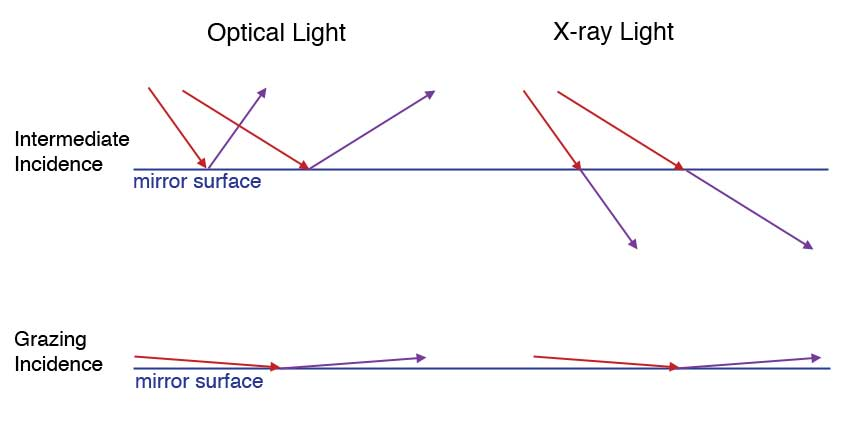
\includegraphics[width=0.7\linewidth]{Figures/grazing_incidence.jpg}
 \caption{Πάνω: πώς συμπεριφέρεται μια δέσμη οπτικού και μία δέσμη ακτίνων Χ κατά την πρόσπτωσή τους υπό μεσαία γωνία πάνω σε κάτοπτρο. Κάτω πώς συμπεριφέρονται οι ίδιες δέσμες για πρόσπτωση σχεδόν παράλληλη στην επιφάνεια- η γωνία που σχηματίζει η δέσμη με την επιφάνεια πρόσπτωσης στην περίπτωση της \textlatin{grazing incidence} για να ανακλαστεί η δέσμη ακτίνων Χ είναι στην πραγματικότητα μικρότερη από αυτήν που φαίνεται στο σχήμα. (Εικόνα από το <<\textlatin{Imagine the Universe}>> της \textlatin{NASA})}
 \label{fig:grazing_incidence}
 \end{center}
 \end{figure*}
  
\begin{figure*}
 \begin{center}
 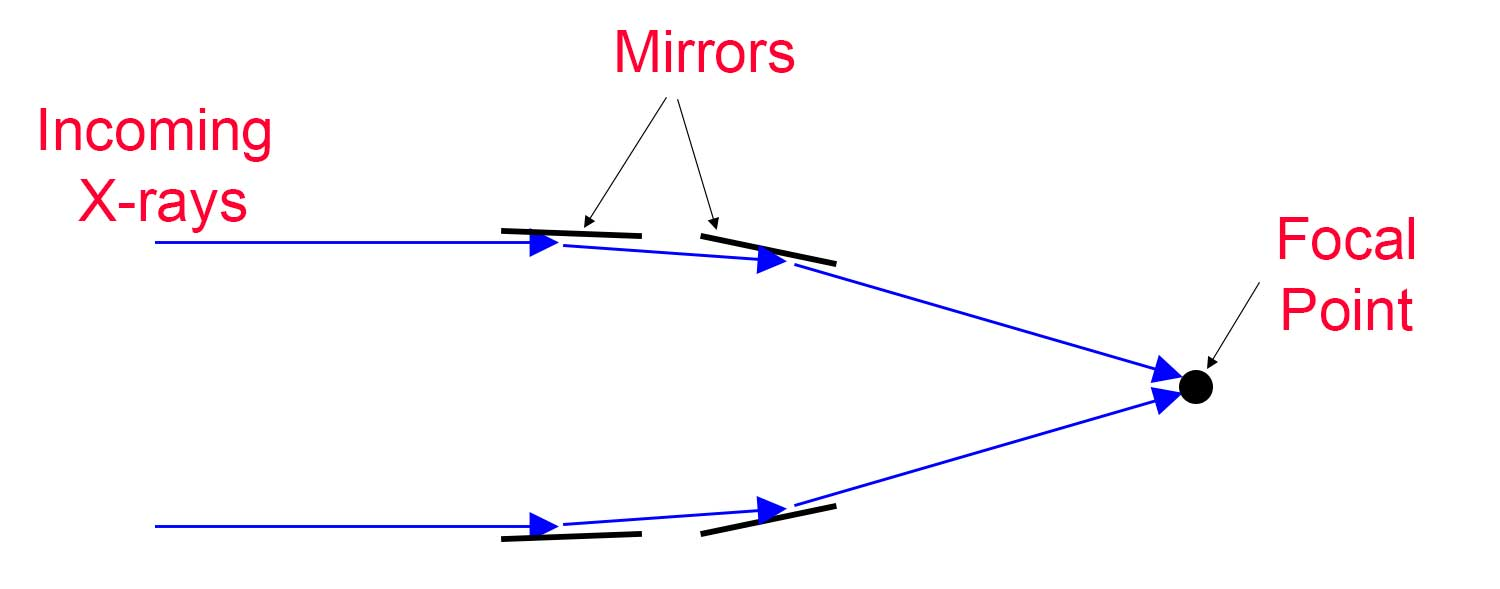
\includegraphics[width=0.7\linewidth]{Figures/xray_telescope_1mirror.jpg}
 \caption{Σχηματικό διάγραμμα κατά μήκος τομής τηλεσκοπίου ακτίνων Χ με ένα σετ κατόπτρων. Στο σχήμα με μπλε βέλη αναπαριστώνται εισερχόμενες ακτίνες Χ που προσπίπτουν σε δύο διαδοχικά κάτοπτρα (μαύρα επίπεδα) και εστιάζονται σε ένα σημείο. (Εικόνα από το <<\textlatin{Imagine the Universe}>> της \textlatin{NASA})}
 \label{fig:xray_telescope_1mirror}
 \end{center}
 \end{figure*}
 
Τα τηλεσκόπια ακτίνων Χ χρειάζονται κάτοπτρα από υλικό που ανακλά ακτίνες Χ και πρέπει να είναι προσανατολισμένα με τρόπο τέτοιον ώστε οι ακτίνες Χ να προσπίπτουν σχεδόν εφαπτομενικά με το κάτοπτρο, δηλαδή η επιφάνεια των κατόπτρων πρέπει να είναι σχεδόν παράλληλη με τις εισερχόμενες δέσμες- όπως φαίνεται στο σχήμα \ref{fig:xray_telescope_1mirror}. Για να ανακλαστεί διαδοχικά η δέσμη με γωνία σχεδόν εφαπτομενική κάθε φορά ώστε να εστιαστεί στο εστιακό επίπεδο του τηλεσκοπίου απαιτείται το τηλεσκόπιο να είναι αρκετά επίμηκες, αφού ανακατευθύνουμε τις δέσμες με γωνίες σχεδόν εφαπτομενικές στα κάτοπτρα προκειμένου να εστιαστούν.

\begin{figure*}
 \begin{center}
 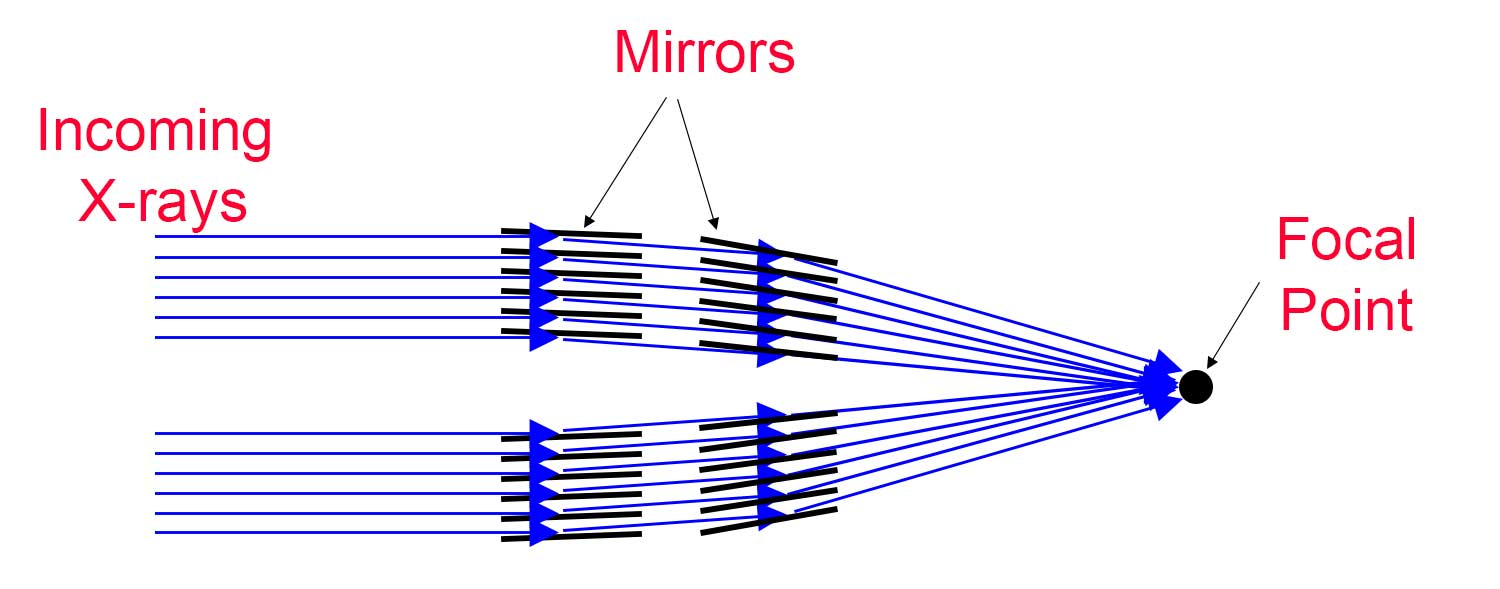
\includegraphics[width=0.7\linewidth]{Figures/xray_telescope_multimirror.jpg}
 \caption{Σχηματικό διάγραμμα κατά μήκος τομής τηλεσκοπίου ακτίνων Χ με αρκετά σετ κατόπτρων. Με ένθετα κάτοπτρα περισσότερες δέσμες εστιάζονται παρέχοντας λαμπρότερη απεικόνιση. (Εικόνα από το <<\textlatin{Imagine the Universe}>> της \textlatin{NASA})} \label{fig:multimirror}
 \end{center}
\end{figure*}

Τοποθετώντας τα κάτοπτρα στις εσωτερικές πλευρές του <<σωλήνα>> που αποτελεί τον κορμό του τηλεσκοπίου, υπάρχει ένα κενό στο κέντρο με αποτέλεσμα το τηλεσκόπιο να χάνει πολλές ακτίνες Χ. Για να λυθεί το πρόβλημα αυτό, τα τηλεσκόπια ακτίνων Χ χρησιμοποιούν κυλινδρικά κάτοπτρα και τα τοποθετούν ένθετα το ένα μέσα στο άλλο- όπως σχηματικά βλέπουμε στο σχήμα \ref{fig:multimirror}. Σημαντικό ρόλο παίζει το υλικό του κατόπτρου (υλικά με υψηλό ατομικό αριθμό Ζ ανακλούν καλύτερα υψηλοενεργειακά φωτόνια- για αυτό συχνά τα κάτοπτρα είναι επιχρυσωμένα) καθώς και η λείανση της κατοπτρικής επιφάνειας για να μην υπάρχουν σημαντικές απώλειες.

\begin{figure*}
 \begin{center}
 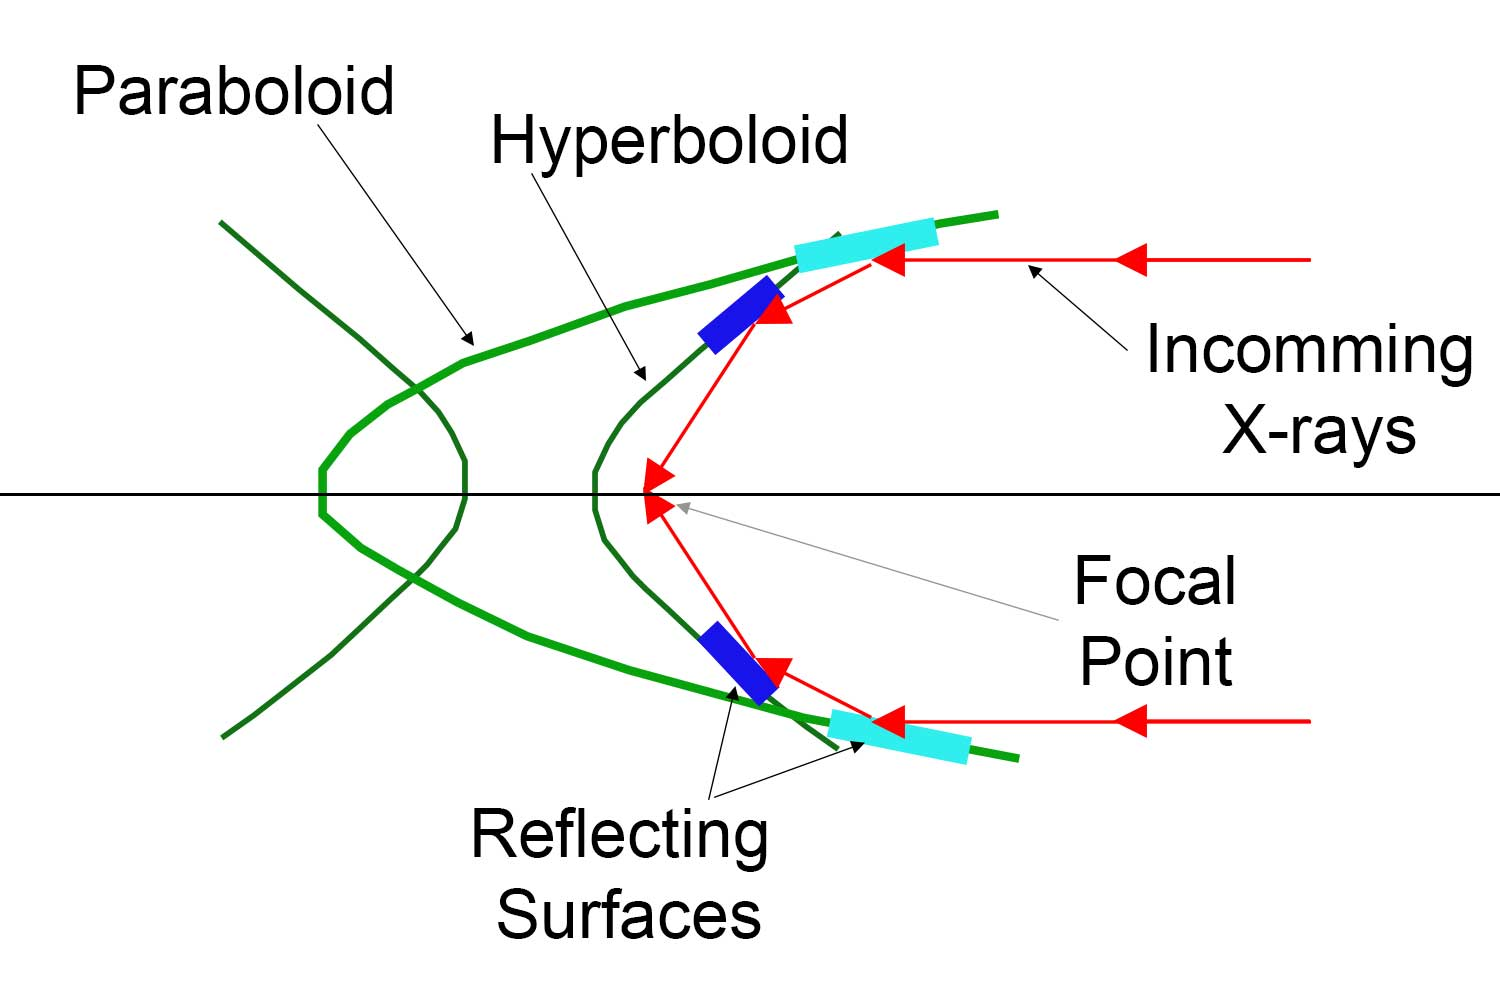
\includegraphics[width=0.7\linewidth]{Figures/wolter_typeI.jpg}
 \caption{Ο σχεδιασμός που ακολουθεί ένα τηλεσκόπιο \textlatin{Wolter} τύπου 1. Το παραβολοειδές εκ περιστροφής σχήμα των κατόπτρων και το υπερβολοειδές εκ περιστροφής σχήμα των κατόπτρων έχουν κοινό άξονα με την γραμμή παρατήρησης και κοινό εστιακό επίπεδο μεταξύ τους. (Εικόνα από το <<\textlatin{Imagine the Universe}>> της \textlatin{NASA})} \label{fig:wolter}
 \end{center}
\end{figure*} 

Η κατασκευή που χρησιμοποιείται ευρέως στην αστρονομία ακτίνων Χ και συγκεκριμένα στο τηλεσκόπιο \textlatin{XMM-Newton} λέγεται κάτοπτρο \textlatin{Wolter} τύπου 1 και είναι μια διαδοχή κατόπτρων υπερβολοειδούς σχήματος κοντά στο εστιακό επίπεδο που καταλήγουν σε παραβολοειδές σχήμα στην αντίθετη άκρη του τηλεσκοπίου- όπως φαίνεται στο σχήμα \ref{fig:wolter}. Η εικόνα σχηματίζεται στο εστιακό επίπεδο μετά από διαδοχική ολική ανάκλαση από την παραβολοειδή και την υπερβολοειδή επιφάνεια. Το σχήμα αυτό είναι μηχανικά απλό και επιτρέπει την τοποθέτηση πολλών κατόπτρων το ένα μέσα στο άλλο, αυξάνοντας έτσι την ωφέλιμη επιφάνεια ανάκλασης ώστε να έχουμε ευκρινείς παρατηρήσεις και καλές μετρήσεις για αμυδρές πηγές που δεν θα μπορούσαμε να παρατηρήσουμε διαφορετικά. 

\subsection{Το τηλεσκόπιο \textlatin{XMM-Νewton}}

Το \textlatin{XMM-Νewton} έχει τρία τηλεσκόπια ακτίνων Χ και ένα τηλεσκόπιο για οπτικό/ υπεριώδες.\\
Κάθε ένα από τα τρία τηλεσκόπια του \textlatin{XMM-Newton} αποτελείται από 58 ένθετα κάτοπτρα \textlatin{Wolter} τύπου 1 κατασκευασμένα ιδανικά για δέσμες που προσπίπτουν υπό γωνία ${0^ο} {30^\prime}$ με την επιφάνεια του κατόπτρου προσφέροντας, έτσι, υψηλή ανακλαστικότητα σε ακτίνες ενεργειών $\sim 7$ \textlatin{keV}. Το εστιακό μήκος των τηλεσκοπίων είναι $7.5$ \textlatin{m} και η διάμετρος του εξωτερικού κατόπτρου είναι $70$ \textlatin{cm}. Η διάρθρωση αυτή και το πλήθος των κατόπτρων καθιστούν το \textlatin{XMM-Newton} ένα από τα τηλεσκόπια ακτίνων Χ με την μεγαλύτερη ευαισθησία.
  
Το \textlatin{XMM-Newton} προσφέρεται για απεικόνιση ή απεικονιστική φασματοσκοπία που δεν απαιτεί διακριτική ικανότητα καλύτερη από $5$ \textlatin{arcsec} (στο σύστημα απεικόνισης του \textlatin{XMM-Newton} ένα \textlatin{pixel} αντιστοιχεί σε $4.4$ \textlatin{arcsec}) και για φασματοσκοπία υψηλής ανάλυσης για ενέργειες $0.2- 2$ \textlatin{keV} και για φασματοσκοπία εκτεταμένων αντικειμένων ($>10$ \textlatin{arcsec} και $< 1$ \textlatin{arcmin}).

\subsection{Ανιχνευτές στο \textlatin{XMM-Νewton}}
  
Το \textlatin{XMM-Νewton} έχει τα εξής όργανα καταγραφής επιστημονικών δεδομένων\cite{Handbook}: 
\begin{itemize}
    \item \textlatin{EPIC (European Photon Imaging Camera):} Τρείς κάμερες \textlatin{CCD} για απεικόνιση ακτίνων Χ, φασματισκοπία μέτριας ευκρίνειας και φωτομετρία ακτίνων Χ. Έχουμε δύο διαφορετικά είδη κάμερων \textlatin{EPIC}: \textlatin{MOS} και ΡΝ με 7 και 12 \textlatin{chip} αντίστοιχα. Το \textlatin{XMM-Νewton} φέρει δύο κάμερες \textlatin{MOS} και μία ΡΝ.
    \item \textlatin{RGS (Reflection Grating Spectrometer):}  Δύο όμοια φασματόμετρα για υψηλής ευκρίνειας φασματοσκοπική ανάλυση ακτίνων Χ και φασματο-φωτομετρία.
    \item \textlatin{ΟΜ (Optical Monitor):}  για απεικόνιση στο οπτικό/υπεριώδες και φασματοσκοπία πλεγματικού πρίσματος.
\end{itemize}

\begin{figure*}
 \begin{center}
 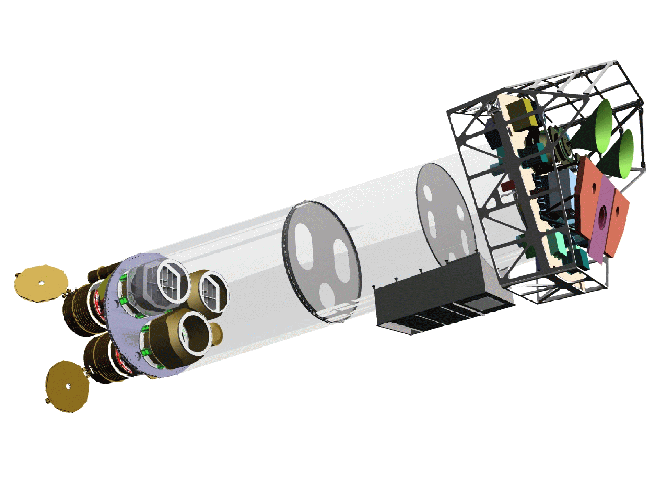
\includegraphics[width=0.9\linewidth]{Figures/img33.png}
 \caption{Σχηματικά τα μέρη που αποτελούν το παρατηρητήριο \textlatin{XMM}. Στο αριστερό άκρο, όπως φαίνεται στο σχήμα, οι τρείς μονάδες με τις συστάδες ένθετων κατόπτρων- οι δύο από τις οποίες έχουν πλεγματικά φράγματα (\textlatin{gratings}). Στο αντίθετο άκρο του παρατηρητηρίου φαίνονται τα όργανα στα εστιακά επίπεδα των τηλεσκοπίων: οι μηχανισμοί ψύξης των δύο κάμερων \textlatin{EPIC MOS} (οι δομές με μαύρο και πράσινο χρώμα), ο μηχανισμός ψύξης της \textlatin{EPIC} ΡΝ (με ανοιχτό μωβ χρώμα), οι ανιχνευτές \textlatin{RGS} (με φωτεινό γαλάζιο χρώμα) και οι μηχανισμοί ψύξης των \textlatin{RGS} (με κοκκινο-ροζ χρώμα)- δεν φαίνεται το οπτικό τηλεσκόπιο ΟΜ (βρίσκεται πίσω από την χαμηλότερη μονάδα ένθετων κατόπτρων στα αριστερά) (Εικόνα από το <<\textlatin{XMM-Newton User's Handbook, 2021.}>> \textlatin{ESA: XMM-Newton SOC})}
 \label{fig:XMMsketch}
 \end{center}
 \end{figure*}

Οι τρείς κάμερες \textlatin{EPIC} και οι δύο ανιχνευτές των φασματόμετρων \textlatin{RGS} βρίσκονται στα εστιακά επίπεδα των τηλεσκοπίων ακτίνων Χ, ενώ το ΟΜ στο τηλεσκόπιο οπτικού/υπεριώδους του παρατηρητηρίου \textlatin{XMM.} Ένα σχέδιο του παρατηρητηρίου \textlatin{XMM} φαίνεται στο σχήμα \ref{fig:XMMsketch}. Τα επιστημονικά όργανα του \textlatin{XMM} μπορούν να λειτουργούν ταυτόχρονα αλλά και αυτόνομα σε διαφορετικές καταστάσεις λειτουργίας.\\
Οι κάμερες \textlatin{EPIC} λειτουργούν ως καταμετρητές φωτονίων \textlatin{(photon counting mode)} με σταθερή συχνότητα  \textlatin{read-out} παράγοντας λίστες γεγονότων (πίνακες με μία γραμμή για κάθε καταχώρηση γεγονότος που περιλαμβάνει, μεταξύ άλλων, τα χαρακτηριστικά του γεγονότος όπως θέση, χρονική στιγμή καταγραφής και ενέργεια.)\\ 
\begin{figure*}
 \begin{center}
 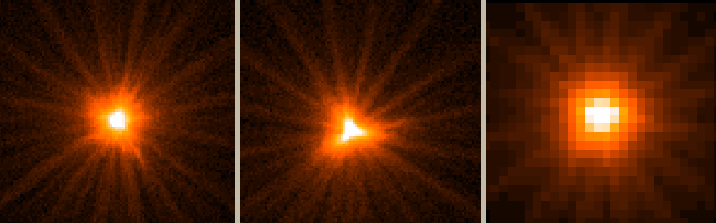
\includegraphics[width=0.9\linewidth]{Figures/PSFs.png}
 \caption{Η συνάρτηση εξάπλωσης σημείου \textlatin{PSF} για τους ανιχνευτές \textlatin{MOS1}, \textlatin{MOS2} και ΡΝ (από τα αριστερά στα δεξιά) για την ίδια πηγή στις ακτίνες Χ. Το μέγεθος \textlatin{pixel} αντιστοιχεί σε $1.1\; arcsec$ για τους ανιχνευτές \textlatin{MOS} και σε $4.1\;arcsec$ για τον ανιχνευτή ΡΝ (Εικόνα από το <<\textlatin{XMM-Newton User's Handbook, 2021.}>> \textlatin{ESA: XMM-Newton SOC})}
 \label{fig:PSFs}
 \end{center}
 \end{figure*}
\begin{figure*}%
    \centering
    \subfloat{{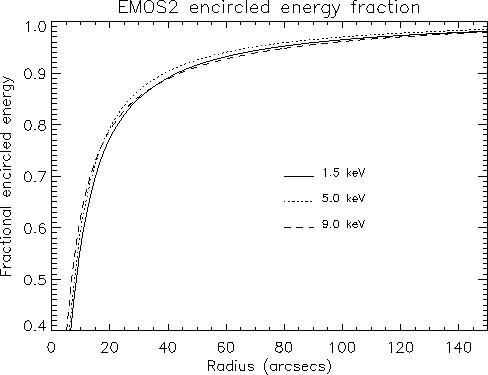
\includegraphics[width=0.46\linewidth]{Figures/EFF_M1.png} }}%
    \qquad
    \subfloat{{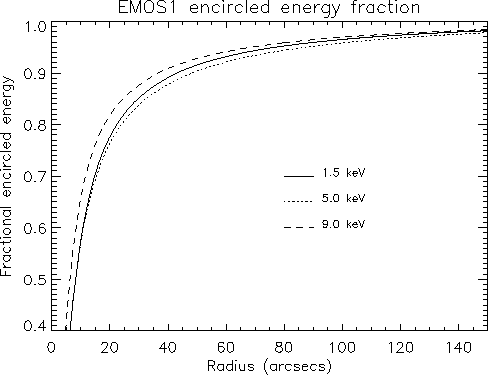
\includegraphics[width=0.46\linewidth]{Figures/EFF_M2.png} }}%
     \caption{Το κλάσμα ενεργειακής ισχύος που περικλείεται στην παρατήρηση σε συνάρτηση με την γωνιακή ακτίνα του διαφράγματος στον άξονα παρατήρησης για ακτινοβολίες διαφορετικών ενεργειών. Αριστερά: για τον ανιχνευτή \textlatin{EPIC MOS1}. Δεξιά: για τον ανιχνευτή \textlatin{EPIC MOS2}. (Εικόνα από το <<\textlatin{XMM-Newton User's Handbook, 2021.}>> \textlatin{ESA: XMM-Newton SOC})} \label{fig:EEF_MOS}
\end{figure*}
\begin{figure*}
 \begin{center}
 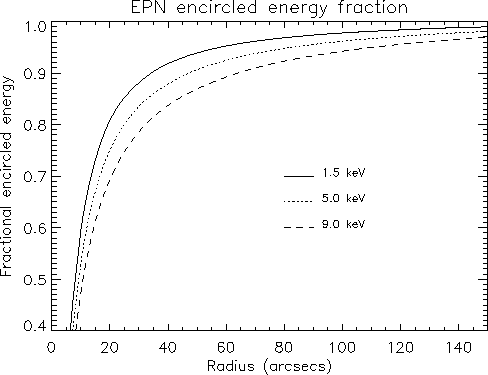
\includegraphics[width=0.7\linewidth]{Figures/EFF_PN.png}
 \caption{Το κλάσμα ενεργειακής ισχύος που περικλείεται στην παρατήρηση σε συνάρτηση με την γωνιακή ακτίνα του διαφράγματος στον άξονα παρατήρησης για ακτινοβολίες διαφορετικών ενεργειών για τον ανιχνευτή \textlatin{EPIC} ΡΝ. (Εικόνα από το <<\textlatin{XMM-Newton User's Handbook, 2021.}>> \textlatin{ESA: XMM-Newton SOC})}
 \label{fig:EEF_PN}
 \end{center}
 \end{figure*}
Η γωνιακή ικανότητα των ανιχνευτών \textlatin{EPIC} καθορίζεται από την συνάρτηση εξάπλωσης σημείου \textlatin{PSF} η οποία με την σειρά της καθορίζεται από τα κάτοπτρα (σχήμα \ref{fig:PSFs}). Οι \textlatin{EPIC MOS} και ΡΝ έχουν \textlatin{pixel} μεγέθους $40$ και $150$ m\textlatin{m} αντίστοιχα. Για το εστιακό μήκος των τηλεσκοπίαν ($7.5$ \textlatin{m}) αυτό αντιστοιχεί σε $1.1\; arcsec$ στον ουράνιο θόλο για τις \textlatin{EPIC MOS} και $4.1$ \textlatin{arcsec} για την \textlatin{EPIC PN}.\\
Ανάλογα με την γωνιακή ακτίνα του διαφράγματος, διαφορετικό ποσοστό της ροής σημειακής πηγής (δηλαδή της \textlatin{PSF}) περικλείεται στην παρατήρηση. Στα σχήματα \ref{fig:EEF_MOS} kai \ref{fig:EEF_PN} χαράσεται η συναρτησιακή αυτή σχέση για κάθε ανιχνευτή ξεχωριστά. 

Οι παρατηρήσεις των στοχευμένων \textlatin{(pointed)} πηγών έγιναν με άνοιγμα διάφραγματος ακτίνας $15$ \textlatin{arcsec} ενώ για παρατηρήσεις πηγών κατά την περιστροφή του τηλεσκοπίου \textlatin{(slew)} η ακτίνα του διάφραγματος είναι $30$ \textlatin{arcsec}\cite{RapidXMM}.
H καταγραφή του υποβάθρου γίνεται με μία μάσκα δακτυλιοειδούς σχήματος με εσωτερική ακτίνα $60$ \textlatin{arcsec} και εξωτερική ακτίνα $180$ \textlatin{arcsec}, η μάσκα αυτή επιτρέπει το άνοιγμα του διαφράγματος να περιορίζεται σε δακτύλιο μεταξύ των ακτίνων αυτών για τον υπολογισμό του υποβάθρου και προσαρμόζεται στην κλίμακα κάθε παρατήρησης πολλαπλασιάζοντας με τον λόγο των εμβαδών του διαφράγματος έκθεσης\cite{RapidXMM}. 

\subsubsection*{Απόδοση των ανιχνευτών ακτίνων Χ}

\begin{figure*}
 \begin{center}
 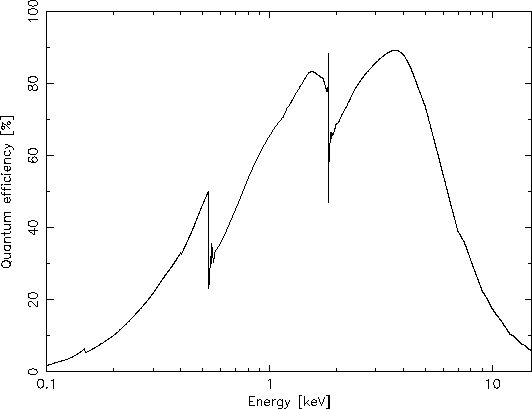
\includegraphics[width=0.7\linewidth]{Figures/mosqe.png}
 \caption{Η κβαντική απόδοση των \textlatin{chip} των ανιχνευτών \textlatin{EPIC MOS} ως συνάρτηση της ενέργειας των φωτονίων. (Εικόνα \cite{MOS})}
 \label{fig:QE_mos}
 \end{center}
 \end{figure*}
\begin{figure*}
 \begin{center}
 
\includegraphics[width=0.7\linewidth]{Figures/pnqe.png}
 \caption{Η κβαντική απόδοση των \textlatin{chip} των ανιχνευτών \textlatin{EPIC} ΡΝ ως συνάρτηση της ενέργειας των φωτονίων.(Εικόνα \cite{PN})}
 \label{fig:QE_pn}
 \end{center}
 \end{figure*}
Ένας παράγοντας που πρέπει να ληφθεί υπ>όψιν για την απόδοση των ανιχνευτών \textlatin{EPIC} είναι η κβαντική απόδοση των \textlatin{chip} των ανιχνευτών που περιορίζει τις ενέργειες που μελετάμε.
Όπως βλεπουμε στα σχήματα \ref{fig:QE_mos} kai \ref{fig:QE_pn}, τα \textlatin{chip} του ανιχνευτή ΡΝ έχουν απόδοση από $0.6-1.0$ στο ενεργειακό παράθυρο $0.15-2.0$ \textlatin{keV}, απόδοση σχεδόν 1 στο ενεργειακό παράθυρο $2.0-9.0$ \textlatin{keV} kai απόδοση $0.6-0.9$ για ενέργειες $10-15$ \textlatin{keV}, αντίθετα τα \textlatin{chip} των ανιχνευτών \textlatin{MOS} δεν έχουν συστηματικά πολύ μεγάλη απόδοση σε μεγάλο εύρος ενεργειών.

\subsection{Παρατηρήσεις του \textlatin{XMM-Νewton}}

\begin{figure*}%
    \centering
    \subfloat{{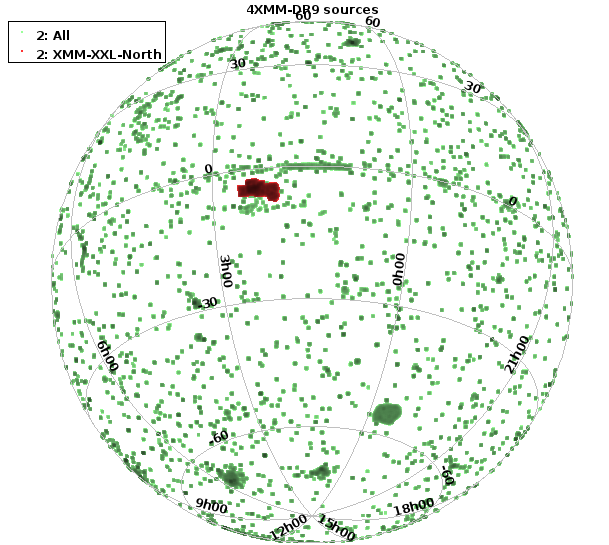
\includegraphics[width=0.46\linewidth]{Figures/4XMM-DR9 sources.png} }}%
    \qquad
    \subfloat{{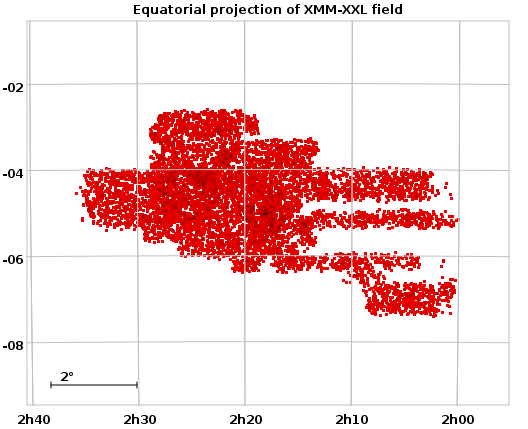
\includegraphics[width=0.46\linewidth]{Figures/EquatorialViewXMMXXL.png} }}%
     \caption{Αριστερά: Ισημερινή προβολή των πηγών που έχει καταγράψει το \textlatin{XMM-Newton} είτε στοχευμένα (\textlatin{pointed}) είτε κατά την περιστροφή του τηλεσκοπίου (\textlatin{slew}), το πεδίο \textlatin{XMM-XXL-North} απεικονίζεται με διαφορετικό χρώμα. Δεξιά: προβάλονται οι πηγές με στοχευμένες παρατηρήσεις του πεδίου \textlatin{XMM-XXL-North} σε ισημερινή προβολή. Ο οριζόντιος άξονας είναι η διορθωμένη για ιδία κίνηση ορθή αναφορά (\textlatin{RA}) και ο κατακόρυφος άξονας η διορθωμένη απόκλιση (\textlatin{Dec}). (Οι παραπάνω εικόνες παρήχθησαν χρησιμοποιώντας το πρόγραμμα απεικόνισης \textlatin{TOPCAT} \cite{TopCat} και τους καταλόγους \textlatin{4XMM-DR9}\cite{2020yCat.9059....0W} kai \textlatin{RapidXMM} \cite{RapidXMM})} \label{fig:XMMfield}
\end{figure*}
  
To \textlatin{XMM-Νewton} έχει συμμετάσχει σε πολλές έρευνες, έχει καλύψει πεδία που έχουν παρατηρηθεί ήδη από άλλα τηλεσκόπια και έχει λάβει δεδομένα τόσο με στοχευμένες (\textlatin{pointed}) παρατηρήσεις όσο και κατά την περιστροφή του (\textlatin{slew}). Ως μέρος της έρευνας \textlatin{XMM-XXL}, χαρτογραφήθηκαν από το \textlatin{XMM-Νewton} δύο νέα πεδία: το \textlatin{XMM-XXL-North} kai to \textlatin{XMM-XXL-South}, τα οποία καλύπτουν συνδυαστικά $\sim 50 $ \textlatin{deg}$^2$. Στην εικόνα \ref{fig:XMMfield} βλέπουμε μία άποψη από όλες τις παρατηρήσεις του \textlatin{XMM-Νewton} (με πράσινο χρώμα) στον ουράνιο θόλο, ενώ με κόκκινο σημειώνεται το πεδίο \textlatin{XMM-XXL-North}. Το πεδίο \textlatin{XMM-XXL-North} (με κόκκινο χρώμα στην εικόνα \ref{fig:XMMfield} αποτελεί το πεδίο στο οποίο στηρίζεται η παρούσα εργασία.
%με κοκκινο το ΧΜΜ-ΧΧΛ, που αποτελει και το βασικο πεδιο πανω στο οποιο στηριζεται η παρουσα εργασια. 
  
  
  
  
  
  
  
  
  
  
 % Fundamentals
	
	\chapter{Μεταβλητότητα των \textlatin{AGN} στις ακτίνες Χ} \label{framework}

%{\color{red}: Υπαρχουν και περιοδικες μεταβολες - Θα ελεγαν "Η εργασια αυτη επικεντρονεται στις μη περιοδικες ματαβολες στην παρατηρουμενη ροη ΑΓΝ. Οι Μεταβολες αυτες  παρατηροθβνταο σε ολα τα μηκη κυματος και θεωρειται μια απο τις ...." οχι μονο των ΑΓΝ αλλα και τον αστρικων μελανων οπων και γανικα ολων των διαδικασιων που περιλαμβανουν προσαυξηση υλης πανω σε ενα συμπαγες αντικειμωνο}


% , while optical continuum variations are thought to be related to instabilities in the more extended, colder and optically thick parts of the same disk. The simplistic assumption is that the X-ray and optical variations will be well correlated. This is true in some but not all objects. A comparison of optical and X-ray light curves in a number of sources shows that in some of these, the optical light curve “leads” the X-ray light curve, whereas in others, one finds the opposite behavior. The multiband light curves of many type-I AGNs indicate variability time scales, and variability amplitudes, that seem to be inversely correlated with source luminosity. This is clearly seen in the X-ray and optical bands, where most such studies have been conducted. There are some indications that the driver of the variability amplitude is the BH mass.\cite{netzer_2013}


%Η μεταβλητότητα στους \textlatin{AGN} τύπου Ι παρατηρείται σε όλα τα μήκη κύματος με τις γρηγορότερες μεταβολές να σημειώνονται στις υψηλότερες ενέργειες. Ματαβολές στις σκληρές ακτίνες Χ έχουνπαρατηρηθεί και σε \textlatin{AGN} τύπου ΙΙ. Η σχέση 
 
Mεταβλητότητα της ενεργειακής ροής και του φάσματος (γραμμικού ή συνεχούς) στους ενεργούς γαλαξιακούς πυρήνες παρατηρείται σε όλα τα μήκη κύματος και θεωρείται μια από τις χαρακτηριστικές ιδιότητες των \textlatin{AGN} \cite{netzer_2013}. Οι μεταβολές αυτές είναι χαρακτηριστικές και των αστρικών μελανών οπών και γενικά όλων των διαδικασιών που περιλαμβάνουν προσαύξηση ύλης σε συμπαγές αντικείμενο.\\
Στην εργασία αυτή θα επικεντρωθούμε στις μη περιοδικές μεταβολές στην παρατηρούμενη ροή \textlatin{AGN} στις μαλακές ακτίνες Χ. Αυτό σημαίνει πως οι πηγές με τις οποίες θα ασχοληθούμε είναι κατά βάση \textlatin{AGN} τύπου Ι. 

Η μεταβλητότητα στους \textlatin{AGN} τύπου Ι παρατηρείται σε όλα τα μήκη κύματος με τις γρηγορότερες μεταβολές να σημειώνονται στις υψηλότερες ενέργειες. Ματαβολές στις σκληρές ακτίνες Χ έχουν παρατηρηθεί και σε \textlatin{AGN} τύπου ΙΙ. Η σχέση του πλάτους ματαβλητότητας και της χρονικής κλίμακας της μεταβλητότητας με την συχνότητα δεν είναι ξεκάθαρη. Οι μεταβλητότητες σε διαφορετικές ενεργειακές ροές πολλές φορές συσχετίζονται και αυτό μας δίνει πληροφορίες για τις φυσικές διαδικασίες που λαμβάνουν χώρα στην κεντρική πηγή ακτινοβολίας. Για παράδειγμα μεταβλητότητα στις ακτίνες Χ έχει παρατηρηθεί να συσχετίζεται με μεταβλητότητα της ίδιας πηγής στο οπτικό \cite{2006ASPC..360..101U} \cite{2006ASPC..360..111G}, ενώ μεταβλητότητα στις ακτίνες Χ έχει παρατηρηθεί να συσχετίζεται με μεταβλητότητα στο υπεριώδες \cite{2005A&A...430..435A}. Οι μεταβολές στις ακτίνες Χ ενδεχομένως οφείλονται σε αστάθειες του στέμματος ή του δίσκου προσαύξησης, ενώ οι μεταβολές στο οπτικό ενδεχομένως οφείλονται σε εκτενή, ψυχρότερα και οπτικά πυκνά τμήματα του δίσκου. Ο συσχετισμός των μεταβολών σε διαφορετικά μήκη κύματος δείχνει πιθανή απορρόφηση και επανεκπομπή του αρχικού σήματος από ύλικό της δομής του ενεργού γαλαξιακού πυρήνα.
%({\color{red}: Γιατι? Τι δειχνει αυτο? πχ παρομοιοι φυσικοι μιχανισμοι κλπ), επιπλεον πιαθνον το ενα μηκος κμματος (οπτικο) να ακολουθει τις ακτινες-Χ οποτε βελπει κανεις την ανταποκριση της υλης στο αρχικο σημα....}.  \\

Πιθανές αιτίες της παρατηρούμενης μεταβλητότητας των \textlatin{AGN} είναι μεταβολές στην διάχυση ενέργειας, μη-αξισυμμετρικές δομές, μετάπτωση κεκλιμένων ροών \cite{Brandt}, ή αλλαγές στον ρυθμό προσαύξησης, εκλάμψεις στον δίσκο προσαύξησης, κίνηση θερμών κηλίδων γύρω από την κεντρική \textlatin{SMBH} και (για μεγάλες χρονικές κλίμακες) κίνηση νεφών υδρογόνου που αποκρύπτουν την κεντρική πηγή \cite{2004astro.ph..9151H}.

%({\color{red}: Δεν εχεις εξηγησει τι ειναι \textlatin{PSD}. Επιπλεον γιατι εχωριστο κεφαλαιο για τις ακτινες-Χ. Ισως απλα να εξηγησεις οτι οι ακτινες-Χ παραγονται σε περιοχες πολυ κοντα απο τη μαυρη τρυπα και συνεπως παραεχουν πληροφοειες για την φυσικη της προσασυξησης υλης. για τις διαστασεις της περιχοης εκπμπης. Επιπλεον οι ακτινες-Χ εχουν το καλο οτι αστρικες διαδικασιες παραγουν σχεδον καθολου ακτινοβολια στις ακτινες-Χ. Σε αντιθεση στο οπτικο/υπερυθρο ο γαλαξιας εχειο σημαντικη συνεισφορα η ακομα και υπερεχει (δες πχ https://ui.adsabs.harvard.edu/abs/2015A\%26ARv..23....1B/abstract) και συνεπως μελεταει κανεισ την μετβαλητηοτα λογω της διαδικασοαιας προσαυξησης  και δεν}).

\section{Φασματική πυκνότητα ενεργειακής ισχύος(\textlatin{PSD})}

%{\color{red}: not only at X-rays at any wavelength Για τη μελετη της μεταβλητοτας απαιτουνται παρατηρησεις σε....}
Για την μελέτη μεταβλητότητας αστρονομικών πηγών σε οποιαδήποτε μήκη κύματος χρησιμοποιούμε καμπύλες φωτός (αλλιώς χρονοσειρές), δηλαδή πεπερασμένες σειρές $x(t_i)$ από μετρήσεις ροών $x_i$ με $Ν$ το πλήθος διακριτά σημεία που μετρήθηκαν σε χρόνους $t_i$ me $i=1,2,...,N$. Στα όργανα μέτρησης ακτίνων Χ έχουμε καταγραφές φωτονίων σε διακριτά χρονικά διαστήματα $(t_i , t_{i+1})$\cite{Grant2019}.\\
Η \textlatin{PSD} είναι ένας τρόπος να απεικονίσουμε την μεταβλητότητα της ισχύος ενός σήματος συναρτήσει της χρονικής συχνότητας \textlatin{Fourier} και εκτιμάται υπολογίζοντας το περιοδόγραμμα \cite{Vaughan2}.
Το περιοδόγραμμα είναι μία διακριτή συνάρτηση ισχύος συναρτήσει χρονικής συχνότητας $ P (f_j)$ η οποία εκτιμά την συνεχή \textlatin{PSD} $\mathcal{P}(f)$ (η οποία στις χρονοσειρές \textlatin{AGN} σε μια πρώτη προσέγγιση συμπεριφέρεται ως $ \mathcal{P}(f) \propto f^{-\alpha}$, με το $\alpha \approx 2$ κατά μέσο όρο). Αν τα δεδομένα (η καμπύλη φωτός $x(t_i)$) ακολουθούν ομοιόμορφη δειγματοληψία (με περίοδο συλλογής $\Delta T$), το περιοδόγραμμα είναι ο διακριτός μετασχηματισμός \textlatin{Fourier} της καμπύλης φωτός $X(f_j)$, κανονικοποιημένος κατά $\sqrt{\frac{\Delta T}{N}}$ ώστε τα πλάτη να είναι ανεξάρτητα της συχνότητας δειγματοληψίας και του μήκους της καμπύλης φωτός. Το αποτέλεσμα του κανονικοποιημένου αυτού μετασχηματισμού είναι μιγαδική διακριτή συνάρτηση $X(f_j)$ με $Ν/2$ ισαπέχουσες συχνότητες η οποία, αφού τετραγωνιστεί με την μιγαδική συζυγή της, με κατάλληλη κανονικοποίηση αποτελεί το περιοδόγραμμα\cite{Vaughan2}:
\begin{equation} P(f_j) = \frac{2}{\overline{x}^2} |X(f_j)|^2  \end{equation}

\subsection{Θόρυβος \textlatin{Poisson}}
Αν οι χρονοσειρές είναι σήμα καταμέτρησης φωτονίων (και όχι ροές), όπως συμβαίνει στην αστρονομία ακτίνων Χ, και ομαδοποιηθούν σε χρονικά διαστήματα $\Delta T$, τότε η επίδραση θορύβου \textlatin{Poisson} έχει ώς αποτέλεσμα την πρόσθεση μιας σχεδόν σταθερής ποσότητας ισχύος στο περιοδόγραμμα σε όλες τις συχνότητες \cite{2003MNRAS.345.1271V} όπως βλέπουμε και στο σχήμα \ref{fig:LCandPSD}.

\begin{figure*}%
    \centering
    \subfloat{{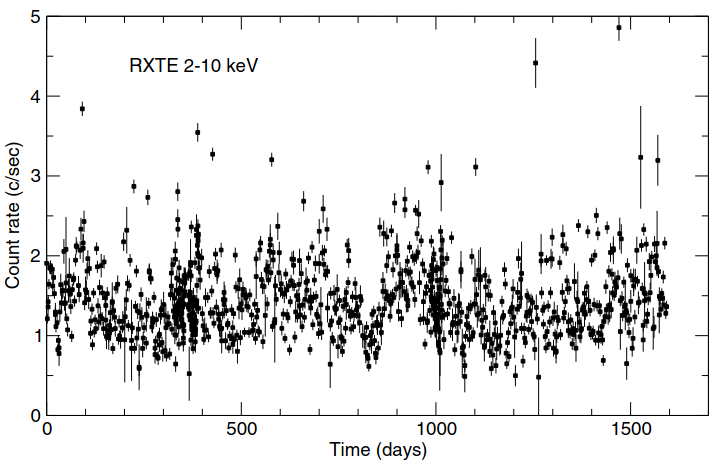
\includegraphics[width=0.42\linewidth]{Figures/PapadakisLC.png} }}%
    \qquad
    \subfloat{{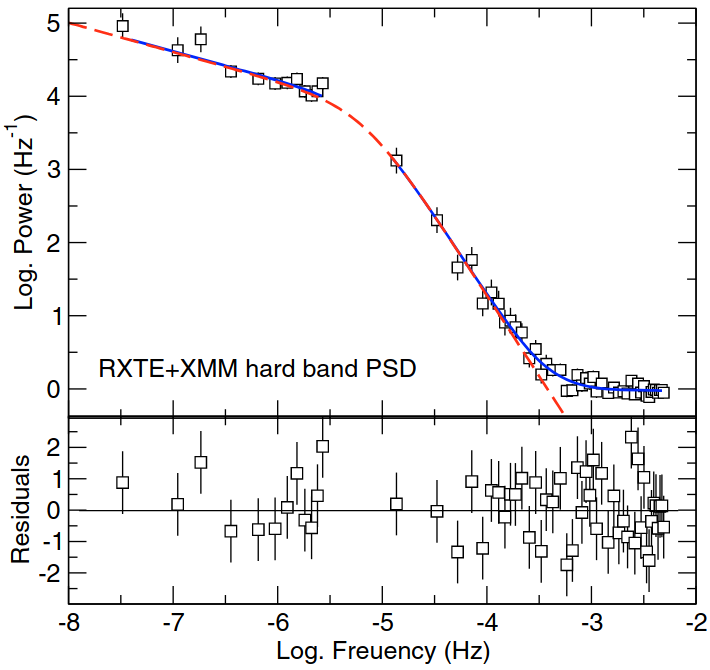
\includegraphics[width=0.5\linewidth]{Figures/PapadakisPSD.png} }}%
     \caption{Αριστερά: Δείγμα καμπύλης φωτός ακτίνων Χ ενεργού γαλαξιακού πυρήνα. Δεξιά: Ο διακριτός μετασχηματισμός \textlatin{Fourier} της καμπύλης φωτός- κατάλληλα κανονικοποιημένος- μας δείνει το περιοδόγραμμα (διακριτά σημεία) το οποίο προσεγγίζει την \textlatin{PSD} (κόκκινη διακεκομένη γραμμή) ενώ παρατηρούμε και το σταθερό υπόβαθρο θορύβου \textlatin{Poisson} (φαίνεται καθαρά στην μπλέ συνεχή καμπύλη ως σταθερά στις μεγάλες συχνότητες)\cite{2010A&A...518A..28P}.} \label{fig:LCandPSD}
\end{figure*}

\subsection{Μέσος όρος και ομαλοποίηση περιοδογράμματος}

Το περιοδόγραμμα σε μια δεδομένη συχνότητα $P(f_0)$ διασπείρεται γύρω από την \textlatin{PSD} $\mathcal{P}(f_0)$ ακολουθώντας μια κατανομή $\chi^2$ δύο βαθμών ελευθερίας:
\begin{equation}
    P(f_0) = \mathcal{P}(f_0)\dfrac{\chi^2_2}{2}
\end{equation}
και είναι ασύμφωνο με την \textlatin{PSD}, καθώς η διασπορά στο περιοδόγραμμα δεν μειώνεται αυξάνοντας το πλήθος των σημείων στην καμπύλη φωτός. Προκειμένου να περιοριστεί η διασπορά παίρνουμε τον μέσο όρο του περιοδογράμματος (είτε ομαδοποιώντας (\textlatin{bin}) τις συχνότητες είτε παίρνοντας μέσο όρο τμημάτων δεδομένων) με αποτέλεσμα ο μέσος όρος αυτός του περιοδογράμματος να συμφωνεί με την \textlatin{PSD}\cite{2003MNRAS.345.1271V}.
Για να περιοριστεί η διασπορά το περιοδόραμα υποβάλεται και σε <<vομαλοποίηση>> (\textlatin{smoothing}), δηλαδή υπολογίζεται η ενεργειακή πυκνότητα σε μία συχνότητα ως μέσος όρος με ειδικό βάρος (\textlatin{weighted average}) των γειτονικών τιμών του περιοδογράμματος. Η συνάρτηση ειδικού βάρους $W$ λέγεται <<φασματικό παράθυρο>> \cite{1993MNRAS.261..612P}.

\subsection{Γενική μορφή \textlatin{PSD} ενεργών γαλαξιών}
Για κοντινά \textlatin{AGN} η προσαρμογή (\textlatin{fitting}) φασματικών δεδομένων  έχει ως αποτέλεσμα την μοντελοποίηση των \textlatin{PSD} ενεργών γαλαξιών είτε ώς νόμο δύναμης ($\mathcal{P}(f)\propto f^{-\alpha}$), είτε ώς κυρτωμένο νόμο δύναμης με συχνότητα ανακοπής $f_b$\cite{2017MNRAS.471.4398P}.
 
\section{Ολοκλήρωμα της ενεργειακής ισχύος}

Το αναλυτικό ολοκλήρωμα της (συνεχούς) συνάρτησης της \textlatin{PSD} $\mathcal{P}(f)$ μεταξύ δύο συχνοτήτων ($f_1$ και $f_2$) είναι ένα μέτρο της μέσης φασματικής ισχύος του σήματος και μας δίνει την συνεισφορά των διακυμάνσεων μεταξύ των αντίστοιχων κλιμάκων χρόνου ($1/f_1$ και $1/f_2$) στην αναμενόμενη τιμή της (<<πραγματικής>>) διακύμανσης\cite{2003MNRAS.345.1271V}:
\begin{equation} <\mathcal{S}^2> = \int_{f_1}^{f_2} \mathcal{P}(f)df  \label{eq:integratedPSD} \end{equation}
Αντίστοιχα, για διακριτή χρονοσειρά, το <<vολοκληρωμένο>> περιοδόγραμμα μας δίνει την παρατηρούμενη διακύμανση για την συλλογή δεδομένων\cite{2003MNRAS.345.1271V}: 
\begin{equation} S^2 = \sum_{j=1}^{N/2} P(f_j)\Delta f \label{eq:integratedperiodogram} \end{equation}
Όπου $\Delta f$ είναι η διακριτότητα στις συχνότητες του διακριτού μετασχηματισμού \textlatin{Fourier} ($\Delta f = \frac{1}{N\cdot \Delta T}$). \\
Η συνολίκή διακύμανση μιας πραγματικής καμπύλης φωτός είναι το ολοκλήρωμα του περιοδογράμματος $P(f_j)$ από την χαμηλότερη συχνότητα του διακριτού μετασχηματισμού \textlatin{Fourier} έως την υψηλότερη \cite{2003MNRAS.345.1271V}. Ο διακριτός μετασχηματισμός \textlatin{Fourier} υπολογίζεται σε $Ν/2$ το πλήθος ισοκατανεμημένες συχνότητες $f_j = \frac{j}{N\cdot \Delta T}$ me $(j = 1, 2, . . . , N/2)$, έτσι η χαμηλότερη συχνότητα του μετασχηματισμού είναι $f_1 = \frac{1}{N \cdot \Delta T}$ και η υψηλότερη $f_{Nyq} = \frac{1}{2  \Delta T}$ \cite{Vaughan2}.\\
H διακύμανση για την καμπύλη φωτός (χρονοσειρά) που συλλέγουμε για μια πηγή είναι (υπολογισμένη απόστοιχεία φωτομετρίας της καμπύλης φωτός): 
\begin{equation} S^2 = \frac{1}{N-1} \sum_{i=1}^{N} (x_i-\overline{x})^2 \label{eq:fluxvariance}\end{equation}
Όπου $\overline{x}$ είναι ο αριθμητικός μέσος των $x_i$ σημείων της χρονοσειράς ροής (καμπύλης φωτός). Αυτή διαφέρει από μια συλλογή δεδομένων (παρατήρηση) σε άλλη συλλογή δεδομένων της ίδιας πηγής, αφού το περιοδόγραμμα είναι μια αναπαράσταση της πραγματικής \textlatin{PSD} που εξαρτάται από την υλοποίηση της συλλογής δεδομένων (χρονοσειρά).\\
Στο όριο μεγάλου $Ν$ αυτές οι δύο προσεγγίσεις διακύμανσης (ολοκλήρωμα περιοδογράμματος \ref{eq:integratedperiodogram} και διακύμανση ροής \ref{eq:fluxvariance}) είναι ταυτοτικές. Η κανονικοποιημένη διακύμανση είναι $\frac{S^2}{\overline{x}^2}$ \cite{2003MNRAS.345.1271V}.

%%===================================%
%%===================================%
%%===================================%
\section{H \textlatin{NXSV} ως μέγεθος εκτίμησης μεταβλητότητας}

\subsection{Κανονικοποιημένη πλεονάζουσα διακύμανση(\textlatin{NXSV}) $\sigma_{rms}^2$}
 
Η ανάλυση των \textlatin{PSD} (μέσω περιοδογράμματος) είναι ένα εξαιρετικό εργαλείο για να εξεταστούν και να χαρακτηριστούν οι ιδιότητες της μεταβλητότητας των \textlatin{AGN}, ωστόσο, για να αποδόσει πλήρως απαιτεί μακροσκελείς αδιάκοπες παρατηρήσεις με διεξαγωγή παρακολουθήσεων ειδικών προδιαγραφών. Τέτοιου είδους παρατηρήσεις δεν διατίθενται για μεγάλο αριθμό πηγών, όμως υπάρχουν βραχείες παρατηρήσεις στις ακτίνες Χ με αρκετά μεγάλο λόγο σήματος προς θόρυβο (\textlatin{S/N}) πληθώρας \textlatin{AGN}- ιδίως για το παρατηρητήριο \textlatin{XMM-Newton}, λόγω της μεγάλης ευαισθησίας του και του εύρους των ενεργειών που καλύπτει. \\
Ένα χρήσιμο και πρακτικό εργαλείο για την ανάλυση ελλειπών δεδομένων είναι η πλεονάζουσα κανονικοποιημένη διακύμανση(\textlatin{NXSV}) $\sigma_{rms}$:
\begin{equation} \sigma^2_{rms} = \frac{1}{N \cdot {\overline{x}}^2 }   \sum_{i=1}^{N}  [ (x_i -\overline x)^2  - x_{err, i}^2]  \label{eq:NXSVformula}\end{equation}
Όπου $\overline x$ η μέση ροή στην χρονοσειρά $x_i$ ροών με $Ν$ το πλήθος σημεία, ενώ $x_{err, i}$ είναι η αβεβαιότητα στην μέτρηση ροής $x_i$. \\
Ο όρος $ \frac{1}{N }   \sum_{i=1}^{N}   (x_i -\overline x)^2  $ αναπαριστά την διακύμανση του σήματος, ο όρος $ \frac{1}{N }   \sum_{i=1}^{N}  x_{err, i}^2 $ αναπαριστά την διακύμανση του στατιστικού σφάλματος (θορύβου), η διαφορά των δύο είναι η πλεονάζουσα διακύμανση, και κανονικοποιώντας με τον παράγοντα $ \frac{1}{{\overline{x}}^2 }$ προκύπτει η κανονικοποιημένη πλεονάζουσα διακύμανση.\\
Η \textlatin{NXSV} είναι η μέση τετραγωνική απόκλιση που μετράμε στην καμπύλη φωτός διορθωμένη κατά το στατιστικό σφάλμα και είναι ένα μέγεθος που ποσοτικοποιεί την διακύμανση, αποτελεί δηλαδή ένα <<πλάτος>> μεταβλητότητας\cite{2004ApJ...611...93P}.\\
Σε αντιπαραβολή με την ολοκλήρωση περιοδογράμματος (\ref{eq:integratedperiodogram} ) που προσεγγίζει το ολοκλήρωμα της \textlatin{PSD} (\ref{eq:integratedPSD}), η \textlatin{NXSV} είναι το ολοκλήρωμα της \textlatin{PSD} από μία ελάχιστη κλίμακα χρόνου (μέγιστη συχνότητα) μέχρι μία μέγιστη κλίμακα χρόνου (ελάχιστη συχνότητα), η μεταβολή στην ροή επιφέρει μεταβολή στο σχήμα της \textlatin{PSD} ή στην συχνότητα αποκοπής (για κυρτωμένη \textlatin{PSD}), έτσι, αφού το φάσμα αλλάζει, με την ολοκλήρωση καταγράφουμε το πλάτος της μεταβλητότητας.\\  
Η \textlatin{NXSV} δεν προσφέρει τόση πληροφορία όσο η φασματική ανάλυση των \textlatin{PSD}, αλλά μπορεί να χρησιμοποιηθεί για να ελέγξει ή να επιβεβεώσει αποτελέσματα από φασματική ανάλυση μεμονωμένων \textlatin{AGN} σε μεγάλους πληθυσμούς καθώς και για να ελέγξει τον συσχετισμό ύπαρξης μεταβλητότητας και πλάτους μεταβλητότητας με άλλες φυσικές παραμέτρους των \textlatin{AGN}\cite{2012A&A...542A..83P}.

%%===================================%

\subsection{Αβεβαιότητα και μεροληψία στην \textlatin{NXSV}}

\subsubsection*{Αβεβαιότητα}
Η \textlatin{NXSV}, όπως ορίστηκε στην εξίσωση \ref{eq:NXSVformula}, εκτιμά την εγγενή μεταβλητότητα της καμπύλης φωτός κατά μέγιστη πιθανότητα \textlatin{(maximum likelihood- ML)} μόνο στην περίπτωση που έχουμε όμοια, κανονικά κατανεμημένα σφάλματα στις μετρήσεις της χρονοσειράς. Αν αυτό δεν συμβαίνει, τότε δεν υπάρχει αναλυτικός τρόπος μέγιστης πιθανότητας \textlatin{(ML)} που να εκτιμά την εγγενή μεταβλητότητα και απαιτείται αριθμητική προσέγιση\cite{2017MNRAS.471.4398P}. Ωστόσο, πρακτικά, οι δύο αυτοί τρόποι (αναλυτική $\sigma_{rms}^2$ για ίδια κανονικά σφάλαματα και αριθμητική $\sigma_{ML}^2$ για ανομοιόμορφα σφάλματα) για ρεαλιστικές καμπύλες φωτός με <<vαραιές>> καταγραφές δεδομένων δίνουν όμοια αποτελέσματα\cite{2013ApJ...771....9A}. Αυτό είναι αναμενόμενο, καθώς η αβεβαιότητα που οφείλεται σε στοχαστικό θόρυβο \textlatin{(red noise)} στην καμπύλη φωτός είναι πολύ μεγαλύτερη της αβεβαιότητας που οφείλεται στην προσέγγιση αναλυτικής λύσης $\sigma_{rms}^2$.\\

%The datasets considered thus far have been ideal, in the sense that they are free from flux uncertainties. In real life, however, a lightcurve xi will have finite uncertainties σerr,i due to measurement errors (such as Poisson noise in the case of an X-ray photon counting signal). These uncertainties on the individual flux measurements will contribute an additional variance. This leads to the use of the ‘excess variance’ (Nandra et al. 1997; Edelson et al. 2002) as an estimator of the intrinsic source variance. This is the variance after subtracting the contribution expected from measurement errors. --------------------\\ The normalised excess variance is given by σNXS2= σXS2/x̄ 2 and the fractional root mean square (rms) variability amplitude (Fvar ; Edelson, Pike & Krolik 1990; Rodriguez-Pascual et al. 1997) is thesquare root of this, i.e. \cite{2003MNRAS.345.1271V} 

% An empirical estimate of the mean and standard deviation of the variance can be made given M non-overlapping data segments The advantage of the above method is that it requires no assumption about the shape of the PSD, The drawback is that it requires asubstantial amount of data to produce a single, robust variance estimate. An alternative approach is to estimate the standard deviationof the variances Si based on simulations. Given an assumed shape for the PSD it is possible to calculate the distribution of variances expected for a stationary process..  the distribution depends on the slope of the PSD. The distribution becomes more normal at flatter slopes and more asymmetric at steep slopes. \cite{2003MNRAS.345.1271V}  

%the uncertainty in the variance estimate caused by Poisson noise.  the error on σNXS2 decreases as the S/N in the light curve is increased according to: ----- this only accounts for the effect of flux measurement errors (such as Poisson noise) in a given light curve \cite{2003MNRAS.345.1271V} 


%The bias certainly depends on the PSD slope. For the continuous sampling case, b is always smaller than 1, and decreases with increasing β. This is due to the fact that the variance measured on any given timescale range will be affected by leakage effects that, in the case of red-noise PSDs, tends to add power coming from nearby, lower frequencies to the observed lightcurve segment. This ”leakage effect” becomes ”stronger” with increasing β \cite{2013ApJ...771....9A}
\subsubsection*{Μεροληψία}
Σύμφωνα με μελέτες\cite{2013ApJ...771....9A}, η μεροληψία (\textlatin{bias}) στην εκτίμηση της \textlatin{NXSV} ώς ολοκλήρωμα της αναλυτικής συνάρτησης \textlatin{PSD} (εξίσωση \ref{eq:integratedPSD}) είναι σημαντική όταν η ελάχιστη συχνότητα ολοκλήρωσης (που συνδέεται με την μέγιστη χρονική κλίμακα $f_{min} =1/Τ_{max}$) είναι μεγαλύτερη της συχνότητας αποκοπής $f_b$ των \textlatin{PSD} των μοντέλων. Αυτό συμβαίνει διότι η μεροληψία οφείλεται σε φαινόμενα \textlatin{aliasing} που οφείλονται σε <<διαρροή>> ισχύος από χαμηλότερες συχνότητες, οπότε η μεροληψία εξαρτάται από την λογαριθμική κλίση της \textlatin{PSD}.\\
Σε περίπτωση που έχουμε μεροληψία, η διόρθωση της μεροληπτικής $\sigma_{rms}^2$ είναι ένας πολλαπλασιαστικός παράγοντας $ 0.48^{\alpha-1}$ για \textlatin{PSD} που συμπεριφέρονται τοπικά σαν νόμος δύναμης φασματικού δείκτη $\alpha $\cite{2013ApJ...771....9A}:
\begin{equation}
    \sigma_{rms}^2\mbox{\textlatin{(bias corrected)}} = \sigma_{rms}^2 \times (0.48)^{\alpha-1}
\end{equation}
Για καμπύλες φωτός που αποτελούνται από δεδομένα που συλλέχθηκαν με άτακτο τρόπο, θα υπάρχουν χρονικές κλίμακες για τις οποίες δεν θα έχουμε επαρκή τακτικά συλλεγμένα δεδομένα. Στην περίπτωση αυτή η \textlatin{NXSV} εκτιμά μόνο την συνεισφορά των χρονικών κλιμάκων με <<καλά>> δεδομένα στην μεταβλητότητα της πηγής\cite{2013ApJ...771....9A}. 

%%===================================%
%%===================================%
%%===================================%

\section{\textlatin{Ensemble NXSV}}

Οι παρατηρήσεις ενός μεμονομένου \textlatin{AGN} με τηλεσκόπια ακτίνων Χ είναι συχνά λιγοστές και διάσπαρτες, αυτό καθιστά δύσκολη την μελέτη μίας πηγής. \\
Θεωρούμε ότι η απεριοδική μεταβλητότητα των \textlatin{AGN} είναι στοχαστική διαδικασία, έτσι κάθε καμπύλη φωτός μπορεί να ερμηνευθεί ως η υλοποίηση υποκείμενων στατιστικών ιδιοτήτων. Ακριβώς για αυτόν τον λόγο, αν έχουμε πολλαπλές καμπύλες φωτός για μία πηγή δεν μας δίνει η κάθε μία την ίδια μέτρηση μεταβλητότητας με κάθε άλλη - τότε θα βγάζαμε σωστότερα συμπεράσματα αν παίρναμε τον μέσο όρο των καμπύλων φωτός της πηγής αυτής. Στις μακρόχρονες έρευνες \textlatin{AGN} δεν έχουμε πολλαπλές καμπύλες φωτός, και συχνά η καμπύλη φωτός που έχουμε έχει διάσπαρτα δεδομένα.\\ 
Κάνοντας την παραδοχή ότι μια συλλογή \textlatin{AGN} ειναι σχετικά ομοιόμορφη, δηλαδή αποτελείται από πηγές με ίδιες ιδιότητες (αυτό μπορεί να γίνει με κριτήριο την λαμπρότητα της πηγής ή την ερυθρομετατόπιση ή άλλα χαρακτηριστικά), τότε μπορούμε να υπολογίσουμε την \textlatin{ensemble NXSV}, δηλαδή την \textlatin{NXSV} μιας συλλογής αντικειμένων. Αυτό γίνεται παίρνοντας τον μέσο όρο των καμπυλών φωτός που αντιστοιχούν στην ομάδα ομοίων \textlatin{AGN} και χειριζόμαστε την μέση αυτή καμπύλη φωτός σαν να προέρχεται από μία πηγή της οποίας τα χαρακτηριστικά αντιπροσωπεύουν στατιστικά το δείγμα. Έτσι έχουμε πολύ περισσότερα δεδομένα και τα συμπεράσματα που προκύπτουν θεωρούμε ότι αντιπροσωπεύουν όλους τους \textlatin{AGN} του πληθυσμού, έχουν δηλαδή όμοιες στατιστικές ιδιότητες\cite{2013ApJ...771....9A}. 

%We show below that, in order to derive a more robust estimate of the intrinsic source variance, we need to collect repeated observations of the same source or to use large samples of sources (assuming they have the same variability properties) in order to compute ”ensemble” estimates, which have more favourable statistical properties. \cite{2013ApJ...771....9A}
Όταν μετράμε \textlatin{ensemble NXSV}, φτιάχνουμε ομάδες \textlatin{(bin)} από πηγές \textlatin{(AGN)} για κάθε μια από τις οποίες έχουμε υπολογίσει \textlatin{NXSV} σύμφωνα με τον τύπο \ref{eq:NXSVformula} για $N$ το πλήθος παρατηρήσεων (σημείων καμπύλης φωτός) που διαθέτουμε για κάθε πηγή. Οι ομάδες αυτές αποτελούνται από $n$ το πλήθος \textlatin{(AGN)}, όπου διαλέγουμε $n = 5, 10, 20, 50$ ή όποια ομαδοποίηση είναι κατάλληλη. Για κάθε τέτοια ομάδα \textlatin{(AGN)}  υπολογίζουμε την μέση \textlatin{ensemble NXSV}:
\begin{equation} \overline{\sigma^2_{rms}} = \frac{1}{n} \sum_{i=1}^n \sigma^2_{rms, i} \label{eq:EnsembleNXSV} \end{equation}
Όπου $\sigma^2_{rms, i}$ η \textlatin{NXSV} κάθε πηγής για τις $n$ το πλήθος πηγές. Η αβεβαιότητα στην \textlatin{ensemble NXSV} είναι αβεβαιότητα μέσης τιμής\cite{2013ApJ...771....9A}: 
\begin{equation} \overline{\sigma^2_{rms}}_{err} =\sqrt{  \dfrac{\sum_{i=1}^n \big(\sigma^2_{rms, i} - \overline{\sigma^2_{rms}} \big)^2  }{n(n-1)} } \label{eq:EnsembleNXSVerr} \end{equation}
 %The mean of these distributions is identical to the mean of the σNXV,sparse 2 distribution in the case when β = 1.5, but their standard deviation is significantly smaller than the standard deviation of σNXV,sparse 2 and the distributions are more symmetric. In fact, a Kolmogorov-Smirnov test performed on the 5, 10, 20 and 50-points mean-σ NXV2 distributions indicates that only for the 5-points grouping we can reject the hypothesis of Gaussian distribution at > 95\% level. \cite{2013ApJ...771....9A}
Η χρήση της \textlatin{ensemble NXSV} προτείνεται ανεπιφύλακτα \cite{2013ApJ...771....9A} όταν έχουμε πολλές καμπύλες φωτός για την ίδια πηγή ή όταν έχουμε καμπύλες φωτός πολλών πηγών με ίδιες ιδιότητες. Σύμφωνα με μελέτες που έγιναν χρησιμοποιώντας προσομοιώσεις\cite{2013ApJ...771....9A}, για $n \geq 20$ πλήθος καμπύλων φωτός η κατανομή της μέσης \textlatin{NXSV} (όπως ορίζεται από την σχέση \ref{eq:EnsembleNXSV}) θα είναι αρκετά συμμετρική και προσεγγίζεται από κατανομή \textlatin{Gauss}, ενώ η τυπική απόκλισή της θα προσεγγίζεται από το σφάλμα μέσης τιμής (όπως ορίζεται από την σχέση \ref{eq:EnsembleNXSVerr}). Το αποτέλεσμα αυτό ισχύει για όλες τις κλίσεις στην \textlatin{(PSD)}, ανεξάρτητα από το μοτίβο συλλογής \textlatin{(sampling pattern)} της χρονοσειράς- δηλαδή αν η καμπύλη φωτός έχει πυκνά ή αραιά σημεία- αρκεί οι μεμονομένες καμπύλες φωτός να μην έχουν πολύ θόρυβο, δηλαδή να έχουν μεγάλο λόγο σήματος προς θόρυβο \textlatin{S/N}\cite{2013ApJ...771....9A}.

%%===================================%
%%===================================%
%%===================================%

\section{Μεταβλητότητα \textlatin{AGN} σε διαφορετικές χρονικές κλίμακες}

Η μεταβλητότητα στους \textlatin{AGN} παρατηρείται σε όλες τις χρονικές κλίμακες (από ώρες μέχρι $>10^4$ έτη. Πιθανή εξήγηση για την ποικιλία χρονικών κλιμάκων είναι ότι προέρχονται από φυσικές διεργασίες που συμβαίνουν σε διαφορετικές χωρικές κλίμακες, από την πυρηνική περιοχή μέχρι ολόκληρη την γαλαξιακή έκταση.\\
Η μεταβλητότητα σε χρονικές κλίμακες από μέρες μέχρι δεκαετείες πιθανότατα πηγάζει από αστάθειες του δίσκου προσαύξησης, ενώ η μεταβλητότητα σε μεγαλύτερες χρονικές κλίμακες ($\sim 10^4$ \textlatin{yr}) ενδεχομένως να πηγάζει από περιοχές εκπομπής φασματικών γραμμών φωτοϊονισμού των \textlatin{AGN} ή ραδιο-δομές και περιοχές ιονισμού του Γαλαξία μας και μεταβλητότητα κλίμακας $\sim 10^4$ \textlatin{yr} πιθανώς να συνδέεται με φάσεις των \textlatin{AGN} κατά τις οποίες η κεντρική μελανή οπή καθίσταται ανενεργή κι έπειτα ενεργή\cite{Sartori_2018}.

Στην εργασία αυτή θα επικεντρωθούμε σε παρατηρήσεις μαλακών ακτίνων Χ ($0.2-2$ \textlatin{keV}) που μας προσφέρουν καμπύλες φωτός $\sim 10-20$ ετών, οπότε η κλίμακα μεταβλητότητας που ερευνούμε είναι $\sim 10-20$ \textlatin{yr}.

% The plot confirms the trend observed by Paolillo et al. (2004) in the 1 Ms dataset, and Young et al. (2012) and Yang et al. (2016) in the 4 and 6 Ms data with lower time resolution, that variability is more easily detected in higher S/N sources and supports the view that all AGNs are intrinsically variable on a broad range of timescales. \cite{2017MNRAS.471.4398P} 

%Θεωρούμε ότι η εγγενής μεταβλητότητα, την οποία εκτιμάμε με την $\sigma_{rms}^2$, είναι μια στοχαστική διαδικασία - έχει δηλαδή χαρακτήρα <<κόκκινου θορύβου \textlatin{(red noise)}>>. Τότε η \textlatin{NXSV} εξαρτάται από την διάρκεια της καμπύλης φωτός στο σύστημα ηρεμίας της πηγής. Καμπύλες φωτός πολύ μικρές σε έκταση κυριαρχούνται από στατιστικό θόρυβο και έτσι δεν είναι πολύ χρήσιμες στην μελέτη μας.
% also depends on the rest-frame duration of the light curves, which usually span a fixed time interval in the observer’s frame. To investigate this issue, we computed the excess variance of each object in the bright-R sample on 4 different timescales (in the observer’s frame): 6005 days, 654 days,128 days and 45 days (the ‘7 Ms’, ‘long’, ‘intermediate’ and ‘short’ timescales, respectively). The first time interval is simply the total duration of the full 7 Ms dataset. The ‘long’ timescale measurement was obtained using data only from the last 3 Ms which correspond to the points covered by the light grey bar in the top row of Figure 1, between 5350 and 6000 days. The ‘intermediate’ excess variance was measured over the interval 2-4 Ms, i.e. between 3800 and 3940 days (intermediate grey bar in Figure 1). The excess variance of the shortest timescales is the hardest to estimate since the variations on these timescales are usually dominated by statistical nois
%%===================================%
%%===================================%
%%===================================%


\section{Φυσικές παράμετροι που σχετίζονται με την μεταβλητότητα}

Η \textlatin{NXSV}, ως ολοκλήρωμα της \textlatin{PSD} στο <<παράθυρο>> συχνοτήτων που αντιστοιχεί στην καμπύλη φωτός που συλλέχθηκε και χρησιμοποιήθηκε για τον υπολογισμό της, και κατ> επέκταση η  \textlatin{ensemble NXSV} είναι χρήσιμα εργαλεία για να εξετάσουμε αν και κατά πόσο σχέσεις μεταβλητότητας με διάφορες φυσικές παραμέτρους των \textlatin{(AGN)} που έχουν παρατηρηθεί από φασματική μελέτη μεμονομένων πηγών ισχύουν σε πληθυσμό από \textlatin{(AGN)}\cite{2012A&A...542A..83P}.
%MBH and excess variance vs. accretion rate relations \cite{2012A&A...542A..83P}
Έρευνες μεταβλητότητας \textlatin{(AGN)} στις ακτίνες Χ που χρησιμοποίησαν την \textlatin{NXSV} ως πλάτος μεταβλητότητας έχουν καταγράψει την σχέση της με διάφορα φυσικά μεγέθη που χαρακτηρίζουν τους ενεργούς πυρήνες. 
Έχει καταγραφεί συσχέτιση πλάτους μεταβλητότητας με φασματικό δείκτη στις ακτίνες Χ \cite{1999ApJ...524..667T}, αντισυσχέτιση με το πλάτος \textlatin{(FWHM)} της φασματικής γραμμής $H_\beta$\cite{1999ApJ...524..667T}. Η \textlatin{NXSV} σχετίζεται άμεσα με την \textlatin{PSD}, δηλαδή το φάσμα, ως ολοκλήρωμά της \cite{2012A&A...544A..80G}.

Μια από τις πρώτες παρατηρήσεις ήταν η αντισυσχέτιση πλάτους μεταβλητότητας με φωτεινότητα στις ακτίνες Χ \cite{1997ApJ...476...70N}\cite{2012A&A...542A..83P} και σε μεγάλες χρονικές κλίμακες \cite{2001ApJ...547..684M}. Έτσι η σχέση \textlatin{NXSV}- φωτεινότητας στις ακτίνες Χ θεωρήθηκε ότι ήταν προϊόν μιας πιό θεμελιώδους σχέσης, αυτής της \textlatin{NXSV} με την μάζα της υπερμεγέθους μελανής οπής \textlatin{(SMBH)}\cite{2004MNRAS.348..207P}. Οι σχέσεις αυτές μαζί με την θεωρία $\alpha-$δίσκων προσαύξησης \textlatin{(Shakura \& Sunyaev 1973)}, που προβλέπει ότι όλες οι χαρακτηριστικές χρονικές κλίμακες του δίσκου προσαύξησης πρέπει να εξαρτώνται γραμμικά από την μάζα της \textlatin{SMBH,} ενισχύουν της υπόθεση ότι η σχέση \textlatin{NXSV} με την μάζα της \textlatin{SMBH} είναι η θεμελιώδης σχέση που καθορίζει την σχέση του πλάτους μεταβλητότητας \textlatin{NXSV} με όλα τα υπόλοιπα παρατηρούμενα μεγέθη\cite{2012A&A...542A..83P}. Κατ> επέκταση της θεμελιώδους αυτής σχέσης, μελετάται η σχέση της \textlatin{NXSV} με τον λόγο μάζας \textlatin{SMBH} με την αστρική μάζα του γαλαξία $\frac{M_{SMBH}}{M_{\star}}$\cite{VAR}. 

Χρήσιμη για την μελέτη ενεργών γαλαξιακών πυρήνων είναι η σχέση του πλάτους μεταβλητότητας με τον ρυθμό προσαύξησης \textlatin{(accretion rate)} που εκτιμάται από το πηλίκο \textlatin{Eddington} $\lambda_{Edd}$\cite{2012MNRAS.425..623L}\cite{2012A&A...542A..83P} \cite{2017MNRAS.471.4398P}. Επίσης υποθέσεις έχουν γίνει για την (ασθενή) σχέση της \textlatin{NXSV} με την ερυθρομετατόπιση \textlatin{z}\cite{2007A&A...473..105M}, όμως έχει επισημανθεί ότι μια τέτοια σχέση είναι μεροληπτική (\textlatin{biased})\cite{2013ApJ...771....9A}\cite{2008A&A...487..475P} καθώς δεν λαμβάνει σωστά υπ>όψιν το αδρανειακό σύστημα ηρεμίας της πηγής\cite{2008A&A...487..475P}.

Οι παρατηρήσεις και μελέτες μη-περιοδικής μεταβλητότητας των \textlatin{AGN} δείχνουν ότι η παρατηρούμενη μεταβλητότητα είναι άρρηκτα συνδεδεμένη με φυσικές παραμέτρους και μηχανισμού της κεντρικής ενεργούς μελανής οπής\cite{VAR}. 


%% \cite{2003MNRAS.345.1271V}
%%We have seen, above, that optical linewidth is related to X-ray variability and, indeed, Leighly (1999) has already shown that the excess variance in X-ray lightcurves is inversely related to Hβ linewidth. Simple scaling relationships enable us to derive a relationship between linewidth, V , black hole mass, M , and accretion rate, ṁ (normalized to the Eddington accretion rate). As luminosity, L ∝ M ṁ, the radius of the broad-line region, RBLR ∝ L0.5 (the so-called locally optimized condition for the emission of line photons (Kaspi et al. 1996)) and V = GM/RBLR, then we expect V ∝ (M/ṁ)1/4 . If the accretion rate was the same in all AGNs, then we would expect a tight relationship between V and M 1/4 . That is not the case, as we can see, from Fig 5 (left panel), which is based on the sample of AGNs for which we have measured break timescales, T .However if we plot V against T , which is a more precise measurement of variability than the excess variance, we note a much tighter relationship (Fig 5, right panel, from Mc Hardy et al., in preparation). Even the very narrow line objects like Akn564 and Mkn766 now lie close to the dashed line and only NGC5506, for which there is no Hβ measurement and for which we use an IR linewidth, lies far from the line. We propose that the improved correlation in Fig 5, right panel, is a consequence of the accretion rate affecting the linewidth and the break timescale in compensating ways such that the AGN stays close to the slope 1/4 line. For example, an increase in accretion rate would result in a decrease in the inner radius of the accretion disk (Esin et al. 1997) and hence in a decrease in PSD break timescale (i.e., moving left away from the line in Fig 5, right panel). Thus variations in accretion rate in a sample of AGNs would lead to scatter in the PSD break timescale/black hole mass relationship. However, the increased accretion rate would also lead to an increase in luminosity which would lead to a decrease in optical linewidth, resulting in the AGNs moving downwards in Fig 5, right panel, i.e., back towards the dashed line. \\ It is commonly observed (M c Hardy et al. 1998; Lamer et al. 2000; Shih et al. 2002) that the X-ray spectral indices of Seyfert galaxies become steeper as the flux increases. In the case of MCG-6-30-15 we proposed (Mc Hardy et al. 1998) that the variation might arise from the combination of a soft spectral component of variable flux but fixed spectral shape, and a hard spectral component of fixed flux. In order to distinguish the above ‘two-component’ model from real variation of the spectral index of the component of varying flux, Taylor et al. (2003) plotted the flux in a soft energy band against that from a harder band (Fig 6,eft panel). A linear relationship between the fluxes in the two bands, as in MCG-6-30-15, supports the two-component model. However, a bending relationship,as is seen in some other AGNs, e.g., NGC4051 (Taylor et al., in preparation), ismore consistent with intrinsic variation of the spectral index of the varying flux component, e.g., spectral pivoting (Zdziarski et al. 2002). % Framework
	
	\chapter{ Μεταβλητότητα ακτίνων Χ και ιδιότητες από παρατηρήσεις αρχείου \textlatin{XMM-XXL-North} }
Το πεδίο \textlatin{XMM-XXL} είναι μια περιοχή του ουράνιου θόλου που έχει παρατηρηθεί από το διαστημικό τηλεσκόπιο ακτίνων Χ \textlatin{XMM-Newton} με σκοπό την μελέτη εξωγαλαξιακών πληθυσμών (όπως είναι οι ενεργοί γαλαξιακοί πυρήνες και τα σμήνη γαλαξιών)\cite{2016A&A...592A...1P}. Καλύπτει περίπου $50 $ \textlatin{deg}$^2$ (τετραγωνικές μοίρες) και χωρίζεται σε δύο σχεδόν ίδιου μεγέθους πεδία: το \textlatin{XMM-XXL-North} και το \textlatin{XMM-XXL-South}\cite{2016A&A...592A...1P}. Το πεδίο \textlatin{XMM-XXL} είναι ένα από τα πλέον μεγάλης επιφάνειας εξωγαλαξιακά πεδία ακτίνων Χ, συνεπώς περιέχει έναν σημαντικό αριθμό από λαμπρές πηγές ακτίνων Χ οι οποίες έχουν χαμηλή χωρική πυκνοτητα στο σύμπαν, έτσι, παρατηρήσεις σαν αυτές του \textlatin{XMM-XXL} είναι απαραίτητες για την μελέτη ενός στατιστικά σημαντικού αριθμού ενεργών γαλαξιακών πυρήνων. Οι παρατηρήσεις του \textlatin{XMM-Newton} έχουν γίνει σταδιακά σε χρονικό διάστημα που καλύπτει συνολικά 20 έτη, οπότε έχουμε παρατηρήσεις σε διαφορετικές χρονικές περιόδους που επιτρέπουν την ανάλυση της μεταβλητότητας των \textlatin{AGN} στο πεδίο αυτό.

Το πεδίο \textlatin{XMM-XXL-North} καλύπτει μια περιοχή μεγέθους περίπου $18 $ \textlatin{deg}$^2$ με μέση ορθή αναφορά $02^h 19^m 00^s$ και μέση απόκλιση $ -4^{o}45^{\prime}00^{\prime \prime}$ \cite{2016MNRAS.459.1602L} \cite{2016MNRAS.457..110M}.
Θα μελετήσουμε τις ιδιότητες της μεταβλητότητας στις μαλακές ακτίνες Χ ($0.2-2$ \textlatin{keV}) των πηγών (\textlatin{AGN}) του πεδίου \textlatin{XMM-XXL-North}, μετρώντας την \textlatin{ensemble NXSV} για το πεδίο αυτό και εξετάζοντας πώς η ποσότητα αυτή σχετίζεται με φυσικά μεγέθη του δείγματος. 
%Οι πηγές με  στοχευμένες (\textlatin{pointed}) παρατηρήσεις απεικόνισης του καταλόγου \textlatin{4XMM-DR9}\cite{2020yCat.9059....0W} είναι 11204 στο διάστημα από 3 Φεβρουαρίου 2000 έως 26 Φεβρουαρίου 2019 και εκτείνονται σε ενέργειες $0.2-12\;keV$. 

%{\color{red}AGE: Περισσοτερες πληροφοριες για το ΧΜΜ-ΧΧ: π.χ. το πεδιο ΧΜΜ-ΧΧΛ ειναι μια περιοχη του ουρανου που έχει παρητηρηθει απο τον δορυφορο ακτινων-Χ ΧΜΜ-Νεςτον με σκοπο την μελετη εξωαγαλαξιακν πληθυσμων, π.χ. Ενεργους Γαλαξιακους πυρηνες και σμηνη γαλαξιψν. Βρισκεται σε ουρανιες συντεταγμενες ορθη αναφορα ΧΧΧ και αποκλιση ΧΧΧ και εχει συνολικη επιφανεια ... . Το ΧΜΜ-ΧΧΛ αντιπροσποπευει εαν απο τα πλεον μεγάλης επιφανειας εξωαγαλαγιακα πεδια ακτινών-Χ. Συνεπως περιεχει εαν σημαντικο αριθμο απο λαμπρες πηγεσ ακτινων-Χ, οι οποιές εχουν χαμηλη πυκνότητα (space density) στο Συμπαν και συνεπωρς παρατηρησσεις σαν και αυτες του ΧΜΜ-ΧΧΛ ειναι απαραιτητες για τη μελετη ενος στατιστικα συμαντικου αριθμου. Οι ΧΜΜ παρατηρησεςις που καλυπτουν την επιφανεια του ΧΜΜ-ΧΧΛ έχουν γινει σταδιακα σε περιοδο που καλυπτει συνολικα περιπου 20 χρονια. Συνεπως το πεδιο αυτο εχει παρατηρησεις σε διαφορετικες χρονικες περιοδους που επιτρεπουν την αναλυση της μετβλητοτηας των Ενετργων Γαλαξιακων Πυρηνων στο πεδιο αυτο. }

 \begin{figure}
 \begin{center}
 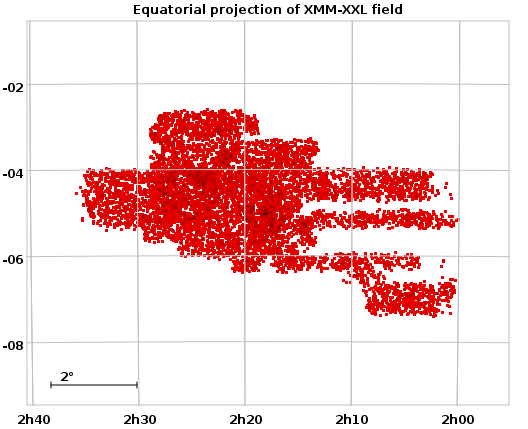
\includegraphics[scale= 0.6]{Figures/EquatorialViewXMMXXL.png}
 \caption{Ισημερινή προβολή του πεδίου \textlatin{XMM-XXL-North}. Ο οριζόντιος άξονας είναι η διορθωμένη για ιδία κίνηση ορθή αναφορά (\textlatin{RA}) και ο κατακόρυφος άξονας η διορθωμένη απόκλιση (\textlatin{Dec}). Προβάλονται οι πηγές με στοχευμένες παρατηρήσεις. (Η εικόνα παράχθηκε χρησιμοποιώντας το πρόγραμμα απεικόνισης \textlatin{TOPCAT} \cite{TopCat} και τον κατάλογο \textlatin{RapidXMM} \cite{RapidXMM}) }
 \label{fig:EquatorialView}
 \end{center}
 \end{figure}

%%%-----------------------------------------------------------%%%%
%%%-----------------------------------------------------------%%%%
%%%-----------------------------------------------------------%%%%

\section{Διαμόρφωση βάσης δεδομένων και διασταύρωση παρατηρήσεων}

%{\color{red}AGE: Επιπλεον χρειαζοτναι πληροφοριες για τον καταλογο ΧΜΜ-ΧΧ που χρησημοποιεις που δεν ειναι απο 4XMM αλλα προερχονται απο την αναλυση των https://ui.adsabs.harvard.edu/abs/2016MNRAS.459.1602L/abstract. Ισως αξιζει να πεις οι υπαρχουν πολλες διαφορετικες ομαδες που εχουν αναλυσει τα δεδομενα του ΧΜΜ στο ΧΜΜ-ΧΧΛ, αλλα εσυ επιλγεςι να χρησημοιποιησεις τον καταλογο απο το παραπανω παπερ. Ο λογος ειναι οτι για αυτο τον καταλογι εχεις στη διαθεση σου επιπλεον πληφοροφια για τις πολυχρωματρικες ιδιοτητες και την ερυθρομετατοπιση των πηγων, https://ui.adsabs.harvard.edu/abs/2017MNRAS.469.3232G/abstract. Επιπλεον θα πρεπει να αναφερθεις στο συνολικο αριθμο πηγων (π.χ. στην 0.5-2keV band, και πόσα απο αυτά εχουν φωτομετρικες και φασματοσκοπικες ερυθρομετατοπισεις.}

Τα δεδομένα του \textlatin{XMM-Newton} στο πεδίο \textlatin{XMM-XXL-North} έχουν αναλυθεί από πολλές ερευνητικές ομάδες. Εμείς επιλέγουμε να εργαστούμε με τον κατάλογο που συνοδεύει η εργασία \textlatin{<<X-ray spectral properties of the AGN sample in the northern XMM-XXL field>> (Liu et al. 2016)}\cite{2016MNRAS.459.1602L}, ο λόγος είναι ότι για τον κατάλογο αυτό έχουμε στην διάθεσή μας πληροφορία για τις πολυχρωματικές ιδιότητες και την ερυθρομετατόπιση των πηγών όπως συμπληρώνει η εργασία  \textlatin{<<X-ray constraints on the fraction of obscured active galactic nuclei at high accretion luminosities>> (Georgakakis et al. 2017)}\cite{2017MNRAS.469.3232G}.
Ο αρχικός κατάλογος αυτός έχει παρατηρήσεις από 8445 στοχευμένες πηγές. Από αυτές τις πηγές για τις 3129 έχουμε φασματοσκοπική μέτρηση ερυθρομετατόπισης, ενώ για άλλες 1854 έχουμε φωτομετρική μέτρηση ερυθρομετατόπισης (χωρίς να έχουμε φασματοσκοπική για τις τελευταίες). Έτσι από τις 8445 πηγές του αρχικού καταλόγου για τις 4983 έχουμε πληροφορία ερυθρομετατόπισης, ενώ για 3462 από αυτές δεν έχουμε καθόλου πληροφορία ερυθρομετατόπισης.

\subsection{Βάση δεδομένων \textlatin{RapidXMM}}

Για την μελέτη της μεταβλητότητας απαιτείται ένας κατάλογος που περιέχει πληροφορίες για την ένταση κάθε πηγής σε ξεχωριστές παρατηρήσεις και που περιλαμβάνει φωτομετρικές πληροφορίες για όλες τις παρατηρήσεις του \textlatin{XMM-Newton}. 
Θα χρησιμοποιήσουμε τον κατάλογο \textlatin{RapidXMM database} που συνοδεύει την εργασία \textlatin{<<The RapidXMM Upper Limit Server: X-ray aperture photometry of XMM-Newton archival observations>> (Ruiz et al. 2021)} \cite{RapidXMM}, ο κατάλογος αυτός αναπτύχθηκε για να παρέχει άνω όρια ροής για το τμήμα του ουρανού που καλύπτεται από τον \textlatin{XMM-Newton}, όμως περιλαμβάνει επιπλέον ποσότητες οι οποίες μπορούν να χρησιμοποιηθούν για τον υπολογισμό ροής (φωτομετρία) ων παρατηρούμενων πηγών. Ο κατάλογος αυτός περιέχει 63162 παρατηρήσεις από 8436 καταγεγραμμένες πηγές, σε μαλακές ($0.2-2$ \textlatin{keV}) και σκληρές ($2-12$ \textlatin{keV}) ακτίνες Χ, από τρία διαφορετικά όργανα: \textlatin{PN, MOS1, MOS2}.  
Θα επικεντρωθούμε σε στοχευμένες παρατηρήσεις του πεδίου \textlatin{XMM-XXL-North} και συγκεκριμένα σε ακτινοβολία που έχει καταγραφεί στο ενεργειακό παράθυρο $0.2-2$ \textlatin{keV}, δηλαδή ακτινοβολία μαλακών ακτίνων Χ.

Το \textlatin{RapidXMM} χρησιμοποιεί το σύστημα \textlatin{pixelisation HEALPix}, το σύστημα αυτό διαιρεί την γεωμετρική προβολή της σφαίρας σε ισεμβαδικά \textlatin{pixel} και προσφέρει μια ένα-προς-ένα απεικόνιση μιας δι-διάστατης κατανομής στοιχείων διακριτού εμβαδού σε μία μονοδιάστατη συστοιχία ακεραίων αριθμών. Η συστοιχία ακεραίων επιδέχεται δύο διαφορετικούς τρόπους αρίθμησης \textlatin{RING} και \textlatin{NESTED} καθώς και διαφορετική ευκρίνεια (μέγεθος \textlatin{pixel}). Έτσι στον θόλο προβάλεται ένα νοητό πυκνό πλέγμα που σχηματίζει <<κελιά>>. Επιλέγεται ο τρόπος αρίθμησης \textlatin{NESTED} και η παράμετρος ευκρίνειας $16$ η οποία αντιστοιχεί σε μέγεθος κελιού $3.2$ \textlatin{arcsec}, που είναι συγκρίσιμο με την ευκρίνεια των εικόνων του συστήματος \textlatin{Pipeline Processing Subsystem (PPS)} του \textlatin{XMM-Newton} οι οποίες έχουν μέγεθος \textlatin{pixel} $4.44$ \textlatin{arcsec}.\\
Για κάθε μία από αυτές τις θέσεις δίνονται μεταξύ άλλων: καταμέτρηση φωτονίων πηγής στο διάφραγμα για κάθε ενεργειακή μπάντα, καταμέτρηση φωτονίων υποβάθρου για κάθε ενεργειακή μπάντα, χρόνος έκθεσης παρατήρησης για κάθε ενεργειακή μπάντα, ανιχνευτής με τον οποίο έγινε η παρατήρηση, κλάσμα της κατανομής ροής σημειακής πηγής που περιέχεται στο διάφραγμα, ημερομηνία και ώρα έναρξης και λήξης της παρατήρησης, ο λόγος εμβαδών διαφράγματος παρατήρησης πηγής προς διάφραγμα μέτρησης υποβάθρου.

%{\color{red}AGE: ο \textlatin{RapidXMM} ειναι για τη φωτομετρια. Η αναλυση των παρατηρησεων από τοτς Liu et al., δεν περιλεμβανει πληροφορια για την μεταβλητοτα των πηγων. Οι Liu et al. συνενωσαν ολες τιςε παρατηρησεις με αλλιλοεπικαλυψη με σκοπο την αυξηση του συνολικου χρονου εκθεσης και την ανιχνευση αμυδρων πηγων. Ο καταλογος που δινει την μεση ροη καθε πηγης οπως προκυπτει απο την συννενσωη ολων των παρατηησων σε διαφορετικες εποχες (χρονικες στιγμες). Για τη μελετη της μεταβλιτοτηας απαιιητετα ενας καταλογος ο οποιος θα περιχει πληροφοριες για την ενταση καθε πηγης σε ξεχωριστες εποχες παρατηρησεις. Για το λογο αυτο χρησημοποιουμε εναν νεο καταλογο που παριλαμβανει  φωτομεττιες πληρογοριες για ολες τις ξεχωριστες παρατηρησεισ του ΧΜΜ...  Ο βασικος στοχος της αναπτηξης του \textlatin{RapidXMM} ειναι η διμιοθργια μιας βαση δεδομεμνω που θα περιεχει ανω ορια ροης σε ολο το τμημα του ουρανου που καλυπτεται απο τον ΧΜΜ. Η βαση αυτη ομως περλιμαβνει επιπλεον ποσοτητς οι οποιες μπορουν να χρησημοποιηθουν για τον υπολογιμσο της ροης πηγων (φωτομετρια). Αυτη περιλαμβανει extracted counts within an aperture of 30", the expected background level within the same aperture, the corresping expsore time...} 

%{\color{red}AGE: το \textlatin{RapidXMM} χρησημοποει το \textlatin{pixelisation HEALPix} οποτε ισως καλυτερα να το πριγραψεις εδω σε σχεση με το \textlatin{RapidXMM}. Επιπλεον πρεπει να πεις οτι η ευκερινια του  \textlatin{RapidXMM}  ειναι περιπου 3.2" που αβτιστοχει σε παράμετρο ευκρίνειας $16$. Μπορεις να πεις το \textlatin{RapidXMM} παρεχει τις παραπανω φωτομετρικες πληρογοριες σε ενα πυκνο πλεγμα (grid) απο θεσεις που αντιστοιχουν σε 3.4". Σε καθε μια απο αυτεσ τις θεσεις δινονατι οι εξεις πληροφοριες, aperture coutnts ,.... }

%%%-----------------------------------------------------------%%%%
\subsection{Αντιστοίχιση πηγών και πληροφορίες από άλλους καταλόγους}

Όπως τονίσαμε, ενώ βασιζόμαστε στις ποσότητες του καταλόγου \textlatin{RapidXMM}, χρησιμοποιούμε πληροφορίες ροής και ερυθρομετατόπισης από τον κατάλογο που συνοδεύει την εργασία \textlatin{<<X-ray constraints on the fraction of obscured active galactic nuclei at high accretion luminosities>> (Georgakakis et al. 2017)}.\\
Για να διασταυρώσουμε τις πληροφορίες αυτές με τις πηγές του \textlatin{RapidXMM}, εισάγουμε τις ουρανογραφικές (\textlatin{ICRS}) συντεταγμένες (\textlatin{RA}, \textlatin{Dec}) και μέσω του συστήματος \textlatin{HEALPix} με αρίθμηση \textlatin{pixel NESTED} και παράμετρο ευκρίνειας $16$ αντιστοιχίζουμε κάθε παρατήρηση σε έναν αριθμό ταυτοποίησης \textlatin{HEALPix}.\\
Βάσει του αριθμού αυτού, ο οποίος σηματοδοτεί μια πηγή (\textlatin{AGN}), διασταυρώνουμε παρατηρήσεις του καταλόγου \textlatin{RapidXMM database} με τις μετρήσεις ροής ενέργειας (\textlatin{flux}) και ερυθρομετατόπισης (\textlatin{redshift}). Αποτέλεσμα είναι να εμπλουτίσουμε τον κατάλογο \textlatin{RapidXMM database} με πληροφορίες για \textlatin{redshift} και \textlatin{flux} (όπου \textlatin{flux} είναι η μέση ροή κάθε πηγής που προκύπτει από όλες τις χρονικές παρατηρήσεις του \textlatin{XMM-Newton} που αντιστοιχούν σε αυτήν), όπου αυτά υπάρχουν, και να απορρίψουμε παρατηρήσεις του καταλόγου αυτού για τις οποίες δεν έχουμε τις πληροφορίες αυτές.\\
Στην εργασία αυτή θα επικεντρωθούμε σε παρατηρήσεις του ανιχνευτή ΡΝ σε μαλακές ακτίνες Χ (δηλαδή στο ενεργειακό παράθυρο $0.2-2$ \textlatin{keV}).
Ο κατάλογος \textlatin{RapidXMM} περιέχει 8436 πηγές (από τις 8445 του αρχικού καταλόγου) από τις οποίες οι 8299 έχουν παρατηρήσεις από τον ανιχνευτή ΡΝ. Από τις 8299 πηγές αυτές οι 3092 έχουν μέτρηση φασματοσκοπικής ερυθρομετατόπισης, ενώ άλλες 1830 έχουν φωτομετρική μέτρηση ερυθρομετατόπισης. Δηλαδή από τις 8299 πηγές με παρατηρήσεις στον ανιχνευτή ΡΝ του καταλόγου \textlatin{RapidXMM database} για τις 4922 έχουμε πληροφορία ερυθρομετατόπισης, ενώ για τις 3377 δεν έχουμε πληροφορία ερυθρομετατοπισης.

%{\color{red}AGE: οι πηγες προεχρονται απο τον καταλογο των \textlatin{Liu et al. 2016} και οχι απο το  \textlatin{4XMM-DR9}. Επιπλεον η φωτομετρια δεν τατθοποιεις τις πηγες με τη ροη απο το 4ΧΜΜ αλλα αντιθετα υπολογιζεις τη φωτομετρια απο το ραπιδ. Εδω περιγραφεις πως κανεις query με ra, dec ωστε να βρεις τα αντιστοιχα \textlatin{HEALPix} πιξελ πανω στα οποια βρισκονταο οι πηγες. Εαν μια πηγη εχει παρτηρηθεο σε περισσιτερες απο μια ξεχωριστες ΧΜΜ-Νεςτον παρατηρησεις η βαση δεδοεμενων  \textlatin{RapidXMM}  επιστρεφει για καθε μια απο τις αυτες: (α) συνολικο αριθμο από φωτονια σε καθε μια απο τις πανρες .... (β) .... (γ)....  Οι τιμες αυτες ειναι δυνατο να συνδιαστουν για τον υπολογισμο της παρατηρουμενης ροης της πηγης σε ξαθε ξεωχιστη παρατηρση. Επισης μπορεις να πεις εδω οτι χρησημοποιεις μονο PN kai 0.2-2keV.}

%%%-----------------------------------------------------------%%%%
%%%-----------------------------------------------------------%%%%
%%%-----------------------------------------------------------%%%%
\section{Υπολογισμός ποσοτήτων}

%{\color{red}AGE: Ισως θα μπορουσες να ξεινησεις απο την φωτομετρια της CR=(N-B)/t/EEF, Εξηγεις τη ειναι η καθε μια ποσοτητα. Στηη συνεχεια εξηγεις πως υπολογιζεται το Β, και μονο τοτε αναφρεις την προσσεγιση dB=sqrt(B) και εξηγεις οτι η κατανομη ειναι Poisson. Επισης στη συνεχεια και την αβεβαιοτητα. Επισης πρεπει να πεις οτι το CR εχει μοναδες photo/s kai oxi erg/s/cm2 (energy flux) και συνεπως δεν περιλμαβνει υποθεσεις για το φασμα της πηγης.}

\subsection{\textlatin{Count rate} και αβεβαιότητα}

Για την φωτομετρία στις ακτίνες Χ, ως ροή δεν χρησιμοποιούμε το μέγεθος της ενεργειακής ροής (\textlatin{flux}) που μετράται σε \textlatin{erg s}$^{-1}$ \textlatin{cm}$^{-2}$, αλλά χρησιμοποιούμε το μέγεθος του ρυθμού καταγραφής φωτονίων (\textlatin{count rate}) που μετρά φωτόνια (κυματοπακέτα) ανά μονάδα χρόνου \textlatin{photon counts} $\cdot$ \textlatin{s}$^{-1})$. Το μέγεθος αυτό είναι καθαρά φωτομετρικό και δεν περιλαμβάνει καμία παραδοχή για το φάσμα της πηγής.\\
Όπως είδαμε και στην ενότητα 3.7.3, οι παρατηρήσεις των πηγών που μελετάμε έγιναν με άνοιγμα διάφραγματος ακτίνας $15$ \textlatin{arcsec} ενώ για την καταγραφή του υποβάθρου το άνοιγμα του διαφράγματος είναι δακτύλιος μεταξύ ακτίνων $60$ και $180$ \textlatin{arcsec}.

To \textlatin{Count Rate} για κάθε παρατήρησή μας δεδομένης ενεργειακής μπάντας (εδώ $0.2-2$ \textlatin{keV}) και για δεδομένο όργανο παρατήρησης (εδώ \textlatin{EPIC PN})\cite{RapidXMM}:
\begin{equation} CR = \frac {(T-B)} { t_{exp}  \cdot EEF}  \label{eq:CR} \end{equation}

Όπου:\\
$T$ : η συνολική καταμέτρηση φωτονίων (\textlatin{total realised counts}) στο διάφραγμα ($15$ \textlatin{arcsec} για στοχευμένες παρατηρήσεις)\\ 
$B$ : υπόβαθρο (\textlatin{background})\\
$t_{exp}$ : χρονικό διάστημα διάρκειας μεμονομένης παρατήρησης \\
$\mbox{EEF}$ : κλάσμα ενέργειας της \textlatin{PSF} της παρατήρησης που περικλείεται στο διάφραγμα ακτίνας $15$ \textlatin{arcsec}

Η αβεβαιότητα στον υπολογισμό $CR$ για κάθε παρατήρηση εκτιμάται σύμφωνα με την διάδοση σφαλμάτων\cite{BuchnerGeorgakakis} (αν θεωρήσουμε το $CR$ ως συνάρτηση των μεταβλητών $Τ$ και $Β$, $CR(T,B) = \frac {(T-B)} { t_{exp}  \cdot EEF} $):     
  \begin{equation} CR_{err} = \sqrt{ \Big( \frac{\partial CR}{\partial T} \Big)^2 \cdot T_{err}^2  +  \Big( \frac{\partial CR}{\partial B} \Big)^2 \cdot B_{err}^2   } = \frac{1}{t_{exp} \cdot EEF} \sqrt{  T_{err}^2 + B_{err}^2    } \label{eq:CRerr} \end{equation}
  
Όπου:\\
$T_{err} = \delta T$ : η αβεβαιότητα στην συνολική καταμέτρηση φωτονίων (\textlatin{total realised counts}) στο διάφραγμα ($15$ \textlatin{arcsec} για στοχευμένες παρατηρήσεις)\\ 
$B_{err} = \delta B$ :  η αβεβαιότητα στo \textlatin{background} (θα συζητηθεί παρακάτω)

Για να υπολογίσουμε την στατιστική αβεβαιότητα στα \textlatin{total realised counts} θα χρησιμοποιήσουμε την προσέγγιση \textlatin{Gehrels}\cite{1986ApJ...303..336G}.
\begin{equation} \delta T \approx 1+\sqrt{T+0.75 } \label{eq:Gehrels} \end{equation}
Η προσέγγιση αυτή είναι χρήσιμη για υπολογισμό άνω ορίων διαστήματος αξιοπιστίας σε περιπτώσεις μικρού πλήθους γεγονότων (π.χ. μικρό πλήθος καταγεγραμμένων φωτονίων) στατιστικού δείγματος.

Η παραπάνω έκφραση για τον ρυθμό καταγραφής φωτονίων (εξίσωση \ref{eq:CR}) προκύπτει επειδή (αν $S$ to σήμα της πηγής) η συνεισφορά του σήματος της πηγής στο πλήθος παρατηρούμενων φωτονίων στο διάφραγμα εξαρτάται από το σχήμα της \textlatin{PSF} και από τον χρόνο παρατήρησης. Αν το εγγενές \textlatin{Count Rate} μιας πηγής είναι $CR$, τότε το σήμα πηγής $S$\cite{RapidXMM}:
\begin{equation}
    S = CR \cdot t_{exp}  \cdot EEF \label{eq:sourcesignal}
\end{equation}
Ο καταγραφόμενος αριθμός φωτονίων $T$ στο διάφραγμα είναι υλοποίηση μιας διαδικασίας \textlatin{Poisson}, με αναμενόμενη τιμή $\lambda = S + B$.   

%%%-----------------------------------------------------------%%%%

\subsection{Ακτινοβολία υποβάθρου και αβεβαιότητα}

Η καταγραφή και καταμέτρηση φωτονίων (γεγονότων) και ο υπολογισμός του ρυθμού πραγματοποίησης των γεγονότων αυτών διέπονται από στατιστική \textlatin{Poisson}. Όταν έχουμε σχετικά υψηλό αριθμό γεγονότων, τότε έχουμε αντιστοίχηση με στατιστική \textlatin{Gauss} (για περισσότερα γεγονότα έχουμε αντιστοίχιση σε περισσότερα $\sigma$)\cite{1986ApJ...303..336G}. Για να εκτιμήσουμε το υπόβαθρο, καταγράφουμε φωτόνια σε μεγαλύτερο διάφραγμα και έπειτα τα συρρικνώνουμε με τον λόγο των εμβαδών των διαφραγμάτων. Στην βάση δεδομένων μας, διαθέτουμε το κλάσμα φωτονίων υποβάθρου που αντιστοιχεί στην παρατήρηση και τον λόγο εμβαδών, έτσι συμπεραίνουμε το υπόβαθρο στην συλλογή μεγάλου διαφράγματος (χρησιμοποιώντας όλην την πληροφορία που συλλέχθηκε) και υπολογίζουμε την αβεβαιότητα με καλή προσέγγιση στατιστικής \textlatin{Gauss}, έπειτα χρησιμοποιώντας τον λόγο των εμβαδών εκτιμούμε την αβεβαιότητα στην κλίμακα της παρατήρησης.
Το ανηγμένο υπόβαθρο $B_{poisson}$:
\begin{equation}
    B_{Rapid} = B_{poisson}  \cdot \frac {A_{source} }{A_{backgr}} \iff B_{poisson} =   \dfrac{ B_{Rapid} }{\frac {Α_{source} }{Α_{backgr}} } \label{eq:Background}
\end{equation}
H αβεβαιότητα ανηγμένου υποβάθρου στην προσέγγιση \textlatin{Gauss} $\delta B_{poisson}$:
\begin{equation}
     \delta B_{poisson} = \sqrt{ B_{poisson}} =\sqrt{ \dfrac{ B_{Rapid} }{\frac {Α_{source}}{Α_{backgr}} }}
\end{equation}
H αβεβαιότητα στο διάφραγμα της παρατήρησης, από την αβεβαιότητα ανηγμένου υποβάθρου:
\begin{equation}
     \delta B_{Rapid} = \delta B_{poisson} \cdot \frac {A_{source} }{A_{backgr}}= \sqrt{ \dfrac{ B_{Rapid} }{\frac {Α_{source}}{Α_{backgr}} }}\cdot \frac {A_{source} }{A_{backgr}} \label{eq:Berr}
\end{equation}
%%%-----------------------------------------------------------%%%%

\subsection{\textlatin{Signal-to-Noise ratio} }
Για κάθε μια παρατήρηση ο λόγος σήματος προς θόρυβο \textlatin{Signal-to-Noise ratio (S/N)}:   
\begin{equation}   S/N = \frac{T-B}{\sqrt{\delta T^2 + \delta B^2}} \end{equation}
Όπου:\\     
$T$ :  η συνολική καταμέτρηση φωτονίων (\textlatin{total realised counts}) στο διάφραγμα \\
$B$ : \textlatin{background}  \\   
$\delta T$ : η αβεβαιότητα στα \textlatin{total realised counts} (Βλ. εξίσωση \ref{eq:Gehrels})\\
$\delta B$ : η αβεβαιότητα στο \textlatin{background} (Βλ. εξίσωση \ref{eq:Berr})

Έτσι για κάθε μία παρατήρηση κάθε πηγής μπορούμε να έχουμε και μια τιμή \textlatin{S/N}.
Ενώ μπορούμε σε κάθε μία πηγή (\textlatin{HEALPix ID}) να αναθέσουμε μία συσσωρευμένη τιμή \textlatin{S/N} συγκεντρώνοντας τις μετρήσεις όλων των παρατηρήσεων που αντιστοιχούν σε κάθε πηγή ως εξής:
 \begin{equation} {S/N}_{stacked} =   \dfrac { \sum_1^N T_i -  \sum_1^N  B_i}{\sqrt{ \big(\sum_1^N \delta T_i \big)^2 + \big(\sum_1^N \delta B_i \big)^2}} \label{eq:SNstacked}\end{equation} 
 
Στο εξής όταν αναφερόμαστε σε τιμή \textlatin{S/N} μίας πηγής, θα αναφερόμαστε στον υπολογισμό της εξίσωσης \ref{eq:SNstacked}.
   
%%%-----------------------------------------------------------%%%%
\subsection{\textlatin{Νormalised Excess Variance} και αβεβαιότητα }

H \textlatin{excess variance (NXSV)} μετρά πόση από την ολική ροή είναι μεταβλητή, αφού αφαιρέσουμε το στατιστικό σφάλμα. Το \textlatin{Count Rate (CR)} είναι υποτυπώδης ροή ως ρυθμός καταμέτρησης φωτονίων. Χρησιμοποιώντας τον παρακάτω τύπο, υπολογίζουμε για κάθε πηγή- δηλαδή για κάθε ξεχωριστό αριθμό \textlatin{HEALPix}- την ποσότητα \textlatin{NXSV} για παρατηρήσεις στην ενεργειακή μπάντα $0.2-2$ \textlatin{keV} \cite{1997ApJ...476...70N}: 
    \begin{equation} \sigma^2_{rms} = \frac{1}{N \cdot {\bar x}^2 }   \sum_{i=1}^{N}  [ (x_i -\bar x)^2  - x_{err, i}^2]  \label{eq:NXSV}\end{equation}
Όπου:\\
$N$ : πλήθος παρατηρήσεων που αντιστοιχούν σε μία πηγή \\                              
$x_i$ : \textlatin{Count Rate} μιας μεμονομένης παρατήρησης \\             
$\bar x$ : αριθμητικός μέσος όρος \textlatin{Count Rate} από παρατηρήσεις που αντιστοιχούν σε μία πηγή\\ 
$x_{err, i}$ : στατιστικη αβεβαιότητα στο \textlatin{Count Rate} μιας μεμονομένης παρατήρησης (όπως την υπολογίσαμε σε παραπάνω ενότητα, εξίσωση \ref{eq:CRerr} )  %{\color{red}(δωσε τον αριθμο του equation) λογω του σφαλμαοτς μετησεις}\\

Η αβεβαιότητα στην \textlatin{NXSV} ($\sigma^2_{rms}$) είναι $  \sigma^2_{rms, err}$, αναπαριστά τα σφάλματα μέτρησης σε εκτιμήσεις της \textlatin{NXSV} από προσομοιώσεις καμπύλων φωτός και υπολογίζεται από την εξής εμπειρική σχέση\cite{2003MNRAS.345.1271V}:     
  
\begin{equation}  \sigma^2_{rms, err} = \sqrt{ \Big( \sqrt{\frac{2}{N}}\cdot \frac{\overline{ x^2_{err} }}{\bar{x}^2} \Big)^2 + \Big( \sqrt{ \frac{\overline{ x^2_{err}}}{N}    }   \cdot \frac{2F_{var}}{\bar x}  \Big)^2  }  \label{eq:NXSVerr} \end{equation}

$N$ : πλήθος παρατηρήσεων που αντιστοιχούν σε μία πηγή \\
Όπου η ποσότητα $\overline{ x^2_{err}}$ είναι η μέση τετραγωνική αβεβαιότητα στο \textlatin{Count Rate}:     
\begin{equation}  \overline{ x^2_{err}} =   \frac{1}{N }   \sum_{i=1}^{N} x_{err, i}^2  \end{equation}
 
Και η ποσότητα $F_{var} $ είναι το κλασματικό πλάτος της \textlatin{NXSV}:    
\begin{equation} F_{var} = \sqrt{ \frac{ \sigma^2_{rms} -  \overline{ x^2_{err}}   } {{\bar x}^2}  }     \end{equation}
Έτσι, η κάθε μέτρηση \textlatin{NXSV} για κάθε πηγή συνοδεύεται με τον αντίστοιχο υπολογισμό για την αβεβαιότητα της \textlatin{NXSV}.

  \begin{figure*}
 \begin{center}
 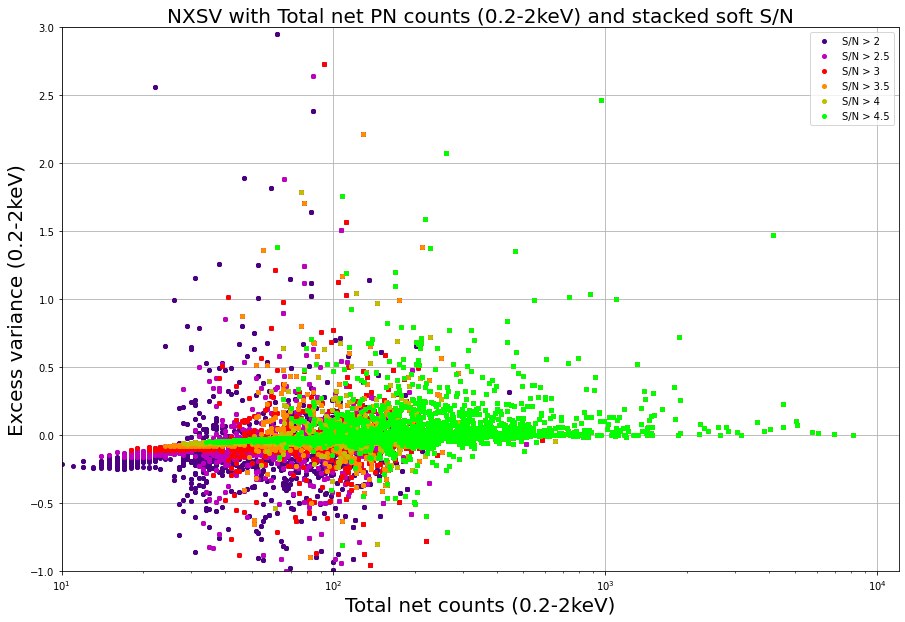
\includegraphics[width=0.9\linewidth]{Figures/NXSV_Counts_zweight.png}
 \caption{\textlatin{NXSV} με συνολικές καταμετρήσεις φωτονίων στο διάφραγμα κατά \textlatin{redshift.}}
 \label{fig:NXSV_counts}
 \end{center}
 \end{figure*}

Όπως βλέπουμε στην εξίσωση \ref{fig:NXSV_counts}, στούς υπολογισμούς μας έχουμε τιμές της \textlatin{NXSV} οι οποίες είναι αρνητικές, αυτό συμβαίνει διότι όπως φαίνεται στον τύπο \ref{eq:NXSV}, η τετραγωνική αβεβαιότητα μεμονομένων παρατηρήσεων \textlatin{CR} είναι μεγαλύτερη από το τετράγωνο της απόστασής τους από την μέση τιμή των παρατηρήσεων της πηγής στην οποία αντιστοιχούν. Όπως βλέπουμε στο σχήμα \ref{fig:NXSV_counts} αυτό αντιμετωπίζεται σε μεγάλο βαθμό αν απορρίψουμε πηγές με μικρό \textlatin{S/N}, καθώς ο θόρυβος σήματος συνεισφέρει σημαντικά στην αβεβαιότητα της μέτρησης. 

%%%-----------------------------------------------------------%%%%
\subsection{Λαμπρότητα και \textlatin{redshift}}

Έχοντας πληροφορίες για ερυθρομετατόπιση και ροή στην ενεργειακή μπάντα $0.2-2$ \textlatin{keV} \cite{2017MNRAS.469.3232G}, υπολογίζουμε απόσταση και λαμπρότητα για κάθε μία πηγή (\textlatin{AGN})\cite{2006PASP..118.1711W}. Χρησιμοποιούμε τις κοσμολογικές παραμέτρους $H_0 = 70$ \textlatin{km  s}$^{-1}$ \textlatin{Mpc}$^{-1}$, $\Omega_m = 0.3$ , $\Omega_v=0.7$ και επίπεδο Σύμπαν.\\
Για δεδομένο \textlatin{redshift}, $z$, ο παράγοντας κλίμακας του Σύμπαντος:   $a = \dfrac{1}{1+z}$\\
Η αδρανειακή ακτινική απόσταση (\textlatin{comoving radial distance}- απόσταση που μετράμε στο αδρανειακό μας σύστημα ως παρατηρητές)\cite{2006PASP..118.1711W}:
\begin{equation}
D_{cmr} =  \int \frac{c dt}{a} = \int_{1/(1+z)}^1 \frac {cda}{a\dot a}
\end{equation}

Η απόσταση που διανύει το φώς (\textlatin{light travel time distance}- χρόνος φωτός από την εκπομπή του μέχρι την καταγραφή του σήματος)\cite{2006PASP..118.1711W}:
\begin{equation} D_{ltt} =  \int c dt = \int_{1/(1+z)}^1 \frac {cda}{\dot a} \end{equation}

Θεωρούμε ποσότητα $X$ τέτοια ώστε: \begin{equation} \dot a = H_o \sqrt X \end{equation}
Για επίπεδο Σύμπαν ($\Omega_{tot}=1$), με $\Omega_m$, $\Omega_v$ (ύλη και κενό μόνο) η ποσότητα αυτή γίνεται:    
\begin{equation} X(a) = \frac{\Omega_m}{a} + \frac{\Omega_r}{a^2} + \Omega_{v} a^2 + (1-\Omega_{tot}) \iff X(a) = \frac{\Omega_m}{a} + \Omega_v a^2 \end{equation}  

Έτσι, η αδρανειακή ακτινική απόσταση:
\begin{equation} 
\begin{aligned}
D_{cmr} =  {} &  \int_{1/(1+z)}^1 \frac {c }{a\cdot H_o \sqrt X} da = \frac{c}{H_o}  \int_{z}^0  (1+z) \cdot \frac{1}{\sqrt{\Omega_m/a + \Omega_v a^2 }} d \big( \frac{1}{1+z} \big) = \\
& =\frac{c}{H_o}  \int_{z}^0  \frac{(1+z)}{\sqrt{\Omega_m/a + \Omega_v a^2 }} \Big( \frac{-1}{(1+z)^2} \Big) dz = % \end{equation}
%\begin{equation} =  
\frac{c}{H_o}  \int_0^{z} \frac{1}{(z+1) \sqrt{\Omega_m/a + \Omega_v a^2 }} dz = \\ & =\frac{c}{H_o}  \int_0^{z} \frac{1}{(z+1) \sqrt{\Omega_m (1+z) + \Omega_v / (1+z)^2 }} dz \label{eq:Dcmr}
\end{aligned}
\end{equation}

Η απόσταση γωνιακής διαμέτρου $ D_{A} = \frac{R}{\theta}$ (\textlatin{angular size distance}- το εγκάρσιο ιδιομήκος $R$ ένος αντικειμένου που υποτείνει γωνία $\theta$):
 $D_{A} =  \frac{D_{cmr}}{(1+z)}  $

Η απόσταση λαμπρότητας (\textlatin{luminosity distance}- ορίζεται ώστε ο νόμος αντιστρόφου τετραγώνου για βολομετρικές ροές $F_{bol} = L/(4\pi D_L^2)$ να λειτουργεί πλήρως)\cite{2006PASP..118.1711W}: 
\begin{equation}  D_L = (1+z)^2 D_A = (1+z) D_{cmr} \label{eq:DL}\end{equation}

Έτσι, σύμφωνα με τον παραπάνω τύπο και τις κοσμολογικές παραδοχές μας, αρκεί να γνωρίζουμε το $z$ μιας πηγής και να εκτιμήσουμε αριθμητικά το ολοκλήρωμα στην έκφραση $D_{cmr}$ για να υπολογίσουμε την απόσταση λαμπρότητας $D_L$ για κάθε \textlatin{AGN} που μελετάμε.
Έπειτα χρησημοποιούμε την σχέση ροής-λαμπρότητας για το φάσμα των μαλακών ακτίνων $X$:
\begin{equation}L_{X,obs} = 4\pi D_L^2 F_{X,obs} \label{eq:LumiFluxObs}\end{equation}
Όπου $F_{X,obs}$ είναι η παρατηρούμενη ροή στο αδρανειακό μας σύστημα. Για πηγή με ερυθρομετατόπιση $z$ φωτόνιο που παρατηρείται να έχει συχνότητα $\nu_{obs}$ έχει εκπεμφθεί από την πηγή στο σύστημα ηρεμίας της με συχνότητα $\nu_{rest}$ me $\nu_{rest} = (1+z)\nu_{obs}$. Δηλαδή η παρατηρούμενη συχνότητα είναι σε χαμηλότερη ενέργεια από την εκπεμπόμενη\cite{2002astro.ph.10394H}.\\
Η ολοκληρωμένη ροή που παρατηρούμε και καταγράφουμε στην ενεργειακή μπάντα $0.2-2$ \textlatin{keV} είναι $F_{X,obs}$ ένω η αντίστοιχή της ολοκληρωμένη ροή ηρεμίας της πηγής είναι $F_{X,rest}$.
Διορθώνουμε λοιπόν την παρατηρούμενη λαμπρότητα $L_{X,obs}$ με τον λόγο της ροής στο εύρος ενεργειών του συστήματος ηρεμίας της πηγής προς την ροή στο εύρος ενεργειών του συστήματος παρατήρησης \textlatin{(K-correction)} \cite{1998ApJ...495..100J}: 
\begin{equation}Κ_{0.2-2} =\dfrac{F_{X,obs}}{F_{X,rest}} =\dfrac{\int_{0.2}^{2} h\nu \cdot f(h\nu) d(h\nu)}{\int_{0.2(1+z)}^{2(1+z)}h\nu\cdot f(h\nu) d(h\nu)}\label{eq:K-correction ratio}\end{equation}  
Όπου $h$ η σταθερά \textlatin{Planck}, $\nu$ η συχνότητα φωτεινού σήματος, $f(h\nu)$ η συνάρτηση ροής με ενέργεια φωτονίου. Σε mia πρώτη προσέγγιση η ροή εξαρτάται από την συχνότητα wς νόμος δύναμης με φασματικό δείκτη $\alpha = 1.9$, δηλαδή $f(h\nu) = A \cdot \nu^{-1.9}$ με $Α$ κάποια σταθερά. Τότε ο λόγος \textlatin{K-correction} γίνεται:
\begin{equation} \begin{aligned} Κ_{0.2-2} =  {} & \dfrac{\int_{0.2}^{2} A \cdot \nu \cdot \nu^{-1.9} hd\nu}{\int_{0.2(1+z)}^{2(1+z)}A \cdot \nu \cdot \nu^{-1.9} hd\nu} =  \dfrac{\int_{0.2}^{2} A  \cdot \nu^{-0.9} hd\nu}{\int_{0.2(1+z)}^{2(1+z)}A  \cdot \nu^{-0.9} hd\nu}
\\  & \dfrac{(2)^{1-0.9}-(0.2)^{1-0.9}}{(2(1+z))^{1-0.9}-(0.2(1+z))^{1-0.9}}=\\ & = \dfrac{(2)^{1-0.9}-(0.2)^{1-0.9}}{(1+z)^{1-0.9}\cdot[(2)^{1-0.9}-(0.2)^{1-0.9}]} = \dfrac{1}{(1+z)^{0.1}} \label{eq:K-correction}\end{aligned}\end{equation}
Έτσι ο λόγος  ${F_{X,obs}}/{F_{X,rest}} = (1+z)^{-0.1} \iff {F_{X,rest}} = (1+z)^{0.1} {F_{X,obs}} $, έχοντας κάνει την προσέγγιση νόμου δύναμης με φασματικό δείκτη $\alpha = 1.9$.
Για την λαμπρότητα της πηγής στο αδρανειακό σύστημα ηρεμίας της έχουμε:
\begin{equation}L_{X,rest} = 4\pi D_L^2 F_{X,rest} = 4\pi(1+z)^{0.1} D_L^2 F_{X,obs} \label{eq:LumiFluxRest}\end{equation} 
Με τον τρόπο αυτό έχουμε πληροφορία της πραγματικής (στο σύστημα ηρεμίας της πηγής) λαμπρότητας κάθε πηγής στην παρατηρούμενη ενεργειακή μπάντα $0.2-2$ \textlatin{keV}, για τις πηγές για τις οποίες έχουμε είτε φωτομετρικό είτε φασματοσκοπικό \textlatin{redshift}. Η εξάρτηση λαμπρότητας- \textlatin{redshift} φαίνεται στο σχήμα \ref{fig:LumiRed}, ενώ παρατηρούμε ότι οι πηγές με μεγαλύτερη λαμπρότητα είναι αυτές με τις μεγαλύτερες τιμές \textlatin{redshift} (σχήμα \ref{fig:NXSV-Zcbar}).
%{\color{red} the equation above is missing the k-correction. }

 \begin{figure*}
 \begin{center}
 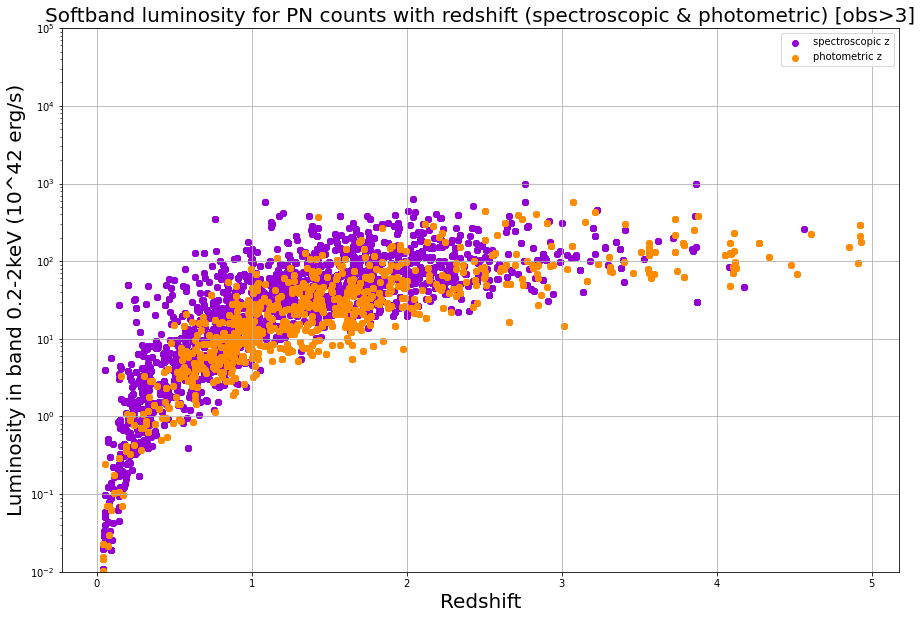
\includegraphics[width=0.8 \linewidth]{Figures/Lumi_Red.png}
 \caption{Λαμπρότητα ($ 10^{42}$ \textlatin{erg s}$^{-1}$) στις μαλακές ακτίνες Χ ($0.2-2$ \textlatin{keV}) συναρτήσει του \textlatin{redshift.}}
 \label{fig:LumiRed}
 \end{center}
 \end{figure*}
 
 
\begin{figure*}%
    \centering
    \subfloat{{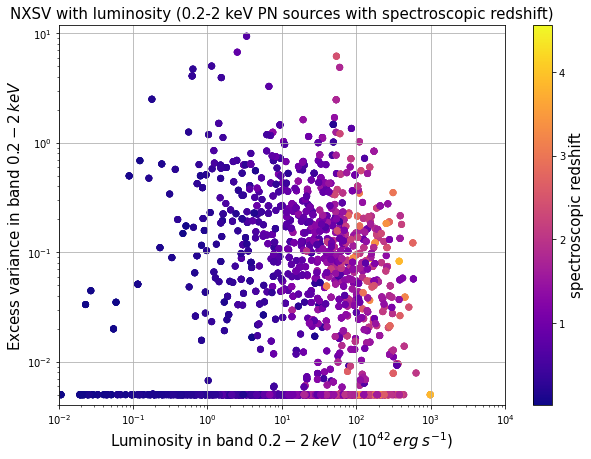
\includegraphics[width=0.9\linewidth]{Figures/NXSV_Lumi_zweight_SPECTRO.png} }}%
    \qquad
    \subfloat{{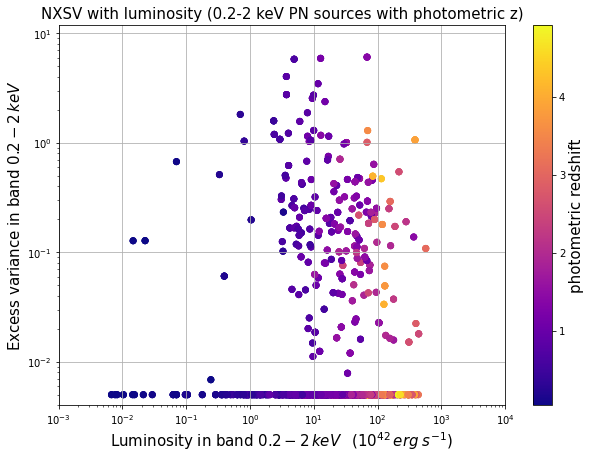
\includegraphics[width=0.9\linewidth]{Figures/NXSV_Lumi_zweight_PHOTO.png} }}%
    \caption{ \textlatin{NXSV} με λαμπρότητα κατά \textlatin{redshift.} Στο πάνω πάνελ οι πηγές για τις οποίες έχουμε φασματοσκοπική μέτρηση ερυθρομετατόπισης, ενώ στο κάτω πηγές για τις οποίες έχουμε μόνο φωτομετρική μέτρηση ερυθρομετατόπισης. Οι πηγές με \textlatin{NXSV}$<0.005$ απεικονίζονται στο επίπεδο 0.005.} \label{fig:NXSV-Zcbar}
\end{figure*}
%%%-----------------------------------------------------------%%%%
%%%-----------------------------------------------------------%%%%
%%%-----------------------------------------------------------%%%%

\section{Περιορισμός δείγματος και ανάλυση δεδομένων}

%{\color{red}: better to give values in years. Also wht you split them into near-equal time invtervals: Σκοπος είναι να μελετησουμε τη μεταβλοτητα των ΕΝΠ σε να χρονικο διαστημα 20 χρονων. Για το σκοπο αυτο διαλεγουμε πηγες που εχουν καμπλυλες φωτος με ομιομορφο sampling κατα τη διαρκεια των 19 χρονων κατα το οποιο το ΧΜΜ-ΧΜΛ εχει παρατηρηθει. Για το σκοπο αυτο χωριζουμε το συνολικο αριθμο παρτηρησεων σε 3 ομαδες οι ιποιες διαχωριζονται μεταξυ τους απο περιπου 4-5 ετη. Οι περιοδοι αυτοί αντιστοιχούν χονδιρκα στις 3 κυριες περιοδους κατα τις οποίες το ΧΜΜ-ΧΧΛ παρτηρηθηκε απλο το ΧΜΜ ωσ αποτελεσμα 3 μεγαωλων προγραμματων: XMM-XXL (arxes 2000, Pierre et al. 2006.), XMM-XXL (~2010) kai XMM Serves (telos tis dekaeties 2010. Απαιτουμε οι πηγες για τις οποιες θα υπολογισουμε ... να εχουνε τουλαχιστον μια παρατησρηση και στις 3 παραπακνβ περιοδουςσ....}. 
Θεωρούμε ότι η εγγενής μεταβλητότητα, την οποία εκτιμάμε με την $\sigma_{rms}^2$, είναι μια στοχαστική διαδικασία - έχει δηλαδή χαρακτήρα <<κόκκινου θορύβου>> \textlatin{(red noise)}. Τότε η \textlatin{NXSV} εξαρτάται από την διάρκεια της καμπύλης φωτός στο σύστημα ηρεμίας της πηγής. Καμπύλες φωτός πολύ μικρές σε έκταση κυριαρχούνται από στατιστικό θόρυβο και έτσι δεν είναι πολύ χρήσιμες στην μελέτη μας\cite{2017MNRAS.471.4398P}.\\
Οι συνολικές παρατηρήσεις όλων των πηγών εκτείνονται σε 19 έτη ($\sim 600$ \textlatin{Ms}). Σκοπός μας είναι να μελετήσουμε καμπύλες φωτός που να εκτείνονται σε όλο αυτό το χρονικό διάστημα (δηλαδή η κλίμακα χρόνου της εκτίμησης μεταβλητότητας είναι $\sim 10-20$ έτη) και τα σημεία τους να είναι όσο το δυνατόν ομοιόμορφα κατανεμημένα στην χρονοσειρά. Όμως, στον πλήρη πληθυσμό του πεδίου \textlatin{XMM-XXL-North} δεν έχουμε καμία καμπύλη φωτός μεμονομένης πηγής με περισσότερα από 15 σημεία από τον ανιχνευτή ΡΝ.\\
Για να εκλέξουμε όσο το δυνατόν μεγαλύτερες καμπύλες φωτός ομοιόμορφης συλλογής, χωρίζουμε τις συνολικές παρατηρήσεις σε τρεις εποχές- τρία χρονικά διαστήματα των 6-7 περίπου ετών ($\sim 200 $\textlatin{ Ms}) έκαστο. Ξεχωρίζουμε, λοιπόν, αφού έχουμε μετατρέψει τις χρονικές στιγμές έναρξης και λήξης κάθε παρατήρησης σε Ιουλιανή Εποχή (\textlatin{Julian Epoch}), τις εξής εποχές: 
\begin{itemize}
    \item Εποχή 1: [2000.0,2006.0] εκτείνεται σε 6 έτη, $\sim 189$ \textlatin{Ms}
    \item Εποχή 2: (2006.0,2014.0] εκτείνεται σε 8 έτη, $\sim 252$ \textlatin{Ms}
    \item Εποχή 3: (2014.0,2020.0] εκτείνεται σε 7 έτη, $\sim 221$ \textlatin{Ms}
\end{itemize}

Οι περίοδοι αυτές αντιστοιχούν σε αδρές γραμμές στις 3 κύριες περιόδους κατά τις οποίες το πεδίο \textlatin{XMM-XXL-North} παρατηρήθηκε από το τηλεσκόπιο \textlatin{XMM-Newton} ως αποτέλεσμα 3 μεγάλων προγραμμάτων: \textlatin{XMM-LSS} (αρχές 2000, \cite{2006MNRAS.372..591P}), \textlatin{XMM-XXL} ($\sim$2010, \cite{2016A&A...592A...1P}) kai \textlatin{XMM-SERVS} (προς το τέλος της δεκαετείας 2010, \cite{2018MNRAS.478.2132C}).

\begin{figure*} 
 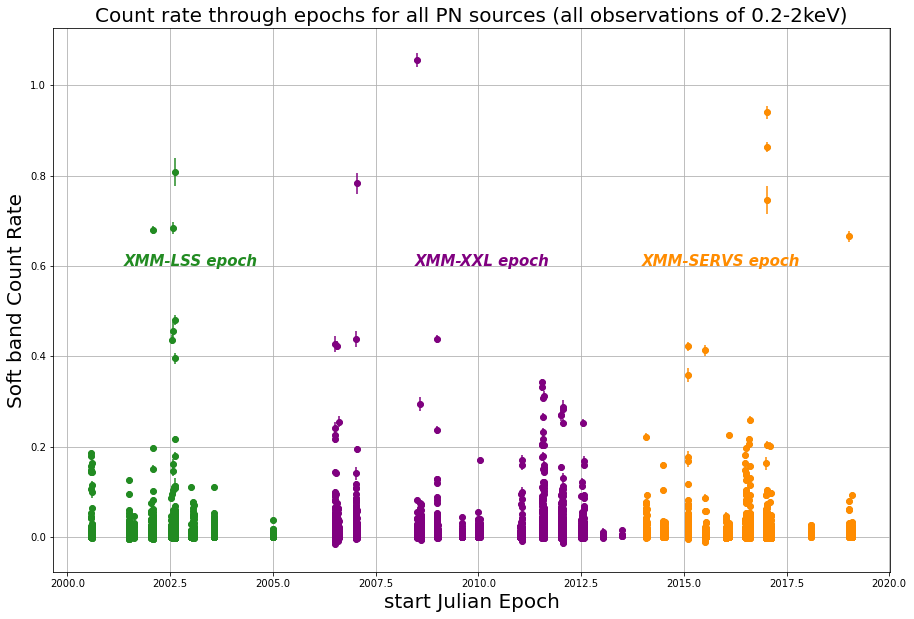
\includegraphics[width=0.9\linewidth]{Figures/Epochs.png}
 \caption{Οι συνολικές παρατηρήσεις εμπίπτουν σε τρία χρονικά διαστήματα- εποχές. Εδώ ο ρυθμός καταμέτρησης (\textlatin{CR}) με την χρονική τοποθέτηση της έναρξης κάθε παρατήρησης του ανιχνευτή \textlatin{PN} στην ερνεργειακή μπάντα $0.2-2$ \textlatin{keV}. }
 \label{fig:Epochs}
 \end{figure*}
 
Περιορίζουμε το δείγμα μας σε πηγές που έχουν παρατηρήσεις από τον ανιχνευτή \textlatin{PN} σε τρείς διαδοχικές διαφορετικές εποχές (όπως φαίνονται στο σχήμα \ref{fig:Epochs}), δηλαδή επιλέγουμε τις πηγές που έχουν μία τουλάχιστον παρατήρηση σε κάθε ένα από τα χρονικά διαστήματα που ορίσαμε, ετσι ώστε το δείγμα μας να έχει συνεχείς χρονικά παρατηρήσεις για μεγάλο χρονικό διάστημα. Η καμπύλη φωτός με το μεγαλύτερο παρατηρούμενο μήκος καλύπτει περίπου $17$ έτη, ενώ το μέσο μήκος καμπύλης φωτός καλύπτει $11$ έτη- αυτές είναι και οι χρονικές κλίμακες ($\sim 400$ \textlatin{Ms}) στις οποίες μελετάμε την μεταβλητότητα. 

Έχοντας επιλέξει πηγές με παρατηρήσεις σε τρείς διαδοχικές εποχές στην ενεργειακή μπάντα $0.2-2$ \textlatin{keV} από τον ανιχνευτή \textlatin{PN}, προκειμένου να αποκλείσουμε πηγές που έχουν πολύ θόρυβο (δηλαδή μικρό λόγο \textlatin{S/N}) επιλέγουμε να κάνουμε τα γραφήματα της  \textlatin{NXSV} με λαμπρότητα για πηγές με \textlatin{S/N}$>2$, \textlatin{S/N}$>3$, \textlatin{S/N}$>4$ (επιλέγοντας να βάλουμε ένα κάτω φραγμό στο \textlatin{S/N} του δείγματός μας, όπως φαίνεται στο σχήμα \ref{fig:NXSV_counts}).

 \begin{figure*}  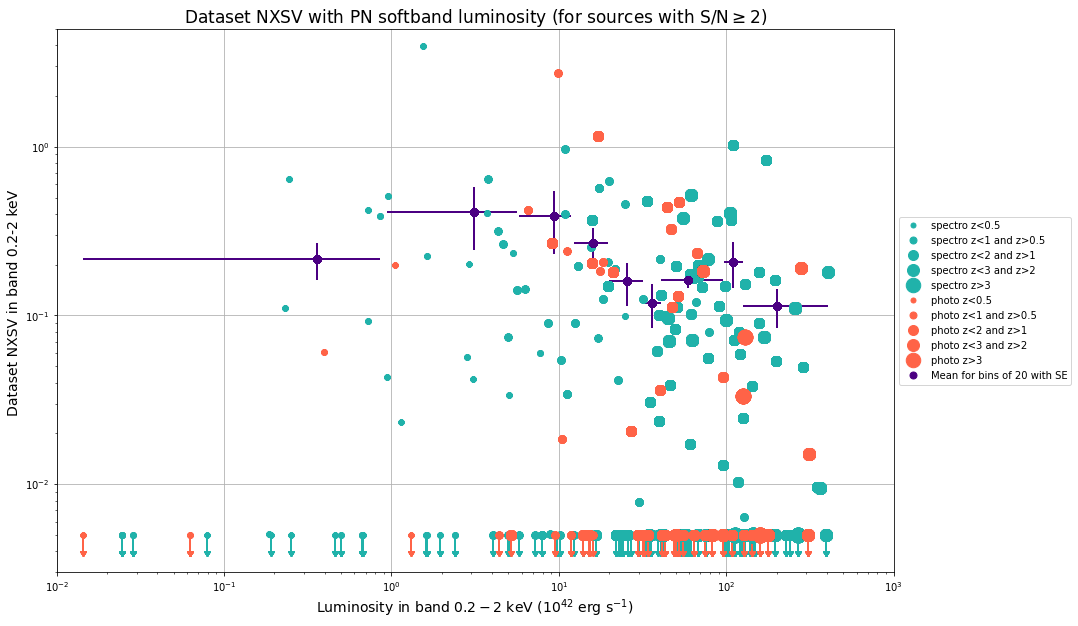
\includegraphics[width=1.12\linewidth]{Figures/NXSVclassic_sn2.png} \caption{ Η \textlatin{NXSV} με λαμπρότητα και \textlatin{binning} κατά λαμπρότητα σε \textlatin{bin} των 20 τουλάχιστον πηγών με διαφοροποίηση για \textlatin{redshift} και επιλέγοντας πηγές με \textlatin{S/N}$>2$. Η λαμπρότητα είναι προσαρμοσμένη στο σύστημα ηρεμίας της πηγής και σημειώνεται στον οριζόντιο λογαριθμικό άξονα σε κλίμακα $10^{42}$ \textlatin{erg s}$^{-1}$ για την παρατηρούμενη ενεργειακή μπάντα $0.2-2$ \textlatin{keV}. Η \textlatin{NXSV} είναι αδιάστατο μέγεθος και σημειώνεται στον κατακόρυφο λογαριθμικό άξονα για την παρατηρούμενη ενεργειακή μπάντα $0.2-2$ \textlatin{keV}.} \label{fig:NXSV_classic_sn2}
    \end{figure*}

 \begin{figure*}  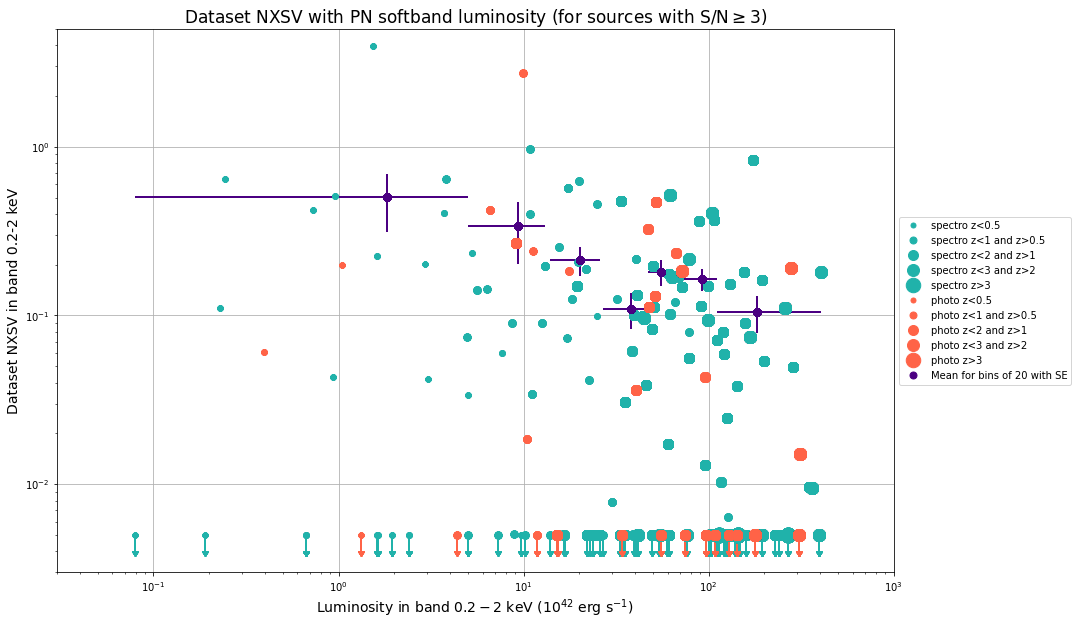
\includegraphics[width=1.12\linewidth]{Figures/NXSVclassic_sn3.png} \caption{ Η \textlatin{NXSV} με λαμπρότητα και \textlatin{binning} κατά λαμπρότητα σε \textlatin{bin} των 20 τουλάχιστον πηγών με διαφοροποίηση για \textlatin{redshift} και επιλέγοντας πηγές με \textlatin{S/N}$>3$. Η λαμπρότητα είναι προσαρμοσμένη στο σύστημα ηρεμίας της πηγής και σημειώνεται στον οριζόντιο λογαριθμικό άξονα σε κλίμακα $10^{42}$ \textlatin{erg s}$^{-1}$ για την παρατηρούμενη ενεργειακή μπάντα $0.2-2$ \textlatin{keV}. Η \textlatin{NXSV} είναι αδιάστατο μέγεθος και σημειώνεται στον κατακόρυφο λογαριθμικό άξονα για την παρατηρούμενη ενεργειακή μπάντα $0.2-2$ \textlatin{keV}.}  \label{fig:NXSV_classic_sn3}
   \end{figure*}

 \begin{figure*}  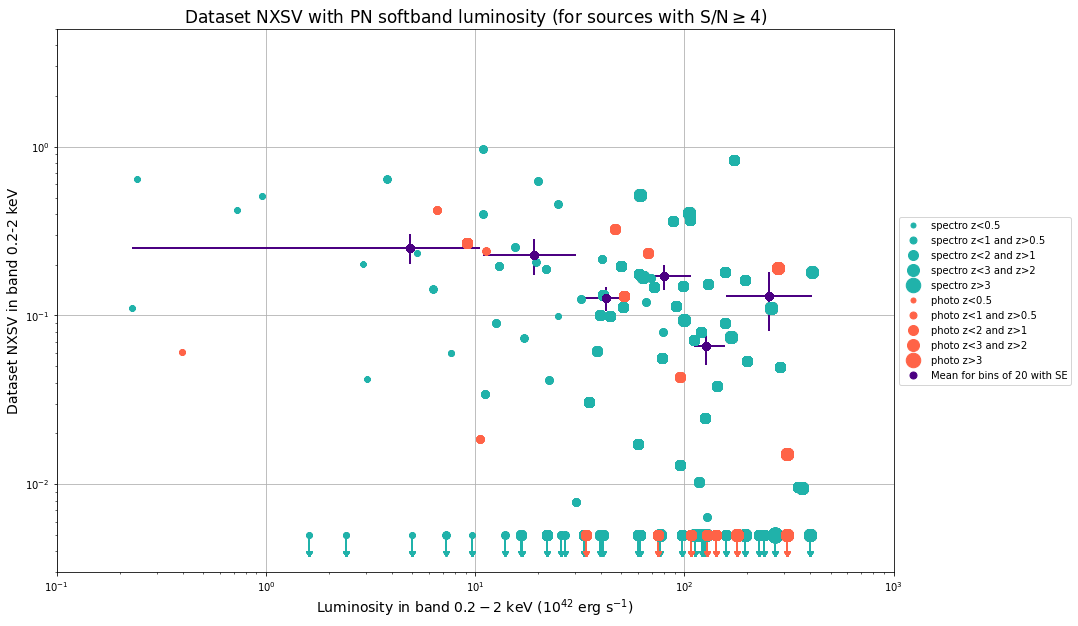
\includegraphics[width=1.12\linewidth]{Figures/NXSVclassic_sn4.png} \caption{ Η \textlatin{NXSV} με λαμπρότητα και \textlatin{binning} κατά λαμπρότητα σε \textlatin{bin} των 20 τουλάχιστον πηγών με διαφοροποίηση για \textlatin{redshift} και επιλέγοντας πηγές με \textlatin{S/N}$>4$. Η λαμπρότητα είναι προσαρμοσμένη στο σύστημα ηρεμίας της πηγής και σημειώνεται στον οριζόντιο λογαριθμικό άξονα σε κλίμακα $10^{42}$ \textlatin{erg  s}$^{-1}$ για την παρατηρούμενη ενεργειακή μπάντα $0.2-2$ \textlatin{keV}. Η \textlatin{NXSV} είναι αδιάστατο μέγεθος και σημειώνεται στον κατακόρυφο λογαριθμικό άξονα για την παρατηρούμενη ενεργειακή μπάντα $0.2-2$ \textlatin{keV}.} \label{fig:NXSV_classic_sn4}
  \end{figure*}
 
Στα σχήματα (\ref{fig:NXSV_classic_sn2}, \ref{fig:NXSV_classic_sn3}, \ref{fig:NXSV_classic_sn4}) βλέπουμε την κατανομή της \textlatin{NXSV} όπως την υπολογίσαμε για κάθε πηγή σύμφωνα με τον τύπο (\ref{eq:NXSV}) με την λαμπρότητα στο αδρανειακό σύστημα ηρεμίας που καταγράφουμε  στις μαλακές ακτίνες Χ ($0.2-2$ \textlatin{keV}) σύμφωνα με τις σχέσεις (\ref{eq:LumiFluxRest},\ref{eq:DL}, \ref{eq:Dcmr})- η οποία υπολογίστηκε από φασματοσκοπικές μετρήσεις \textlatin{redshift} για κάθε πηγή, ή φωτομετρικό για τις πηγές που δεν διέθεταν φασματοσκοπικό. Οι πηγές για τις οποίες υπολογίσαμε τιμή τιμή \textlatin{NXSV} μικρότερη από $0.005$ εμφανίζονται στο επίπεδο $0.005$ του γραφήματος για λόγους εξοικονόμησης χώρου. \\
Επίσης, έχουμε ομαδοποιήσει (\textlatin{binning}) τις πηγές αρχίζοντας από τις χαμηλότερες λαμπρότητες και φτιάχνοντας ομάδες (\textlatin{bin}) των 20 πηγών με σκοπό να αναπαραστήσουμε την μέση τιμή του κάθε \textlatin{bin} ώστε να φανεί η συσχέτιση της \textlatin{ensemble NXSV} με την λαμπρότητα πιο καθαρά (έχει επισημαθεί ότι η \textlatin{ensemble NXSV} δείνει χρήσιμα αποτελέσματα για συλλογή τουλάχιστον 20 καμπύλων φωτός \cite{2013ApJ...771....9A}). Ορισμένες ομάδες (οι δύο ομάδες με τις υψηλότερες λαμπρότητες για \textlatin{S/N}$>2$, και η μια ομάδα με την υψηλότερη λαμπρότητα για \textlatin{S/N}$>3$) περιέχουν περισσότερες από 20 πηγές. Στον υπολογισμό της μέσης τιμής \textlatin{NXSV}, δηλαδή της \textlatin{ensemble NXSV} για κάθε ομάδα, έχουμε υπολογίσει τον καθαρό αριθμητικό μέσο της \textlatin{NXSV} κάθε πηγής. Στον υπολογισμό αυτόν δεν αποκλείσαμε πηγές με μηδενική ή αρνητική τιμή $\sigma_{rms}^2$, διότι τότε θα εισαγάγαμε  μεροληψία \textlatin{(bias)} στο δείγμα\cite{2017MNRAS.471.4398P}\cite{2013ApJ...771....9A}. Η μέση τιμή αυτή είναι η \textlatin{ensemble NXSV} για κάθε ομάδα πηγών και εκτιμά καλώς\cite{2017MNRAS.471.4398P}\cite{2013ApJ...771....9A} την εγγενή μεταβλητότητα όλων των πηγών (δεδομένου ότι όλες οι πηγές σε κάθε \textlatin{bin} λαμπρότητας έχουν παρόμοιες ιδιότητες και χαρακτηριστικά). \\
Οι σημάνσεις σφαλμάτων έγιναν ως εξής: το σφάλμα στις λαμπρότητες εκτείνεται από την χαμηλοτερη εως υψηλότερη τιμή λαμπρότητας των πηγών που περιέχονται στο \textlatin{bin} (είναι δηλαδή το πλάτος του \textlatin{bin}), το σφάλμα στην \textlatin{NXSV} του κάθε \textlatin{bin} είναι σφάλμα μέσης τιμής \textlatin{(standard errror)}. Για κάθε \textlatin{bin} των 20 (ή παραπάνω) πηγών:
$$ \overline{\sigma_{rms}}_{,err}  =\dfrac{ \sqrt{ \sum_{j=1}^{20}(\sigma_{rms, j}- \overline{\sigma_{rms}})^2}}{(20-1)(20)}$$

Εξετάζοντας τα σχήματα (\ref{fig:NXSV_classic_sn2}, \ref{fig:NXSV_classic_sn3}, \ref{fig:NXSV_classic_sn4}), παρατηρούμε αντισυσχέτιση (\textlatin{anticorrelation}) των μεγεθών αυτών, το οποίο είναι συνεπές με αντίστοιχες έρευνες \textlatin{AGN} που έχουν παρουσιαστεί σε εργασίες πάνω σε διαφορετικά πεδία (π.χ. \textlatin{CDF-S}) και διαφορετικές χρονικές κλίμακες \cite{2017MNRAS.471.4398P}. 

Προκειμένου να ελατώσουμε τον θόρυβο στο δείγμα, αλλά και να έχουμε αρκετές πηγές ώστε να δουλέψουμε, επιλέγουμε από εδώ κι έπειτα να χρησιμοποιήσουμε τον περιορισμό \textlatin{S/N}$>3$ για τον λόγο σήματος προς θόρυβο του δείγματός μας, αυτό περιορίζει δραστικά το δείγμα μας σε 175 πηγές.

Έτσι για \textlatin{S/N}$>3$, με αρχική υπόθεση ($P_{null}$) ότι δεν υπάρχει συσχέτιση μεταξύ της κλασσικά υπολογισμένης \textlatin{NXSV} $\sigma_{rms}^2$ και του λογαρίθμου της λαμπρότητας σε μαλακές ακτίνες Χ $\log L_X$, για το στατιστικό τεστ \textlatin{Kendall's} $\tau$ ο συντελεστής συσχέτισης $\sigma_{rms}^2$ και $\log L_X$ για τις πηγές με φασματοσκοπικό $z$ είναι $\tau_{spectro} =-0.092$ ενώ για τις πηγές με φωτομετρικό $z$ είναι $\tau_{photo} = -0.141$ τα οποία αντιστοιχούν σε $P_{null, spectro} = 0.101$ kai $P_{null, photo} = 0.266$. Τα αρνητικά πρόσημα στους συντελεστές υποδηλώνουν φθίνουσα μονότονη σχέση, ενώ θεωρούμε ότι υπάρχει (αντι)συσχέτιση αν έχουμε τιμή σημαντικότητας $P_{null}<5\%$, το οποίο δεν ισχύει ούτε για τις πηγές με φασματοσκοπικό ούτε και για τις πηγές με φωτομετρικό $z$.
Σε πλήρη αναλογία, το στατιστικό τεστ \textlatin{Spearman's rank} δίνει συντελεστή συσχέτισης $\rho_{spectro} =-0.134$ me $P_{null, spectro} = 0.110>0.05$ για τις πηγές με φασματοσκοπικό \textlatin{redshift} kai $\rho_{photo} = -0.211$ me $P_{null, photo} =0.246>0.05$ για τις πηγές με φωτομετρικό \textlatin{redshift}- δηλαδή επιβεβαιώνεται η μη συσχέτιση της $\sigma_{rms}^2$ των πηγών με την λογαριθμική λαμπρότητα $\log L_X$. \\
Για το σύνολο των πηγών (ανεξαρτήτως διαχωρισμού \textlatin{redshift}), το τεστ \textlatin{Kendall's} $\tau$ δίνει συντελεστή συσχέτισης $\tau_{tot} = -0.098$ me $P_{null, tot}= 0.053 $ (οριακά $>0.05$) ενώ το τεστ \textlatin{Spearman's rank} δίνει συντελεστή συσχέτισης $\rho_{tot} = -0.145$ me $P_{null, tot} = 0.055$ (οριακά $>0.05$), οπότε και στο σύνολο των πηγών δεν επιβεβαιώνεται η αντισυσχέτιση σε επίπεδο σημαντικότητας $95\%$\footnote{Η διεξαγωγή των στατιστικών ελέγχων έγινε με τις μεθόδους \textlatin{scipy.stats.kendalltau} kai \textlatin{scipy.stats.spearmanr} της βιβλιοθήκης \textlatin{SciPy.}}, (όμως επιβεβαιώνεται σε επίπεδο σημαντικότητας $90\%$). \\
Για την \textlatin{ensemble NXSV} ο έλεγχος \textlatin{Kendall's} $\tau$ δίνει συντελεστή συσχέτισης $\tau = -0.810$ και ο έλεγχος \textlatin{Spearman's rank} δίνει συντελεστή συσχέτισης $\rho= -0.893$ me τιμές σημαντικότητας $P_{null, \tau} =0.011<0.05$ kai $P_{null, \rho} = 0.007<0.05$ αντίστοιχα. Έχουμε δηλαδή ισχυρή ένδειξη αντισυσχέτισης της \textlatin{ensemble NXSV} με την λογαριθμική λαμπρότητα.\\ 
Προσαρμόζουμε γραμμική σχέση μέσω γραμμικής παλινδρόμησης (\textlatin{linear regression}) sta δεδομένα και βρίσκουμε κλίση $-0.11$ (δηλαδή $\sigma_{rms}^2\propto L_X^{-0.11}$) με σφάλμα μέσης τιμής $StErr = 0.04 $ για τις όλες τις πηγές μαζί. Επαναλαμβάνουμε για την \textlatin{ensemble NXSV} και βρίσκουμε και πάλι κλίση $-0.11$ (δηλαδή $\sigma_{rms, ensemble}^2= \overline{\sigma_{rms}^2}\propto L_X^{-0.11}$) με σφάλμα μέσης τιμής $StErr = 0.01 $, έτσι επιβεβαιώνεται η αντισυσχέτιση \footnote{Η γραμμική παλινδρόμηση έγινε με την μέθοδο \textlatin{scipy.stats.linregress} της βιβλιοθήκης \textlatin{SciPy.}}.

Το συμπέρασμα της αντισυσχέτισης του πλάτους μεταβλητότητας $\sigma_{rms, ensemble}^2$ με την λογαριθμική λαμπρότητα $\log L_X$ στις ενέργειες $0.2-2$ \textlatin{keV}, στο οποίο καταλήγουμε λαμβάνοντας υπ> όψιν τις τιμές μόνο (χωρίς να συνυπολογίζουμε σφάλματα) μας υποδεικνύει πως οι \textlatin{AGN} με μεγαλύτερη λαμπρότητα είναι λιγότερο μεταβλητοί.\\
Αντισυσχέτιση πλάτους μεταβλητότητας \textlatin{AGN} με λαμπρότητα σημαίνει πώς οι λαμπρότεροι \textlatin{AGN} είναι λιγότερο μεταβλητοί, το οποίο από την σχέση \textlatin{Eddington} συνεπάγεται πως οι \textlatin{AGN} με την μεγαλύτερη μάζα μελανής οπής είναι οι λιγότερο μεταβλητοί. Αν δεχτούμε ότι η κύρια αιτία μεταβλητότητας είναι αστάθειες στον δίσκο προσάυξησης, τότε η αντισυσχέτιση θα υποδείκνυε ότι οι \textlatin{AGN} με τις μεγαλύτερες μάζες μελανής οπής είναι αυτοί με τις λιγότερες αστάθειες στην διαδικασία προσαύξησης.\\
Παρ> όλα αυτά, η μεγάλη αβεβαιότητα μας εμποδίζει να βγάλουμε οριστικό συμπέρασμα για την (αντι)συσχέτιση ή μη του πλάτους μεταβλητότητας με την λαμπρότητα στο ενεργειακό παράθυρο $0.2-2$ \textlatin{keV}. 


%{\color{red} AGE: (Ερμηνεια αντισυσχέτισης συντομα εδω και στη συνεχεια στη συζητηση!!!!!). }
 % Platform
	
	\chapter{Αλγόριθμος \textlatin{Bayes} } \label{experimentationANDresults}

\section{Θεμελιώδης στατιστική \textlatin{Bayes}} 
%-Bayesian foundation and implementation [Loredo 2004, Feroz & Hobson 2008]
Προκειμένου να καταλήξουμε σε ένα συμπέρασμα υπολογίζουμε πιθανότητες της υπόθεσης που μας ενδιαφέρει- η οποία ποσοτικοποιείται σε ένα σετ παραμέτρων $\Theta$- έχοντας διαθέσιμα δεδομένα $D$ και έχοντας υποκείμενες εικασίες- δηλαδή ένα μοντέλο $Μ$. Το θεώρημα \textlatin{Bayes} εκφράζει την εκ των υστέρων αυτή πιθανότητα (\textlatin{posterior probability})\cite{Loredo}: 
\begin{equation}\begin{aligned} p (\Theta |D,M)= \dfrac{ p (\Theta |M) \cdot p (D |\Theta ,M) }{ p (D|M)}  \label{eq:BayesTheorem}\end{aligned}\end{equation}
Όπου:\\
-$p (\Theta |D,M)$ : η εκ των υστέρων κατανομή πιθανότητας για τις παραμέτρους $\Theta$ (\textlatin{posterior probability}- στο εξής θα αναφερόμαστε σε αυτήν ως \textlatin{posterior}).\\
-$p (\Theta |M)$ : η εκ των προτέρων κατανομή πιθανότητας για τις παραμέτρους $\Theta$ (\textlatin{prior probability}- στο εξής θα αναφερόμαστε σε αυτήν ως \textlatin{prior}).\\
-$p (D |\Theta ,M)$ : η δειγματοληπτική κατανομή των δεδομένων $D$ δηλαδή το ενδεχόμενο να παρατηρήσουμε τα δεδομένα $D$ θεωρώντας μοντέλο $Μ$ με παραμέτρους $\Theta$ (\textlatin{likelihood}- στο εξής θα αναφερόμαστε σε αυτήν ως \textlatin{likelihood}).\\
-$p (D|M)$ : η <<προγνωστική>> κατανομή δεδομένων, $Ζ$ (\textlatin{evidence}- στο εξής θα αναφερόμαστε σε αυτήν ως \textlatin{evidence}).

Στην συμπερασματολογία (εκτίμηση παραμέτρων) ενδιαφερόμαστε για το πώς η \textlatin{posterior} $p (\Theta |D,M)$ μεταβάλεται με τις παραμέτρους $\Theta$ όταν τα δεδομένα $D$ έχουν σταθερές τιμές. Οπότε, μεγαλύτερη σημασία έχει το πώς η δειγματοληπτική κατανομή $p (D |\Theta ,M)$ μεταβάλεται με τις μαραμέτρους $\Theta$, και όχι μετα δεδομένα $D$, γι> αυτό την ονομάζουμε ενδεχόμενο για τις $\Theta$ (\textlatin{likelihood}) $\mathcal{L}\equiv p (D |\Theta ,M)$. Η \textlatin{evidence} $p (D|M)$ δεν έχει εξάρτηση από τις παραμέτρους $\Theta$ έτσι, λοιπόν, έχει τον ρόλο κανονικοποιητικού παράγοντα για την $\textlatin{posterior}$ που υπολογίζεται ως τέτοιος: \begin{equation}\begin{aligned} p (D|M) = \int_{\Omega_\Theta}  p (D |\Theta ,M)\cdot p (\Theta |M)   d\Theta \label{eq:evidence}\end{aligned}\end{equation}
Η \textlatin{posterior} $p (\Theta |D,M)$ συνιστά την πλήρη συμπερασματολογία \textlatin{Bayes} για τις τιμές των παραμέτρων και μπορεί να ολοκληρωθεί για κάθε παράμετρο. Αν χωρίσουμε τις $\Theta$ σε παραμέτρους που μας ενδιαφέρουν $\psi$ και αδιάφορες παραμέτρους $\phi$, τότε η συμπερασματολογία για τις $\psi$ είναι η ολοκληρωμένη κατανομή που προκύπτει ολοκληρώνοντας την \textlatin{posterior} ως προς τις παραμέτρους $\phi$\cite{Loredo}:
\begin{equation}\begin{aligned} p (\psi |D,M)=\int_{\Omega_\phi} p (\Theta |D,M) d\phi = \int_{\Omega_\phi} p (\psi , \phi |D,M) d\phi \label{eq:MarginalDistri}\end{aligned}\end{equation}
To θεώρημα \textlatin{Bayes} εφαρμόζεται τόσο για υπολογισμό \textlatin{posterior} κατανομών πυκνότητας πιθανότητας όσο και για διακριτές \textlatin{posterior} κατανομές πιθανότητας, όπου αντί για ολοκληρώματα έχουμε αθροίσματα.

\subsection{Τεχνικές δειγματοληψίας \textlatin{Markov Chain Monte Carlo (MCMC)}}

Ο αλγόριθμος δειγματοληψίας \textlatin{Markov Chain Monte Carlo (MCMC)} είναι μια μέθοδος \textlatin{Bayes} που χρησιμοποιείται για ολοκλήρωση και εκτίμηση παραμέτρων. Ο αλγόριθμος σε κάθε βήμα συγκρίνει ένα αρχικό σημείο με ένα τυχόν σημείο από μία αρχική κατανομή με τοπική μεροληψία. Με πιθανότητα ανάλογη του πηλίκου των δύο σημείων ο αλγόριθμος επιλέγει ένα νέο σημείο ως σημείο εκκίνησης του επόμενου βήματος. Με κάθε επανάληψη παράγεται ένα σημείο, οπότε δημιουργείται μία αλυσίδα που έχει την ιδιότητα να αναπαριστά τα ανύσματα παραμέτρων $\Theta$ σε αναλογία με την πιθανότητά τους. Αυτή η αναπαράσταση του παραμετρικού χώρου μπορεί να ολοκληρωθεί ως προς τις παραμέτρους που δεν μας ενδιαφέρουν για να εξετάσουμε την κατανομή των παραμέτρων που μας ενδιαφέρουν.  
Η διάδοση σφαλμάτων στις εξαγόμενες ποσότητες μπορεί να γίνει σχολαστικά χωρίς να υιοθετήσουμε σφάλματα κατανομής \textlatin{Gauss}\cite{BuchnerGeorgakakis}.
H συμπερασματολογία ακολουθώντας τεχνικές \textlatin{Markov Chain Monte Carlo (MCMC)} γίνεται με δείγματα από μη-κανονικοποιημένη \textlatin{posterior} με αποτέλεσμα στην ισορροπία να έχουμε μια αλυσίδα που περιέχει ένα δείγμα του παραμετρικού χώρου κατανεμειμένο σύμφωνα με την \textlatin{posterior} με μετρική που υπαγορεύει η \textlatin{prior} χωρίς όμως να είναι κανονικοποιημένη. 

\subsection{Αλγόριθμος ένθετης δειγματοληψίας \textlatin{Nested Sampling (NS)}}

Η συμπερασματολογία \textlatin{Bayes} ενέχει δύο υπολογιστικές προκλήσεις. Πρώτον, κατά την εκτίμηση των παραμέτρων $\Theta$ ενός μοντέλου $Μ$ για τα δεδομένα $D$ η \textlatin{posterior} κατανομή μπορεί να είναι πολυτροπική \textlatin{(multi-modal)}- τότε η σύγκλιση σε στατική κατάσταση (ισορροπία) της παραδοσιακής τεχνικής \textlatin{MCMC} γίνεται πολύ αργή. Δεύτερον, κατά την επιλογή μοντέλου, η κατανομή \textlatin{evidence} (σχέση \ref{eq:evidence}) ως κανονικοποιητικός παράγοντας πρέπει να υπολογιστεί- αυτό σημαίνει υπολογισμό πολυδιάστατων ολοκληρωμάτων στον παραμετρικό χώρο, όταν η μετρική του παραμετρικού χώρου δίνεται από την \textlatin{prior}.\\
Η τεχνική της ένθετης δειγματοληψίας \textlatin{(Nested Sampling, NS)} είναι μια σύγχρονη τεχνική \textlatin{Monte Carlo} που εστιάζει στον υπολογισμό του ολοκληρώματος αυτού και επιτρέπει τον υπολογισμο της \textlatin{posterior} κατορθώνοντας ταυτόχρονα και εκτίμηση παραμέτρων και επιλογή μοντέλου\cite{Feroz2019}.
Προτέρημα του αλγορίθμου \textlatin{nested sampling}, εκτός από τον υπολογισμό πολυδιάστατων ολοκληρωμάτων, είναι ο εύκολος χειρισμός συναρτήσεων δειγματοληπτικής κατανομής (\textlatin{likelihood}) που μπορεί να είναι πολυτροπικές ή με περίεργο σχήμα. Ο αλγόριθμος \textlatin{NS} εκτιμά ολοκληρώματα εντοπίζοντας πώς τμήμα του όγκου παραμετρικού χώρου (όγκο τον οποίο υπαγορεύει η \textlatin{prior}) συρρικνώνεται όταν σταδιακά αυξάνουμε το όριο της \textlatin{likelihood}. Η μείωση στην επιφάνεια (για \textlatin{prior} που ορίζει επιφάνεια παραμετρικού χώρου) σε ένα βήμα πολλαπλασιασμένη με το ύψος του βήματος στην \textlatin{likelihood} προσεγγίζει τον συνολικό όγκο αθροίζοντας, ανεξαρτήτως του σχήματος της επιφάνειας που αντιστοιχεί στο βήμα. Στην διαδικασία αυτή παράγει την \textlatin{posterior} πιθανότητα για τις παραμέτρους και υπολογίζει το ολοκλήρωμα στον παραμετρικό χώρο\cite{Buchner2014}. 
%Nested Sampling (NS, Skilling, 2004) is a Monte Carlo algorithm for com-puting the integral over a model parameter space. In the context of Bayesian inference, theintegrand is the likelihood function, which is marginalised over the parameter space accord-ing to the prior definition (which donates the space metric). The integralZis known as themarginal likelihood or Bayesian evidence. \cite{Buchner2021}

%%------------------------------------------%%

\section{Εφαρμογή συμπερασματολογίας \textlatin{Bayes} στον αλγόριθμο υπολογισμού της \textlatin{NXSV}}

%{\color{red} στον αλγοριθμο υπολογισμου της excess variance?}

Σε κάθε πηγή \textlatin{AGN} που μελετάμε αντιστοιχεί μια καμπύλη φωτός, κάθε σημείο της καμπύλης φωτός είναι μία παρατήρηση με καταγεγραμμένη διάρκεια και καταγεγραμμένο αριθμό φωτονίων σε δεδομένη ενέργεια και ανιχνευτικό μέσο.

Τα δεδομένα μας ($D$) είναι οι καταμετρήσεις φωτονίων για κάθε παρατήρηση (καταμετρήσεις φωτονίων για κάθε σημείο της καμπύλης φωτός) μιας πηγής.\\
%({\color{red} στοχαστικη διαδικασια δεν σημαινει αναγκαστικα νορμαλ, απλα οτι υπαρχει μη περιοδικη μεταβλητοτητα. Η υποθεση οτι οι μεταβολες ακολοθουν την κατανομη νορμαλ ειναι προσθετη υποθση}) 
Το μοντέλο ($Μ$) που ακολουθούμε είναι η υπόθεση ότι η παραγωγή φωτονίων ακτίνων Χ από εναν \textlatin{AGN} είναι μία στοχαστική διαδικασία που διέπεται από στατιστική \textlatin{Gauss}. Οπότε η υπόθεσή μας είναι ότι ο ρυθμός καταμέτρησης φωτονίων μίας πηγής ($CR$) έχει έναν πραγματικό μέσο $CR_{mean}$ και εγγενή διακύμανση $\sigma_{intr}$ η οποία είναι η μη-κανονικοποιημένη πραγματική διακύμανση \begin{equation}
\sigma_{rms}^2 = \frac {\sigma_{intr}^2}{CR_{mean}^2} \iff  \sigma_{intr} = \sqrt{\sigma_{rms}^2 \cdot CR_{mean}^2} \label{eq:SigmaIntr}\end{equation}
Επίσης στο μοντέλο $Μ$ λαμβάνουμε υπ> όψιν ότι η καταγραφή φωτονίων δεν είναι απλώς τα φωτόνια του στοχαστικού σήματος κανονικής κατανομής, αλλά περιέχεται θόρυβος που διέπεται από στατιστική \textlatin{Poisson}. Την υπόθεση αυτή βασίζουμε στο γεγονός ότι η καταγραφή φωτονίων από ανιχνευτή ακτίνων Χ ακολουθεί κατανομή \textlatin{Poisson} με αναμενόμενη τιμή που εξαρτάται από την ροή της πηγής. Έπειτα έχουμε ήδη εκφράσει την υπόθεση ότι αναμένουμε η καταγραφή φωτονίων στον ανιχνευτή για μία παρατήρηση να είναι $ CR \cdot t_{exp}\cdot \mbox{\textlatin{EEF}} + B$, όπου $ CR \cdot t_{exp}\cdot \mbox{\textlatin{EEF}}$ είναι η απόκριση του ανιχνευτή μας στον ρυθμό φωτονίων $CR$ της πηγής και $Β$ το υπόβαθρο.\\
%{\color{red} Ισως αξιζει να τονιστει οτι η καταγραφη φωτονιων απο ενα ανιχνευτη-Χ ακολουθει την κατανομη \textlatin{Poisson}, με αναμενομη τιμη που εξαρταται απο τη ροη τησ πηγης.?}
Οι παράμετροι ($\Theta$) του μοντέλου μας επιλέγουμε να είναι oi $(CR_{mean}, \sigma_{rms}^2)$.
Σκοπός μας είναι να κατασκευάσουμε έναν αλγόριθμο που εκτιμά τις παραμέτρους μας $(CR_{mean}, \sigma_{rms}^2)$, δηλαδή για κάθε πηγή του δείγματός μας να εκτιμήσουμε βάσει του αλγορίθμου τον μέσο ρυθμό φωτονίων και την  \textlatin{NXSV.} 

\subsection{Υπολογισμός ενδεχομένου παρατήρησης των φωτονίων για μία πηγή, μία καμπύλη φωτός}

\subsubsection*{Διαδικασία \textlatin{Poisson}: πιθανότητα να παρατηρήσουμε $Ν$ φωτόνια στην καμπύλη φωτός}

Τα δεδομένα μας (καταμετρήσεις φωτονίων) είναι σε διακριτά διαστήματα και οι καταμετρήσεις είναι ανεξάρτητες μεταξύ τους. Σχηματικά, μπορούμε να διαιρέσουμε νοητά τον χώρο δεδομένων σε \textlatin{bin} χρονικού διαστήματος παρατήρησης. Αν υποθέσουμε ότι σε ένα ορισμένο μοντέλο $M$ αναμένουμε να υπάρχουν $\lambda_i$ προσμετρήσεις φωτονίων στο \textlatin{bin} $i$, τότε- αν το μοντέλο είναι σωστό- η πιθανότητα να παρατηρήσουμε ακριβώς $N_i$ φωτόνια στο \textlatin{bin} $i$ των δεδομένων μας βρίσκεται από την κατανομή \textlatin{Poisson}: 
\begin{equation}\begin{aligned} \mathcal{P}(N|\lambda) =  \prod_{i=1}^{N_{obs}} \mathcal{P}_i(N_i|\lambda_i)   = \prod_{i=1}^{N_{obs}} \dfrac{{\lambda_i}^{N_i}}{N_i !} e^{-\lambda_i}   \label{eq:Poisson_i}\end{aligned}\end{equation}
Όπου:\\
- $ \lambda_i$ : η αναμενόμενη τιμή \textlatin{Poisson} για το \textlatin{bin} $i$. \\ 
- $N_i$ : το πλήθος καταμετρήσεων φωτονίων μαλακών ακτίνων Χ για το \textlatin{bin} $i$/ για το $i-$οστό σημείο της καμπύλης φωτός.\\
- $N_{obs}$ : το πλήθος των \textlatin{bin} $i$/ διαστήματα παρατηρήσεων, δηλαδή το πλήθος των σημείων στην καμπύλη φωτός.\\ 
- Ο παράγοντας $\prod_{i=1}^{N_{obs}} \frac{1}{ N_i !}$ είναι ανεξάρτητος του μοντέλου (εξαρτάται μόνο από τα δεδομένα).  

\subsubsection*{Στοχαστική διαδικασία \textlatin{Gauss}: πιθανότητα να παρατηρήσουμε δεδομένο  \textlatin{CR} στην καμπύλη φωτός}

Θα θεωρήσουμε στατιστική \textlatin{Gauss}, δηλαδή ότι ο ρυθμός φωτονίων του στοχαστικού σήματος της πηγής ακολουθεί κανονική κατανομή $CR \sim \mathcal{N} (CR_{mean}, \sigma_{intr}^2)$ gia καμπύλη φωτός με μέση τιμή $CR_{mean} = \frac{1}{N_{obs}} \sum_{i=1}^{N_{obs}} CR_i$ και εγγενή διακύμανση $\sigma_{intr}^2$. Η (υλοποιημένη) συνάρτηση πυκνότητας πιθανότητας να έχουμε τις $N_{obs}$ το πλήθος τιμές $CR_i$ που έχουμε στα δεδομένα μας υπολογίζεται:  
\begin{equation}\begin{aligned} {p} (CR|\sigma_{intr})= {} & \prod_{i=1}^{N_{obs}} \mathcal{N}_i(CR_i| \sigma_{intr}) =\\ & = \prod_{i=1}^{N_{obs}} \dfrac{exp \big(-\frac{1}{2} \frac{( CR_i-CR_{mean} )^2}{\sigma_{intr}^2}  \big)} {\sqrt{2\pi} \cdot \sigma_{intr}}  \label{eq:Gauss_tot}\end{aligned}\end{equation}
Όπου:\\
- $CR_i$ : ο ρυθμός καταμέτρησης φωτονίων που καταγράφηκε στο $i-$οστό σημείο της καμπύλης φωτός της πηγής (υλοποιημένη ποσότητα)\\
- $\sigma_{intr}$ : η εγγενής διακύμανση της πηγής.\\
- $ CR_{mean}$ : ο εγγενής μέσος ρυθμός καταμέτρησης φωτονίων της πηγής.

\subsubsection*{Στοχαστική διαδικασία \textlatin{Gauss}: πιθανότητα αναμενόμενης τιμής \textlatin{Poisson} στην καμπύλη φωτός}

Η αναμενόμενη τιμή \textlatin{Poisson} για δεδομένο σημείο καμπύλης φωτός $i$ (δηλαδή με δεδομένο χρόνο έκθεσης $t_i$, κλάσμα της \textlatin{PSF} $EEF_i$ kai υπόβαθρο $B_i$) όπως συζητήθηκε για την σχέση \ref{eq:sourcesignal}:    
$$\lambda_i = CR \cdot t_i \cdot EEF_i + B_i$$ 
Αφού ο \textlatin{CR} ακολουθεί κανονική κατανομή $ CR \sim \mathcal{N} (CR_{mean}\;,\; \sigma_{intr}^2)$, τότε το $\lambda$ θα ακολουθεί κατανομή $\lambda \sim \mathcal{N} (t\cdot \mbox{\textlatin{EEF}} \cdot CR_{mean}+ B\;,\; t^2 \mbox{\textlatin{EEF}}^2\sigma_{intr}^2)$, οπότε η συνάρτηση πυκνότητας πιθανότητας να έχουμε αναμενόμενη τιμή \textlatin{Poisson}  $\lambda$ για όλα τα σημεία της καμπύλης φωτός:
\begin{equation}\begin{aligned} {p} (\lambda|CR, \sigma_{intr})= {} & \prod_{i=1}^{N_{obs}} \mathcal{N}_i(\lambda_i| CR,\sigma_{intr}) = \prod_{i=1}^{N_{obs}} \dfrac{exp \big(-\frac{1}{2} \frac{( \lambda_i-\lambda_{mean} )^2}{t_i^2\; \mbox{\textlatin{EEF}}_i^2\;\sigma_{intr}^2}  \big)} {\sqrt{2\pi}\; t_i\; \mbox{\textlatin{EEF}}_i\;\sigma_{intr}} =\\ & =    \prod_{i=1}^{N_{obs}} \dfrac{exp \big(-\frac{1}{2} \frac{( \lambda_i-\lambda_{mean} )^2}{\sigma_{new, intr}^2}  \big)} {\sqrt{2\pi} \; \sigma_{new, intr}}   \label{eq:Gauss_lambda}\end{aligned}\end{equation}
Όπου:\\
- $\lambda_i = t_i\cdot \mbox{\textlatin{EEF}}_i \cdot CR + B_i$ : για κάθε σημείο της καμπύλης φωτός.\\
- $\lambda_{mean} = \frac{1}{N_{obs}} \sum_{i=1}^{N_{obs}} \lambda_i$ : μέση αναμενόμενη τιμή \textlatin{Poisson} για όλη την καμπύλη φωτός.\\
- $\sigma_{new, intr}^2 = t_i^2\cdot \mbox{\textlatin{EEF}}_i^2 \cdot \sigma_{intr}^2 $ : διακύμανση της αναμενόμενης τιμής \textlatin{Poisson}.\\

\subsubsection*{Ενδεχόμενο υλοποιημένου πλήθους φωτονίων για στοχαστική κανονική καμπύλη φωτός και θόρυβο \textlatin{Poisson}}

Δεδομένης της εξίσωσης \ref{eq:Gauss_lambda}:
$$ {p} (\lambda|CR, \sigma_{intr})=  \prod_{i=1}^{N_{obs}} \dfrac{exp \big(-\frac{1}{2} \frac{( \lambda_i-\lambda_{mean} )^2}{\sigma_{new, intr}^2}  \big)} {\sqrt{2\pi} \; \sigma_{new, intr}}$$ 
Kai της εξίσωσης \ref{eq:Poisson_i}: 
$$\mathcal{P}(N|\lambda) = \prod_{i=1}^{N_{obs}} \mathcal{P}_i(N_i|\lambda_i) =\prod_{i=1}^{N_{obs}} \dfrac{{\lambda_i}^{N_i}}{N_i !} e^{-\lambda_i} $$

Το ενδεχόμενο (\textlatin{likelihood}) να παρατηρήσουμε $N$ το πλήθος καταγεγραμμένα φωτόνια σε $N_{obs}$ το πλήθος σημεία καμπύλης φωτός- δεδομένου ότι ο $CR$ ακολουθεί κατανομή $\mathcal{N}(CR_{mean}, \sigma_{intr})$-  είναι η δεσμευμένη πιθανότητα να παρατηρήσουμε $N$ φωτόνια για συγκεκριμένη τιμή του $\lambda$ αναλογικά με την πιθανότητα να έχουμε αναμενόμενη τιμή $\lambda$ δεδομένης της κατανομής του $CR$ ολοκληρωμένο για όλες τις τιμές του  $\lambda$:

\begin{equation}\begin{aligned} \mathcal{L} (N|CR, \sigma_{intr})= {} &  \int_0^\infty \mathcal{P}(N|\lambda) \cdot  {p} (\lambda|CR, \sigma_{intr}) d\lambda    =\\ & =    \int_0^\infty  \prod_{i=1}^{N_{obs}} \dfrac{{\lambda_i}^{N_i}}{N_i !} e^{-\lambda_i}  \cdot   \dfrac{exp \big(-\frac{1}{2} \frac{( \lambda_i-\lambda_{mean} )^2}{\sigma_{new, intr}^2}  \big)} {\sqrt{2\pi}\; \sigma_{new, intr}}  d\lambda_i =    \\ & =  \prod_{i=1}^{N_{obs}} \int_0^\infty   \dfrac{{\lambda_i}^{N_i}}{N_i !} e^{-\lambda_i}  \cdot   \dfrac{exp \big(-\frac{1}{2} \frac{( \lambda_i-\lambda_{mean} )^2}{\sigma_{new, intr}^2}  \big)} {\sqrt{2\pi} \; \sigma_{new, intr}}  d\lambda_i =    \\ & =  \prod_{i=1}^{N_{obs}} \mathcal{L}_i (N_i|CR_i, \sigma_{intr, i})  \label{eq:Likelihood_tot}\end{aligned}\end{equation}

Οπότε, για το $i-$οστό σημείο καμπύλης φωτός:
\begin{equation}\begin{aligned} \mathcal{L}_i (N_i|CR_i, {\sigma^\prime}_{ intr, i}) = {} &  \int_0^\infty   \dfrac{{\lambda_i}^{N_i}}{N_i !} e^{-\lambda_i}  \cdot   \dfrac{exp \big(-\frac{1}{2} \frac{( \lambda_i-\lambda_{mean} )^2}{{\sigma^\prime}_{ intr, i}^2}  \big)} {\sqrt{2\pi} \; {\sigma^\prime}_{ intr, i}}  d\lambda_i =    \\ & =  \frac{1}{\sqrt{2\pi} \; N_i! \; {\sigma^\prime}_{ intr, i} } \int_0^\infty  {\lambda_i}^{N_i} e^{-\lambda_i} \cdot exp \Big(-\frac{1}{2} \frac{( \lambda_i-\lambda_{mean} )^2}{{\sigma^\prime}_{ intr, i}^2}  \Big) d\lambda_i  \label{eq:Likelihood_i}\end{aligned}\end{equation}

Όπου: ${\sigma^\prime}_{ intr, i} = t_i \cdot \mbox{\textlatin{EEF}}_i \cdot \sigma_{intr} $

%-------------------------------------------%

\subsection{\textlatin{Importance Sampling}}

\textlatin{Importance Sampling} (ή αλλιώς δειγματοληψία σπουδαιότητας) είναι μια γενική τεχνική για τον υπολογισμό των ιδιοτήτων μιας συγκεκριμένης κατανομής η οποία μας δίνει έναν τρόπο υπολογισμού ολοκληρώματος γινομένου μιας κατανομής με μια συνάρτηση ως προς την τυχαία μεταβλητή της κατανομής κάνοντας δειγματοληψία της μεταβλητής αυτής από την κατανομή που ακολουθεί και ολοκληρώνοντας αριθμητικά (αθροίζοντας, δηλαδή) μόνο την συνάρτηση.
Το ενδεχόμενο να παρατηρήσουμε $N_i$ το πλήθος καταγεγραμμένα φωτόνια sto $i-$οστό σημείο της καμπύλης φωτός (εξίσωση \ref{eq:Likelihood_i}):
$$   \mathcal{L}_i (N_i|CR_i, \sigma_{intr})  =  \int_0^\infty  \frac{1}{N_i!} \cdot{\lambda_i}^{N_i} e^{-\lambda_i} \cdot \frac{1}{\sqrt{2\pi} \; {\sigma^\prime}_{ intr, i}} exp \Big(-\frac{1}{2} \frac{( \lambda_1-\lambda_{mean} )^2}{{\sigma^\prime}_{ intr, i}^2}  \Big) d\lambda_i  $$

Όπου: ${\sigma^\prime}_{ intr, i} = t_i \cdot \mbox{\textlatin{EEF}}_i \cdot\sigma_{intr} $.  

Θέλουμε να υπολογίσουμε την τιμή της συνάρτησης:
$${f_i}(\lambda_i)=  \frac{1}{N_i!} \cdot{\lambda_i}^{N_i} e^{-\lambda_i} $$ όπου η μεταβλητή $\lambda_i$ ακολουθεί κατανομή $\lambda_i \sim {q_i} (\lambda_i) = \dfrac{exp \big(-\frac{1}{2} \frac{( \lambda_i-\lambda_{mean} )^2}{{\sigma^\prime}_{ intr, i}^2}  \big)} {\sqrt{2\pi}  \; {\sigma^\prime}_{ intr, i}}$. \\ 
Έχουμε την εξής εκτίμηση $E[f_i(\lambda_i)]$ για την ${f_i}$:

\begin{equation} E[{f_i}(\lambda_i))] = \int {f_i}(\lambda_i) {q_i} (\lambda_i)d\lambda_i \approx \dfrac{1}{N_{large}} \sum_{j=0}^{N_{large}} {f_i}(\lambda_{ij}) \label{eq:ImportanceSampling}\end{equation}

- $ N_{large}$: μήκος του ανίσματος $\lambda_i$ ($j=1,2,3,..., N_{large}$) που συλλέγεται από την κατανομή ${q_i} (\lambda_i)$.\\
- $j$: αριθμεί τα στοιχεία του μονοδιάστατου ανίσματος $\lambda_i$.\\
- $\lambda_{ij}$: $j-$ στοιχείο του χώρου $\lambda_i$ που συλλέγεται από την κατανομή $\dfrac{exp \big(-\frac{1}{2} \frac{( \lambda_i-\lambda_{mean} )^2}{{\sigma^\prime}_{ intr, i}^2}  \big)} {\sqrt{2\pi} {\sigma^\prime}_{ intr, i}}$\\
- ειδικό βάρος = 1\\
- Η διακύμανση της εκτίμησης του \textlatin{importance sampling}:
$ \dfrac{1}{N_{large}} \cdot Var[{f_i}(\lambda_i))] $\\

Η μέθοδος αυτή υπολογισμού ολοκληρωμάτων που περιέχουν κατανομές ελέγξαμε ότι δίνει με μεγάλη ακρίβεια ίδια αποτελέσματα με διαφορετικούς τρόπους αριθμητικής ολοκλήρωσης και κάνει πολύ γρηγορότερο τον αλγόριθμό μας.

%-------------------------------------------%

\subsection{Ο αλγόριθμος ένθετης δειγματοληψίας \textlatin{UltraNest} kai par'ametroi}

Χρησιμοποιούμε το πακέτο \textlatin{UltraNest}\cite{ULTRANEST} για τον αλγόριθμο εκτίμισης παραμέτρων $(CR_{mean}, \sigma_{rms}^2)$ για κάθε μία από τις 210 πηγές με τριών εποχών παρατηρήσεις από τον ανιχνευτή ΡΝ στις μαλακές ακτίνες Χ $0.2-2$ \textlatin{keV} με λόγo σήματος προς θόρυβο \textlatin{S/N}$>3$. \\
To \textlatin{UltraNest} είναι ένα γενικής χρήσης πακέτο συμπερασματολογίας \textlatin{Bayes} που χρησιμοποιείται για εκτίμηση παραμέτρων και σύγκριση μοντέλων. Αφού ορίσουμε το πλήθος των παραμέτρων που μας ενδιαφέρει στο πρόβλημά μας, το \textlatin{UltraNest} συλλέγει τυχαία ένα σετ Ν το πλήθος σημείων από μοναδιαίο υπερκύβο διαστάσεων όσο το πλήθος των παραμέτρων του μοντέλου μας. Μέσω της αντίστροφης συνάρτησης συσσωρευμένης κατανομής της \textlatin{prior} που εμείς ορίζουμε, το σετ σημείων του μοναδιαίου υπερκύβου απεικονίζεται στον φυσικό παραμετρικό χώρο. Υπολογίζεται η  \textlatin{likelihood} $\mathcal{L}$ για κάθε σημείο σύμφωνα με την συνάρτηση ενδεχομένου που εμείς ορίζουμε για το πρόβλημά μας. Σε αυτό το σετ σημείων ο αλγόριθμος ένθετης δειγματοληψίας \textlatin{NS} αντικαθιστά επανειλημμένα το σημείο στο οποίο αντιστοιχεί η χαμηλότερη τιμή της \textlatin{likelihood} μέσω δειγματοληψίας από την \textlatin{prior} με περιορισμούς που θέτει η \textlatin{likelihood (likelihood-constrained prior sampling, LCPS)}. Σε κάθε επανάληψη $i$ (δηλαδή μετά απο κάθε σημείο που απορρίπτουμε) ο χώρος της \textlatin{prior} συρρικνώνεται κατά περίπου $V_{i+1}/V_i= (N−1)/N$, όπου $V_i=1$ ο αρχικός όγκος της \textlatin{prior}. Το σημείο που απορρίπτεται σε κάθε επανάληψη γίνεται δέιγμα της της \textlatin{posterior} me ειδικό βάρος $w_i=\mathcal{L}_i \times V_i$, αποδίδοντας έτσι την κατανομή \textlatin{posterior} και την εκτίμιση της \textlatin{evidence} $Z_i= \sum_{j=1}^i  w_i$. H επαναληπτική αυτή διαδικασία τερματίζεται όταν τα σημεία του τρέχοντος πληθυσμού (που δεν έχουμε απορρίψει) γίνονται ασήμαντα, δηλαδή όταν το ειδικό τους βάρος γίνει πολύ μικρότερο της \textlatin{evidence}:  $w_{τρεχον} = V_i max_{i=1}^N \mathcal{L}_{τρεχον, i} \ll Z_i$ \cite{ULTRANEST}.

Για το πρόβλημά μας, έχουμε 2 το πλήθος παραμέτρους $(CR_{mean}, \sigma_{rms}^2)$.\\
Ως \textlatin{prior} του προβλήματός μας θέτουμε ένα εύλογο εύρος τιμών για κάθε μία από τις παραμέτρους. Οπότε θέτουμε τον μέσο ρυθμό να ακολουθεί συνεχή ομοιόμορφη κατανομή με ελάχιστη τιμή $10^{-6}$ και μέγιστη τιμή $0.3$, $CR_{mean} \sim \mathcal{U}(10^{-6} , 0.3)$ με συνάρτηση συσσωρευμένης κατανομής 
$$ \mbox{\textlatin{CDF}}_{\mathcal{U}} = \begin{cases} 0   \mbox{\quad \quad \quad \quad \quad \quad \quad \quad \quad ,gia \quad } CR_{mean}<10^{-6}   \\ \dfrac{CR_{mean} - 10^{-6}}{0.3-10^{-6}}  \mbox{\quad \quad  ,gia \quad } CR_{mean} \in (10^{-6}, 0.3) \\ 1  \mbox{\quad \quad \quad \quad \quad \quad \quad \quad \quad ,gia \quad} CR_{mean}>0.3  \end{cases}$$ 
kai αντίστροφη συνάρτηση συσσωρευμένης κατανομής
$$  \mbox{\textlatin{invCDF}}_{\mathcal{U}} = \dfrac{0.3 - CR_{mean}}{0.3-10^{-6}} \mbox{\quad \quad  ,gia \quad } CR_{mean} \in (10^{-6}, 0.3)$$
Ομοίως η εγγενής πραγματική διακύμανση θα ακολουθεί συνεχή ομοιόμορφη κατανομή με ελάχιστη τιμή $10^{-6}$ και μέγιστη τιμή $15$, $\sigma_{rms}^2  \sim \mathcal{U}(10^{-6} , 15)$ με συνάρτηση συσσωρευμένης κατανομής 
$$ \mbox{\textlatin{CDF}}_{\mathcal{U}} = \begin{cases} 0   \mbox{\quad \quad \quad \quad \quad \quad \quad ,gia \quad } \sigma_{rms}^2<10^{-6}   \\ \dfrac{\sigma_{rms}^2 - 10^{-6}}{15-10^{-6}}  \mbox{\quad \quad  ,gia \quad } \sigma_{rms}^2 \in (10^{-6}, 15) \\ 1  \mbox{\quad \quad \quad \quad \quad \quad \quad  ,gia \quad} \sigma_{rms}^2>15  \end{cases}$$ 
kai αντίστροφη συνάρτηση συσσωρευμένης κατανομής
$$  \mbox{\textlatin{invCDF}}_{\mathcal{U}} = \dfrac{0.3 -\sigma_{rms}^2}{15-10^{-6}} \mbox{\quad \quad  ,gia \quad } \sigma_{rms}^2 \in (10^{-6}, 15)$$
Και για τις δύο παραπάνω ποσότητες χρησιμοποιήσαμε την τιμή $10^{-6}$ ως κάτω όριο αντί για την τιμή $0$. Αυτό έγινε επειδή δουλεύουμε σε λογαριθμικό χώρο και η πολύ μικρή ποσότητα $10^{-6}$ θεωρούμε ότι είναι αντιπροσωπευτική του φυσικού κάτω ορίου $0$ χωρίς να έχουμε προβλήματα απειρισμού στον λογαριθμικό χώρο. Τα άνω όρια επιλέχθηκαν γενναιόδωρα και κάνουν τον αλγόριθμο πιο γρήγορο- για μεμονομένες πηγές τρέξαμε τον αλγόριθμο με ελεύθερο ανω όριο και συστηματικά απορρίπτονταν τιμές μεγαλύτερες ή παρόμοιες των ορίων που εν τέλει θέσαμε.

Ως \textlatin{likelihood} του προβλήματός μας θέτουμε την συνάρτηση \ref{eq:Likelihood_tot} όπου παίρνουμε το γινόμενο για κάθε σημείο καμπύλης φωτός της πηγής (εξίσωση \ref{eq:Likelihood_i}). Sthn παράσταση αυτή (εξίσωση \ref{eq:Likelihood_i}) χρησιμοποιούμε την εκτίμηση \textlatin{importance sampling} (εξίσωση \ref{eq:ImportanceSampling}) gia να υπολογίσουμε το ολοκλήρωμα της \textlatin{Poisson} με τον $CR$ να σχηματίζεται από δειγματοληψία από φραγμένη κανονική κατανομή (\textlatin{truncated normal}) ώστε να πληρούται το δεύτερο αξίωμα \textlatin{Kolmogorov} gia  τον φυσικό μας χώρο και, όπως διευκρινίσαμε με την εξίσωση \ref{eq:SigmaIntr}, το $\sigma_{intr}^2$ sthn σχέση της \textlatin{likelihood} βρίσκεται από την απο-κανονικοποίηση της παραμέτρου $\sigma_{rms}^2$.

Στην εφαρμογή του πακέτου \textlatin{UltraNest} χρησιμοποιήσαμε λογαριθμικό χώρο, οπότε χρησιμοποιήσαμε τον δεκαδικό λογάριθμο της \textlatin{prior} και της \textlatin{likelihood} που ορίσαμε.

\begin{figure*}%
    \centering
    \subfloat{{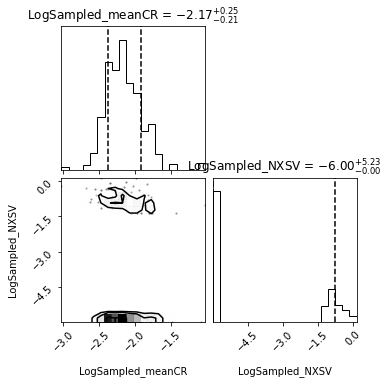
\includegraphics[width=0.47\linewidth]{Figures/Corner_all.png} }}%
    \qquad
    \subfloat{{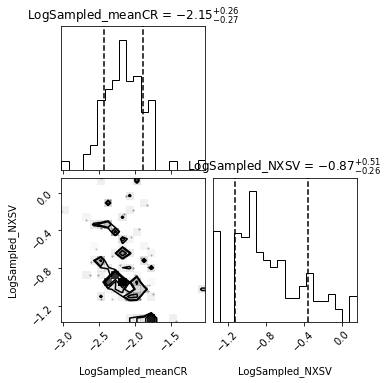
\includegraphics[width=0.47\linewidth]{Figures/Corner_nonzero.png} }}%
     \caption{Αριστερά: Τριγωνικό διάγραμμα \textlatin{(corner plot)} του παραμετρικού χώρου του αλγορίθμου μας- απεικονίζονται οι δύο παράμετροι $(CR_{mean}, \sigma_{rms}^2)$ σε λογαριθμική κλίμακα για όλες τις πηγές του πληθυσμού. Δεξιά: Τριγωνικό διάγραμμα \textlatin{(corner plot)} του παραμετρικού χώρου αποκλείοντας τις πηγές για τις οποίες ο αλγόριθμος απέδωσε την χαμηλότερη τιμη πλάτους μεταβλητότητας $\sigma_{rms, Bayes}^2 =10^{-6}$. Οι διακεκομμένες κατακόρυφες γραμμές ορίζουν το διάστημα γύρω από την μέση τιμή στο οποίο περικλείεται το $68\%$ (περίπου $1\sigma$) της κατανομής κάθε παραμέτρου.}  \label{fig:Corner}
\end{figure*}
  
%-------------------------------------------%
%-------------------------------------------%
%-------------------------------------------%

\section{Αποτελέσματα και σύγκριση με την βάση δεδομένων}

Αποτέλεσμα του αλγόριθμου αυτού με το πακέτο \textlatin{UltraNest} είναι για κάθε μία από τις 210 πηγές μας να έχουμε μία αλυσίδα \textlatin{Markov} me 3000 εως 5000 περίπου δείγματα τιμών $CR_{mean}$ και άλλη μία αλυσίδα \textlatin{Markov} me 3000 εως 5000 περίπου δείγματα τιμών $\sigma_{rms}^2$.

Ως τιμές δειγματοληψίας του αλγορίθμου για τις πηγές μας χρησιμοποιούμε τον αριθμητικό μέσο των τιμών της αλυσίδας $CR_{mean}$ με σφάλμα μέσης τιμής ως αβεβαιότητα και την επικρατούσα τιμή (\textlatin{mode}) των τιμών της αλυσίδας $\sigma_{rms}^2$ με το ελάχιστο διάστημα εμπιστοσύνης $68\%$ ($1\sigma$) του μαζικότερου όγκου της αλυσίδας. Την επικρατούσα τιμή και το διάστημα εμπιστοσύνης τα υπολογίζουμε αφού κάνουμε ένα ιστόγραμμα των καταμετρήσεων των τιμών τις αλυσίδας της διακύμανσης κατανεμημένο σε λογαριθμικό χώρο σε 500 ομάδες \textlatin{(bin)} ίσου λαγαριθμικού πλάτους. Ο μέσος της υψηλότερης \textlatin{bin} του ιστογράμματος θεωρείται η επικρατούσα τιμή \textlatin{(mode)}. Κανονικοποιούμε το ύψος των \textlatin{bin} ώστε να εκφρ'αζεται ώς ποσοστό της μοναδιαίας επιφάνειας του ιστογράμματος κι έπειτα ξεκινώντας από την υψηλότερη \textlatin{bin} συγκρίνουμε τις δύο εγγύτερες της (την εγγύτερη χαμηλότερων τιμών και την εγγύτερη υψηλότερων τιμών) και αθροίζουμε στο ύψος της το ύψος της επικρατέστερης των δύο, επαναλαμβάνουμε μέχρι το άθροισμα αυτό κανονικοποιημένων τιμών να φτάσει το $0.68$ (ελάχιστο διάστημα εμπιστοσύνης). Ως κάτω όριο του διαστήματος εμπιστοσύνης ορίζουμε το μέσο της κάτω χαμηλότερης \textlatin{bin} ενώ ως άνω όριο το μέσο της άνω χαμηλότερης \textlatin{bin} (με κέντρο την επικρατούσα τιμή). Για τις πηγές στις οποίες βρίσκουμε ότι η υψηλότερη \textlatin{bin} (στην οποία τον μέσο θα είχαμε την επικρατέστερη τιμή) έχει ήδη ύψος ίσο ή μεγαλύτερο του $0.68$ και είναι η \textlatin{bin} με τις χαμηλότερες τιμές $\sigma_{rms}^2$ της αλυσίδας δίνουμε ως επικρατούσα τιμή την ελάχιστη $10^{-6}$ kai ως κάτω όριο του διαστήματος εμπιστοσύνης επ'ισης $10^{-6}$. Στο σχήμα \ref{fig:Corner} βλέπουμε την κατανομή του παραμετρικού χώρου δύο διαστάσεων του αλγορίθμου μας. 

\begin{figure*}  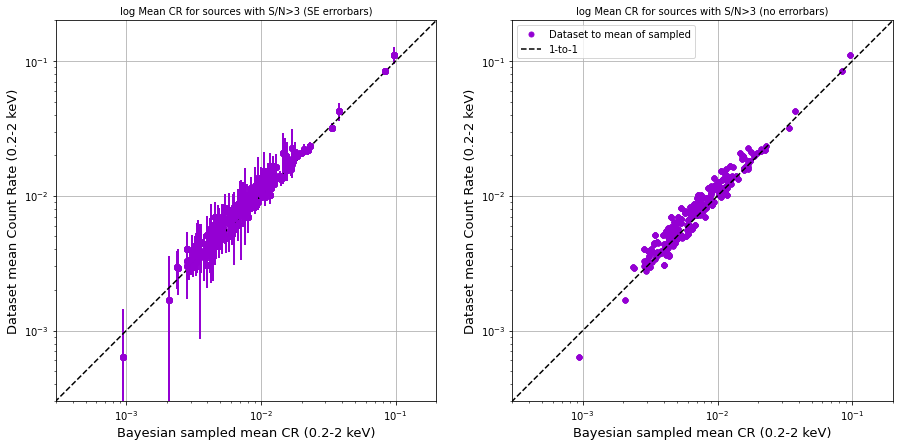
\includegraphics[width=1.12\linewidth]{Figures/Sampled Mean CR.png} \caption{Ο μέσος ρυθμός καταγραφής φωτονίων \textlatin{(mean CR)} όπως υπολογίσαμε από τα δεδομένα αρχείου με τον δειγματοληπτικό \textlatin{(mean CR)} από τον αλγόριθμο. Ως τιμή του δειγματοληπτικού αλγορίθμου έχουμε τον αριθμητικό μέσο της αλυσίδας \textlatin{Markov} κάθε πηγής με το σφάλμα μέσης τιμής ως αβεβαιότητα. Αριστερά έχουμε όλες τις πηγές μαζί με γραμμές σφαλμάτων, ενώ δεξιά έχουμε το ίδιο γράφημα χωρίς τις γραμμές σφαλμάτων.} \label{fig:SampledMeanCR}\end{figure*}

Κάνουμε το γράφημα μέσου ρυθμού καταγραφής φωτονίων της βάσης δεδομένων με τον μέσο ρυθμό καταγραφής φωτονίων που παρήξαμε από τον δειγματοληπτικό αλγόριθμο για να συγκρίνουμε αν τα αποτελέσματα είναι σε συμφωνία (Σχήμα \ref{fig:SampledMeanCR}). Ομοίως και για την παράμετρο $\sigma_{rms}^2$ (Σχήμα \ref{fig:SampledNXSV}).\\
Η τιμή ρυθμού καταγραφής φωτονίων υπολογισμένη από την βάση δεδομένων προκύπτει από την εξίσωση \ref{eq:CR} gia κάθε σημείο καμπύλης φωτός μίας πηγής. Η τιμή του μέσου ρυθμού καταγραφής φωτονίων της βάσης δεδομένων είναι ο αριθμητικός μέσος της ποσότητας \textlatin{CR} για όλα τα σημεία της καμπύλης φωτός μιας πηγής και το αντίστοιχο σφάλμα μέσης τιμής η απεικονιζόμενη αβεβαιότητα.\\
Η τιμή της εγγενούς διακύμανσης $\sigma_{rms}^2$ υπολογισμένη από την βάση δεδομένων (από τις καμπύλες φωτός) προκύπτει από την εξίσωση \ref{eq:NXSV} ενώ η αβεβαιότητα (γραμμές σφάλματος) σε αυτήν προκύπτει από την εξίσωση \ref{eq:NXSVerr} για κάθε πηγή και είναι η \textlatin{NXSV} όπως συζητήθηκε στην παράγραφο 5.2.4. Οι γραμμές σφάλματος για την \textlatin{NXSV} από τον δειγματοληπτικό αλγόριθμο σηματοδοτούν το ελάχιστο διάστημα εμπιστοσύνης ($68\% \; (1 \sigma)$ του μαζικότερου όγκου της αλυσίδας δειγματοληψίας για την \textlatin{NXSV}. Στο σχήμα \ref{fig:SampledNXSV} τα γραφήματα στο πάνω δεξιά \textlatin{panel} και κάτω δεξιά \textlatin{panel} περιέχουν όλες τις πηγές (πάνω με γραμμές σφαλμάτων και κάτω χωρίς γραμμές σφαλμάτων) όμως οι πηγές που έχουν \textlatin{NXSV} (κλασσικά υπολογισμένη ή από αλγόριθμο) με τιμή μικρότερη του $0.005$ εμφανίζονται στα επίπεδα $x=0.0001$ και $y=0.005$, για λόγους εξοικονόμισης χώρου.

\begin{figure*}  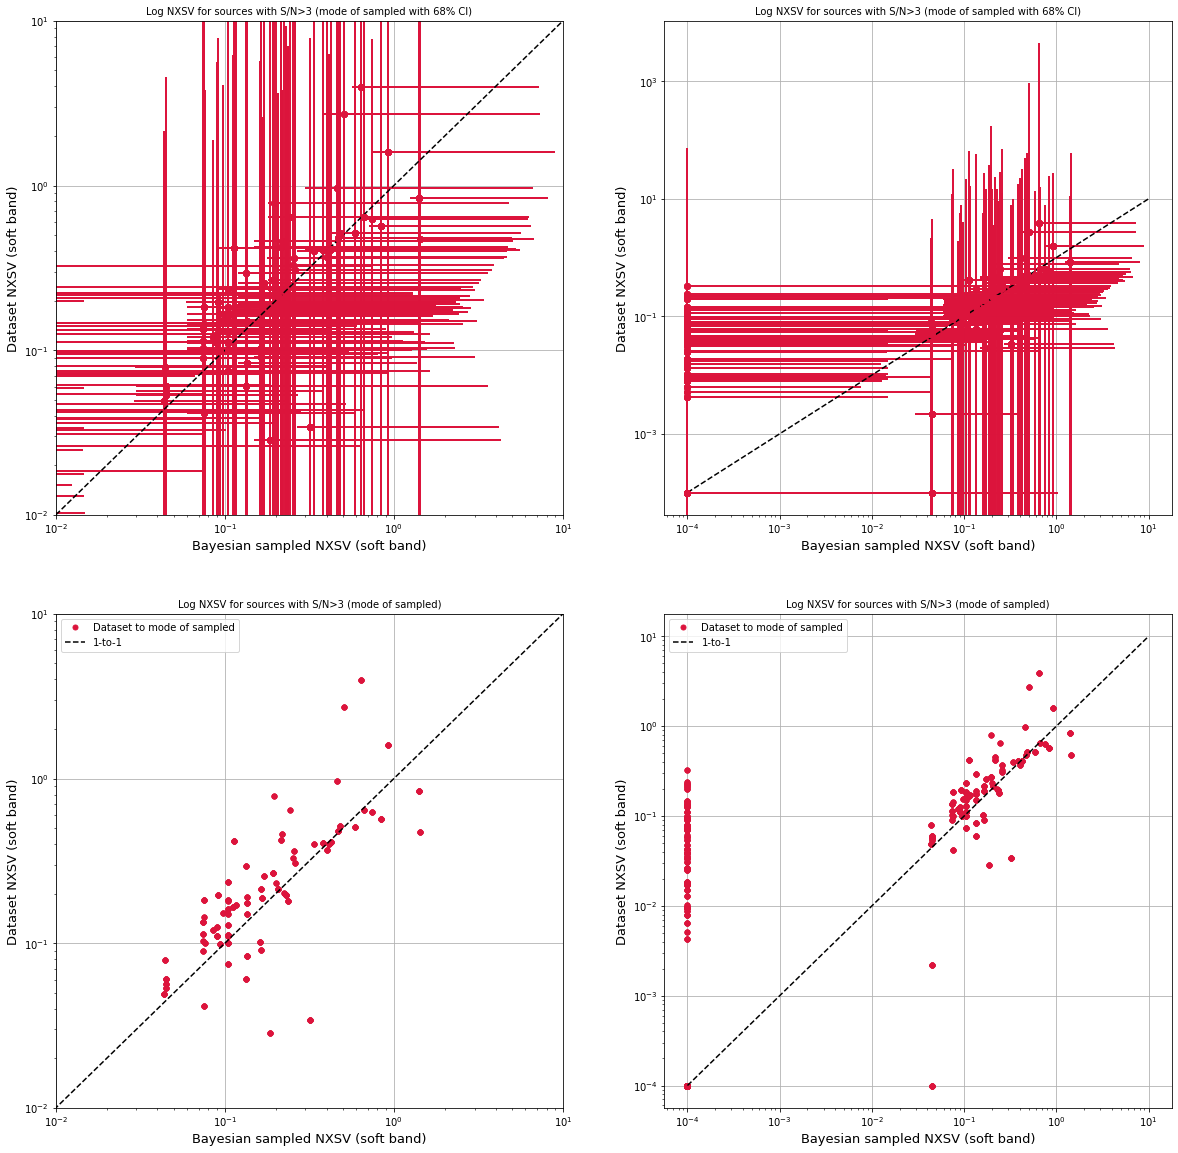
\includegraphics[width=1.12\linewidth]{Figures/Sampled NXSV trunc.png} \caption{H αναλυτική \textlatin{NXSV} όπως υπολογίσαμε από τα δεδομένα αρχείου (σε κάθε κατακόρυφο άξονα) με την \textlatin{NXSV} του δειγματοληπτικού αλγορίθμου συμπερασματολογίας \textlatin{Bayes} (σε κάθε οριζόντιο άξονα). Με διακεκομμένες γραμμές είναι η ένα προς ένα σχέση $y=x$. Ta κάτω πάνελ έχουν ακριβώς τις ίδιες πηγές και εύρος αξόνων με τα ακριβώς από πάνω, δεν έχουν όμως γραμμές σφαλμάτων. Στα πάνω πάνελ, αριστερά έχουμε τον κύριο όγκο των πηγών σε λογαριθμική κλίμακα με εύρος από $10^{-2}$ έως $10$, ενώ δεξιά έχουμε όλες τις πηγές απεικονίζοντας την \textlatin{NXSV} όπου αυτή είναι μικρότερη του $0.005$ στα επίπεδα $y=0.005$ (για την κλασσικά υπολογισμένη) kai $x=0.005$ (για την δειγματοληπτική του αλγορίθμου).} \label{fig:SampledNXSV} \end{figure*}

Παρατηρούμε ότι οι δειγματοληπτικές τιμές με τις κλασσικά υπολογισμένες τιμές συμφωνούν μέσα στα πλαίσια των γραμμών σφαλμάτων. Υπάρχουν πηγές για τις οποίες η δειγματοληπτική μέθοδος προβλέπει μικρότερο πλάτος \textlatin{NXSV} (σημεία στο γράφημα \ref{fig:SampledNXSV} που βρίσκονται πάνω από την γραμή σχέσης 1-1), όμως οι γραμμές σφάλματος περικλείουν την σχέση ταύτησης ένα-προς-ένα.
%({\color{red} νομιζω οτι πρεπει να πεις οτι υπαρχει συμφωνια μεσα στα σφαλματα. Υπαρχουν τιμες που βρισκονται πανω στιν 1-1 σχεση, αλλα και τιμες για τις οποιες η Μπαυζιανη μεθοδος βρισκει πολυ μικροτερο NXSV. Παρόλα'υτα για αυτες τις πηγες το σφαλμα ειναι συμφωνω με την 1-1 σχεση. Ισως αξιζει να βαλεισ τα αρνητικα NXSV στο 1ε-6 και να διξεις οτι υπαρχουν πηγες για τις οποιες η Μπευζιανη προβλεπη μεγαλα NXSV αλλα η κλασσικη μεθοδος οχι}). 

Προχωρούμε στο γράφημα εγγενούς διακύμανσης \textlatin{NXSV} με την λαμπρότητα των πηγών, συγκρίνουμε το γράφημα κλασσικά υπολογισμένης \textlatin{NXSV} με την λαμπρότητα (Σχήμα \ref{fig:ClassicResult}) με το γράφημα της δειγματοληπτικής \textlatin{NXSV} με την λαμπρότητα (Σχήμα \ref{fig:SampledResultB}). Από τις 210 πηγές με παρατηρήσεις απότον ανιχνευτή ΡΝ σε τρείς εποχές και με λόγο σήματος προς θόρυβο $>3$ οι 175 έχουν πληροφορία για ερυθρομετατόπιση (οπότε μόνο για αυτές έχουμε λαμπρότητα).\\ 
Στα γραφήματα αυτά ομαδοποιούμε τις πηγές σε ομάδες των 20 ξεκινώντας από τις χαμηλότερες λαμπρότητες (η τελευταία ομάδα- που αντιστοιχεί σε υψηλότερες λαμπρότητες έχει πάνω από 20 πηγές) και παίρνουμε τον αριθμητικό μέσο της \textlatin{NXSV} για τις συλλογές αυτές των πηγών. Οι γραμμές σφάλματος των σημείων \textlatin{ensemble NXSV} (από συλλογές 20 τουλάχιστον πηγών) προκύπτουν από σφάλμα μέσης τιμής. Αντίστοιχα για κάθε συλλογή υπολογίζεται ο αριθμητικός μέσος της λαμπρότητας. Οι γραμμες σφάλματος για την φωτεινότητα οριοθετούν το εύρος μέγιστης και ελάχιστης λαμπρότητας της συλλογής των πηγών.\\
Και στα δύο γραφήματα φαίνεται η αντισυσχέτιση της \textlatin{NXSV} με την λαμπρότητα, στο σχήμα \ref{fig:SampledResultB} φαίνεται πως για το αποτέλεσμα του αλγορίθμου έχουμε μια αμυδρή κλίση, ενώ στο σχήμα \ref{fig:ClassicResult} (το κλασσικό αποτέλεσμα) η αντισυσχέτιση είναι πιο έκδηλη.
%({\color{red} εξηγησε μεσες τιμες κλπ στα σχηματα}).

\begin{figure*} 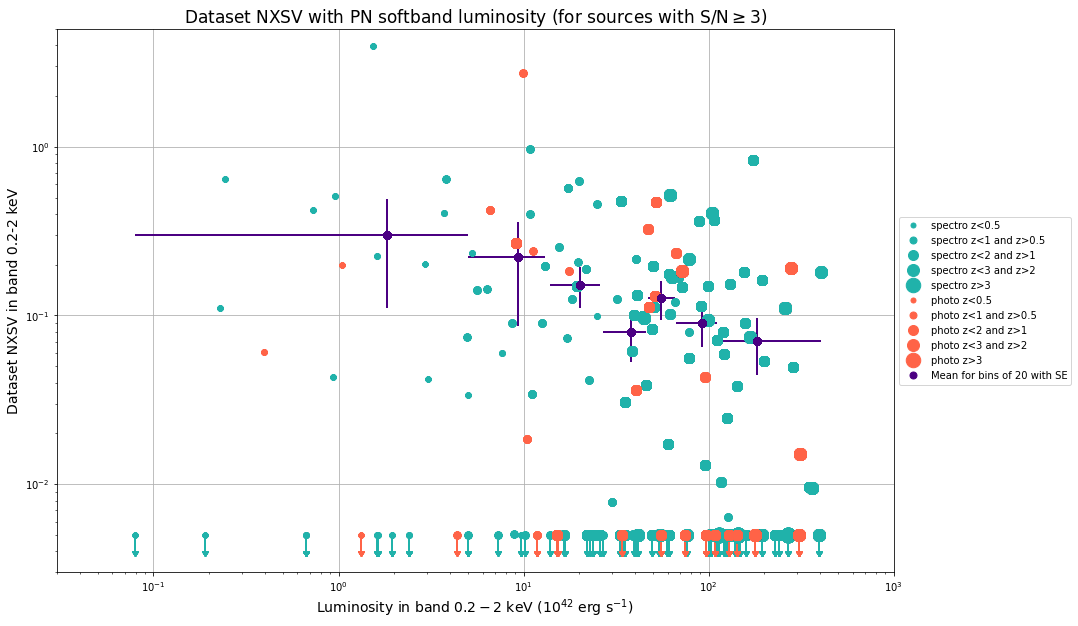
\includegraphics[width=1.12\linewidth]{Figures/Classic NXSV vs Lumi w BINS.png}\caption{H αναλυτική \textlatin{NXSV} όπως υπολογίσαμε από τα δεδομένα αρχείου με λαμπρότητα και \textlatin{binning} κατά λαμπρότητα σε \textlatin{bin} των 20 πηγών με διαφοροποίηση για \textlatin{redshift.}} \label{fig:ClassicResult}  \end{figure*}
 
\begin{figure*} 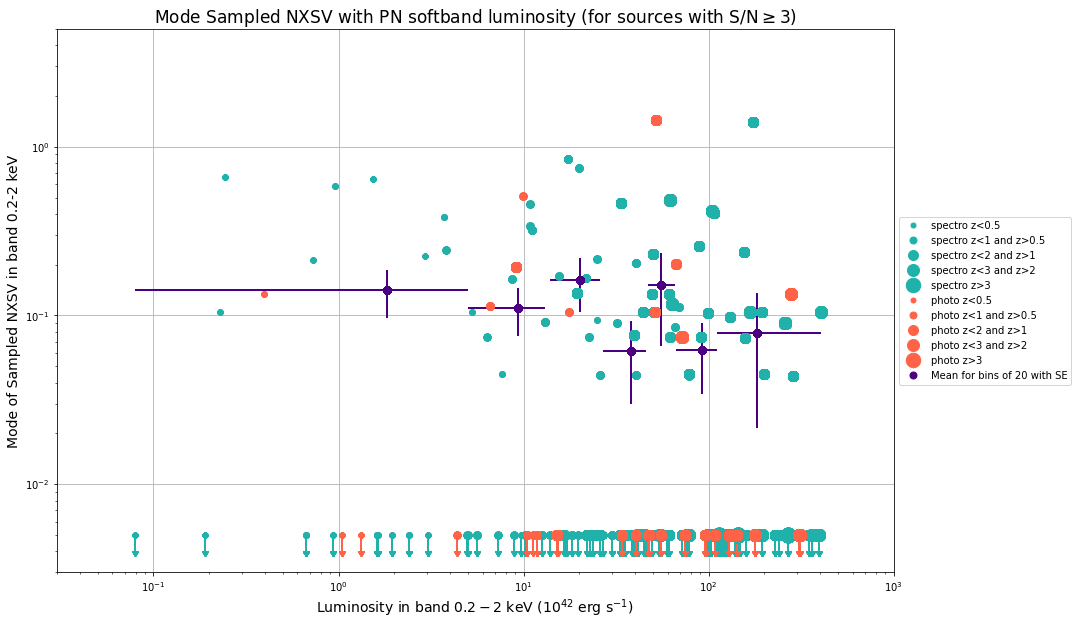
\includegraphics[width=1.12\linewidth]{Figures/Mode Sampled NXSV vs Lumi w BINS B.png} \caption{ Η \textlatin{NXSV} από τον αλγόριθμο \textlatin{Bayes} με λαμπρότητα και \textlatin{binning} κατά λαμπρότητα σε \textlatin{bin} των 20 πηγών με διαφοροποίηση για \textlatin{redshift.}} \label{fig:SampledResultB}  \end{figure*}
 
 
Προβαίνουμε σε στατιστικούς ελέγχους και απλή γραμμική προσαρμογή για να εξετάσουμε την σχέση δειγματοληπτικής \textlatin{NXSV} $\sigma_{rms, Bayes}^2$ με τον λογάριθμο της λαμπρότητας σε μαλακές ακτίνες Χ $\log L_X$. Ως αρχική υπόθεση ($P_{null}$) θεωρούμε ότι δεν υπάρχει συσχέτιση μεταξύ της \textlatin{NXSV} $\sigma_{rms, Bayes}^2$ και του $\log L_X$. Για το στατιστικό τεστ \textlatin{Kendall's} $\tau$ ο συντελεστής συσχέτισης $\sigma_{rms, Bayes}^2$ και $\log L_X$ για τις πηγές με φασματοσκοπικό $z$ είναι $\tau_{spectro} = -0.036$ ενώ για τις πηγές με φωτομετρικό $z$ είναι $\tau_{photo} = -0.053$ τα οποία αντιστοιχούν σε $P_{null, spectro} = 0.539$ kai $P_{null, photo} = 0.682$. Τα αρνητικά πρόσημα στους συντελεστές υποδηλώνουν φθίνουσα μονότονη σχέση, ενώ θεωρούμε ότι υπάρχει (αντι)συσχέτιση αν έχουμε τιμή σημαντικότητας $P_{null}<5\%$, το οποίο δεν ισχύει ούτε για τις πηγές με φασματοσκοπικό ούτε για τις πηγές με φωτομετρικό $z$. Το στατιστικό τεστ \textlatin{Spearman's rank} δίνει συντελεστή συσχέτισης $\rho_{spectro} = -0.048$ me $P_{null, spectro} = 0.573> 0.05$ για τις πηγές με φασματοσκοπικό \textlatin{redshift} kai $\rho_{photo} = -0.074$ me $P_{null, photo} = 0.686>0.05$ για τις πηγές με φωτομετρικό \textlatin{redshift}- δηλαδή δεν έχουμε συσχέτιση της $\sigma_{rms, Bayes}^2$ των πηγών με την λογαριθμική λαμπρότητα $\log L_X$. \\
Για το σύνολο των πηγών (ανεξαρτήτως διαχωρισμού \textlatin{redshift}), το τεστ \textlatin{Kendall's} $\tau$ δίνει συντελεστή συσχέτισης $\tau_{tot} = -0.032$ me $P_{null, tot}= 0.537 >0.05$ ενώ το τεστ \textlatin{Spearman's rank} δίνει συντελεστή συσχέτισης $\rho_{tot} =-0.047$ me $P_{null, tot} = 0.541>0.05$, οπότε και στο σύνολο των πηγών επιβεβαιώνεται η μη-συσχέτιση δειγματοληπτικής \textlatin{NXSV} και λογαριθμικής λαμπρότητας.\\
Για την \textlatin{ensemble NXSV} ο έλεγχος \textlatin{Kendall's} $\tau$ δίνει συντελεστή συσχέτισης $\tau = -0.238$ και ο έλεγχος \textlatin{Spearman's rank} δίνει συντελεστή συσχέτισης $\rho= -0.393$ me τιμές σημαντικότητας $P_{null, \tau} =0.562>0.05$ kai $P_{null, \rho} =0.383>0.05$ αντίστοιχα. Έχουμε δηλαδή μη-συσχέτιση της \textlatin{ensemble NXSV} με την λογαριθμική λαμπρότητα σε επίπεδο σημαντικότητας $95\%$. Η \textlatin{ensemble NXSV} μας επιτρέπει να ελαττώσουμε την διασπορά του δείγματος ώστε να φανεί τυχούσα υποβόσκουσα εξάρτηση. \\ 
Προσαρμόζουμε γραμμική σχέση μέσω γραμμικής παλινδρόμησης (\textlatin{linear regression}) sta δεδομένα και βρίσκουμε κλίση $-0.03$ (δηλαδή $\sigma_{rms, ensemble}^2 = \overline{\sigma_{rms}^2} \propto L_X^{-0.03}$) με σφάλμα μέσης τιμής $StErr = 0.02 $ για την \textlatin{ensemble NXSV}, φυσικά, η κλίση $-0.03$ με σφάλμα μέσης τιμής $0.02$ δεν είναι ικανή να υποστηρίξει συσχέτιση. 

Σε αντίθεση με το κλασσικό αποτέλεσμα, στην περίπτωση της δειγματοληπτικής \textlatin{ensemble NXSV} δεν υποστηρίζεται καμία συσχέτιση με την λαμπρότητα, έτσι συμπεραίνουμε ότι για τον αλγόριθμό που προσαρμόσαμε στα δεδομένα του δείγματός μας, οι \textlatin{AGN} διαφορετικής λαμπρότητας είναι εξίσου μεταβλητοί.\\
Ακόμα κι εδώ, όμως, η αβεβαιότητα των υπολογισμών- τόσο για την εκτίμηση της εγγενούς διακύμανσης κάθε μίας πηγής του δείγματός μας, όσο και τα σφάλαματα μέσης τιμής που αντιστοιχούν στην \textlatin{ensemble NXSV}- είναι τόσο μεγάλη που μας εμποδίζει να έχουμε ένα καταληκτικό συμπέρασμα.  % Experiment 2
	
	\chapter{Μοντέλα μεταβλητότητας}

Προκειμένου να βγάλουμε συμπεράσματα για την σχέση της μεταβλητότητας συλλογών τουλάχιστον 20 πηγών (\textlatin{ensemble NXSV}) με θεμελιώδεις φυσικές παραμέτρους, όπως η μάζα κεντρικής μελανής οπής και ο ρυθμός προσάυξησης, θα συγκρίνουμε με μοντέλα μεταβλητότητας συλλογής \textlatin{AGN} που παρουσιάζονται στην εργασία <<\textlatin{Exploring black-hole scaling relations via the ensemble variability of Active Galactic Nuclei}>> (\textlatin{Georgakakis et al. 2021})\cite{VAR}. Τα μοντέλα αυτά κατασκευάστηκαν με βάση παρατηρησιακές σχέσεις.

%%------------------------%%
%%------------------------%%
%%------------------------%%
\section{Δόμηση μοντέλων μεταβλητότητας}

\begin{figure*}
 \begin{center}
 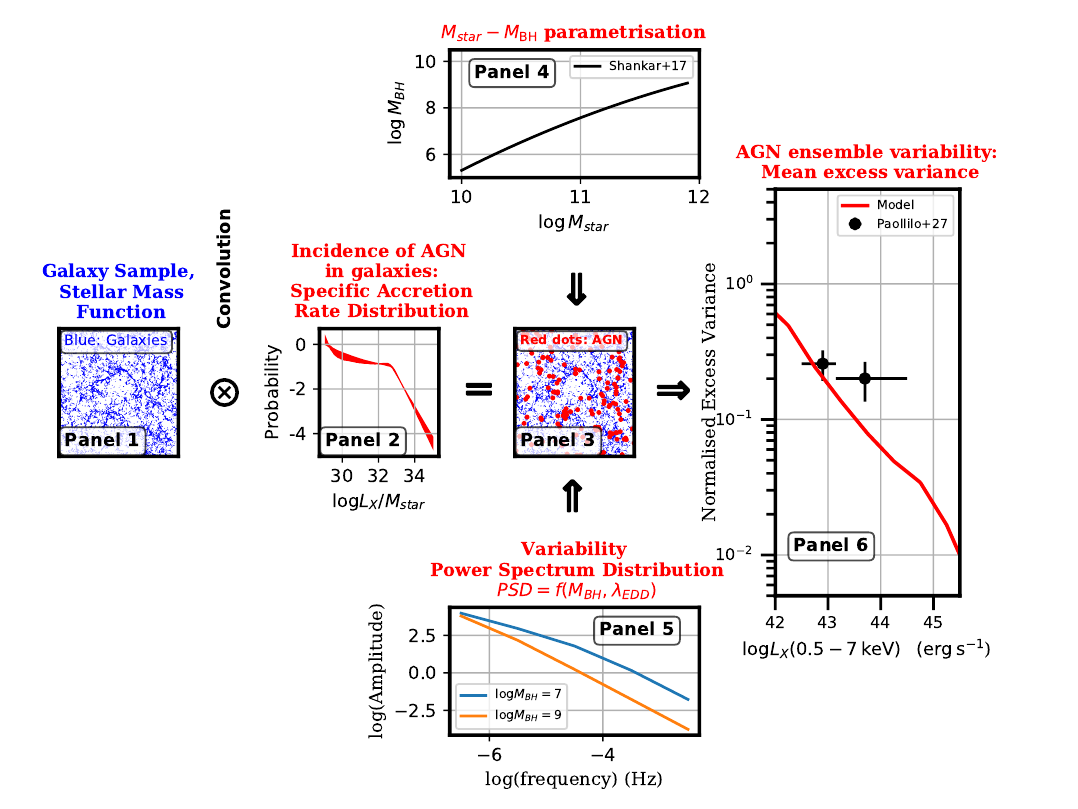
\includegraphics[width=1.1\linewidth]{Figures/ModelConstruction.png}
 \caption{\textlatin{Panel 1}: ογκική πυκνότητα γαλαξιών σε τμήμα κοσμικού ιστού. \textlatin{Panel 2}: πιθανότητα ένας γαλαξίας να έχει συγκεκριμένο ρυθμό προσύξησης. \textlatin{Panel 3}: κατανομή \textlatin{AGN} στην ογκική πυκνότητα γαλαξιών με αντίστοιχες τιμές παραμέτρων ($L_X$, $M_{\star}$, $z$).
 \textlatin{Panel 4}: προσθήκη πληροφορίας $M_{BH}$ και  $\lambda_{Edd}$ για το δείγμα, από την παραμετροποίηση μάζας κεντρικής μελανής οπής με αστρική μάζα γαλαξία και από την σχέση $\lambda_{Edd} \propto L_X/M_{BH}$. 
 \textlatin{Panel 5}: Μορφή συνάρτησης \textlatin{PSD} $\mathcal{P}(f)$ με εξάρτηση από τις φυσικές παραμέτρους του δείγματος (μάζας κεντρικής μελανής οπής $M_{BH}$ και ρυθμό προσύξησης $\lambda_{Edd}$).  
 \textlatin{Panel 6}: Ολοκλήρωση της \textlatin{PSD} στις χρονικές κλίμακες που μελετάμε για ευθύ υπολογισμό πλάτους μεταβλητότητας και σύγκριση με δεδομένα. (Εικόνα από \cite{VAR})}
 \label{fig:ModelConstruction}
 \end{center}
 \end{figure*}

%%------------------------%%

\subsection{Τεχνητός πληθυσμός \textlatin{AGN}}
Η κατασκευή τεχνητού πληθυσμού \textlatin{AGN} ξεκινά από ένα δείγμα γαλαξιών που ακολουθούν συγκεκριμένη συνάρτηση μάζας (όπως αυτό φαίνεται στο \textlatin{Panel 1} του σχήματος \ref{fig:ModelConstruction}) στους οποίους εφαρμόζεται η παρατηρησιακά καθοριζόμενη κατανομή ρυθμών προσαύξησης $\mathbf{p}(\lambda)$ για συγκεκριμένο ρυθμό προσαύξησης $\lambda \propto L_X/ M_{\star}$\cite{VAR}.
Όπου $\lambda$ ο ρυθμός προσαύξησης, $L_X$ η λαμπρότητα στις ακτίνες Χ σε δεδομένο φασματικό παράθυρο και $ M_{\star}$ η αστρική μάζα ενος γαλαξία. Η κατανομή $\mathbf{p}(\lambda)$ μετρά την πιθανότητα ένας γαλαξίας να φιλοξενεί έναν \textlatin{AGN} με ρυθμό προσαύξησης $\lambda \propto L_X/ M_{\star}$ (όπως αυτό φαίνεται στο \textlatin{Panel 2} του σχήματος \ref{fig:ModelConstruction})\cite{VAR}. Ο συγκεκριμένος ρυθμός προσαύξησης αυτός ($\lambda \propto L_X/ M_{\star}$) είναι μια παράμετρος που προκύπτει από παρατηρησιακά δεδομένα και είναι ένα μέτρο του πόση λαμπρότητα στις ακτίνες Χ παράγει ένας \textlatin{AGN} σε σχέση με την αστρική μάζα του γαλαξία που τον <<φιλοξενεί>>. Χρησιμοποιώντας αυτόν τον ρυθμό προσαύξησης στην $\mathbf{p}(\lambda)$, η κατανομή αυτή μας δίνει ένα μέτρο πιθανότητας να υπάρχει ενεργός γαλαξίας ανάμεσα σε πολλούς γαλαξίες. 
%({\color{red} με τη συναρτηση μαζας των γαλαξιων οχι την πυκνοτητα κοσμικου ιστου})
Έτσι η συνέλιξη της κατανομής πιθανότητας να υπάρχει \textlatin{AGN} με την γαλαξιακή πυκνότητα συγκεκριμένης συνάρτησης μάζας, μας δίνει μια χωρική κατανομή \textlatin{AGN} (όπως αυτή φαίνεται στο \textlatin{Panel 3} του σχήματος \ref{fig:ModelConstruction} με υπόβαθρο την γαλαξιακή πυκνότητα)\cite{VAR}. Το αποτέλεσμα είναι να έχουμε παράξει ένα τεχνητό δείγμα \textlatin{AGN} το οποίο είναι συνεπές με την εξελισσόμενη συνάρτηση λαμπρότητας ακτίνων Χ των \textlatin{AGN}, αναπαράγει την παρατηρούμενη συνάρτηση αστρικής μάζας των γαλαξιών με ενεργό γαλαξιακό πυρήνα, την χωρική κατανομή \textlatin{AGN} στον κοσμικό ιστό και τις ιδιότητες των \textlatin{AGN} σε όλα τα μήκη κύματος\cite{VAR}.
Κάθε σημείο στο τεχνητό αυτό δείγμα \textlatin{AGN} έχει αντίστοιχες τιμές λαμπρότητας $L_X$ (για την ενεργειακή μπάντα $2-10$ \textlatin{keV}), αστρικής μάζας γαλαξία $M_{\star}$ και \textlatin{redshift} $z$.

Ακολουθώντας την παραμετροποίηση μάζας κεντρικής μελανής οπής με αστρική μάζα γαλαξία, όπως αυτή φαίνεται στο \textlatin{Panel 4} του σχήματος \ref{fig:ModelConstruction}, αντιστοιχίζουμε σε κάθε \textlatin{AGN} με αστρική μάζα $M_{\star}$ μια τιμή μάζας κεντρικής υπερμεγέθους μελανής οπής $M_{BH}$. Στο τοπικό σύμπαν η αστρική μάζα του κεντρικού σφαιροειδούς των γαλαξιών συσχετίζεται στενά με την μάζα της κεντρικής μελανής οπής \cite{shankar}\cite{savorgnan}, στον αλγόριθμο παραγωγής τεχνητού πληθυσμού και μοντέλων για την \textlatin{ensemble NXSV} χρησιμοποιείται η συσχέτιση\cite{savorgnan}: 
$$\log_{10}\; \frac{M_{BH}}{M_\odot} = 8.35 + 1.31 \cdot \log_{10}\; \big( \frac{M_\star}{M_\odot} -11.0 \big)  $$
για να αντιστοιχίσουμε αστρικές μάζες του κεντρικού σφαιροείδούς με μάζες κεντρικών μελανών οπών. \\
%({\color{red} Αξιζει να πεις οτι στο τοπικο συμπαν η αστρικη μαζα του σφαιροειδους των γαλαξιων συνχετιζετασι στενα με τη μαζα της μαυρηα τρυπας και οτι αυτη τη συσχετηση χρησμοποιεις για να αντιστοιχισεις αστρικες μαζεσ μς μελανς οπες}).
Κατ> επέκταση, για κάθε τιμή φωτεινότητας $L_X$ που διαθέτουμε, αντιστοιχίζουμε μια τιμή πηλίκου \textlatin{Eddington} $\lambda_{Edd}$ σε κάθε ενεργό γαλαξιακό πυρήνα, me $\lambda_{Edd} \propto L_X/L_{Edd} \iff \lambda_{Edd} \propto L_X/M_{BH}$ , όπου $L_{Edd}$ η βολομετρική λαμπρότητα \textlatin{Eddington} (στην έκφραση του πηλίκου έχουμε και παράγοντα βολομετρικής διόρθωσης\cite{duras2020} τον οποίο λαμβάνει υπ> όψιν ο αλγόριθμος).  
%()({\color{red} Λειπει το bolometric correction, δηλαδη η συνολικη λαμπροτητα που εκπεμπει η ενεργη μελανη οπη η οποια σχετιζεται προφανως με ην λαμπροτητα-Χ αλλα. Οποτε στην απλη περιπτωση που ν λαμπροτητα-Χ ειναι αναλαογη της βολομετρικης τοτε σου λειπει ενας παραγοντας για να γινει η πιο πανω αναλογια ισοτητα})..
Οι στοχαστικές μεταβολές στην λαμπρότητα των \textlatin{AGN} που θέλουμε να μελετήσουμε σε διάφορες χρονικές κλίμακες περιγράφονται ποσοτικά από την \textlatin{PSD} $\mathcal{P}(f)$, δηλαδή την κατανομή της διακύμανσης της καμπύλης φωτός σε συχνότητες \textlatin{Fourier} (όπως αυτή φαίνεται στο \textlatin{Panel 5} του σχήματος \ref{fig:ModelConstruction}).
Η ολοκλήρωση της \textlatin{PSD} στις χρονικές κλίμακες που θέλουμε να μελετήσουμε καθορίζει το πλάτος μεταβλητότητας (\textlatin{NXSV}) των αντίστοιχων \textlatin{AGN} του δείγματος. Το πλάτος μεταβλητότητας κάθε \textlatin{AGN} του τεχνητού δείγματος ομαδοποιείται κατά λαμπρότητα και έτσι προκύπτει η \textlatin{ensemble NXSV} (όπως φαίνεται με συνεχή γραμμή στο \textlatin{Panel 6} του σχήματος \ref{fig:ModelConstruction}) και συγκρίνεται άμεσα με τα παρατηρησιακά αποτελέσματα (κουκίδες στο \textlatin{Panel 6} του σχήματος \ref{fig:ModelConstruction})\cite{VAR}. 

%%------------------------%%

\subsection{Μοντελοποίηση \textlatin{PSD} και πλάτος μεταβλητότητας (\textlatin{NXSV})}

Παρατηρήσεις δείχνουν ότι οι \textlatin{PSD} κοντινών \textlatin{AGN} τύπου \textlatin{Seyfert} (μια από τις μεγαλύτερες κατηγορίες ενεργών γαλαξιακών πυρήνων) μπορούν να προσεγγιστούν πρακτικά με μορφή κυρτωμένου νόμου δύναμης \textlatin{(broken power-law)} του οποίου οι παράμετροι (κλίση, συχνότητα αποκοπής, παράγοντας κανονικοποίησης) εξαρτώνται από φυσικές ιδιότητες του συστήματος (όπως είναι η μάζα κεντρικής υπερμεγέθους μελανής οπής και ρυθμός προσαύξησης)\cite{2012A&A...542A..83P} \cite{VAR}. Θα υιοθετήσουμε την εξής μορφή για την συνάρτηση πυκνότητας φασματικής ενεργειακής ισχύος \textlatin{PSD} των \textlatin{AGN}\cite{2012A&A...544A..80G} \cite{2017MNRAS.471.4398P}, η οποία βασίζεται σε φασματικές μελέτες κοντινών \textlatin{AGN}:
 \begin{equation} \mathcal{P}(f) = A\cdot f^{-1} \big( 1+\dfrac{f}{f_b}   \big)^{-1} \label{eq:PSDform}\end{equation}
Όπου $Α$ ο παράγοντας κανονικοποίησης και $f_b$ η συχνότητα αποκοπής. Εδώ η \textlatin{PSD} έχει λογαριθμική κλίση $-1$ για $f\ll f_b$ kai $-2$ gia $f\gg f_b$.\\
 Θα εξετάσουμε τέσσερεις διαφορετικές εμπειρικές σχέσεις που συσχετίζουν την μορφή της \textlatin{PSD} με την μάζα κεντρικής υπερμεγέθους μελανής οπής $M_{BH}$ και το πηλίκο \textlatin{Eddington} $\lambda_{Edd}$ ενός \textlatin{AGN}, οπότε μοντελοποιούμε την \textlatin{PSD} (σχέση \ref{eq:PSDform}) ως εξής\cite{2017MNRAS.471.4398P}:

\begin{itemize}
    \item \textbf{Μοντέλο 1}: Το πλάτος της \textlatin{PSD} στην συχνότητα αποκοπής $f_b$ είναι σταθερό σύμφωνα με την σχέση $$f_b \times  \mathcal{P}(f) = 0.02$$ για όλους τους  \textlatin{AGN}. Ενώ η συχνότητα αποκοπής εξαρτάται από την μάζα μελανής οπής σύμφωνα με την σχέση $$f_b = 580/(M_{BH} /M_{\odot} ) \; \mbox{\textlatin{s}}^{-1} $$

    \item \textbf{Μοντέλο 2}: Το πλάτος της \textlatin{PSD} στην συχνότητα αποκοπής $f_b$ είναι σταθερό όπως στο Μοντέλο 1, ενώ η συχνότητα αποκοπής εξαρτάται και από την μάζα μελανής οπής και από τον ρυθμό προσαύξησης σύμφωνα με την σχέση $$f_b = (200/86400)(L_{44,bol} )(M_{6,BH} )^{−2} \; \mbox{\textlatin{s}}^{-1} $$ όπου η $L_{44,bol}$ είναι η βολομετρική φωτεινότητα σε μονάδες $10^{44} \; \mbox{\textlatin{erg}}  \mbox{  \textlatin{s}}^{-1}$ kai $M_{6,BH}$ είναι η μάζα μελανής οπής σε μονάδες $10^{6}\; M_{\odot}$.

    \item \textbf{Μοντέλο 3}: Η συχνότητα αποκοπής εξαρτάται από την μάζα μελανής οπής σύμφωνα με την σχέση $$f_b = 580/(M_{BH} /M_{\odot} )\; \mbox{\textlatin{s}}^{-1} $$ όπως στο Μοντέλο 1. Ομως ο παράγοντας κανονικοποίησης της \textlatin{PSD} εξαρτάται από τον ρυθμό προσαύξησης σύμφωνα με την σχέση $$f_b \times  \mathcal{P}(f) = 3 \cdot 10^{-3} \lambda_{Edd}^{-0.8}$$ 
    
    \item \textbf{Μοντέλο 4}: Όπως και στο Μοντέλο 2, η συχνότητα αποκοπής εξαρτάται από την μάζα μελανής οπής και από τον ρυθμό προσαύξησης σύμφωνα με την σχέση $$f_b = (200/86400)(L_{44,bol} )(M_{6,BH} )^{−2}\; \mbox{\textlatin{s}}^{-1} $$ αλλά ο παράγοντας κανονικοποίησης της \textlatin{PSD} εξαρτάται από τον ρυθμό προσαύξησης σύμφωνα με την σχέση $$f_b \times  \mathcal{P}(f) = 3 \cdot 10^{-3} \lambda_{Edd}^{-0.8}$$ όπως στο Μοντέλο 3.

\end{itemize}

Στα Μοντέλα 1 και 3 η συχνότητα αποκοπής εξαρτάται μόνο από την μάζα κεντρικής μελανής οπής, γι> αυτό και στο σχήμα \ref{fig:BiasModels} βλέπουμε ότι κατανείμεται σταθερά με την λαμπρότητα, ενώ το ίδιο δεν συμβαίνει για τα Μοντέλα 2 και 4 τα οποία εξαρτώνται από την βολομετρική λαμπρότητα $L_{bol}$ (η οποία έχει συνιστώσα $L_X$) ή από το πηλίκο \textlatin{Eddington} $\lambda_{Edd} \propto L_{X}/M_{BH}$, γι> αυτό και στο διάγραμμα του σχήματος \ref{fig:BiasModels} φαίνεται η εξάρτηση της συχνότητας αποκοπής από την λαμπρότητα $L_X$.  
 
Έχοντας τιμές για λαμπρότητα στις ακτίνες Χ, αστρική μάζα γαλαξία, \textlatin{redshift}, μάζα κεντρικής υπερμεγέθους μελανής οπής και πηλίκο \textlatin{Eddington} ($L_X$, $M_{\star}$, $z$, $M_{BH}$, $\lambda_{Edd}$) για κάθε \textlatin{AGN} του τεχνητού δείγματός μας, μοντελοποιούμε το πλάτος μεταβλητότητας $\sigma_{rms}^2$ για κάθε ξεχωριστό \textlatin{AGN} και για συλλογή \textlatin{AGN} (\textlatin{ensemble NSXV}). Για κάθε ξεχωριστό μοντέλο \textlatin{PSD} που χρησιμοποιούμε (από τα Μοντέλα 1,2,3,4), και δεδομένες τις παραμέτρους ($L_X$, $M_{\star}$, $z$, $M_{BH}$, $\lambda_{Edd}$) για κάθε \textlatin{AGN} του τεχνητού δείγματός υπολογίζουμε την ποσότητα\cite{2017MNRAS.471.4398P}:
\begin{equation} \begin{aligned} \sigma_{rms, mod}^2 = {} & \int_{f_{min}}^{f_{max}} \mathcal{P}(f)df \\ & = A \cdot \Big[ ln \Big( \dfrac{f_{max}}{f_{min}} \Big) - ln \Big(   \dfrac{f_b + f_{max}}{f_b + f_{min}}  \Big)   \Big] \label{eq:NXSVmod} \end{aligned}\end{equation}

%%------------------------%%
%%------------------------%%
%%------------------------%%
\section{Προσαρμογή μοντέλων στο δείγμα μας και σύγκριση}

Τα παραπάνω μοντέλα έχουν κάποιες ελεύθερες παραμέτρους (χρονικές κλίμακες ολοκλήρωσης της \textlatin{PSD} για τον υπολογισμό πλάτους μεταβλητότητας $\sigma_{rms, mod}^2$), αλλά και παραμέτρους που μπορούμε να προσαρμόσουμε ώστε να συμπίπτουν με τα χαρακτηριστικά του πληθυσμού \textlatin{AGN} του πεδίου \textlatin{XMM-XXL-North} που μελετάμε (ενεργειακό παράθυρο φλαμπρότητας, εύρος ερυθρομετατοπίσεων).\\ 
Χρησιμοποιούμε το εργαλείο \textlatin{WebPIMMS} για να μετατρέψουμε την λαμπρότητα του τεχνητού δείγματος από $2-10$ \textlatin{keV} σε $0.2-2$ \textlatin{keV} κάνοντας την παραδοχή φασματικού δείκτη $1.9$ σε πρώτη προσέγγιση νόμου δύναμης της \textlatin{PSD} των \textlatin{AGN}\cite{PIMMS}. Επίσης προσαρμόζουμε το δείγμα αυτό σε ερυθρομετατοπίσεις από $z_{min, mod}=0$ έως $z_{max, mod}=4$.\\
Έπειτα, για κάθε μοντέλο \textlatin{PSD} που εφαρμόζουμε, υπολογίζουμε πλάτος μεταβλητότητας $\sigma_{rms, mod}^2$ ολοκληρώνοντας την εκάστοτε συνάρτηση \textlatin{PSD} $\mathcal{P}(f)$ με άκρα ολοκλήρωσης που αντιστοιχούν σε χρονικές κλίμακες $f_{max} =1/Τ_{min, mod}$ και  $f_{min} =1/Τ_{max, mod}$.
\begin{figure*}%
    \centering
    \subfloat{{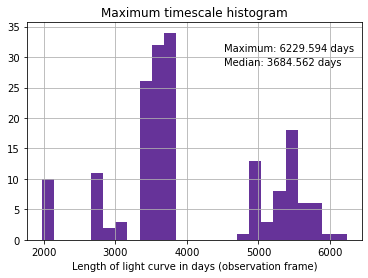
\includegraphics[width=0.46\linewidth]{Figures/MaxTimescale.png} }}%
    \qquad
    \subfloat{{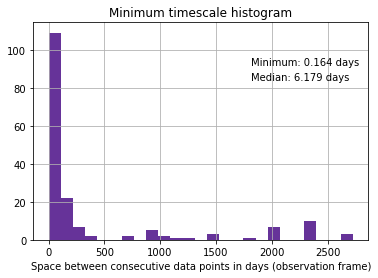
\includegraphics[width=0.46\linewidth]{Figures/MinTimescale.png} }}%
     \caption{Ιστογράμματα των μέγιστων και ελάχιστων χρονικών κλιμάκων. Αριστερά: ιστόγραμμα κατανομής των μηκών καμπύλων φωτός για όλες τις πηγές του πεδίου \textlatin{XMM-XXLL-N} που μελετάμε στο αδρανειακό σύστημα παρατήρησης, με τον διάμεσο αυτών να αποτελεί την μέγιστη χρονική κλίμακά μας. Δεξιά: ιστόγραμμα κατανομής των διαστημάτων μεταξύ διαδοχικών σημείων καμπύλων φωτός για όλες τις πηγές του πεδίου \textlatin{XMM-XXLL-N} που μελετάμε στο αδρανειακό σύστημα παρατήρησης, με τον διάμεσο αυτών να αποτελεί την ελάχιστη χρονική κλίμακά μας.} \label{fig:MaxMInTime}
\end{figure*}
 
Ως μέγιστη κλίμακα χρόνου $Τ_{max, mod}= 1/f_{min}$ για το μοντέλο μας επιλέγουμε το μέγιστο χρονικό διάστημα $\Delta T_{lightcurve}$ που εκτείνεται η καμπύλη φωτός μιας πηγής (απόσταση του πρώτου από το τελευταίο σημείο), όπως το καταγράφουμε στο αδρανειακό σύστημα παρατήρησης. Για τις πηγές του πεδίου που μελετάμε, η μέγιστη αυτή χρονική κλίμακα σε σύστημα ηρεμίας είναι $Τ_{max, mod}= 3684.562 \mbox{\textlatin{ days}}$ (όπως φαίνεται στο σχήμα \ref{fig:MaxMInTime}). Aυτός είναι ο διάμεσος του μήκους των καμπυλών φωτός στο σύστημα παρατήρησης του πληθυσμό που μελετάμε.\\
Ως ελάχιστη κλίμακα χρόνου $Τ_{min, mod}= 1/f_{max}$ για τα μοντέλα μας επιλέγουμε το ελάχιστο χρονικό διάστημα μεταξύ διαδοχικών σημείων μιας καμπύλης φωτός, για τις καμπύλες φωτός των πηγών του δείγματός μας όπως το καταγράφουμε στο αδρανειακό σύστημα παρατήρησης. Βρίσκουμε τον αριθμητικό διάμεσο των διαστημάτων μεταξύ διαδοχικών σημείων καπμύλων φωτός ο οποίος είναι $Τ_{min, mod}=6.179  \mbox{\textlatin{ days}}$ (όπως φαίνεται στο σχήμα \ref{fig:MaxMInTime}). 
Έτσι στην  εφαρμογή των μοντέλων που κάνουμε χρησιμοποιούμε ως μέγιστη χρονική κλίμακα $Τ_{max, mod}= 3684.562 \mbox{\textlatin{ days}}$ και ως ελάχιστη χρονική κλίμακα $Τ_{min, mod}= 6.179  \mbox{\textlatin{ days}}$. \\
Εισάγουμε τους χρόνους στο σύστημα παρατήρησης, αφού ο αλγόριθμος της εργασίας \cite{VAR} αναλαμβάνει διορθώσεις για το αδρανειακό σύστημα ηρεμίας των πηγών.

Όπως έχει επισημανθεί, σύμφωνα με μελέτες\cite{2013ApJ...771....9A}, η μεροληψία (\textlatin{bias}) στην εκτίμηση της \textlatin{ensemble NXSV} είναι σημαντική όταν η ελάχιστη συχνότητα ολοκλήρωσης (που συνδέεται με την μέγιστη χρονική κλίμακα $f_{min} =1/Τ_{max, mod}$) είναι μεγαλύτερη της συχνότητας αποκοπής $f_b$ των \textlatin{PSD} των μοντέλων. 
H ελάχιστη συχνότητα για την μελέτη μας είναι $$f_{min} =\frac{1}{Τ_{max, mod}} = \frac{1}{3684.562 \mbox{\textlatin{ days}} } = 3.1 \times 10^{-9}\; \mbox{\textlatin{s}}^{-1}$$ 
Για κάθε ένα μοντέλο κάνουμε το διάγραμμα πυκνότητας της συχνότητας αποκοπής $f_b$ με την λαμπρότητα $L_X$ στο ενεργειακό παράθυρο $0.2-2$ \textlatin{keV} χαράζοντας και το επίπεδο $f_{min} = 3.1 \times 10^{-9}$ \textlatin{s}$^{-1}$. Εξετάζουμε έτσι αν υπάρχει σημαντική μεροληψία στον υπολογισμό μας.
\begin{figure*}%
    \centering
    \subfloat{{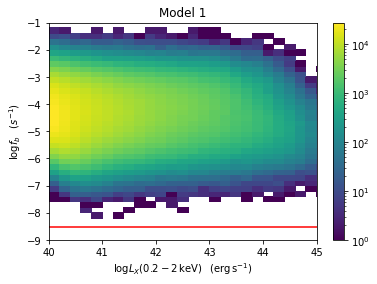
\includegraphics[width=0.46\linewidth]{Figures/Model 1 obs.png} }}%
    \qquad
    \subfloat{{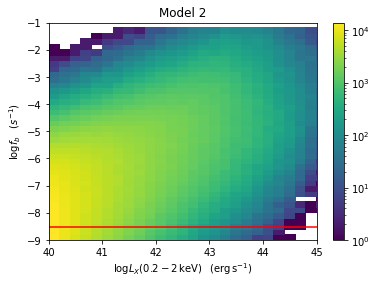
\includegraphics[width=0.46\linewidth]{Figures/Model 2 obs.png} }}%
    \vspace{4ex}
    \subfloat{{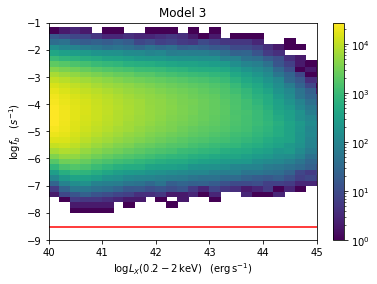
\includegraphics[width=0.46\linewidth]{Figures/Model 3 obs.png} }}
    \qquad
    \subfloat{{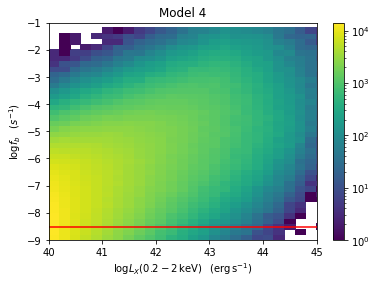
\includegraphics[width=0.46\linewidth]{Figures/Model 4 obs.png} }} \caption{Διαγράμματα πυκνότητας της συχνότητας αποκοπής $f_b$ (κατακόρυφος άξονας) με λαμπρότητα $L_X$ στο ενεργειακό παράθυρο $0.2-2$ \textlatin{keV} για κάθε ένα από τα τέσσερα Μοντέλα (σε κάθε πάνελ), η συχνότητα αποκοπής έχει μετασχηματιστεί για το αδρανειακό σύστημα παρατήρησης. Η κόκκινη γραμμή αντιπροσωπεύει την ελάχιστη συχνότητα ολοκλήρωσης της \textlatin{PSD:} $f_{min} = 3.1 \times 10^{-9}$ \textlatin{s}$^{-1}$ η οποία βασίζεται στην μέση μέγιστη χρονική κλίμακα στο σύστημα παρατήρησης. Οι άξονες του γραφήματος είναι σε λογαριθμική κλίμακα.} \label{fig:BiasModels}
\end{figure*}
 
'Οπως φαίνεται από το σχήμα \ref{fig:BiasModels}, gia τα Μοντέλα 1 και 3 δεν έχουμε σημαντικό \textlatin{bias} στον υπολογισμό της $\sigma_{rms}^2$, όμως για τα Μοντέλα 2 και 3 στις λαμπρότητες $10^{40}-10^{45}$ \textlatin{erg  s}$^{-1}$ βλέπουμε ότι έχουμε συχνότητες αποκοπής μικρότερες της ελάχιστης συχνότητας ολοκλήρωσης, οπότε έχουμε σημαντικό \textlatin{bias} στον υπολογισμό της $\sigma_{rms}^2$ από φαινόμενα \textlatin{aliasing} από χαμηλότερες συχνότητες. Ο αλγόριθμος που υπολογίζει την \textlatin{ensemble NXSV} me ολοκλήρωση των \textlatin{PSD} διορθώνει την $\sigma_{rms}^2$ με πολλαπλασιαστικό παράγοντα $C \cdot 0.48^{\beta-1}$, λαμβάνοντας τιμές $C = 1.3$ kai $\beta = 1.1$. 

Καταλήγουμε στην παραγωγή τεχνητού δείγματος \textlatin{AGN} με \textlatin{redshift} $z \in [0,4]$ kai λαμπρότητα $L_X$ στο ενεργειακό παράθυρο $[0.2 \mbox{\textlatin{keV}}\;, 2 \; \mbox{\textlatin{keV}}]$ για κάθε μοντέλο \textlatin{PSD}, για το οποίο υπολογίζουμε πλάτος μεταβλητότητας $\sigma_{rms, mod}^2$  ολοκληρώνοντας τις \textlatin{PSD} των μοντέλων για παρατηρούμενες χρονικές κλίμακες $Τ_{min, mod}= 6.179 \mbox{\textlatin{ days}}$ kai $Τ_{max, mod} = 3684.562  \mbox{\textlatin{ days}}$. Συνυπολογίζεται διόρθωση \textlatin{bias}. 
 
\begin{figure*}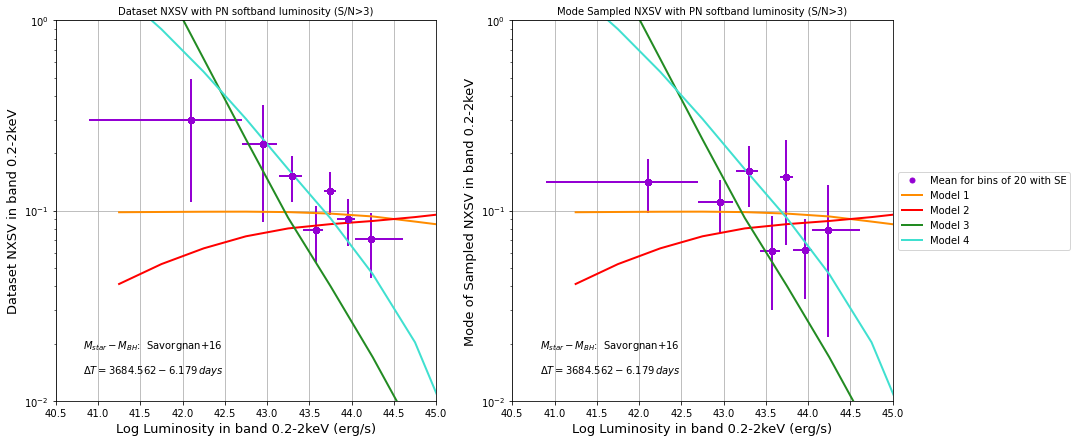
\includegraphics[width=1.1\linewidth]{Figures/ModelsFINAL.png}\caption{Αριστερά: η \textlatin{NXSV} όπως υπολογίσαμε από τα δεδομένα αρχείου με λαμπρότητα και \textlatin{binning} κατά λαμπρότητα σε \textlatin{bin} των 20 πηγών με διαφοροποίηση για \textlatin{redshift} και τα Μοντέλα 1, 2, 3, 4 διαφοροποιούνται στην μορφή της \textlatin{PSD} όπως έχει επισημανθεί, η ελάχιστη χρονική κλίμακα μεταβλητότητας είναι $Τ_{min, mod}=  6.179 \mbox{\textlatin{ days}}$, δηλαδή ο διάμεσος των μικρότερων χρονικών αποστάσεων ηρεμίας διαδοχικών σημείων καμπύλης φωτός μεταξύ των πηγών και η μέγιστη χρονική κλίμακα είναι η μέγιστη όλων των καμπύλων φωτός $Τ_{max, mod}=  3684.562 \mbox{\textlatin{ days}}$. Δεξιά: η \textlatin{NXSV} από τον αλγόριθμο \textlatin{Bayes} όπως έχει περιγραφεί με λαμπρότητα και τα ίδια ακριβώς φασματικά μοντέλα. }  \label{fig:ModelsFinal} \end{figure*}

\begin{figure*}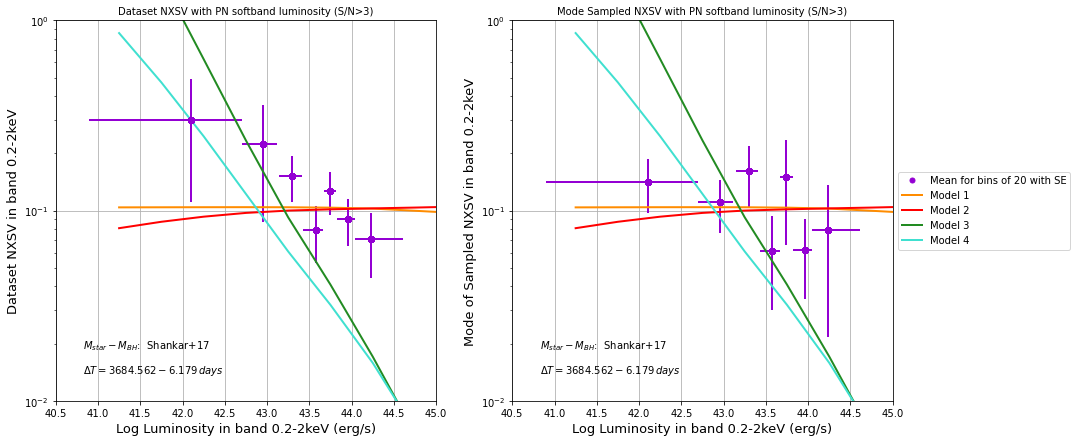
\includegraphics[width=1.1\linewidth]{Figures/ModelsFINALshankar.png}\caption{Αριστερά: η \textlatin{NXSV} όπως υπολογίσαμε από τα δεδομένα αρχείου με λαμπρότητα και \textlatin{binning} κατά λαμπρότητα σε \textlatin{bin} των 20 πηγών με διαφοροποίηση για \textlatin{redshift} και τα Μοντέλα 1, 2, 3, 4 διαφοροποιούνται στην μορφή της \textlatin{PSD} όπως έχει επισημανθεί, εδώ αυτή τη φορά αντί να χρησιμοποιήσουμε την σχέση αστρικής μάζας με μάζα μελανής οπής όπως προτείνεται από την εργασία \cite{savorgnan}, χρησιμοποιούμε την συσχέτιση μαζών σύμφωνα με την εργασία \cite{shankar}. Δεξιά: η \textlatin{NXSV} από τον αλγόριθμο \textlatin{Bayes} όπως έχει περιγραφεί με φωτεινότητα και τα ίδια ακριβώς φασματικά μοντέλα. }  \label{fig:ModelsFinalshankar} \end{figure*}

Στο σχήμα \ref{fig:ModelsFinal} χαράσουμε την σχέση πλάτους μεταβλητότητας με λαμπρότητα στις μαλακές ακτίνες Χ για κάθε μοντέλο (συνεχής γραμμή με χρωματικό κώδικα για Μοντέλο 1, Μοντέλο 2, Μοντέλο 3, Μοντέλο 4) για το τεχνητό δείγμα \textlatin{AGN} με τα χαρακτηριστικά που συζητήσαμε, και τοποθετούμε την \textlatin{ensemble NXSV} για ομάδες 20 τουλάχιστον πηγών του πληθυσμό \textlatin{AGN} του πεδίου \textlatin{XMM-XXL-North} όπως την υπολογίσαμε από δεδομένα αρχείου (επιλέγοντας πηγές με λόγο \textlatin{S/N}$>3$ και με διαθέσιμη τιμή \textlatin{redshift}) kai την \textlatin{ensemble NXSV} για ομάδες 20 τουλάχιστον \textlatin{AGN} από τον δειγματολογικό αλγόριθμο \textlatin{Bayes} που βασίσαμε στις πηγές του πληθυσμού \textlatin{AGN} του πεδίου \textlatin{XMM-XXL-North}. Στο σχήμα \ref{fig:ModelsFinal} η συνάρτηση αστρικής μάζας κεντρικού σφαιροειδούς με την μάζα υπερμεγέθους μελανής οπής που χρησιμοποιήθηκε στον τεχνητό πληθυσμό μας είναι η (\textlatin{Savorgnan})\cite{savorgnan} 
$$ \log_{10} \frac{M_{BH}}{M_\odot} = 8.35 +1.31 (\log_{10} \frac{M_\star}{M_\odot} +11.0) $$
ενώ, για σύγκριση, χαράσουμε το ίδιο διάγραμμα στο σχήμα \ref{fig:ModelsFinalshankar} ακολουθώντας για τον πληθυσμό μας την εναλλακτική σχέση (\textlatin{Shankar})\cite{shankar} 
$$ \log \frac{M_{BH}}{M_\odot} = 7.574 +  1.946(\log \frac{M_\star}{M_\odot} +11.0)  -0.306(\log \frac{M_\star}{M_\odot} +11.0)^2 -0.011(\log \frac{M_\star}{M_\odot} +11.0) ^3 $$

%(Στην εργασία αυτή, όταν χρησιμοποιούμε το σύμβολο του λογαρίθμου εννοούμε δεκαδικό λογάριθμο- εκτός αν τονίζεται διαφορετικά.)\\
Παρατηρούμε ότι στην περίπτωση του κλασσικού υπολογισμού της \textlatin{ensemble NXSV} από την βάση δεδομένων το Μοντέλο 1 περνά από τις γραμμές σφαλμάτων 5 σημείων απο τα 7, ενώ το Μοντέλο 4 περνά από τις γραμμές σφάλματος 4 σημείων από τα 7. Στον υπολογισμό της \textlatin{ensemble NXSV} από τον δειγματοληπτικό αλγόριθμο συμπερασματολογίας \textlatin{Bayes} τόσο το Μοντέλο 1 όσο και και το Μοντέλο 4 περνούν από τις γραμμές σφάλματος 4 σημείων από τα 7 (αναφερόμαστε πρωτίστως στα μοντέλα με χρήση της σχέσης μάζας \textlatin{Savorgnan} που θεωρείται πιο έγκυρη- χρησημοποιούμε την σχέση μάζας \textlatin{Shankar} αμιγώς για σύγκριση).

Λόγω των μεγάλων σφαλμάτων των μετρήσεων είναι δύσκολο να βγάλουμε συμπεράσματα για το ποιό μοντέλο περιγράφει καλύτερα τα δεδομένα μας.\\
Εφαρμόζουμε το στατιστικό τεστ $\chi^2$ καλύτερης προσαρμογής, το οποίο λαμβάνει υπ> όψιν την αβεβαιότητα στις μετρήσεις ως εξής
$$ \chi^2 = \sum_{i=1}^N \Big( \dfrac{x_{obs} - x_{model}}{\sigma_i} \Big)^2$$
με $x_{obs}$ τις μετρήσεις της \textlatin{ensemble NXSV}, $x_{model}$ την τιμή της \textlatin{NXSV} που προτείνει το εκάστοτε μοντέλο για την ίδια λαμπρότητα και $\sigma_i$ η κανονική απόκλιση (\textlatin{standard deviation})- η οποία σχετίζεται αλλά δεν είναι το ίδιο το κανονικό σφάλμα (\textlatin{standard error}) των μετρήσεων μας. Το μοντέλο που προσαρμόζεται καλύτερα στα δεδομένα μας είναι αυτό με την μικρότερη ποσότητα $\chi^2$. Έπειτα εφαρμόζουμε το τεστ $\chi^2$ ανά βαθμό ελευθερίας (\textlatin{Reduced} $\chi^2$), όπου υπολογίζουμε την ποσότητα $$\chi_\nu^2= \frac{\chi^2}{\nu}$$ gia $\nu$ βαθμούς ελευθερίας. Το τεστ αυτό εγγυάται ότι δεν οδηγηθήκαμε σε λάθος αποτέλεσμα λόγω μερικών παθολογικών σημείων στα δεομένα μας.\\
Εφαρμόζοντας το τεστ $\chi^2$ και το \textlatin{reduced} $\chi^2$ προκύπτουν οι πίνακες\\

\begin{tabular}{ |p{3cm}||p{4.5cm}|p{4.5cm}|  }
 \hline
 \multicolumn{3}{|c|}{$\chi^2$ για την κλασσική \textlatin{ensemble NXSV}} \\
 \hline
 Μοντέλο & με σχέση μάζας \textlatin{Savorgnan} & με σχέση μάζας \textlatin{Shankar}\\
 \hline
 Μοντέλο 1 & 0.239148 & 0.238390\\
 Μοντέλο 2 & 0.353530 & 0.274656\\
 Μοντέλο 3 &  1.504368 & 1.495005\\
 Μοντέλο 4 & 0.859485 & 1.592550\\
 \hline
\end{tabular}\\

\begin{tabular}{ |p{3cm}||p{4.5cm}|p{4.5cm}|  }
 \hline
 \multicolumn{3}{|c|}{$\chi^2$ για την \textlatin{bayesian ensemble NXSV}} \\
 \hline
 Μοντέλο & με σχέση μάζας \textlatin{Savorgnan} & με σχέση μάζας \textlatin{Shankar}\\
 \hline
 Μοντέλο 1 &  0.211197 & 0.251096\\
 Μοντέλο 2 & 0.369378 & 0.293122\\
 Μοντέλο 3 &  5.696387 & 5.616701\\
 Μοντέλο 4 & 4.780370 & 0.727012\\
 \hline
\end{tabular}\\    \\

 

\begin{tabular}{ |p{3cm}||p{4.5cm}|p{4.5cm}|  }
 \hline
 \multicolumn{3}{|c|}{$\chi_\nu^2$ για την κλασσική \textlatin{ensemble NXSV}} \\
 \hline
 Μοντέλο & με σχέση μάζας \textlatin{Savorgnan} & με σχέση μάζας \textlatin{Shankar}\\
 \hline
 Μοντέλο 1 &  0.034164 & 0.034056\\
 Μοντέλο 2 & 0.050504 & 0.039237\\
 Μοντέλο 3 &  0.214909 & 0.213572\\
 Μοντέλο 4 & 0.122784 & 0.227507\\
 \hline
\end{tabular}\\

\begin{tabular}{ |p{3cm}||p{4.5cm}|p{4.5cm}|  }
 \hline
 \multicolumn{3}{|c|}{$\chi_\nu^2$ για την \textlatin{bayesian ensemble NXSV}} \\
 \hline
 Μοντέλο & με σχέση μάζας \textlatin{Savorgnan} & με σχέση μάζας \textlatin{Shankar}\\
 \hline
 Μοντέλο 1 &  0.030171 & 0.035870\\
 Μοντέλο 2 & 0.052768 & 0.041875\\
 Μοντέλο 3 &  0.813769 & 0.802386\\
 Μοντέλο 4 & 0.682910 & 0.103859\\
 \hline
\end{tabular}\\ \\

Βλέπουμε ότι το Μοντέλο 1 είναι αυτό με την καλύτερη προσαρμογή τοσο για την κλασσική \textlatin{ensemble NXSV} όσο και για την \textlatin{bayesian ensemble NXSV}, έχει συστηματικά την μικρότερη ποσότητα $\chi^2$ και $\chi_\nu^2$ για οποιαδήποτε συνάρτηση μάζας.\\
Τα υπόλοιπα μοντέλα φαίνεται να υπολείπονται των παρατηρήσεων, όμως ασφαλέστερα συμπεράσματα για καθαρή προσαρμογή με τα δεδομένα μας θα μπορούσαμε να βγάλουμε αν είχαμε μικρότερα σφάλματα- δηλαδή επιπλέον παρατηρήσεις (αφού στις μετρήσεις της \textlatin{ensemble NXSV} τα σφάλματα είναι στατιστικά).

%({\color{red} Θα ελεγα οτι το λογω των μεγαλαων σφαλματων των μετρησεων ειναι δυσκολο να βγαλεις συμπερασμα, αλλα φαινεται οτι το μοντελο που φαινεται να περιγραφεις τις παρατηρησεις ειναι το Μοντελο -1 ανεξαρητηα κλασσικης ή Μπαυζοαμης. Τα υπολοιπα μοντελα φαινονται να υπολειπονται των ποαρατηρησεψν, αλλα μικροτερα σφαλματα (επιπλεον παρατηρησεις) ειναι απααιτηρητες για ασφαλη συμεπρασματα.}).. % Results and Discussion
	
	\chapter{Συμπεράσματα \& Προτάσεις για Μελλοντική Έρευνα} \label{conclusions}

\section{Συσχέτιση \textlatin{ensemble NXSV} με την λαμπρότητα $L_X$}

Στο σχήμα \ref{fig:ClassicResult} έχουμε την σχέση του κλασσικά υπολογισμένου πλάτους μεταβλητότητας $\sigma_{rms}^2$ για κάθε πηγή και την \textlatin{ensemble NXSV} με την λογαριθμική λαμπρότητα $L_X$. Για την σχέση της \textlatin{ensemble NXSV} με το παρατηρησιακό μέγεθος της λαμπρότητας $L_X$ ο στατιστικός έλεγχος \textlatin{Kendall's} $\tau$ δίνει συντελεστή συσχέτισης $\tau = -0.810$ και ο έλεγχος \textlatin{Spearman's rank} δίνει συντελεστή συσχέτισης $\rho= -0.893$ me τιμές σημαντικότητας $P_{null, \tau} =0.011<0.05$ kai $P_{null, \rho} = 0.007<0.05$ αντίστοιχα. Οι παραπάνω τιμές σημαντικότητας είναι μικρότερες της κρίσιμης τιμής $5\%= 0.05$, οπότε σε επίπεδο σημαντικότητας $95\%$ έχουμε ισχυρή ένδειξη αντισυσχέτισης της \textlatin{ensemble NXSV} με την λογαριθμική λαμπρότητα, όπως είδαμε και στην παράγραφο 5.3. 

Στο σχήμα \ref{fig:SampledResultB} έχουμε την σχέση του αλγοριθμικά εκτιμημένου πλάτους μεταβλητότητας $\sigma_{rms, Bayes}^2$ και την \textlatin{Bayesian ensemble NXSV} με την λογαριθμική λαμπρότητα $L_X$. Για την σχέση της \textlatin{Bayesian ensemble NXSV} με το παρατηρησιακό μέγεθος της λαμπρότητας $L_X$ ο στατιστικός έλεγχος \textlatin{Kendall's} $\tau$ δίνει συντελεστή συσχέτισης $\tau = -0.238$ και ο έλεγχος \textlatin{Spearman's rank} δίνει συντελεστή συσχέτισης $\rho= -0.393$ me τιμές σημαντικότητας $P_{null, \tau} =0.562>0.05$ kai $P_{null, \rho} =0.383>0.05$. Οι παραπάνω τιμές σημαντικότητας είναι πολύ μεγαλύτερες από $5\%$, οπότε, στην περίπτωση της δειγματοληπτικής \textlatin{ensemble NXSV}, η συσχέτιση κατηγορηματικά απορρίπτεται όπως είδαμε και στην παράγραφο 6.3.  

Οι στατιστικοί έλεγχοι που εφαρμόσαμε αν και λαμβάνουν υπ> όψιν την αβεβαιότητα στις μετρήσεις, δεν μπορούν να είναι καθοριστικοί στο συμπέρασμά μας όταν έχουμε την τιμή της \textlatin{ensemble NXSV} του δείγματος για μόλις 7 το πλήθος ομάδες πηγών που περιέχουν 20 ή περισσότερες πηγές (δηλαδή 7 σημεία) και με τόσο μεγάλη αβεβαιότητα συνολικά. Ωστόσο, είδαμε στην παράγραφο 7.2 ότι από τα διαθέσιμα μοντέλα που εφαρμόσαμε, το <<vεπίπεδο>> μοντέλο 1 είναι αυτό το οποίο περιγράφει καλύτερα τόσο την \textlatin{ensemble NXSV} από τον κλασσικό υπολογισμό φωτομετρικών δεδομένων των καμπύλων φωτός όσο και την \textlatin{ensemble NXSV} από την εκτίμηση παραμέτρων της \textlatin{Bayesian} μεθόδου.\\
Όμως, παρ> ότι το μοντέλο 1 είναι αυτό που στα πλαίσια των σφαλμάτων περιγράφει την σχέση \textlatin{ensemble NXSV} με την λογαριθμική φωτεινότητα και στις δύο περιπτώσεις, τα σφάλματα παραμένουν πολύ μεγάλα ώστε να αποφανθούμε ποιό από τα ήδη υπάρχοντα μοντέλα περιγράφει τα δεδομένα μας καλύτερα ή ακόμα για να χαράξουμε καμπύλη που να προσαρμόζεται καλά στα δεδομένα. Για να ξεπεραστεί αυτό, χρειαζόμαστε περισσότερες πηγές με καμπύλες φωτός στις χρονικές κλίμακες που μελετάμε- δηλαδή, περισσότερες παρατηρήσεις. 

\section{Συμπεράσματα}
%κατι που αξιζει να αναφερεις ειναι οτι χρησιμοποιοωντας εμπειρικες σχεσεις για το PSD απο το τοπικο συμπαν, χωρις αλλαγες των παραμετρεων (fitting) εισαι σε θέση να αναπαραγεις σε ικανοποιητικη ακριβεια τγη μεταβλητοτητα μακρινων ΑΓΝ. Αυτο σημαινει οτι σε πρωτη προσσεγγισξη δεν υπαρχει ενδειξη για διαφοριοποιηση με την ερυθρομετοπιση και οι φυσικες διεργασιες του ροπικου συμπαντος φαινεται να ισχυουν και στο μακρυνο. 
Αρχικά, αξίζει να σημειώσουμε ότι χρησιμοποιώντας μοντέλα τα οποία βασίστηκαν σε εμπειρικές σχέσεις που πηγάζουν από παρατηρήσεις \textlatin{AGN} στο κοντινό σύμπαν, χωρίς αλλαγές παραμέτρων (\textlatin{fitting}) είμαστε σε θέση να αναπαράγουμε με ικανοποιητική ακρίβεια την μεταβλητότητα μακρινών \textlatin{AGN}. Αυτό σημαίνει ότι, σε πρώτη προσέγγιση, δεν υπάρχει διαφοροποίηση των ιδιοτήτων που μελετάμε με την ερυθρομετατόπιση και οι φυσικές διεργασίες του τοπικού σύμπαντος φαίνεται να ισχύουν και στο μακρινό.

Στα πλαίσια της στατιστικής αβεβαιότητας των υπολογισμών μας, ευνοείται ένα επίπεδο μοντέλο συσχέτισης της \textlatin{ensemble NXSV} με την λογαριθμική λαμπρότητα $L_X$. Δηλαδή, μη-συσχέτιση της \textlatin{ensemble NXSV} με την λογαριθμική λαμπρότητα $L_X$ που υποδεικνύει ότι (αν η μεταβλητότητα στις ακτίνες Χ οφείλεται κατά βάση σε αστάθειες στον δίσκο προσαύξησης) ενεργοί γαλαξιακοί πυρήνες με διαφορετική μάζα κεντρικής μελανής οπής παρουσιάζουν στατιστικά όμοιες αστάθειες στην διαδικασία προσάυξησης.\\
Αυτό έρχεται σε αντίθεση με μελέτες μεταβλητότητας \textlatin{AGN} που έχουν διεξαχθεί σε πεδία που έχουν ερευνηθεί σε βάθος όπως το πεδίο \textlatin{Chandra Deep Field - South}\cite{2017MNRAS.471.4398P} και το πεδίο \textlatin{Lockman Hole}\cite{2008A&A...487..475P} στα οποία έχει παρατηρηθεί αντισυσχέτιση της \textlatin{NXSV} με την φωτεινότητα $L_X$ στις ακτίνες Χ.\\
Εδώ πρέπει να σημειώσουμε ότι τα αποτελέσματά μας δεν είναι καθοριστικά, αφού η αβεβαιότητα στις μετρήσεις μας είναι μεγάλη. 

\subsection*{Βελτίωση της προσέγγισής μας}

Περισσότερες παρατηρήσεις θα βελτιώσουν σημαντικά τόσο την ποιότητα των καμπυλών φωτός που χρησιμοποιούμε όσο και το πλήθος των πηγών που πληρούν τα χαρακτηριστικά ώστε να ενταχθούν στην έρευνά μας. Ακολούθως, θα περιοριστούν σημαντικά τα περιθώρια αβεβαιότητας των μετρήσεών μας ώστε να μπορούμε να έχουμε μια πιο ξεκάθαρη εικόνα συμβατότητας με ήδη υπάρχοντα μοντέλα ή για να χαράξουμε καμπύλες που προσαρμόζουν τα δεδομένα μας.\\ 
Ένα ακόμα σημείο της μελέτης μας που μπορεί να ωφεληθεί από μεγαλύτερο πλήθος πηγών είναι ο τροπος που ομαδοποιούμε \textlatin{AGN} για τον υπολογισμό της \textlatin{ensemble NXSV}. Περισσότερες πηγές στο δείγμα μας θα μας επέτρεπαν να κάνουμε την ομαδοποίηση σε μικρότερα διαστήματα λαμπροτήτων, με αποτέλεσμα οι πηγές σε ένα \textlatin{bin} από τις οποίες προκύπτει μία μέτρηση \textlatin{ensemble NXSV} να είναι πολύ πιο όμοιας λαμπρότητας μεταξύ τους. Συνεπώς έχουμε πολύ περισσότερες πιθανότητες να ισχύει η παραδοχή μας ότι οι πηγές σε ένα \textlatin{bin} έχουν παρόμοιες ιδιότητες και χαρακτηριστικά.\\
Τέλος, η μέθοδος στατιστικής \textlatin{Bayes} είναι η πλέον αξιόπιστη για την εκτίμηση φυσικών παραμέτρων από τα δεδομένα μας. Στην εργασία μας χρησιμοποιήσαμε \textlatin{uninformative priors}, απλές παραδοχές για το σήμα (ακολουθεί κανονική κατανομή), τον θόρυβο (είναι διαδικασία \textlatin{Poisson}) και γραμμικότητα για την ανταπόκριση του ανιχνευτή (η συνολική καταμέτρηση φωτονίων $Τ$ στο διάφραγμα είναι $Τ = CR \cdot t_{exp}\cdot \mbox{\textlatin{EEF}}+B$), καθώς και μη-συσχέτιση ενός σήματος με σήμα από διαφορετική συχνότητα ή από διαφορετικό χρόνο. Οι παραδοχές αυτές είναι συνεπείς με το φυσικό μοντέλο που ακολουθούμε, αλλά υπάρχουν περιθώρια να επανεξεταστούν: είτε για θέσπιση αυστηρότερων \textlatin{prior} (αν έχουμε συναρτήσεις που συνθέτουν γενική μορφή στοχαστικού σήματος), είτε για διαφορετικό φορμαλισμό ανταπόκρισης ανιχνευτή (έλεγχοι συμπεριφοράς των καμερών \textlatin{CCD} σε εργαστηριακό κενό), είτε για έλεγχο συσχέτισης των σημείων μιας καμπύλης φωτός (μεσώ προσομοιώσεων). Έπειτα, στα πλαίσια της μεθόδου \textlatin{Bayes} που χρησιμοποιήσαμε, είναι και ο χειρισμός των αλυσίδων \textlatin{Markov} για τις παραμέτρους που εκτιμήσαμε (μέσος ρυθμός φωτονίων και κανονικοποιημένη εγγενής διακύμανση) ο χειρισμός αυτός (για την μέτρηση επκρατούσας τιμής και διαστήματος εμπιστοσύνης) έγινε μέσω ιστογραμμάτων και μπορεί να γίνει με περισσότερη ευαισθησία (περισσότερα λογαριθμικά διαβαθμισμένα \textlatin{bin} στο ιστόγραμμα - ειδικά για πηγές με χαμηλές τιμές κανονικοποιημένης εγγενούς διακύμανσης).

\subsection*{Μελέτη για την φυσική που διέπει συστήματα προσάυξησης}

Στην εργασία αυτή επιχειρήσαμε να συγκρίνουμε την μεταβλητότητα του πληθυσμού ενεργών γαλαξιακών πυρήνων μας με το παρατηρησιακό μέγεθος της λαμπρότητας $L_X$. Το μέγεθος αυτό το υπολογίσαμε κάνοντας συνήθεις παραδοχές για κοσμολογικές παραμέτρους και χρησιμοποιώντας μετρήσεις ερυθρομετατόπισης- ήταν, δηλαδή, ένας ευθύς υπολογισμός. Μεγάλο φυσικό ενδιαφέρον έχει η σύγκριση της μεταβλητότητας με τα θεμελιώδη χαρακτηριστικά των ενεργών γαλαξιακών πυρήνων ως μεγάλης κλίμακας συστήματα προσαύξησης, δηλαδή η σύγκριση με την μάζα κεντρικής μελανής οπής και με τον ρυθμό προσαύξησης. Όπως είδαμε, όμως (φορμαλισμός αναλυτικών συναρτήσεων \textlatin{PSD}), για τα μεγέθη αυτά χρειαζόμαστε αστροφυσικά μοντέλα και μαθηματική μοντελοποίηση παρατηρησιακών δεδομένων. \\
Στην εργασία αυτή δεν κάναμε καμία μοντελοποίηση- παρά μόνο χρησιμοποιήσαμε ήδη υπάρχοντα μοντέλα.

Περισσότερες παρατηρήσεις θα οδηγούσαν σε καλύτερο υπολογισμό της \textlatin{ensemble NXSV} με μικρότερα σφάλματα, όμως ακόμα και τότε, αν μοντελοποιούσαμε κατάλληλα την συσχέτιση της μάζας μελανής οπής και του ρυθμού προσαύξησης στο δείγμα μας, θα μπορούσαμε μόνο να αποφανθούμε για μέση μάζα $Μ_{BH}$ και $\dot m _{Edd}$ για την συλλογή \textlatin{AGN} που περιέχονται στο κάθε \textlatin{bin} που χρησιμοποιήθηκε για τον υπολογισμό της \textlatin{ensemble NXSV}. Γι> αυτόν ακριβώς τον λόγο η \textlatin{ensemble NXSV} είναι χρήσιμη όταν μελετάμε πεδία με \textlatin{AGN} που έχουν όσο το δυνατόν παραπλήσια χαρακτηριστικά και έχουμε περιορισμένη πρόσβαση σε παρατηρήσεις ώστε να διαμορφωθούν χρήσιμες καμπύλες φωτός για κάθε ξεχωριστή πηγή.

\subsection*{Επέκταση}

Όπως είδαμε στην ενότητα 5.3, περιορίσαμε το δείγμα μας χωρίζοντας τον χρόνο παρατηρήσεων σε τρείς εποχές ώστε να έχουμε καμπύλες φωτός που εκτείνονται σε χρονικές κλίμακες $10-20$ \textlatin{yr}. Η μελέτη που κάναμε αφορούσε την μεταβλητότητα των \textlatin{AGN} σε αυτήν την χρονική κλίμακα. Με τα δεδομένα που έχουμε θα μπορούσαμε να κάνουμε μελέτη για καμπύλες φωτός που εκτείνονται σε μικρότερα χρονικά διαστήματα- όπου θα είχαμε και περισσότερες πηγές, αφού πολλές καμπύλες φωτός απορρίφθηκαν στην παρούσα μελέτη επειδή δεν εκτείνονταν στην χρονική κλίμακα που θέσαμε.\\
Επίσης, χρησιμοποιήσαμε μόνο τα δεδομένα από τον ανιχνευτή ΡΝ (ο οποίος έχει την μεγαλύτερη απόδοση) όμως θα μπορούσαμε να χρησιμοποιήσουμε και τον συνδυασμό δεδομένων από τους ανιχνευτές \textlatin{MOS 1} kai \textlatin{MOS 2}.\\
Στους καταλόγους με τους οποίους δουλέψαμε υπάρχουν τα φωτομετρικά δεδομένα και για σκληρές ακτίνες Χ, οπότε μπορούμε να επεκτείνουμε την έρευνά μας και στο ενεργειακό παράθυρο αυτό. Μελετάμε ξεχωριστά τις μαλακές ακτίνες Χ από τις σκληρές διότι υπάρχουν διαφορές στην \textlatin{PSD} (δηλαδή στο φάσμα) μαλακών και σκληρών ακτίνων Χ όπως έχει παρατηρηθεί σε κοντινούς \textlatin{AGN}, και έτσι αποφεύγουμε επιπλοκές στην ερμηνεία των σχέσεων μεταβλητότητας με άλλες φυσικές παραμέτρους\cite{2006ASPC..360...85M}. 


%Η μεταβλητότητα μας δίνει χαρακτηριστική κλίμακα χρόνου ο ακριβής φυσικός μηχανισμός που την παράγει δεν είναι γνωστός, όμως οι χαρακτηριστικοί χρόνοι που προκύπτουν από πρώτες φυσικές αρχές μηχανικής, θερμοδυναμικής και ρευστοδυναμικής έχουν όλοι φυσική εξάρτηση από την αδράνεια της κεντρικής υπερμεγέθους μελανής οπής και κατ> επέκταση με τον ρυθμό προσαύξησης. Αυτός είναι και ο λόγος για τον οποίο η φυσική σχέση της μεταβλητότητας (που ποσοτικοποιείται στην \textlatin{NXSV} $\sigma_{rms}^2$)  με την μάζα μελανής οπής $M_{BH}$ θεωρείται η πλέον θεμελειώδης.
%\begin{itemize}
%    \item Δυναμικός χρόνος $Τ_{dyn}$ (χρόνος για να αποκατασταθεί η υδροδυναμική ισορροπία στον δίσκο): \begin{equation}Τ_{dyn} = 104 \Big(  \dfrac{R}{10^2 R_S}  \Big)^{3/2}  \dfrac{M_{BH}}{10^8 M_\odot} \mbox{\textlatin{days}}\label{eq:DynamicTimescale}\end{equation}
    
%    \item Θερμικός χρόνος $T_{th}$ (λόγος εσωτερικής ενέργειας προς τον ρυθμό θέρμανσης ή ψύξης): \begin{equation}T_{th} = 4.6 \dfrac{\eta^{-1}}{10^{-2}} \Big(  \dfrac{R}{10^2 R_S}  \Big)^{3/2} \dfrac{M_{BH}}{10^8 M_\odot}  \mbox{\textlatin{years}}\label{eq:ThermalTimescale}\end{equation}
    
 %   \item Χρόνος ιξώδους $T_{visc}$ (χρόνος για να αποκατασταθεί η υδροδυναμική ισορροπία στον δίσκο): \begin{equation} T_{visc} = T_{th} \Big(  \dfrac{R}{Η_{disc}}  \Big) \mbox{\textlatin{years}}\label{eq:ViscousTimescale}\end{equation}
    
%\end{itemize}
%Όπου $R$ η ακτίνα του δίσκου προσαύξησης (κυκλικός δίσκος σε πρώτη προσέγγιση), $R_S$ η ακτίνα \textlatin{Schwarzschild}, $M_\odot$ η ηλιακή μάζα, $M_{BH}$ η μάζα κεντρικής υπερμεγέθους μελανής οπής και  $\eta$ το ιξώδες 








%In several cases, due to the fact that we were quite conservative in assigning the 90\% confidence limits on our estimates, and especially for shorter intervals (10-20 ks) and less variable AGN (which are those objects with the largest MBH), the lower limit on σ 2rms implies an intrinsic excess variance less than zero. In this case, we consider our measurement as a “non-detection”, and we simply list in the respective tables the 90\% upper limit of our estimate.\cite{2012A&A...542A..83P}








%On the other hand, in the overall “variability amplitude–redshift/luminosity” plots (shown in Fig. 2) the high luminosity objects are mainly those with the highest redshift as well. According to our results, their accretion rate should be the highest among the sources in our sample. Consequently, they should also show a large variability amplitude. However, they also have large BH masses, and their rest frame light curve length is also small. These two effects reduce significantly the observed variability amplitude, and can explain the global anti-correlation we observe between variability and redshift/luminosity. \cite{2008A&A...487..475P}









%AGN variability is generally considered to be a stochastic process (e.g., Kelly et al. 2011). Therefore, every light curve can be interpreted as a realisation of an underlying set of statistical properties. In this context, Emmanoulopoulos et al. (2013) proposed an algorithm to generate light curves based on a probability density function (PDF) describing the distribution of fluxes, and a power spectral density (PSD) describing the distribution of time frequencies. Motivated by these ideas, we propose that AGN variability due to changes in SMBH fuelling can be modeled starting from the PDF and the PSD of the L/LEdd evolution with time2. A summary of the proposed approach is illustrated in Fig. 1. By assuming that over long enough time periods every AGN should span the same L/LEdd range as a static snapshot of the whole AGN population, the PDF shape may be inspired by the ERDF. On the other hand, the PSD of the L/LEdd curve is likely to have a broken power-law shape, similar to what is observed for the light curves on timescales of hours to years (although we note that such light curves are expressed in magnitude). The bending may also be expected since variability power cannot increase indefinitely, as accretion is bounded by physical processes. Following the algorithm in Emmanoulopoulos et al. (2013), the input PSD and PDF are used to generate L/LEdd curves which, assuming a radiative efficiency and a description for the BH mass growth, are converted into light curves. Following a forward modelling approach, the light curves can then be used to compute observables (e.g., SF points or magnitude differences) to be compared to real observations.\cite{Sartori_2018}

%Our hypothesis is that a single ERDF+PSD set, or a limited number of them, should be able to reproduce observed light curves (in a statistical sense), that are consistent with the variability features observed both at short (∼yr) and long (>104 yr) timescales. This simple model effectively links the variability of individual AGN to the underlying, and more accessible, properties of the entire population. \cite{Sartori_2018}







%Οι παραπάνω στατιστικοί έλεγχοι και η γραμμική προσαρμογή υποδεικνύουν αντισυσχέτιση, χωρίς όμως να λαμβάνουν υπ> όψιν το πλάτος των γραμμών σφάλματος 




% Καταλογοσ:  ροή για φασματικό δείκτη 1.4









% To further test the fit to the data a maximum-likelihood method was used. The resulting correlation can be seen in table 4.1 and is shown on the figure as a black 2line with the dashed lines marking the 1–σ error on the slope. A simple χ test was carried out on the data to calculate the acceptability of the fit (table 4.1). For 2the slope of -0.17 the χ test demonstrated that while significant it is a poor fit to the data, confirming the Spearman’s test. An f-test was then carried out to test the significance of the fit correlation relative to a constant value. 



 
 
 






 % Results and Discussion
	
	%\input{Chapters/Chapter7} % Conclusion
	
	%% ----------------------------------------------------------------
	% Now begin the Appendices, including them as separate files
	
	\addtocontents{toc}{\vspace{2em}} % Add a gap in the Contents, for aesthetics
	
	\appendix % Cue to tell LaTeX that the following 'chapters' are Appendices
	
	 \chapter{Κώδικας εφαρμογής του αλγορίθμου \textlatin{Bayes}} 
\vfil\vfil\null

\begin{center}
    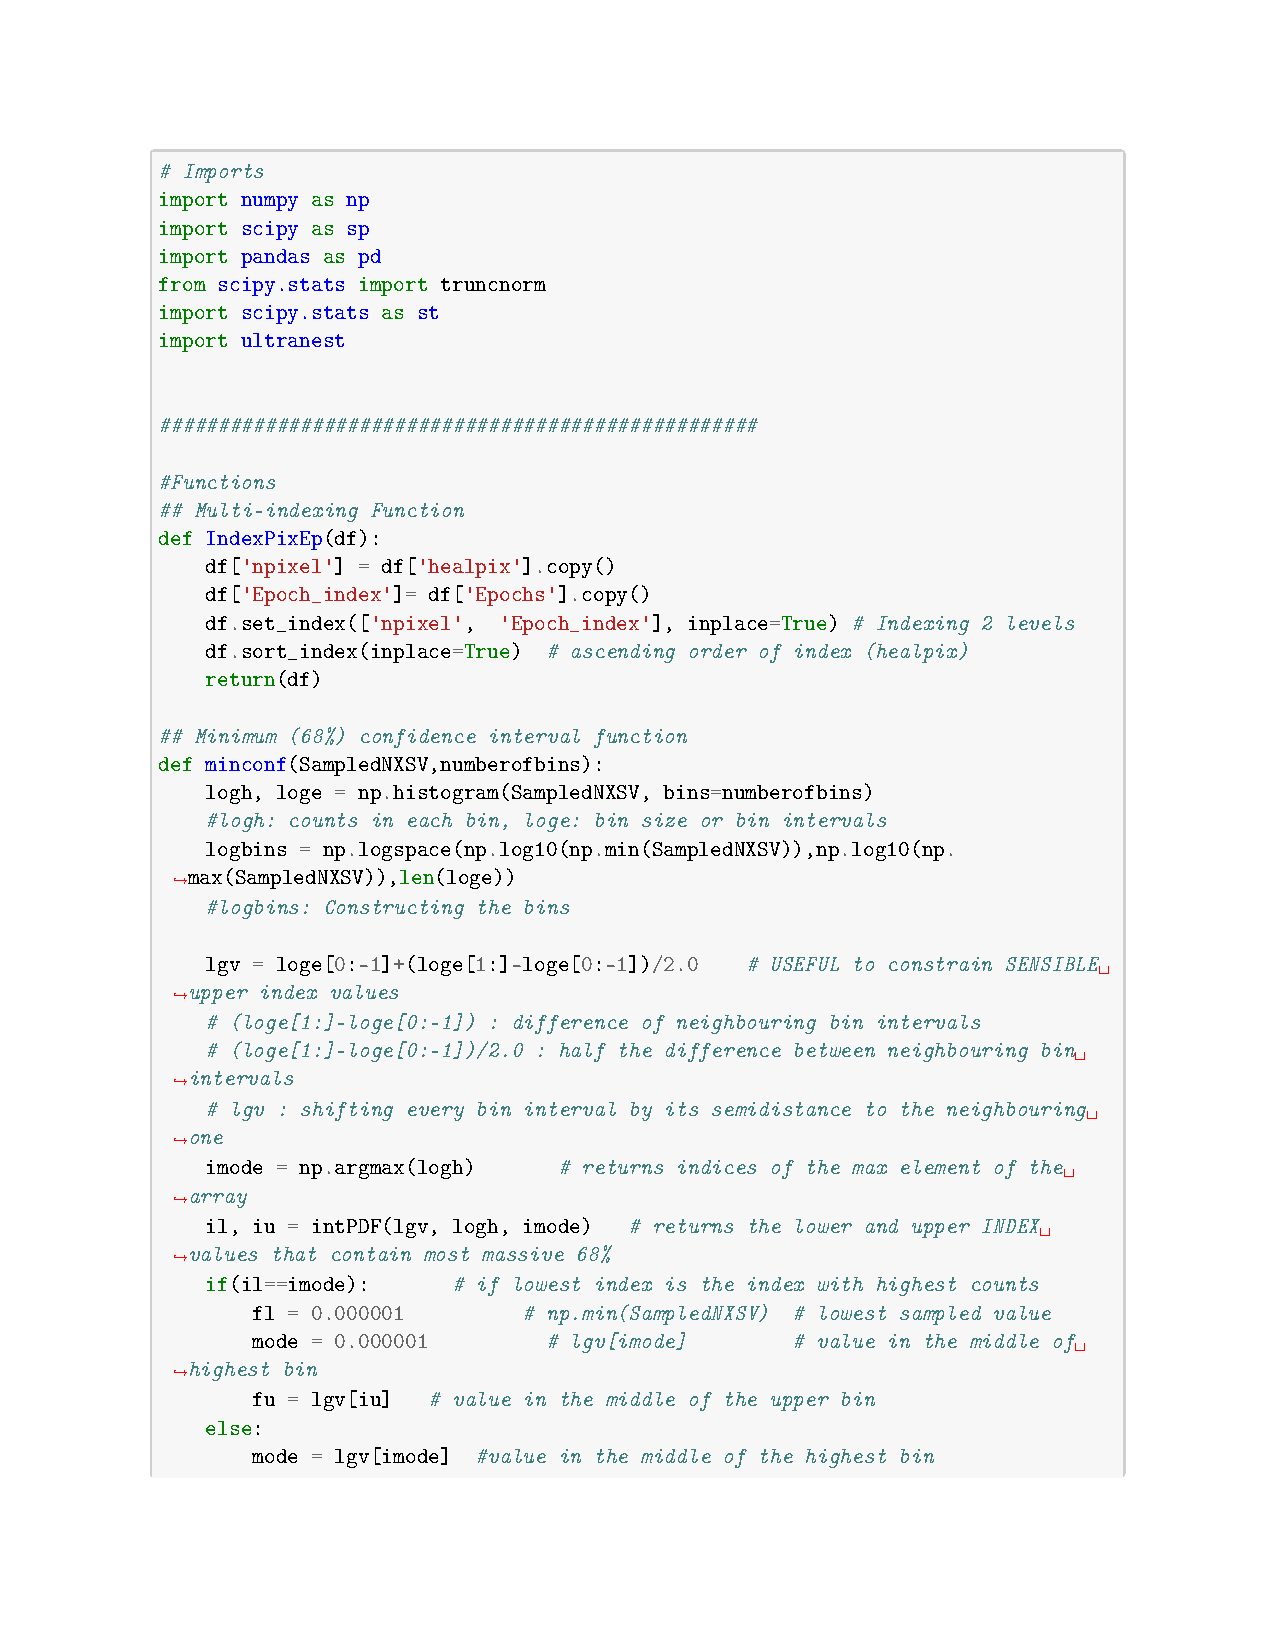
\includegraphics[width=1.0\linewidth,page=1]{Figures/Final Code Illustration-Bayesian.pdf}
\end{center}

%\begin{left}
    \includegraphics[width=1.0\linewidth,page=2]{Figures/Final Code Illustration-Bayesian.pdf}
%\end{left}

\begin{center}
    \includegraphics[width=1.0\linewidth,page=3]{Figures/Final Code Illustration-Bayesian.pdf}
\end{center}

\begin{center}
    \includegraphics[width=1.0\linewidth,page=4]{Figures/Final Code Illustration-Bayesian.pdf}
\end{center}

\begin{center}
    \includegraphics[width=1.0\linewidth,page=5]{Figures/Final Code Illustration-Bayesian.pdf}
\end{center}

\begin{center}
    \includegraphics[width=1.0\linewidth,page=6]{Figures/Final Code Illustration-Bayesian.pdf}
\end{center}
%\section{Υπολογισμός της \textlatin{NXSV} από φωτομετρικά δεδομένα}
%\section{Υπολογισμός της λαμπρότητας}
%\section{Εφαρμογή του αλγορίθμου \textlatin{Bayes}}
%\usepackage{pdfpages}
%\includepdf[pages=-]{Final Code Illustration-Bayesian.pdf}
 

	 %Εδώ μπαίνουν τα παραρτήματα
	
	\addtocontents{toc}{\vspace{2em}}  % Add a gap in the Contents, for aesthetics
	\vfil\vfil\null
		
		
		
				%% ----------------------------------------------------------------
	%\addcontentsline{toc}{\vspace{1em}}{\emph{Βιβλιογραφία}}
	%\clearpage
	%\vfil\vfil\null
	\bili \addtocontents{toc}{\vspace{1em}}
	\label{Bibliography}   %\addtocontents{toc}{\vspace{1em}}
	\lhead{\emph{Βιβλιογραφία} }  % Change the left side page header to "Bibliography"
	\bibliographystyle{ACM-Reference-Format}
	% \bibliographystyle{unsrtnat}  % Use the "unsrtnat" BibTeX style for formatting the Bibliography
	\textlatin{
		\bibliography{Bibliography}  % The references (bibliography) information are stored in the file named "Bibliography.bib"
		
			
			
		} 
		\clearpage  % Declaration ended, now start a new page
		
		
	
	
		%% ----------------------------------------------------------------
		% Declaration Page required for the Thesis, your institution may give you a different text to place here
		\Declaration{
			
			% \addtocontents{toc}{\vspace{1em}}  % Add a gap in the Contents, for aesthetics
			
			Δηλώνω ότι αυτή η πτυχιακή εργασία με τίτλο <<Μεταβλητότητα των \textlatin{AGN} στις μαλακές ακτίνες Χ: το πεδίο \textlatin{XMM-XXL-North}>> και η δουλειά που παρουσιάζεται σε αυτή είναι δικά μου. Επιβεβαιώνω ότι:
			
			\begin{itemize} 
				\item[\tiny{$\bullet$}] Η εργασία αυτή πραγματοποιήθηκε εξ ολοκλήρου κατά τον χρόνο προπτυχιακών σπουδών μου στο Εθνικό και Καποδιστριακό Πανεπιστήμιο Αθηνών.
				
				\item[\tiny{$\bullet$}] Όπου οποιοδήποτε μέρος αυτής της πτυχιακής εργασίας έχει προηγουμένως κατατεθεί για την απόκτηση πτυχίου ή άλλου τίτλου σε αυτό ή άλλο πανεπιστήμιο, αυτό διατυπώνεται ξεκάθαρα.
				
				\item[\tiny{$\bullet$}] Όπου έχω συμβουλευτεί την δημοσιευμένη δουλειά τρίτων, αυτό αποδίδεται ορθώς.
				
				\item[\tiny{$\bullet$}] Όπου έχω παραθέσει από δουλειά τρίτων, η πηγή δίνεται πάντα. Με εξαίρεση αυτές τις παραθέσεις, αυτή η πτυχιακή εργασία είναι εξ ολοκλήρου προσωπική μου εργασία.
				
				\item[\tiny{$\bullet$}] Έχω παραθέσει όλες τις κύριες πηγές βοήθειας.
				
				\item[\tiny{$\bullet$}] Όπου αυτή η πτυχιακή εργασία είναι βασισμένη σε συνεργατική δουλειά δική μου και τρίτων, έχω καταστήσει ξεκάθαρο ποιά κομμάτια έχουν πραγματοποιηθεί από άλλους και πώς συνέβαλα εγώ.	
				
				\item[\tiny{$\bullet$}] Οι κανονισμοί για την απόκτηση πτυχίου μου είναι γνωστοί. 
				
				
				\end{itemize}
				
				Η πτυχιακή εργασία που υποβάλω πραγματοποιήθηκε με την συνεργασία και επίβλεψη του Κύριου Ερευνητή του Εθνικού Αστεροσκοπείου Αθηνών Δρ. Αντώνη Γεωργακάκη και συνεπίβλεψη της Επίκουρης Καθηγήτριας του Εθνικού και Καποδιστριακού Πανεπιστημίου Αθηνών Δρ. Καλλιόπης Δασύρα.\\
				\tab\\
				Αθήνα, 2021.
				\\
			
	}		
			
			% Υπογραφή:\\
			% \rule[1em]{25em}{0.5pt}  % This prints a line for the signature
			
			% Ημερομηνία:\\
			% \rule[1em]{25em}{0.5pt}  % This prints a line to write the date
			
			
	
\end{document}  % The End
%% ----------------------------------------------------------------